\makeatletter
\renewcommand{\PackageInfo}[2]{}% Remove package information
\renewcommand{\@font@info}[1]{}% Remove font information
% \renewcommand{\@latex@info}[1]{}% Remove LaTeX information
\makeatother

\PassOptionsToPackage{unicode}{hyperref}

\documentclass[10pt]{report}
% \usepackage[margin=1in]{geometry}
% \newcommand\hmmax{0}
% \newcommand\bmmax{0}
% % % Fonts% %
% \usepackage{luatexja}

\usepackage[T1]{fontenc}
\usepackage[complete, subscriptcorrection, slantedGreek, mtpfrak, mtpbb, mtpcal]{mtpro2}
   \usepackage{bm}% Access to bold math symbols
   \usepackage[no-math]{fontspec}
   \defaultfontfeatures{Ligatures=TeX}%,Numbers={Proportional}}
   \newfontfeature{Microtype}{protrusion=default;expansion=default;}
   \setmainfont[Microtype,Ligatures=TeX,BoldFont={*-Semibold}]{Source Serif Pro}
   \setsansfont[Microtype,Scale=MatchLowercase,Ligatures=TeX,BoldFont={*-Semibold}]{Source Sans Pro}
   \setmonofont[Scale=0.8]{Source Code Pro}
   % \usepackage{selnolig}% For suppressing certain typographic ligatures automatically
% % % % % % %
\usepackage{amsthm}         % (in part) For the defined environments
\usepackage{mathtools}      % Improves  on amsmaths/mtpro2
\usepackage{xfrac}

% \usepackage{silence}
% \WarningsOff[marginnote]% Suppress warnings related to package

\counterwithout{footnote}{chapter} % For continuous footnote numbering
\counterwithout{figure}{chapter}

% % % The bibliography % % %
\usepackage[backend=biber,
  style=authoryear-comp,
  bibstyle=authoryear,
  citestyle=authoryear-comp,
  uniquename=false,
  % allinit,
  % giveninits=true,
  backref=false,
  hyperref=true,
  url=false,
  isbn=false,
  doi=false,
  useprefix=true,
  ]{biblatex}
\DeclareFieldFormat{postnote}{#1}
\DeclareFieldFormat{multipostnote}{#1}
% \setlength\bibitemsep{1.5\itemsep}
\newcommand{\noopsort}[1]{}
\addbibresource{Ability.bib}
% % % % % % % % % % % % % % %

\usepackage[inline]{enumitem}
\setlist[enumerate]{noitemsep}
\setlist[description]{style=unboxed,leftmargin=\parindent,labelindent=\parindent,font=\normalfont\space}
\setlist[itemize]{noitemsep}

% % % Misc packages % % %
% \usepackage{setspace}
% \usepackage{refcheck} % Can be used for checking references
% \usepackage{lineno}   % For line numbers
% \usepackage{hyphenat} % For \hyp{} hyphenation command, and general hyphenation stuff
\usepackage{nonumonpart} % Disable page numbers on 'Part' title pages
% % % % % % % % % % % % %

% % % Red Math % % %
\usepackage[usenames, dvipsnames]{xcolor}
% \usepackage{everysel}
% \EverySelectfont{\color{black}}
% \everymath{\color{red}}
% \everydisplay{\color{black}}
\definecolor{fuchsia}{HTML}{FE4164}%Neon Fuchsia %{F535AA}%Neon Pink
\definecolor{details}{HTML}{FE4164}%Neon Fuchsia %{F535AA}%Neon Pink
\definecolor{expand}{HTML}{C61AFF}
\definecolor{later}{HTML}{A65978}
\definecolor{return}{HTML}{660066}
% % % % % % % % % %

\usepackage[export]{adjustbox}
\usepackage{subcaption}
\usepackage{float}

% \usepackage{pifont}
% \newcommand{\hand}{\ding{43}}

\usepackage{tabularray} % For fancy table features

\usepackage{multirow}
% \usepackage{adjustbox}

\usepackage{multicol}

\setcounter{secnumdepth}{4}
\setcounter{tocdepth}{4}

% % % % % % % % % % % % TIKZ
\usepackage{tikz}
\usetikzlibrary{bending,arrows,positioning,calc,arrows.meta,patterns,fadings}
\usetikzlibrary{trees}
\usetikzlibrary{backgrounds, positioning, fit}
\usepackage{tikz-qtree} %for simple tree syntax
% \usetikzlibrary{positioning,shapes.multipart} %for structured nodes
\usetikzlibrary{tikzmark}
% % % % % % % % % % % %

\usepackage{graphicx} % for images (png/jpeg etc.)
\usepackage{caption} % for \caption* command

% \usepackage{svg}
% \usepackage[off]{svg-extract}
% \svgsetup{clean=true}

\usepackage{extarrows}

% % % % % % % % % % % % MY COMMANDS
\newcommand{\hozlinedash}[0]{%
  \noindent\hdashrule[0.5ex][c]{\textwidth}{.1pt}{2.5pt}
  %\vspace{-10pt}
}

\def\nleadsto{\mathrel{%
    \mathchoice{\NLEADSTO}{\NLEADSTO}{\scriptsize\NLEADSTO}{\tiny\NLEADSTO}%
}}
\def\NLEADSTO{{%
    \setbox0\hbox{\leadsto}%
    \rlap{\hbox to \wd0{\hss\hspace{-10pt}\not\hss}}\box0
  }}

\usepackage{dashrule}
\newcommand{\hozline}[0]{%
  \noindent\hdashrule[0.5ex][c]{\textwidth}{.1pt}{}
}
% % % % % % % % % % % %
\usepackage{xskak} % For chess diagram
\usepackage{lplfitch} % For fitch proofs

% % % % % % % % % % % %

% % % My packages % % %
\usepackage{CustomTheoremsThesis}
% \usepackage{FuturePromisedEvents}
\usepackage{ThesisCustom}
\usepackage{Notes}
% % % % % % % % % % % %

\makeatletter
\renewcommand\paragraph{\@startsection{paragraph}{4}{\z@}%
  {-3.25ex\@plus -1ex \@minus -.2ex}%
  {1.5ex \@plus .2ex}%
  {\normalfont\normalsize\bfseries}}
\makeatother

\makeatletter
\renewcommand\subparagraph{\@startsection{subparagraph}{4}{\z@}%
  {-3.25ex\@plus -1ex \@minus -.2ex}%
  {1.5ex \@plus .2ex}%
  {\normalfont\normalsize\bfseries}}
\makeatother

\usepackage[hidelinks,breaklinks,bookmarks=false]{hyperref}

\usepackage[british]{babel}
\usepackage{hyperref}
\addto\extrasbritish{
    \def\chapterautorefname{Chapter}
    \def\sectionautorefname{Section}
    \def\subsectionautorefname{Section}
    \def\subsubsectionautorefname{Section}
}
%Following commands mean autoref writes `section' rather that `subsection', etc.
%https://tex.stackexchange.com/questions/177007/autoref-showing-subsection-and-subsubsection
\let\subsectionautorefname\sectionautorefname
\let\subsubsectionautorefname\sectionautorefname

\title{
  I have the ability to \emph{V} that \emph{p}, so \emph{p}

  \mbox{ }

  {\large
    Or:
  }

  \mbox{ }

  {
    \normalsize
    I have the ability to verify the equation, so the equation is true\\
    I have the ability to demonstrate a strategy, so a strategy exists\\
    I have the ability to prove contraposition, so contraposition is a theorem\\
    I have the ability to establish that you are testifying, so you are testifying\\

    \[\vdots\]
  }
  \mbox{ }

  {\large
    But not:
  }

  \mbox{ }

  {
    \normalsize
    I have the ability to guess that it's raining outside, so it's raining outside\\
    I have the ability to be convinced that I'm lost, so I'm lost\\
    I have the ability to deny that the radio is turned on, so the radio is turned on\\

    \[\vdots\]
  }
}
\author{Ben Sparkes}
% \date{ }

\begin{document}

\pagenumbering{roman}

\maketitle

\tableofcontents

\newpage

\pagenumbering{arabic}

\part{Introduction}


\chapter{Introduction}
\label{cha:introduction}

% \section{Ability}
% \label{sec:ability-broad-intro}

\begin{note}
  \color{red}
  Some general introduction to the topic, generating some interest for cases in which agent's reasoning with ability.
\end{note}

\begin{note}[Point about ability]
  \begin{enumerate}[label=(E\arabic*), ref=(E\arabic*), series=i_ex]
  \item\label{intro:ex:algebra} If you have the ability to reason with basic algebra and radicals, then you have the ability to verify the following equation (\autoref{fig:into:eq}) it true.
  \end{enumerate}

  \begin{figure}[H]
    \[\frac{(3 + \sqrt{3})^{2} + \sqrt{6}^{2} - (2\sqrt{3})^{2}}{2(3 + \sqrt{3})\sqrt{6}} = \frac{1}{\sqrt{2}}\]
    \caption{A mercifully intimidating equation}
    \label{fig:into:eq}
  \end{figure}

  Suppose you do have the ability to reason with basic algebra and radicals --- developed, at least for me, through the public education of my youth and maintained by some chance of memory.
  Then, the antecedent of the stated conditional is true, and so the consequent of the conditional is true:
  You have the ability to verify the given equation.
  Further, you have the ability to verify the equation only if the equation is true (of course, you also have the ability to verify \emph{whether} the equation is true, but the consequent makes a stronger claim).

  So, if it is true that you have the (general) ability to reason with basic algebra and radicals then it is true that you have the (specific) ability to verify the equation is true.
  And, if it is true that you have the (specific) ability to verify the equation is true, then the equation is true.
  Hence, if it is true that you have the (general) ability to reason with basic algebra and radicals, then the equation is true.

  Of note is that you do not need to witness your (general) ability to reason with basic algebra and radicals to conclude that the equation is true.

  Of course, you may only be \emph{confident} that you have the relevant general ability.
  The same observation applies.
  As \ref{intro:ex:algebra} informs you of an application of a general ability, your confidence that you have the general ability will bound confidence in the result of applying the general ability.

  So, reformed, you do not need to witness you ability to reason with basic algebra and radicals to be confident that the equation is true.
\end{note}

\begin{note}[Focus]
  The focal point of the above is the observation that:
  \begin{enumerate}[label=(O\arabic*), ref=(O\arabic*), series=i_ob]
  \item\label{intro:obs:claim} If an agent is in position to claim support for having some (specific) ability, then the agent is in a position to claim support for the result of witnessing that ability (prior to, or independently of, witnessing that ability).
  \end{enumerate}
  This is true, in part, because:
  \begin{enumerate}[label=(O\arabic*), ref=(O\arabic*), resume*=i_ob]
  \item\label{intro:obs:entail} It would not be possible for an individual to have the (specific) ability (of the kind mentioned in~\ref{intro:obs:claim}) if the result of the witnessing the ability were not true.\nolinebreak
    \footnote{The converse does not hold, some lack the ability to reason with basic algebra and radicals --- I'm confident I lack the ability to read sheet music, though I may have been taught at one point.}
  \end{enumerate}
  Information is valuable in part because don't need to witness ability to be confident.
  Witnessing may be desirable --- check on ability, increased confidence, etc. Or, requirement as part of a test.
  Still, it doesn't seem that you need to verify in order to use the information.

  For example, let me add that:
  \[\frac{1}{\sqrt{2}} = \frac{\sqrt{2}}{2}\]
  I think you may now be confident that:
  \[\frac{\sqrt{2}}{2} = \frac{(3 + \sqrt{3})^{2} + \sqrt{6}^{2} - (2\sqrt{3})^{2}}{2(3 + \sqrt{3})\sqrt{6}}\]
\end{note}

\begin{note}[Focus and resistance]
  Focal point is about what follows from (specific) ability, when claim support for result
  Question about how important understanding of ability is.

  May think that the observed entailment~\ref{intro:obs:entail} is sufficient.
  So long as the entailment holds, there is no need to puzzle about why the entailment holds.
  Now, something about ability that secures the entailment, but given entailment there is no need to understand what that is in order to use entailment.

  Example, that the light is turned on entails that there is some source of electricity.
  Not to important to understand why this entailment holds --- I have no interest with the physical principles involved.
  What matters to me is that a source of electricity means that I might have the opportunity to charge my phone.

  May hold that \(Kp\) and logical equivalence of \(p\) and \(q\) entails \(Kq\).
  Here, understanding of \(K\) is important.
  Similarly, if the entailment does not hold.

  Proposal, then, is to argue that so long as the entailment observed in~\ref{intro:obs:claim} holds, the details of why entailment holds do not matter.

  If I had told you, then must be true in order for me to make claim.
  All that's required is second observation, and then, no need to witness because even if you don't have the ability I would have implicitly testified that the equation is true.
  So, it doesn't really matter why entailment holds for ability.
  For, confidence in result regardless.
  May still be of some interest, but worse than lights and electric circuit.
  So long as entailment holds, ability itself doesn't seem to matter.

  Likewise, usually discover ability by witnessing.
  I did not recognise I had the ability to factor \(210\) into consecutive primes before having done so.

  Here, receiving information, and I was careful not to provide such implicit testimony that the result is true.
  If you lack the ability to reason with basic algebra and radicals, then the stated conditional is true, even if you lack the ability to verify the given equation.
  So, you may lack the ability to verify the given equation (in part) because the equation is not true.
  Therefore, it seems your confidence that the equation is true is due in part to your confidence that you are able to verify that the equation is true.
  For, if you were not confident in general ability, then lack confidence that you have specific ability, and argument for truth of equation collapses.
  Hence, now appealing to the antecedent to obtain consequent.
  Still some way to go before interest in entailment, but have established in some cases, don't just need the entailment, but also the instantiation of the antecedent by the agent.
\end{note}

\begin{note}[Difficulty]
  Well, the impersonal nature of a paper allows further resistance.
  I don't have any information about who is reading, and it is possible that you do not have the (specific) ability to reason with basic algebra and radicals.
  However, there is someone who has the ability to reason with basic algebra and radicals.
  So, in order to have made a true statement, that someone must also have the ability to verify the given equation.
  And, that someone has the ability to verify the given equation only if the equation is true.
  So, regardless of whether you have the relevant abilities, the equation must be true.

  In short, even if some interest in entailment, it is not clear that \emph{your} ability matters for the entailment.
\end{note}

\begin{note}[`\emph{De dicto}' reading]
  Call the above the `\emph{de dicto}' reading of ability.
  Perhaps a slight misnomer, but the terminology effectively conveys the core idea that reference to an individual (you!) is replaced by an existential quantifier, and it is the satisfaction of the quantifier rather than reference to any particular individual which guarantees the truth of the conditional.
  So, as long as there is some person who has the ability to reason with basic algebra and radicals, then that person has the ability to verify the equation, and so the equation is true.

  Previous that I was careful to avoid didn't require a specific reading, simply observation about entailment.
  The `\emph{de dicto}' reading is more flexible.
  Independent from communication, as you're in a position to infer that the equation is true regardless of the intermediary steps.

  To illustrate, if there is someone who is a spy, then Morsel has composed some poetry.
  And, Morsel has composed some poetry only if there are horses to be spared.
  The antecedent of the first consequent is (almost certainly) true, so it must be true that there are horses to be spared, even if the consequent and intervening steps make no sense to you.
  So long as one may only have the ability to verify some proposition if the proposition is true, then this is all we need to understand about ability.

  A question remains as to whether you also satisfy property of having the ability to reason with basic algebra and radicals, but on the `\emph{de dicto}' reading of ability, this question --- like the question about the details of ability --- is only of derivative interest.
  Likewise, question about why ability has entailment, but nothing particularly interesting about claiming support prior to reasoning, because the `\emph{de dicto}' reading doesn't rest on unwitnessed reasoning.
  For example, may be that only discover ability after successful witnessing by someone, hence, given \emph{de dicto} reading, someone has verified that equation, and so by chain of entailments, reduce information to sundry observation that someone has (already) verified the equation is true.

  Some reasoning with ability is like this.
  Plausible that it's the reasoning you performed.
  And, granting the `\emph{de dicto}' reading, confidence that someone has the ability to reason with basic algebra and radicals is likely stronger than confidence that oneself has the same ability.
  It's a relief --- not only have we avoided any difficult questions about ability, but we've also excused our ability from consideration.

  However, not all reasoning with ability may be captured by the `\emph{de dicto}' reading of ability.
  Some ability statements are directed toward individuals, irrespective of whether some other person may satisfy the property of having the ability.
\end{note}

\begin{note}
  Let me try a second time --- this time I'm addressing you, and none of the other readers.\nolinebreak
  \footnote{They probably don't exist --- though it's unlikely you do either.}
  \begin{enumerate}[label=(E\arabic*), ref=(E\arabic*), resume*=i_ex]
  \item\label{intro:ex:chess} If you are able to reason with the rules of chess, then you have the ability to demonstrate that White cannot prevent Black from occupying c4 on Black's second move given the game state (described in figure~\ref{fig:chess:board:intro}).
\end{enumerate}
\end{note}

\begin{figure}[H]
  \centering
  \mbox{ }
  \hfill
  \begin{subfigure}{.4\textwidth}
    \begin{adjustbox}{minipage=\linewidth,scale=0.7}
      \centering
      \newchessgame[
      setwhite={ka5,pa3,pb4,pc4,pe5,pf6,bg5,bh5},
      addblack={pa6,pb7,pc6,pe6,pf7,kc7,nd7,nd4},
      ]%
      \setchessboard{showmover=false}%
      \chessboard
    \end{adjustbox}
    \caption{
      Game state\newline
      \mbox{ }\newline
    }
    \label{fig:chess:board:intro}
  \end{subfigure}
  \mbox{ }
  \hfill
  \mbox{ }
  \begin{subfigure}{.4\textwidth}
    \begin{adjustbox}{minipage=\linewidth,scale=0.7}
      \centering
      \newchessgame[
      setwhite={ka5,pa3,pb4,pc4,pe5,pf6,bg5,bh5},
      addblack={pa6,pb7,pc6,pe6,pf7,kc7,nd7,nd4},
      ]%
      \setchessboard{showmover=false}%
      \chessboard[
      arrow=latex, linewidth=1pt,
      shortenstart=.8ex, shortenend=.5ex,
      pgfstyle=straightmove,
      strokeopacity=0.4, fillopacity=0.4,
      color=black, pgfstyle=border,
      markfields={c4,a3,a5,g6,c5},
      ]
    \end{adjustbox}
    \caption{Example fields White cannot prevent Black from occupying after two moves.}
    \label{fig:chess:move}
  \end{subfigure}
  \hfill
  \mbox{ }
  \caption{Black to checkmate in four moves.\protect\footnotemark}
  \label{fig:chess:intro}
\end{figure}

\begin{note}

  Have a grasp of the general rules, but perhaps there's more.
  If I'm lucky, then you're like me, and I have the opportunity to say something trivially true.

  Think of me as a sibling.
  I wouldn't flat-out lie to you, but I might (intentionally) mislead you --- especially if I thought you were in an excess of confidence.

  So, assuming you know that I have a good understanding of your ability, whether or not there is a strategy for Black is a function of your confidence in your ability to reason with the rules of chess.
  If you are high confident, then a strategy exists.
  If not confident, then no clear route to whether a strategy exists.

  Return to the reasoning above.
  Call this `\emph{de re}' understanding of ability.

  In contrast to `\emph{de dicto}', interest in how ability works.
  Because, now it's your ability to reason with rules of chess.
  And, given information your ability to demonstrate the existence of a strategy.
  And, why this should allow result granting the possibility of mistake.
\end{note}

\begin{note}[More examples, and narrowing]
  Our interest is with the `\emph{de re}' reading of ability.

%   Two examples given, general phenomena.

%   Handful more.
%   \begin{enumerate}
%   \item You have the ability to recognise that performing that action is a bad idea. (It's a bad idea.)
%   \item If you are able to program this C then speed up. (Speed up.)
%   \item You're able to make that argument only if you're able to defend this premise. (I am able to provide a defence of the premise.)
%   \end{enumerate}
%   Focus on mental activity.
%   \begin{enumerate}
%   \item You have the ability to run a 5k.
%   \item If you are able to hit the center of the dartboard, you win a prize.
%   \item You're able to change lanes only if you're able to raise your speed by 20km/h.
%   \end{enumerate}
%   These cases, either dead-end in ability, or state result of witnessing ability.
%   No clear divide.
%   \begin{enumerate}
%   \item If you are able to answer all of the questions, then pass the test.
%   \end{enumerate}
%   In cases of interest, something independent of ability must be true in order for agent to have ability.
  Returning to~\ref{intro:obs:claim} and~\ref{intro:obs:entail}.

  \gsi{}, and your (specific) ability does the work.
  Observation made above, confidence, and wouldn't have ability if result wasn't (independently) true --- does truth of equation or existence of strategy holds regardless of whether you witness ability that you're confident you have.
  Something more to be said about this observation as it is \emph{your} ability that is granting the result.

  Ability applies to a verb.
  Two verbs used `verify' and `demonstrate' are both factive.
  So, here's an account of why result holds.
  Verify or demonstrate only what is (already) true.

  However, prior observation that ability applies to an action that's of real interest.
  Verb.
  On interpretation of interest, if agent is in position to claim support for (specific) ability, then agent is in a position to witness the ability.
  For example, if you able to reason with basic algebra and radicals, then do not need to learn anything further about algebra or radicals to verify the stated equation.
  Likewise, if you able to reason with the rules of chess, then you do not lack any information required to show that a strategy exists.

  Given our interest is with reasoning, express this by stating that the agent is in a position to claim support for a collection of premises and steps of reasoning whose arrangement would be sufficient to claim support for the result.

  Of course, may take some time, explore a few dead-ends, or you may run out of patience --- no guarantee that you will witness ability.
  Still, there is a path from resources at your disposal to the desired result.

  Third observation
  \begin{enumerate}[label=(O\arabic*), ref=(O\arabic*), resume*=i_ob]
  \item\label{intro:obs:resources} Interpretation of interest, sufficient resources are available to the agent for (specific) ability.
  \end{enumerate}
  The agent is in position to witness their ability.
  Not all ability carries this implication, and it may be difficult to determine whether any isolated does.
  Still, relation between general and specific ability helps clarify.

  XXX

  So, on the one hand, confidence that you have the (specific) ability, and on the other hand confidence that you are in a position to witness the (specific) ability.
  And, witnessing, then support claimed on the basis of available resources.

  Two different ways of understanding `\emph{de re}'.
  Term these \AR{} and \WR{}, respectively.

  Distinction is motivated by verb.
  Ability, so there's something agent may do.
  And, given examples, claim support for result prior to doing whatever it is that the agent is able to do.

  And, if \WR{}/result of verb, then support claimed isn't from ability, but the premises and steps.
  If you were to verify or demonstrate, would not appeal to ability.
  Role of ability in \WR{} is to inform that resources are available.

  \AR{}, by contrast, only required premise.
  Ability nominalises verb, property like any other, and this combined with above observations does the work.

  An analogy may be helpful.
  Think of the distinction between \AR{} and \WR{} as akin to the distinction between the mention and use of a term.

    For example, I may mention the term `questionable', and note that `questionable' contains an instance of each vowel.
  Or, I may use the term `questionable' by stating that it is questionable whether an agent may always appeal to having some (specific) ability when claiming support for the result of witnessing the ability.
  However, when I report that the readers of this thesis found questionable, goes to a use.
  There was some event, in which term was mentioned and used to communicate something.
  To understand implications, need to consider use.

  Question is whether the latter observation holds for ability.
  Does the result follow because claiming support having the ability is sufficient to claim support for conclusion --- in line with \AR{}.
  Or, does the result follow because you are in a position to claim support by witnessing ability and hence claim support from premises and steps.

  So, two interpretations of `\emph{de re}' reading of ability.
  \AR{}, result follows from the agent having a property.
  \WR{}, result follows from event that agent is in a position to witness.
\end{note}

\begin{note}
  What separates the \AR{} and \WR{} interpretations of `\emph{de re}' reading of ability?
  In short, constraints on when an agent may claim support for a proposition.

  Unfortunately, details beyond the scope of an introduction matter.
  

  \WR{} understanding of ability conflicts with simple understanding of when an agent may claim support.

  \begin{enumerate}[label=(O\arabic*), ref=(O\arabic*), resume*=i_ob]
  \item\label{intro:obs:uRa} An agent may claim support for the result of reasoning only if the agent has reasoned from premises to conclusion.
  \end{enumerate}
  If~\ref{intro:obs:uRa}, then \WR{} is ruled out, as the~\ref{intro:obs:uRa} requires the agent to witness the reasoning that they are (confident that) they are able to perform.

  Hence, \AR{}, that the agent has the ability is a premise in any reasoning.
\end{note}

\begin{note}[Interest in~\ref{intro:obs:uRa}]
  Notable in many accounts of the basing relation.
  Also, rationality and so on.
  Requires a step that I will not argue for --- that if successful in claiming support by structure, then inherit support by structure.
  Consider this plausible.
  Talk of claiming so may remain neutral on what support is.
  Doesn't matter whether internalist or externalist from premises and steps, etc.\
  \AR{} and \WR{} are structural.

  Primary argument is conflict.
  \ref{intro:obs:uRa} requires \AR{}, but \AR{} is incompatible with minimal understanding of claiming support.
  Roughly, that agent does not require truth of proposition or existence of support in order to claim support for that proposition.\nolinebreak
  \footnote{
    Note, this does not entail that support is always available.
    If don't own a dog, then there may be no information available for neighbour to claim support that you own a dog.
    Rather, neighbour is not in a position to claim support if recognised by neighbour that X only supports if you already have a dog.
  }
  Internalist?
  No.
  Don't need it to be true that visual perception is reliable to be in a position to claim that something \dots.
  Externalism in part because this is support does not follow from claiming support.

  Conflict isn't so straightforward.

  \begin{enumerate}[label=(O\arabic*), ref=(O\arabic*), resume*=i_ob]
  \item\label{intro:obs:nI} An agent is never in a position to claim support for truth of a proposition \(\psi\) given claimed support for some proposition \(\phi\) by observing that \(\psi\) must be true if \(\psi\) is true when:
    \begin{enumerate}[label=(\alph*), ref=(O\arabic{enumi}\alph*)]
    \item\label{intro:obs:nI:pFalse} Possible \(\psi\) is false
    \item\label{intro:obs:nI:inclusion} Support claimed for \(\phi\) `includes' support claimed for \(\psi\)
    \end{enumerate}
  \end{enumerate}
  `Includes' is a detail.
  Roughly, basic algebra and radicals includes support for verification.
  Likewise, rules of chess includes particular strategy.

  Intuitively, not in a position to claim support for \(\psi\) for else support for \(\phi\) would be problematic.\nolinebreak
  \footnote{
    Details are particularly important here.

    Note, for example, that it seems support claimed for an agent knowing \emph{p} would be problematic were \emph{p} false, but equally my belief that you know \emph{p} seems sufficient to form a belief that \emph{p} --- though \emph{p} may be false given that I only believe that you know \emph{p}.

    The `inclusion' requirement \ref{intro:obs:nI:inclusion} means that the constraint does not immediately apply.
    If I am a layperson, then being in a position to claim support that an expert has testified that \emph{p} does not clearly allow me to claim support for \emph{p} from the resources used to claim that the expert has testified.
  }

  The constraint~\ref{intro:obs:nI} builds on the intuitive idea that an agent is never in a position to claim support for some proposition \(\psi\) on the basis that there would be a problem in having claimed support for some other proposition \(\phi\) were \(\psi\) not the case.

  Restructuring previous:

  \begin{enumerate}[label=(E\arabic*), ref=(E\arabic*), resume*=i_ex]
  \item\label{ex:nI:int:valid} So long as there is no problem in you claiming support for the ability to reason with basic algebra and radicals, then the equation is valid.
  \item\label{ex:nI:int:chess} So long as there is no problem in you claiming support for the ability to reason with the rules of chess, then you a strategy exists.
  \end{enumerate}

  It seems that you may not claim that the equation is valid from~\ref{ex:nI:int:valid} and confidence that you are able to reason with basic algebra and radicals.
  Likewise, it seems you may not claim that a strategy exists because you are confident that you are able to reason with the rules of chess and~\ref{ex:nI:int:chess} requires that a strategy exists unless there is some problem in your claim to support.

  \ref{intro:obs:nI} follows because if agent goes by truth, then they already need to hold that they have support for \(\psi\) prior to moving to the truth of \(\psi\).
  Hence, observing truth is similar to claiming no problem with claimed support for \(\phi\).

  Still, both~\ref{ex:nI:int:valid} and~\ref{ex:nI:int:chess} seem problematic in a way that~\ref{intro:ex:algebra} and~\ref{intro:ex:chess} do not.
  Indeed, both~\ref{intro:ex:algebra} and~\ref{intro:ex:chess} provide information about inclusion.
  Yet, similar feature.
  If \WR{}, then no need to make any claim about whether or not support is problematic, support for result because resources.

  The difficult part is showing that \AR{} violates~\ref{intro:obs:nI}.
\end{note}

\begin{note}
  Goal is to argue that~\ref{intro:obs:nI} follows from a minimal understanding of claiming support.
  If so, ~\ref{intro:obs:uRa} and the minimal understanding of claiming support are in tension.
  For, given that~\ref{intro:obs:uRa} requires \AR{} while \AR{} violates~\ref{intro:obs:nI}.
  Upshot, motivate \WR{} understanding of ability as exception to~\ref{intro:obs:uRa}.

  Alternative remains possible.
  However, with \WR{} well motivated exception to~\ref{intro:obs:uRa}.
  With \AR{}, struggle to find plausible alternative.

  Put it this way:
  \WR{},~\ref{intro:obs:uRa} may be mostly correct.
  If \AR{}, then mostly incorrect about support.

  This is the negative argument.
  \WR{} because alternative is worse.
  Main focus.

  Supplementary is positive argument.
  \WR{} provides novel insights in a number of areas.
\end{note}


\begin{note}
  In \WR{} understanding, agent appeals to premises and steps of reasoning that they would access were they to witness ability.
  Of course, prior to witnessing, agent does not have information about what these are.

  Surprising, because exceptions to~\ref{intro:obs:uRa}.

  Even if no particular interest in details of reasoning with ability, broad consequences given~\ref{intro:obs:uRa}.
\end{note}

\begin{note}[GSI]
  Of course, not all cases generate such interest.
  Consider consequent alone:
  \emph{You have the ability to demonstrate that a strategy exists for Black}.
  In order to claim, strategy must exist.

  Term the type of conditionals `\gsi{}'.
  General, so support for ability, and specific, use of ability to obtain result.
  Interest because confidence from general leads to confidence for specific, and then result, with no other route to result.

  \gsi{} highlight cases in which ability really does something, and if argument is successful then plausible applies to `direct' information about ability, such as in the isolated statement of the consequents or examples given.
\end{note}

\begin{note}[Ideal and non-ideal]
  Ideal agents have no need for ability.
  Non-ideal agents do.
\end{note}

\begin{note}
  Main contributions are:
  Ability, specifically the ability to reason.
  Limitation on claiming support.
  Argument against~\ref{intro:obs:uRa}.
\end{note}

\begin{note}[Nothing comes for free]
  Rests on an understanding of claimed support.
  About claiming support, and limitation of support.
  Basic, clarity, neutral.

  True to the preface paradox, I do not think I have smuggled in strong claim, but I'm not confident to hold that the notion developed is fully general.

  Here, either uninteresting, or room for understanding of ability that does not require \WR{}.
\end{note}

%%% Local Variables:
%%% mode: latex
%%% TeX-master: "master"
%%% End:


\part{Overview}

%%% Local Variables:
%%% TeX-master: "master"
%%% End:

\chapter{Overview}
\label{cha:overview}

\section{Outline}
\label{sec:outline}

\begin{note}
  In this chapter we provide a high level overview of the main arguments made in this thesis.
  A significant part of the high level overview of arguments is an overview of the premises and assumptions that those arguments rest on.

  By given high level overview, clarify on how premises, assumptions, and conclusions relate.
  In the main body of the thesis, afford to elaborate.
  And, allow choice of where to seek elaboration.
\end{note}

\begin{itemize}
\item Start with claiming support, used throughout, so important.
\item Introduce and motivate plausible constraint on support, to be argued against/exception for.
\item Outline exception.
\item High level overview of argument for exception.
\item Major and minor.
\item Largely fairly high level sketch of major argument.
\item Type of ability information.
\item Understanding \emph{de re} ability reading.
\item \AR{} and \WR{}.
\item For the moment, brief, much more detail in relevant chapter.
\item Relation between \AR{} and \uRa{}.
\item Constraint on reading of ability.
\item Requires argument for \WR{}.
\item Introduce \nI{}.
\item Sketch argument for \nI{}.
\item Link \nI{} and \AR{}.
\item Completes overview of major argument.
\end{itemize}

\section{Ability and access to claimed support}
\label{sec:abil-access-supp}

\begin{note}
  Following introduction, interest is with ability.
  In particular, observation that \gsi{} information, and confidence in general ability seems to allow agent to claim support for result.

  Question on what basis the agent claims support.

  Slightly more general statement.
  \begin{quote}
    When and why an agent may claim support for the result of reasoning that the agent has not witnessed.
  \end{quote}
  Ability claims of interest provide some answer to `when'.
  For, ability provides information about what the result is, and also that the agent has the opportunity to perform the reasoning.\nolinebreak
  \footnote{No claim to necessity}

  Suggested in introduction, answer to `why' is more complex.
  % \begin{quote}
  %   Our interest is in when an agent may claim support for some conclusion of some instance of reasoning on the basis of the support the agent may claim for the premises of the instances of reasoning.
  % \end{quote}
\end{note}

\begin{note}[Introducing support]
  Initial clarification is with respect to claiming support.
  Emphasis on `\emph{claim}'.

  The thesis is not about when and why an agent \emph{has} support for the result of reasoning that the agent has not witnessed.

  Two reasons for this.
  First, neutral for main thread of argument on what support amounts to.
  Interest is with structure of claim, and background assumption that if success in claiming then structure of support follows structure of claim.

  Second, whether or not an agent has support often seems secondary.
  To illustrate:
  It may be that any claimed support for a proposition is support for that proposition, but perhaps not.
  Suppose `flan' is written on the side of a container.
  I may claim support that the container contains flan.
  And, it may be that the writing on the side of the container is support for the box containing flan.
  However, the straps ensuring the container remains closed is unfortunately placed, and if moved would reveal the side of the container reads `flannels'.
  The unfortunate placing of the straps does not seem to prevent \emph{claiming} support, but I'm not sure whether it is right to say that the writing on the side of the box (straps in place) \emph{does} the box containing flan.
  So, in what follows I will speak in terms of claiming support, and leave open whether what is claimed reflects on whether an agent has support.\nolinebreak
  \footnote{
    In particular, claiming allows focus on internal constrains, while remaining silent on whether having support is (in part) determined by external factors.
  }
  \(^{,}\)\nolinebreak
  \footnote{
    Distinction between propositional and doxastic support.
    Propositional, support agent has whether or not made a claim.
    Doxastic is successful claim and propositional support.
    So, both require that the agent has support.
    Claimed support is the agentive component of doxastic support.
    Not interested in whether the agent also has propositional support, though more or less assume.
  }
  \(^{,}\)\nolinebreak
  \footnote{
    {
      \color{red}
      English is somewhat difficult.
      It is somewhat unfortunate that `an agent has claimed support for \(\phi\)' may be read `there is support which the agent has claimed for \(\phi\)'.
      Still, this seems to follow more easily from `support claimed'.
      So, `claimed support' emphasises the claim, while `support claimed' emphasises support.
    }
  }
\end{note}

\subsection{Background for claiming support and reasoning}
\label{sec:claimed-support}

\begin{note}[Understanding of claiming support]
  Understanding of claiming support.

  Begin with a sufficient condition.
  In short, most instances of reasoning.
  Claiming support is common.

  Then, two types of defeaters.
  Mistaken and misled.
  Use to form a necessary condition.
  If claimed support, then agent deems that claimed support is not defeated.
  `Deem' is a placeholder.
  Strong or weak.
  Single constraint is that when claiming support, potential defeaters that aren't ruled out.\nolinebreak
  \footnote{
    At least two ways of viewing this.
    First, claiming support is restricted.
    Second, \emph{claiming} support only applies when there are potential defeaters, and some other relation to support when possible defeaters get ruled out.

    These are different, but I don't think the difference matter for resource bound agents of interest.
    Lack of resources is that always potential defeater, even if every possible defeater may be ruled out.
    }
  Finally, property, that claimed support does not depend on whether proposition the agent has claimed support for is true, or whether the claimed support \emph{does} support (if these are separated).
  Property will be important.
\end{note}

\begin{note}[Sufficient condition]
  We start with a sufficient condition for claiming support:
  \begin{proposition}[\bP{-} --- \bP{}]\label{prem:bP}
    If an agent may claim support for premises and steps of reasoning, accesses those premises and traces claim to support through those steps of reasoning, then agent may claim support for conclusion on basis of the claimed support for the steps and premises of reasoning.
    (Given that the agent deems that the claims to support for premises and steps used are undefeated when drawing conclusion.)
  \end{proposition}

  The purpose of taking~\bP{} as basic is to fix a basic understanding of when an agent may claim support.
  In short, an agent may claim support when reasoning goes well.
  And, reasoning goes well when there are premises and steps of reasoning available to the agent, and the agent draws on these to claim support for the conclusion.
  The parenthetical remark is a simple safeguard, the agent does not lose a claim to support for the premises or steps in the process of reasoning.\nolinebreak
  \footnote{
    May think that this is the wrong safeguard.
    Consider the liar paradox:
    `This sentence is false.'
    \bP{} prevents agent from claiming support that the sentence is true or false.
    However, may think that agent is in a position to claim support that the sentence is both true and false.
    Indeed, standard reasoning associated with the liar suggests that the sentence is both true and false.
    Still, it's not obvious from demonstrating that the sentence is both true and false that one may claim support for the sentence being true and the sentence being false.
    That is, one may confine the paradox to the truth value of the sentence, rather than (associated) surplus of support.
  }
  We consider defeaters below.
  First, an illustration.


  Suppose an agent measures that the box in front of them has the dimensions of \(19\text{cm}\) by \(7\text{cm}\).
  The agent understands how to calculate the area of a box, and by performing some reasoning comes to hold that the area of the box is \(133\text{cm}^{2}\).
  The support the agent has for holding that the area of the box is \(133\text{cm}^{2}\) is obtained (at least in part) on the measurement of box, understanding how to calculate the area of box, and some grasp of arithmetic.

  Whether some (or all) of the required arithmetic is to be included as a premise or a step of reasoning may be set aside.
  Similarly, set aside whether further arguments, or whether some premises and steps are taken as basic.
  For example, perhaps some the agent requires some further claim to support for using the ruler to measure the box such as comparison to a standard, or perhaps the agent's claim to support terminates by noting that their use of the ruler is a reliable process.
\end{note}

\begin{note}[Value proposition]
  Reasoning and claims to support focus.
  Briefly introduce a pair of propositions to clarify claim to support and reasoning.

  \begin{proposition}[Claimed support is for the value of a proposition]\label{prop:csifvoap}
    When an agent claims support for some proposition, the agent claims that the proposition has some value.
    Where:
    \begin{itemize}
    \item A proposition is some state of affairs. And,
    \item A value is an assessment of a state of affairs.
    \end{itemize}
  \end{proposition}
  The role of \autoref{prop:csifvoap} is primarily to fix terminology.
  To illustrate, when stating the conclusion of the reasoning sketched above we used the proposition that \emph{the area of the box is \(133\text{cm}^{2}\)}.
  The proposition refers to the state of affairs in which the area of the box is \(133\text{cm}^{2}\), and speaking a little more precisely, the agent claimed that the proposition has the value `true' --- though it may be the value turns out to be `false'.
  Or, perhaps if the agent was a little unsure about the accuracy of the ruler, that the proposition has the value `likely', `probable', or some quantitative credence.
  And, some other instance of reasoning may have concluded that the proposition has the value `desirable' --- e.g.\ if the agent was searching for a box of some approximate size.\nolinebreak
  \footnote{
    Nothing in particular hangs on the distinction between different values.
    If you prefer, you may expand the proposition (state of affairs) to include additional factors, and consider only the values `true' and `false'.
    For example, the proposition that \emph{I desire the bath to be warm} is false, as opposed to the proposition that \emph{the bath is warm} is valued undesirable by me.
  }

  Core idea is that claim of support is that things are a certain way.
  Proposition, what the thing is.
  Value, the way it is.
  In most cases the value will be clear (i.e. that the proposition is true, though sometimes that the proposition is desirable), and so we will talk of claiming support for the proposition.
  A handful of additional examples will be provided when illustrating the next proposition.
\end{note}

\begin{note}[Reasoning proposition]
  \begin{proposition}[Reasoning as establishing value]\label{prop:RisTV}
    Reasoning, tracing value through propositions/establishing that proposition has value.
  \end{proposition}

  \begin{itemize}
  \item Testimony, so claim support that \emph{p} is true.
  \item Unreliable, so claim support that \emph{p} improbable.
  \item Religious text, so claim support that \emph{p} ought to be the case.
  \item Producer, so claim support that album is desirable.
  \end{itemize}

  In a deductive case, if the premises are true, then the conclusion is true.
  Means-end reasoning for desire.
  The value is important.
  If it is true that it past 6pm, then it is true the shop is closed.
  Provides value of shop being closed.

  However, if agent desires that it is past 6pm, then it doesn't follow that the agent desires that the shop is closed.
  Question an agent as to why they think their desires conform to truth --- is-ought problem.

  Means-end reasoning.
  It is true that there is cheese at the centre of the maze.
  And, it is desirable that I obtain the cheese at the centre of the maze.
  Further, it is true that I may only obtain the cheese at the centre of the maze by solving the maze.
  Therefore, it is desirable that I solve the maze.
\end{note}

\begin{note}[Moving to value]
  \color{red}
  Important to note is that way in which agent claims support is important.

  Preface paradox.
  Here, move to value, but these are isolated.
  Don't get to combine these together, no allowed to hold that these are simultaneously true.
  Or, simultaneously assign value to the individual propositions.

  So, move isn't free, so to speak.
\end{note}

\begin{note}
  \begin{proposition}[Defeaters for claimed support]
    There are at least two ways in which a claim to support may be defeated.
    \begin{itemize}
    \item Claimed support may (discovered to be) be \emph{misled} by suggesting that a proposition has some value that it does not (in fact) have. And,
    \item Claimed support may (discovered to be) be \emph{mistaken} by appealing to factors that do not indicate the value of the proposition.
    \end{itemize}
  \end{proposition}
  Misleading support may indicate value, and value may have value indicated by mistaken support.
  Both are defeaters in the sense that, were the agent to learn that the claim to support was misleading or mistaken, then the agent would not hold that the proposition has the value indicated by the (problematic) claim to support or the basis of that (problematic) claim to support.

  Common to distinguish between countervailing and undercutting defeaters.
  Countervailing, support for some other proposition.
  Undercutting, force of claimed support is mitigated.

  Both misled and mistaken are instances of being undercut.
  For, if mistaken or misled then the support is no good.

  Neither are clearly cases of countervailing.
  For, no relation to other support is required.
  However, presence of countervailing implies misled.
  Countervailing does not imply mistaken, though may in some cases demonstrate so.

  Below suggest that when claiming support the agent excepts that claimed support is not misleading or mistaken.
  Hence, given that countervailing implies misled, implicitly take claimed support for a proposition to indicate absence.
  (This is another purpose from separation from support.)

  ???
\end{note}

\begin{note}[M\&M Illustration]
  To illustrate:

  Suppose I glance at the clock on the wall.
  The clock reads 11:45a, so I claim support that it is 11:45a.
  However, it may be the case that the clock is incorrectly set, and the time is 11:15a, or 12:15p, etc.\
  By claiming support from the time expressed by the clock, I would have been \emph{misled} about what the time actually is.
  For, it is not true that the time is 11:45a.
  Though, in all other respects, there may be no fault with claiming that the time is as expressed by the clock and so the claim to support is not mistaken.

  By contrast, suppose I glace at the clock on the wall.
  The clock reads 11:45a, so I claim support that it is 11:45a.
  By claiming support from the time expressed by the clock, I would have been \emph{mistaken} about what the time actually is.
  For, the time expressed by a broken clock is not a good indicator of what the time actually is.
  Though, despite the clock being broken, it is 11:45a and so the claim to support is not misleading.

  And, claimed support for the time from a broken clock expressing the wrong time would be both misled \emph{and} mistaken.\nolinebreak
  \footnote{
    A second illustration:
    Consider a smoke detector, designed to sound an alarm if and only if sufficient levels of smoke are detected.
    Hence, if the alarm sounds, one may claim support there being smoke in the room where the alarm is installed.
    One may be misled; the alarm may have malfunctioned, so no fire.
    Or, one may be mistaken; the same type of alarm may be installed in a different room, wouldn't be a useful indicator.
  }
\end{note}

\begin{note}[Subjectively sound]
  Of course, clocks are typically glanced at, and a glance at a clock is often insufficient to determine whether the clock is incorrectly set or broken.
  Hence, the \emph{possibility} that a clock is incorrectly set or broken --- or more broadly the possibility that claimed support is misleading or mistaken --- does not prevent an agent from claiming support.
  So, ensuring that to-be-claimed support would be neither mistaken or misleading is not a necessary condition for claiming support.
  Rather, we endorse the following condition with respect to these types of defeaters:

  \begin{proposition}[Adequacy of claimed support]\label{prop:CSNMORM}
    If agent claims support for some proposition, then
    % from the perspective of the agent,
    the agent deems that the claimed support
    % adequate whether or not the claimed support may (in fact) be
    is not misleading nor mistaken --- the agent has some expectation that possible defeaters (of the two types of noted) do not obtain.\nolinebreak
    \footnote{
      Stronger than distinct claim that the agent does not deem that the claimed support is misleading or mistaken.
      Stronger requires, presence of some deeming.
      Later does not.
    }
  \end{proposition}
  If some expectation that they do, then this seems enough to deny support.
  If no attention to defeaters, questionable whether any claimed support.

  If the claimed support is not misleading, then the proposition has the value the claimed support indicates the proposition has.
  And, if the claimed support is not mistaken, then the claimed support indicates the value.
\end{note}

\begin{note}[Agents are fallible]
  The missing piece of \autoref{prop:CSNMORM} is an account of what `deem' amounts to.
  The following proposition (\ref{prop:fallibility}) states an assumption, which allows a (general) functional characterisation of `deem'.

  \begin{proposition}[Agents are fallible]\label{prop:fallibility}
    When claiming support for a proposition and agent is never in a position to rule out the (epistemic) possibility that the claimed support is not misled or mistaken.
  \end{proposition}

  I take it to be intuitive that agents are fallible in many cases of claiming support.
  It is not too difficult to think of ways in which claimed support may be misleading or mistaken.
  As noted above, claiming support for what the time is from glancing at a clock seems sufficient, but clocks may be incorrectly set (misled) or broken (mistake).
  Similarly, a sample of \(1,000\) rolls may mislead me into thinking that a die is unbiased, or an overloaded operator may lead to a mistake in claiming support for the proposition that \(x = 4\) is an expression of equality rather than variable assignment.

  \autoref{prop:fallibility} states that an agent is never in a position to rule out the possibility that the claimed support is not misled or mistaken.
  This does not entail that there are defeaters, nor that there are any possible defeaters --- only that defeaters are an epistemic possibility.

  Still, in some cases, this may seem absurd.
  Suppose in front of me are two apples and two pears.
  So, four pieces of fruit.

  However, those appears and pears may not be real pieces of fruit, they may be replicas.
  So beings the process of attempting to quarantine fallibility from infallibility.

  There are two pairs of objects in front of me, and the objects appear to be fruit.
  So, there are four objects in front of me, which appear to be fruit.

  There are two pairs of objects hence there are four objects.

  But I may be hallucinating.

  There appear to be two pairs of objects in front of me, which appear to be fruit.
  So, there appear to be four objects in front of me, which appear to be fruit.

  Whenever there are two pairs of objects, there are four objects.

  Even so, I'm not in a position to rule out the possibility that arithmetic is inconsistent.

  Perhaps identity is a stronger candidate: Any object is identical with itself --- but I doubt one needs to claim support for reflexivity of equality.
  Similarly, it doesn't seem to be the case that I need to claim support for the proposition that my name is ミスタ --- no matter what my birth certificate says, I get to decide what my name is.

  Rather than fix a specific account of the `possibility' modal used, here are a handful compatible interpretations:

  \begin{enumerate}[label=\Alph*., ref=(\Alph*)]
  \item\label{CS:I:Never} \emph{In principle} it is not possible for any agent to rule out the possibility that claimed support is not misleading or mistaken.
  \item\label{CS:I:Resources} It is not possible for a \emph{resource bound agent} to rule out the possibility that claimed support is not misleading or mistaken.
  \item\label{CS:I:Class} There is a restricted class of propositions for which and agent is required to claim support, and it is not possible for any agent to rule out the possibility that claimed support for a proposition belonging the class is not misleading or mistaken.
  \end{enumerate}

  To illustrate, consider the proposition that there is an external world:
  \ref{CS:I:Never} denies that there could be, e.g.\ proof of an external world.
  \ref{CS:I:Resources} denies that agents of interest could not demonstrate such a proof even if it were to exist.
  \ref{CS:I:Class} allows an agent may not be required to claim support for the existence of an external world.

  I expect the intended application of claimed support will be compatible with each interpretation, and specifically with respect to \ref{CS:I:Class}, that the propositions will belong to the highlighted class.\nolinebreak
  \footnote{
    I favour the combination of \ref{CS:I:Resources} and \ref{CS:I:Class}, and to leave open whether an idealised agent may rule out the possibility of being misled or mistaken with respect to some propositions when claiming support.
  }\(^{,}\)\nolinebreak
  \footnote{
    In particular, true of ability.
  }
\end{note}

\begin{note}
  Given some interpretation of the possibility modal, the functional role of `deem' is to provide resistance to possible defeaters that an agent is not in a position to rule out.
  How resistant the agent's claimed support needs to be is up to you.

  Provide a test below to help with intuition.
  Before doing so, final proposition, which follows as a corollary from previous.
\end{note}

\begin{note}[\eiS{}]
  Subjectively sound, claimed support indicates value.

  Final proposition.
  Definition.

  \begin{definition}[Dependence and independence]
    An agent's claimed support for \(\phi\) \emph{depends} on some value of \(\psi\) just in case the agent would not claim support for \(\phi\) given any other value of \(\psi\).

    An agent's claimed support for \(\phi\) is \emph{independent} of \(\psi\) just in case the agent's claimed support does not depend on the value of \(\psi\).
  \end{definition}

  Claiming support is independent of value.

  \begin{proposition}[\eiS{-} --- \eiS{}]\label{prop:supp:independence}
    If agent claims support for some proposition, \(\phi\), then the claimed support is taken to indicate the value of \(\phi\) independently of the value of \(\phi\) or whether the claimed support is `genuine' support.
    Equivalently, the claimed support is taken to indicate the value of \(\phi\) does not require that the claimed support is not misled or mistaken.\nolinebreak
    \footnote{
      Possibly goes against externalism, but I don't think this is right.
      External circumstances may impact the support the agent has.
      However, as these are external, it seems this condition plausibly holds for \emph{claiming} support.
      This is how you get puzzles for externalism.
      In both cases, it's fine for the agent to claim support, but the external circumstances impact whether the agent \emph{has} support.
      The internalist/externalist divide would seem to affect the conditions on claiming.

      Way to expand on this is reconstructing bootstrapping examples with and without \eiS{}.
      If the agent would only get basic support if reliable, then it's not clear that bootstrapping is a problem.
    }\(^{,}\)\nolinebreak
    \footnote{
      One way independence.
      Not clear that value is independent of support.
      So long as sufficiently strong support, not possible for proposition to have value other than claimed support.
    }
  \end{proposition}
  \eiS{} follows from Propositions~\ref{prop:CSNMORM} and~\ref{prop:fallibility}.

  From Proposition~\ref{prop:CSNMORM}, deemed that claimed support is neither mistaken nor misled.
  From Proposition~\ref{prop:fallibility}, always possibility.

  Suppose depends on value of \(\phi\).
  Still, from Proposition~\ref{prop:fallibility}, (epistemic) possibility that value of \(\phi\) differs.
  If differs, then claim to support is misleading.
  By Proposition~\ref{prop:CSNMORM} agent deems not mistaken or misled, and so deems that possible defeaters do not obtain.
  However, requirement of \(\phi\) denies the relevant possibility.
  For, if different value of \(\phi\) then no claim to support.
  Therefore, agent does not deem the claimed support not misleading.


  For, possibility that \(\phi\) does not have value, or that claimed support does not indicate.
  And, given claim to support requires that the possibility does not obtain, agent has not deemed that the claimed support is not misled or mistaken --- rather the agent requires that the claimed support is not misled or mistaken.

  \eiS{} does not deny that things may need to be a certain way for an agent to claim, or to be in a position to, claim support.
  It may be the case that no agent would be in a position to claim support that the speed of light is constant if the speed of light were not constant, but in claiming support an agent must deem that possible defeaters do not obtain, e.g.\ that the laws of nature are constant, and that no mistakes have been made when observing relevant phenomena.

  The force of the corollary is that agent does not require \(\phi\) related things being a certain way in order to claim support for \(\phi\).

  See with failures of `even if\dots' test.
\end{note}

\begin{note}[Quick clarification on \eiS{}]
  A quick clarification may be in order.

  \eiS{} is only about value/support for\(\phi\).
  So, \eiS{} does not prevent agent from claiming support for \(\psi\) from value of \(\xi\) given claimed support that \(\xi\) has that value.
  For example, an agent may claim support that \emph{p} is true from claimed support that \emph{S} knows \emph{p}.
  And, the agent may do so because the proposition that \emph{S} knows \emph{p} is true only if \emph{p} is true.
  That is, so long as the agent does not require \emph{p} to be true in order to claim support for the proposition that \emph{S} knows \emph{p} is true.
  We will return to \eiS{}, expand on this quick clarification, and note related observations in Section~\ref{sec:second-conditional}.
\end{note}


\begin{note}[Adequate reasoning]
  Term this \emph{adequate} reasoning.
  May be good, may involve mistakes, may be bad.
  Kind of reasoning that we, the folk, do.
  Distinction for claiming support is that this is different from whether the agent has support, and we may set issues about whether the agent has support.

  Our interest is what is required for an agent to \emph{claim} support for (premises and) steps of reasoning, rather than what is required for an agent to \emph{have} support for (premises and) steps of reasoning.

  Use support as opposed to justification.
  Initial focus is on epistemic/doxastic attitudes.
  However, practical reasoning.
  For example, means-end.
  Support considered quite general to also include this.
\end{note}




\begin{note}
  To help fix intuition, I suggest a (hypothetical) test to clarify what is meant by `deem': The `even if\dots' test.
  So long as an agent may provide an adequate responses to the test, the agent will be in a position to claim support.
\end{note}

\begin{note}[The `Even if\dots' test]
  The `Even if\dots' test queries whether an agent's claimed support permits an agent to expect that some (epistemically) possible defeater fails to obtain `even if' it does obtain.

  For example, even if \(0.999\dots = 1\), there must be \emph{some} difference between \(0.999\dots\) and \(1\) --- no matter how small --- and some difference between to things is sufficient to establish that they are not equal.

  Implied in this response is something like the observation that \(0.9 = (1 - 0.1)\) and \(0.99 = (1 - 0.01)\), and so \(0.999\dots = (1 - 0.000\dots 1)\), hence \(1 = (0.999\dots + 0.000\dots 1)\), and because \(0.999\dots\) refers to some quantity, \(0.000\dots 1\) likewise refers to some quantity.
  It seems reasonable for an agent to expect that the Archimedean property does not hold for real numbers.

  The example given is an instance of the applied to the possibility that the agent's claimed support that \(0.999\dots \ne 1\) may be misleading, as the antecedent supposes that \(0.999\dots = 1\).

  Generalising, we have outlined two kinds of defeaters that would prevent an agent from claiming support.
  The two types of defeaters suggest two basic instances of the test:
  \begin{enumerate}
  \item[(ML)] Even if \(\phi\) does not have value my claimed support indicates, I deem it to be the case that\dots
  \item[(MT)] Even if I some part (or whole) of my claimed support for the value of \(\phi\) is mistaken, I deem it to be the case that\dots
  \end{enumerate}
  Below we provide three examples for each basic instance of the test, two (plausibly) successful responses and one (plausibly) unsuccessful response..\nolinebreak
  \footnote{
    You may think that some of the adequate responses I suggest are too weak, but for future purposes I require only that some positive answer many be given, and so you may strengthen the requirements on a positive answer as you see fit.
  }
\end{note}

\begin{note}[Even if: misled]

  We being with two plausibly satisfactory responses to being misled.

  \begin{enumerate}[label=(ML\arabic*), ref=(ML\arabic*), series=ML_counter]
  \item\label{ML:asleep} Even if that person is not sleeping, their eyes have been closed for a long time and their breathing is slow.
  \item\label{ML:lying} Even if you are telling the truth, the scientific consensus is against you.
  \end{enumerate}

  With \ref{ML:asleep} the agent has claimed support for the proposition that the person is sleeping.
  It's not too hard to give the impression of being asleep, so there is some possibility that the person is awake and support claimed is misleading.
  Still, even if the person is awake, the person is exhibiting sufficient signs of being asleep for the agent to expect that they are not misled.

  Turning to \ref{ML:lying}, it may be that the person is telling the truth and if the person is indeed telling the truth then any claimed support for a conflicting proposition must be mistaken.
  However, scientific consensus seems sufficient to claim support for the relevant conflicting proposition --- one expects that scientific consensus is not misleading given the rigours of the scientific process.
  Scientific consensus does not (at least typically) require that the person is not telling the truth (though will imply that to be the case).

  In contrast, consider an unsatisfactory response.

  \begin{enumerate}[label=(ML\arabic*), ref=(ML\arabic*), resume*=ML_counter]
  \item\label{ML:forgery} Even if this certificate is a forgery, it professes to be the real thing.
  \end{enumerate}
  If the certificate is a forgery, then the claimed support for the proposition that the certificate is not a forgery would be misleading.

  The response to the (epistemic) possibility that the certificate is a forgery is unsatisfactory because the agent depends on the certificate not being a forgery.
  Hence, that the certificate self-certifies it's authenticity is no response to the (possibility) that it is a forgery.
  Immediate conflict with \eiS{}, and traces back to \autoref{prop:CSNMORM} because it seems quite unreasonable to expect that the certificate is not a forgery based on it's self-certification.

  Of course, many certificates do self-certify (it would be excessive effort to identify a certificate and then be required to find information about what the certificate is for), and perhaps a simple observation that there are no signs of tampering may be a sufficient response to the `even if\dots' test.
\end{note}

\begin{note}[Even if: mistaken]
  Turning to the possibility of mistaken support, consider the following two instances of the `even if\dots' test.

  \begin{enumerate}[label=(MT\arabic*), ref=(MT\arabic*), series=MT_counter]
  \item\label{MT:fake-wound} Even if that is a fake wound, I have no way to tell and the actions of the (apparently) wounded would be a feat of acting.
  \item\label{MT:misquote} Even if the newspaper has quoted the wrong person, the paper has a strong record of accurate reporting.
  \end{enumerate}

  With respect to~\ref{MT:fake-wound}, it seems a mistake to treat a fake wound as indicate the presence of an actual wound, as a fake wound does not require a genuine would but likewise a fake wound may cover a genuine wound.
  The response to the `Even if\dots' test notes that the behaviour of the (apparently) wounded person is sufficiently consistent with their expectations of the behaviour of a person with the (apparent) wound, and would lead to be surprised if the person was not in fact wounded.

  Turning to~\ref{MT:misquote}, if the paper has quoted the wrong person then it would be a mistake to claim support that the person said whatever-it-is-they-said, though it may still be the case that the person did say whatever-it-is-they-said.
  Even so, the strong record of the paper seems sufficient for the agent to expect that the newspaper has not misattributed or imagined the quote on the relevant occasion.

  In contrast, consider an unsatisfactory response.

  \begin{enumerate}[label=(MT\arabic*), ref=(MT\arabic*), resume*=MT_counter]
  \item Even if this library does not using LCC indexing, the library does not have a copy of `Measurement Theory' because as search for `H61 .R593' returns no results.
  \end{enumerate}
  Holding that a library does not have a copy of a book because a search for the book under a particular indexing system would be a mistake.
  For, if the library does not use the particular indexing system then a search using that indexing system will always fail, regardless of whether or not the library has a copy of the book.

  In turn, a failed search for an LCC index in the library's database does not seems sufficient for an agent to claim that the library does not have a copy of the book unless the agent is in a position to claim support that the library uses LCC indexing.
  Following, it seems the failed response to the `Even if\dots' test may be supplemented by noting that the library is a research library, and therefore likely uses LCC indexing, etc.\
\end{note}

\begin{note}[Even if: more]
  Primary observation from these examples is that in positive cases provided responses indicate that some response to possibility of being misled or mistaken is available to the agent.
  In the failure cases, no response.

  % Cases of entailment, preface paradox.
  % Mistake somewhere.
  % Here, support is good for each of the claims made in the preface, but these do not combine to make a case that no mistake has been made across any of the claims.
  % May come down to familiar concerns, too significant possibility of being misled.
  % May also think that claimed support for each might require a mistake in one.
  % I.e. source for claim includes further claims which state that source for some other claim is mistaken.
  % Problem with using both sources, even if for distinct propositions.

  % Interesting problem later.
  % For now, simple example.
  An interesting case for misled is the preface paradox.
  Claimed support for everything in the preface, but also claimed support for mistake.
  Credence resolves tension, remains noteworthy that even if confident of some potential defeater, claimed support is sufficient to resist undermining claimed support.

\end{note}

\begin{note}[???]
  \color{red}
  Possible defeaters, so no claim that the reasoning is sound.
  However, agent deems that no defeaters, so may term this `\emph{subjectively} sound' reasoning.

  At least two worries.
  First, given general use of the term `support', considerations may suggest iterated support.
  Second, worries about over-intellectualisation of claiming support.
\end{note}


\begin{note}[Closing support]
  To summarise, claim of support.
  Certain kind of independence.
  Only interested in support, and not how this relates to attitudes.
  Somewhat intuitive, but no claims that this is the only understanding of support.

  For the moment, this provides clarity for understanding of support.
  Below, use to argue for failure to claim support.
\end{note}

\subsection{Interest with claiming support and reasoning}
\label{sec:inter-with-claim}

\begin{note}[Focus]
  We will argue against the converse of~\bP{}:

  \begin{proposition}[\uRa{-} --- \uRa{}]\label{denied-claim}
    An agent may claim support for some conclusion of reasoning by claiming that the conclusion of reasoning is supported by premises and steps of reasoning \emph{only if} the agent has witnessed the reasoning (i.e.\ traced the claimed support for those premises and steps used to claim support for the conclusion).\nolinebreak
      \footnote{
    Three brief notes on~\uRa{}:

    First, the `has' in~\uRa{} only requires `at some point in the past'.
    Hence,~\uRa{} does not require the agent to reason from premises to conclusion each time the agent claims support for the conclusion.
    For example, if an agent proved the Deduction Theorem for propositional logic last week, then the agent would not be in conflict with~\uRa{} if they claimed support for the Deduction Theorem on the basis of the premises and reasoning they performed in the past.

    Second, and following from the first,~\uRa{} will also hold for any stronger statement --- for example if `has' is read as `has just'.
    For example, requiring that the agent's memory of proving the Deduction Theorem allows the agent to claim support, rather than the premises and steps used in the past.
    The argument (stated below) denies that, given certain information, the agent needs witnesses any reasoning in order to claim support for the result of witnessing the reasoning.

    Third, as~\uRa{} is about when an agent may \emph{claim} support, it is compatible with~\uRa{} to hold that the agent \emph{has} support --- regardless of whether the agent has witnessing the reasoning.
  }
  \end{proposition}

  \uRa{}, as the converse of~\bP{} focuses on reasoning, and our focus will be with~\uRa{} because our interest is with reasoning.
  However, the key claims of~\uRa{} are independent of reasoning.
  To clarify,~\GuRa{} is a generalisation of~\uRa{}.

  \begin{proposition}[\GuRa{}]
    An agent may claim support for some proposition \emph{p} by appealing to some materia\nolinebreak
    \footnote{Latin.
      Material, matter, basis, information, foundation, ground, etc.
    }
    \emph{M} only if the agent has used \emph{M} to claim support for proposition \emph{p}.
  \end{proposition}
  Our focus is with whether an agent is required to have \emph{used} something in order to appeal to that thing when claiming support.
  No fixed understanding of `use' is assumed in the statement of~\uRa{} and~\GuRa{}, and we will offer some disambiguation below.
  First, a basic illustration.
\end{note}

\begin{note}[Illustration]
  To illustrate~\uRa{}, consider the illustration provided for~\bP{}.

    If the agent did not measure the box, understand how to calculate the area of a box, or perform the arithmetic, the agent would not be in a position to claim support that area of the box is \(133\text{cm}^{2}\).
  A lucky guess that the area of the box is \(133\text{cm}^{2}\) would not allow the agent to hold that the area of the box is  \(133\text{cm}^{2}\) on the basis of the dimensions of the box, the agent's understanding of how to calculate the area of a box, and arithmetic.
  And, it seems the agent is not in a position to base their lucky guess in such a way because the agent did not reason from the dimensions of the box, the agent's understanding of how to calculate the area of a box, and arithmetic.\nolinebreak
  \footnote{
    Moving to another agent, observe doing the work, get report.
    Easy to resist, by adding in additional premise.
    Still, no presupposing that this needs to be done.
  }
  Similarly, if an agent learns that a box with dimensions of \(19\text{cm}\) by \(7\text{cm}\) may be calculated to have an area of \(133\text{cm}^{2}\), then the agent may not claim support for the area of the box on the basis of the calculation.
  If the agent has not performed the calculation, then the agent may not appeal to the use of the calculation when claiming support --- rather, the agent mentions that the calculation is true.\nolinebreak
  \footnote{
    Slight weakening of~\uRa{} may be made.
    So long as \emph{some} agent has performed the calculation.
    Argue against~\uRa{}, and the argument made will hold for this weakening.
  }
\end{note}

\begin{note}[Intuition]
  \uRa{} and~\GuRa{} seems quite plausible, at least to me.
  The proposition is a careful statement of an intuitive ideas:

  Whether or not an agent claims support is the result of the structure of the reasoning process, and if some premises or step is not used, then it is irrelevant to the structure of the process.
  Hence, the only premises and steps of interest when claiming support are those used in the reasoning process.

  Rests on the broader idea from~\GuRa{}.
  Claiming support is the result of some agentive process, and the result of an agentive process is explained by the constituents of the process.\nolinebreak
  \footnote{
    Ah, the homonculus.

    Question about whether the agent is important.

    This gets difficult.

    Consider clocks.
    Clock does not keep track of time.
    Rather, mechanical system designed to change in constant with some passage of time. (Cf.\ \textcite{Smith:1988aa.}.)

    Agent may be like this.
    Distinction is intentionality.
    When I go about keeping track of the time, I'm attempting (at least typically) to maintain reference to what the time is.
    Figure out a way to approximate a second, and that's what's happening.
    Approximation.
    If it is noted that I requarly sigh every minute, use this, but I wouldn't be keep tracking of time, though you may be using regularity to do so.
    So, in the former case, using understanding of time, while in the latter not doing so.
  }

  As~\GuRa{} is restricted to an agent claiming support, things seem a little easier.
  Problems with interpretation, however.
  Transparency.
  Familiar, if debatable, illustration.
  Freud.
  (Here, adjourning the meeting by saying something mistaken.)
\end{note}

\begin{note}[Analogy]
  By analogy, whether or not my mug of (once cold) coffee overheats in the microwave is the result of some process involving electromagnetic radiation.
  My desire that the mug of coffee does not overheat is not used as part of the process of heating the coffee, and so is irrelevant to the structure of the process.

  My desire may explain why the mug of coffee is taking part in a certain process, and an unused premise or step may explain why an agent performed so reasoning.
  Still, a premise or step must be used as part of the process of reasoning to stand in explanation for the result of reasoning.

  Press the analogy further: Reasoning is a causal process.
  And, any property of reasoning reduces to cause and effect.
  If premises or steps are not used, then those premises or steps stands outside the relevant causal trace, and may not be appealed to when accounting for some structural property of the conclusion of the instance of reasoning (here, that the agent claims support for the conclusion).
\end{note}

\begin{note}[Causal theories of basing]
  Indeed,~\uRa{} seems to be implied by causal theories of basing.
  Consider \citeauthor{Moser:1989tv}'s account of the basing relation:
  \begin{quote}
    \emph{S}'s believing or assenting to \emph{P} is based on his justifying propositional reason \emph{Q} \(=_{\text{df}}\) \emph{S}'s believing or assenting to \emph{P} is causally sustained in a nondeviant manner by his believing or assenting to \emph{Q}, and by his associating \emph{P} and \emph{Q}.\nolinebreak
    \mbox{}\hfill\mbox{(\cite*[157]{Moser:1989tv})}
  \end{quote}
  Believing or assenting is plausibly general enough to encompass claiming support for \emph{P},\nolinebreak
  \footnote{
    Recall, intuitive explanation of claiming support is whatever it is that happens with doxastic justification.
  }
  and \emph{Q} may stand for premises and steps of reasoning.
  \citeauthor{Moser:1989tv}'s definition is with relation to propositional reason \emph{Q}, which may be understood as support (in contrast to \emph{claimed} support).
  Still, this is defined in terms of believing or assenting to \emph{Q}, i.e.\ claiming support for \emph{Q}, and a causal relation between \emph{P} and \emph{Q}.

  The causal requirement distinguishes \citeauthor{Moser:1989tv}'s account of the basis relation.
  However, our focus was on the relation to \emph{Q}.
  So, may expect that the observation extends to other accounts of the basing relation.\nolinebreak
  \footnote{
    \color{red}
    Need some quick mentions here.
  }
\end{note}

\begin{note}[\uRa{} does not imply CTB]
  Important, however, is that \uRa{} does not imply any causal theory of basing.
  For, \uRa{} does not imply any theory of basing.
  Rather, \uRa{} is about when an agent may claim support, and does not touch on how the support is based.
\end{note}

\begin{note}[Segue]
  Causal, use as having some effect.
  Contrast, understand use for intentionality.
\end{note}

\begin{note}[Moving on from basing]
  Still, as basing relation is epistemic, it may be useful to observe a further example, even if structurally similar.
\end{note}

\begin{note}[Representationalism]
  \citeauthor{Neta:2019aa} generalises (purely) epistemic interest in basing relations to cover the explanatory relation between reasons and (rationally evaluable) states held, or actions performed, by an agent.

  On the way to a novel proposal, \citeauthor{Neta:2019aa} sketches a broad characterisation of representationalist theories of (generalised) basing:
  \begin{quote}
    (R1\('\)) for an agent to C based on reason R involves not merely the agent's representing R as justifying C---it also involves this latter representation (or its content) being part of the reason why the agent C's.\nolinebreak
    \mbox{}\hfill\mbox{(\citeyear[197]{Neta:2019aa})}
  \end{quote}

  To illustrate, claim support that [some number] is prime.
  It's possible that I did the prime factorisation, and possible that I took that representation to be part of the reason why I claim that [XXX] is prime.
  However, represented query of whether prime to wolfram alpha as justifying, and that's why I claimed support.

  Broadly stated, representationalist and causal accounts of the basing relation are compatible.
  Still, the relation between representationalist accounts and~\uRa{} may be more visible.
  For, a representationalist account would require (minimally) that an agent represents premises and steps of reasoning as justifying when claiming support for some conclusion of reasoning, which suggests use of those premises and steps.
  The implied use may be weaker than an intuitive reading of `use' --- it is not clear that representing an entailment is the same as reasoning with an entailment --- but it seems plain to me that representing some reason as justifying is a use of that reason.\nolinebreak
  \footnote{
    Alternatively, a clause may be added to~\uRa{} which denies that the agent represents the relevant premises and steps of reasoning.
    The argument made against~\uRa{} is compatible with the use of representations, or mere representation even if unused --- though it is unclear to me what an unused but represented premise or step would matter when claiming support.
  }
\end{note}

\begin{note}[Responding to reasons]
  As final motivation, consider the proposal at the core of \citeauthor{Lord:2018aa}'s (\citeyear{Lord:2018aa}) thesis that being rational is to correctly respond to reasons.

  \begin{quote}
    \textbf{Correctly Responding:} What it is for A's \(\phi\)-ing to be ex post rational is for A to possess sufficient reason S to \(\phi\) and for A's \(\phi\)-ing to be a manifestation of knowledge about how to use S as sufficient reason to \(\phi\).\nolinebreak
    \mbox{}\hfill\mbox{(\citeyear[143]{Lord:2018aa})}
  \end{quote}

  An agent's action is rational only if the action is a manifestation of some know-how.
  \citeauthor{Lord:2018aa} summaries:

  \begin{quote}
    \dots when one manifests one's know-how, dispositions that are directly sensitive to normative facts are manifesting. Thus, the competences involved in the relevant know-how make one directly sensitive to the normative facts\nolinebreak
    \mbox{}\hfill\mbox{(\citeyear[16]{Lord:2018aa})}
  \end{quote}

  For our purposes, following example of manifesting know-how directly relates to reasoning:

  \begin{quote}
    The most salient disposition [when appealing to \emph{p} as a reason]\nolinebreak
    \footnote{Note, \citeauthor{Lord:2018aa} (explicitly) not talking about believing that \emph{p} is a reason, but argues that the cited disposition to present both when appealing to p as a reason and believing that \emph{p} is a reason.}
    is the disposition to (competently) use \emph{p} as a premise in reasoning.\nolinebreak
    \mbox{}\hfill\mbox{(\citeyear[25]{Lord:2018aa})}
  \end{quote}

  Hence, suppose an agent appeals to a premise of reasoning in order to claim support for some conclusion.
  Then, if the agent does not use the premise of reasoning, it seems the agent does not manifest know-how, which is required for the appeal to meet \citeauthor{Lord:2018aa}'s account of rational action.

  Of course, that the noted disposition is the most salient does not rule out alternative, less noteworthy, dispositions.
  However, it is unclear to me how to \emph{manifest} know-how without use.
  Looking ahead, it does not seem to be the case that I manifest my ability to show that a certain rule of inference is sound when skipping over details in a completeness proof.
  However, I may manifest know-how regarding the (presumed) truth of the ability attribution.

  Likewise with my ability to establish a preference for tofu over any other kind of miso when ordering soup.
\end{note}

\begin{note}[Summarising illustrations]
  Three examples of claiming or establishing relations of support have been given.
  Each example suggests that if an agent does not use a premises or steps when claiming support, then an agent may not claim support by appeal to the unused premises or steps.

  Stepping back,~\uRa{} may be seen as a desiderata for any account of (successfully) claiming support.
  For:
  If an agent (successfully) claims support for some conclusion of reasoning, then that claim of support is the result of some reasoning.
  The relevant reasoning that culminated with the claim to support involved some premises and steps of reasoning.
  So, given that the agent appealed to certain premises and steps when claiming support for conclusion, some property of the premises and steps an adequate account of claiming support must explain how the premises and steps used permit the agent to claim support.\nolinebreak
  \footnote{
    Note, however, that this argument does not imply that support for the conclusion must be accounted for in terms of the premises and steps used by the agent to claim support.
    For example, one may hold that an enthymematic argument permits an agent to claim support, while the relevant relation of support is secured by the corresponding non-enthymematic argument.
    Cf.\ \textcite{Moretti:2019wx} for suggestions along these lines.
  }
\end{note}

\begin{note}[Where \uRa{} is okay]
  I think~\uRa{} and~\GuRa{} are fine from an aetiological perspective --- account for how or why it came to be that the agent claimed support --- but question whether this restricts what the agent appeals to.
\end{note}

\begin{note}[Alternative]
  \uRa{} is a universal claim, and so applies to all instances in which an agent may claim support for conclusion on basis of support for premises and steps of reasoning --- an agent may only claim support if the agent reasoned from the premises via the steps to the conclusion.

  Our goal is to motivate an exception to \uRa{}:
  \begin{proposition}[\rC{-} --- \rC{}]\label{rC}
    If an agent has claimed support that they have the ability to (adequately) reason to some conclusion, then the agent may claim support for the conclusion by claiming support for the premises and steps of reasoning that the agent would use when witnessing their ability to reason to the conclusion.
  \end{proposition}

    The exception is motivated by the agent having information that they have the ability to (adequately) reason to the conclusion.
  Key is that if~\rC{} is true, then the agent is not required to use having the ability to reason as a premise.
  Instead, the agent may instead appeal to the premises (and steps) that would be used when witnessing the ability.

  Loosely restated,~\rC{} holds that if an agent may claim support for having the ability to witness some reasoning, and is aware of the conclusion of that reasoning, then the way in which the agent claims support for the conclusion of that reasoning may mirror the way in which the agent would claim support for the conclusion by witnessing the reasoning (and hence using the relevant premises and steps).

  So, if~\rC{} is true, then there are cases in which an agent is not required to reason from premises they may claim support for to some conclusion in order to obtain support for the conclusion on the basis the support the agent has for the premises.\nolinebreak
  \footnote{
    Stated~\rC{} as an exception to~\uRa{}.
    And, we will argue that~\rC{} is true.
    However, we will not argue that~\rC{} \emph{is an exception} to~\uRa{}.
    To do so would require an argument that \uRa{} holds for other cases.
    Likewise, no argument that~\rC{} is the only exception, as to do so would require argument that~\uRa{} holds for all other cases.
  Take~\uRa{} to be plausible, and suspect that there are few, if any, further exceptions, but~\rC{} may stand independently on any further statements about claiming support.
  }

  The alternative, in line with~\uRa{}, would be for the agent to use the proposition that they have the ability.

  To illustrate.
  Inform me that I have the ability to demonstrate that the area of a box with dimensions \(19\text{cm}\) by \(7\text{cm}\) has area \(133\text{cm}^{2}\), then so long as long as I get to claim support for having the ability.
  However, \emph{that I have the ability to demonstrate that the box has the certain area} and \emph{that the box has a certain area} are distinct propositions.
  \rC{}, when I claim for \emph{that the box has a certain area}, I appeal to dimensions and formula, though as I do not witness the ability, I do not use the premise and step.

  This is by no means obvious.
  A plausible view is that there is an entailment form the proposition \emph{that I have the ability to demonstrate that the box has the certain area} to \emph{that the box has a certain area}, and (in line with \uRa{}) I use the entailment.

  Indeed, I think that such reasoning is permissible in many cases.
  \rC{} permits exceptions to \uRa{}, but it does not require all instances of reasoning with ability is an exception to \uRa{}.
  The primary argument for \rC{} is that \uRa{}, certain instances of reasoning with information about ability, and a principle concerning when an agent is permitted to claim support are in tension.

  Specifically:
  Information that one has some specific ability so long as one has some general ability --- such as the (specific) ability to show that \(25^{\circ}\text{C} = 77^{\circ}\text{F}\) given the (general) ability to convert between Celsius and Fahrenheit.
  And, agent is never permitted to claim support for proposition if require value in order to claim support.
  The details matters, and we postpone detailing this argument to section~\ref{sec:broad-argum-overv}.
\end{note}

\begin{note}[Segue]
  For now, we close the present section with a handful of remarks concerning ability and~\rC{}.
\end{note}

\begin{note}[Ability]
  Idealised agents have no need to appeal to ability.
  However, for limited agents, ability is abundant, while the resources required to witness abilities are scarce.
  That the exception to~\uRa{} is narrow does not entail that there are few occurrences of the exception.

  Information about ability may be abundant while the resources for witnessing abilities are either scarce or temporarily unavailable.
  So, for example, agent has the option of conserving or deferring use of resources.

  If~\rC{} then a novel perspective on limited agents.
  When and why limited agent may claim support for result of reasoning.
  Here, conflict with appeal to~\uRa{} it its unrestricted form.

  And, in between propositional and doxastic support (or more commonly justification).
  Propositional support doesn't allow agent to claim support.
  Doxastic support, agent does claim support.
  If ability allows agent to claim support, \dots

  Secondary motivation is with ability to reason itself.
  Even if arguments for~\rC{} fail to convince, not much has been said on ability to reason, and first steps are useful.

  Third, use of~\uRa{}.
  Potential alternative conclusions to arguments that appeal to~\uRa{} as a premise.
  Revise premises for arguments in which~\uRa{} is a conclusion.
  As an exception, even if~\rC{}, conclusion of arguments which appeal to or assume \uRa{} may be restricted.
\end{note}

\begin{note}[Actual support]
  As with~\uRa{}, \rC{} does not entail that the agent \emph{has} support.
  Doesn't show that the agent has support.
  {
    \color{red}
    Some more notes on why this is important.
    Basically, this means that~\rC{} isn't too strong.
  }
  Still, it take it to be plausible that support traces a successful claim.
  From this perspective,~\rC{} may seem a little more intuitive.
  Given an intuitive understanding of support, if an agent does have the ability to reason to some conclusion, then the conclusion stands in the relation of being support by certain premises and steps of reasoning, whether or not the agent witnesses their ability.
  In turn, if the agent may claim support for the having the relevant ability then the agent may claim support for the conclusion from the premises and steps that would be used when witnessing their ability because witnessing would not contribute to the relation of support between the conclusion and the relevant premises and steps --- witnessing would only clarify to the agent the specifics of the relation.

  Of course, agent may be mistaken or misled about having ability, and witnessing may be expected to highlight.
  The combination of relevant premises and steps may fail to establish the conclusion, or be out of reach of the agent.
  However, consequences of the possibility of mistaken or misled regarding having the ability.
  Not clearly any worse than being mistaken or misled and using that one has the ability as a premise, which in turn seems no different to the possibility of being mistaken or misled about any arbitrary premise.
\end{note}

\begin{note}[Examples]
  Need quick truth and desire examples.
  I don't think I need to make these examples compelling, as giving borderline examples may help motivate interest.

  Claimed support is general, extends to desires.\nolinebreak
  \footnote{
    Strong view on which an agent may be mistaken about desires in the same way as an agent may be mistaken about evidence.
    View on which desires are independent of representation.
    Hence, misleading or mistaken support when an agent fails to represent desire.
  }
  Here, temptation.
  Ability to demonstrate that abstaining from a \(\text{n}^{\text{th}}\) glass of wine, even though the reasoning the agent performs after the \(\text{n-1}^{\text{th}}\) glass supports drinking another glass.

  There are alternatives.
  One follows motivation of \uRa{} as a desiderata.
  Agent abstains, and so some part of the reasoning involved sufficiently strong desire to abstain.
  Or, appeal to an intention, blocking out relevance of a (stronger) desire to drink the \(\text{n}^{\text{th}}\) glass of wine and to allow action to follow from the (weaker) desire to abstain.
  Or, desire to do what your are confident you are able to establish as the result of reasoning about the thing to do.

  Still, proposal in line with~\rC{} is of some interest.
  Weakness of will (in some cases) as reluctance to expend resources.
  So, true that strongest desire is to abstain, and stronger recognised desire is to drink.
  Ability allows acting on strongest desire without establishing as strongest desire.

  To the extent that cases of this kind rely on intuition, they will not be the focus of the major argument.
  However, auxiliary argument by highlighting novel perspectives that arise from~\rC{}.
\end{note}

\section{Structure of argument}
\label{sec:structure-argument}

\begin{note}[Structure of argument]
  Two lines of argument for endorsing~\rC{}, and hence denying~\uRa{}.
  \begin{enumerate}[label=(L\arabic*), ref=(L\arabic*)]
  \item\label{arg:line:1} Motivate~\rC{} as resolution to tension resulting from~\uRa{}.\newline
    Specifically:
    \begin{enumerate}[label=(L1\alph*)]
    \item\label{arg:line:1:a} Provide recipe for generating scenarios where~\uRa{} is in tension with particular scenarios involving information that an agent has the ability reason to some conclusion and a further claim regarding when it permissible for an agent to claim support for a proposition.
    \item\label{arg:line:1:b} Motivate~\rC{} as a resolution to the tension.
    \end{enumerate}
  \item\label{arg:line:2} Argue that granting~\rC{} as an exception to~\uRa{} allows for an intuitive understanding of cases in which agent has the option of appealing to ability, even if there are alternative ways of interpreting the scenario in line with~\uRa{}.
  \end{enumerate}
  These two lines of argument work together.
  The tension of~\ref{arg:line:1} generates interest in witnessing that may be flatly rejected by prior endorsement of~\uRa{}.
  The intuitive understanding of scenarios involving ability of~\ref{arg:line:2} suggests there's more to witnessing than resolving the tension in narrow cases.
\end{note}

\begin{note}[Details of \ref{arg:line:1}]
  The initial focus is on the first line of argument,~\ref{arg:line:1}.
  The tension developed in part~\ref{arg:line:1:a} is delicate, but hopefully informative.
  We will establish a number of corollaries regarding ability and the interaction between~\uRa{} and ability.
\end{note}

% \begin{note}[Before turning to the argument\dots]
%   Before turning to the argument, we conclude this introduction with a handful of notes regarding~\uRa{} and~\rC{}.
% \end{note}

% \begin{note}[Scope of \uRa{}]
%   \uRa{} does not say anything in particular about what the agent may claim support for, only what must be the case in order for an agent to appeal to support for some conclusion on the basis of support for premises.

%   Talking in terms of (support for) premises and conclusions restricts attention to reasoning.
%   There may be broader use of `premise' and `conclusion' where an agent is not required to reason from premise to conclusion in order for the premise to support the conclusion.
%   For example, if visual perception is immediate.
%   Perhaps it may be said that an agent's visual experience is a premise to the conclusion that a dog is sleeping.
%   Still, for present purposes, `conclusion' refers to the output of some process of reasoning performed by an agent which is either actual or potential, and `premises' to the input of that process.

%   Note, also, that in both cases the relation between premises and conclusion is important.
%   If agent does not reason, then neither~\bP{} nor~\uRa{} apply.
%   If there are multiple ways to obtain a conclusion, then~\uRa{} does not require the agent to reason from a particular set of premises.

%   Likewise,~\uRa{} does not require that an agent is required to obtain support for a proposition by valid and subjectively sound reasoning from some premises.

%   Rather,~\uRa{} requires that an agent reason from premises to conclusion in order to establishes support between premises and conclusion
%   By contrast,~\bP{} holds that reasoning is sufficient to establish such a relation.
% \end{note}

% \begin{note}[\uRa{} is intuitive]
%   \uRa{} is intuitive, and is quite common, though not without exceptions.
% (For example, there's views on testimony in which the testifier provides agent access to support the testifier has.
% One may understand this as conflicting with~\uRa{}, or that the fact that these are accessible is the relevant piece of support.)
% \end{note}

% \begin{note}[Alternative]
%   \rC{} restricts~\uRa{}.
%   This is not to say the agent obtains support equivalent to that which would be obtained were the agent to do, or have done, the reasoning.
%   Nor, that the agent is aware of the relevant premises.

%   Intuitively, \rC{} states that the agent may appeal to the reasoning they are able to perform in support for the conclusion of that reasoning, and as that reasoning moves from premises to conclusion, it is on the basis of the support for those premises that the agent would identify by reasoning that the agent obtains (some) support for the conclusion.

%   Hence, \rC{} is in line with the spirit of~\bP{}.
%   For the exception to~\uRa{} is granted by the agent appealing to a witnessing event in which the antecedent (and consequent) of~\bP{} are satisfied.
% \end{note}

% \begin{note}[Ability ensures propositional?]
%   Plausible that if the agent has the ability, then the agent already has propositional support for the relevant proposition.
% \end{note}

\section{Major argument overview}
\label{sec:broad-argum-overv}

\begin{note}[Overview]
  Tension resulting from the unrestricted scope of~\uRa{}.
  We begin by introducing a particular type of scenario involving ability, and observe how~\uRa{} requires a unique interpretation of the scenario.
  We then introduce an additional principle regarding support, which conflicts with the interpretation of the type of scenario introduction required by~\uRa{}.
\end{note}

\begin{note}[Introducing key parts]
  Type of information and entailment.
  Two ways to understand entailment.
  Then, if information and entailment \dots
  Principles constrain understanding.
  \uRa{} and a second principle.
\end{note}

\subsection{\gsi{-}}
\label{sec:type-scenario}

\begin{note}[Tension, information]
  The tension arises when an agent receives (limited) information that:
  \begin{enumerate}[label=(\gsi{}), ref=(\gsi{})]
  \item If the agent has a general ability to \(\gamma\), then the agent has a specific ability to \(\varsigma\) (as an instance of the general ability).
  \end{enumerate}
  The information is limited because it does not directly provide the agent with the information that the agent has the specific ability, nor that the result of witnessing the specific ability is the case.

  \gsi{} as \gsi{-}.
  Information is that if the agent has a general ability to \(\gamma\), then as an instance of the general ability the agent has the specific ability to \(\varsigma\).

  For example,
  \begin{enumerate}[label=(\gsi{}\arabic*), ref=(\gsi{}\arabic*)]
  \item\label{qe:cond} If you have the ability to reason with the rules of chess, you have the ability to demonstrating that there is a sequences of moves that will ensure a win for one of the players (as an instance of the general ability).
  \end{enumerate}
  The conditional structure\nolinebreak
  \footnote{
    Strictly speaking the formulation as a conditional isn't important.
    What matters is that the agent is required to endorse general ability.
    For example, \ref{qe:cond} may be reformulated as:
    \begin{enumerate}[label=(\gsi{}\('\)), ref=(\gsi{}\('\))]
    \item Either the agent does not have the general ability to \(\gamma\), or the agent has a specific ability to \(\varsigma\).
    \end{enumerate}
  }
  of the information distinguishes \gsi{} from (\dSI{}):
  \begin{enumerate}[label=(\dSI{}), ref=(\dSI{})]
  \item You have the ability to \(\varsigma\).
  \end{enumerate}
  With respect to the example:
  \begin{enumerate}[label=(\dSI{}\arabic*), ref=(\dSI{}\arabic*), series=dsi_count]
  \item\label{qe:cons} You have the ability to demonstrate that there is a sequences of moves that will ensure a win for one of the players.
  \end{enumerate}
  Where `\dSI{}' stands for direct specific ability information as the agent directly receives information that they have a specific ability.

  By contrast, with \gsi{} the agent is required to obtain~\ref{qe:cons} from~\ref{qe:cond} by endorsing the antecedent --- that they have the (general) ability to reason with the rules of chess --- and so it may not be the case that the agent has the specific ability.

  So, from \gsi{}, the agent is not provided with information that:
  \begin{enumerate}[label=(\dSI{}\arabic*), ref=(\dSI{}\arabic*), , resume*=dsi_count]
  \item\label{qe:result} There is a sequences of moves that will ensure a win for one of the players.
  \end{enumerate}
  For, it need not be the case that~\ref{qe:result} is true if~\ref{qe:cond} is true by virtue of a false antecedent.
  While, \ref{qe:result} does follow from~\ref{qe:cons}.

  Of course, the antecedent of~\ref{qe:cond} need not be false.
  Rather, the observation that the antecedent of~\ref{qe:cond} highlights how \gsi{} requires the agent to appeal to their general ability in order to obtain information about how the agent's general ability extends to a particular case.

  However, if the agent holds that they have the ability to demonstrate that there is a sequences of moves that will ensure a win for one of the players, then the agent may reason to~\ref{qe:result}.
\end{note}

\subsection{An ability entailment}
\label{sec:ability-entailment}

\begin{note}[\aben{}]
  In the scenario, steps ??? used an entailment.
  We term this an instance of the \aben{}, .

  \begin{definition}[Ability entailment]
    `The \aben{}' is any entailment of the form:
    \begin{quote}
      \emph{S} has the (specific) ability to \emph{V} that \(\phi\) \emph{therefore} \(\phi\) is the case.
    \end{quote}
    Where \emph{S} is an agent, \emph{V} is some action, and \(\phi\) is some proposition.
  \end{definition}

  \aben{} links ability and something that must be the case in order to have ability.
  Here, result of witnessing ability must be true in order for the agent to have the ability.
  Cases of interest.
  Hence, specific ability to demonstrate the existence of a strategy, so a strategy exists.

  Note, The \aben{} identifies an entailment.
  It does not provide an account of when or why such entailments hold.
  To illustrate, I have the ability to imagine that it is raining outside, but it does not follow from having this ability that it is raining outside.
  Rather, we identify entailments of this type because our interest is in when, and specifically why, such entailments hold.
  However, it is focused on specific abilities, those in which some specific act is identified --- \emph{V}ing that \(\phi\).

  Likewise, other entailments.
  For example, for some (but not necessarily all) instances of \(\phi\) and \(\psi\) it is the case that \emph{S} has the ability to \emph{V} that \(\phi\) whenever \emph{S} has the ability to \emph{V} that \(\phi \land \psi\).
  E.g.\ when \emph{V} is `prove using a Fitch-system' and \(\phi\) and \(\psi\) are first-order sentences.
  By contrast, the \aben{} focuses on whether the result of \emph{V}ing must already be the case.

  Or, case with \(\psi\).
  E.g.\ Solve puzzle, so puzzle exists, but don't get that the puzzle is solved.

  Outline two schematic interpretations of why, and suggest that these are exhaustive.
  In turn, argue that instance of \aben{} withing the context of \gsi{} require one such interpretation.
  \uRa{} is only compatible with one interpretation.
  Other interpretation is incompatible with basic principles about claiming support.
  Hence, leverage against \uRa{}.
\end{note}

\subsection{\WR{} and \AR{}}
\label{sec:wr-ar}

\begin{note}[\WR{} and \AR{}]
  We term the two schematic interpretations of the \aben{} `\AR{}' and `\WR{}', respectively.
  Brief descriptions from detached perspective.
  Given that the interpretations are schematic, they fall short of a full account of why the \aben{} holds.
  However, the arguments to follow are of interest in part because they concern any way in which the schematic interpretations are filled out.

  \begin{definition}[\AR{}]\label{A:s}
    \emph{S} has the ability to \emph{V} that \(\phi\) entails that \(\phi\) is the case because having the ability to \emph{V} that \(\phi\) is or reduces to some (potentially complex) property \emph{P} and in turn \emph{P} entails that \(\phi\) is the case.
  \end{definition}

  \AR{} admits of the possibility that having the ability to \emph{V} that \(\phi\) is a basic property.
  If so, unclear on how a satisfactory account of \aben{} may be given.
  Given schematic nature there is no need to rule this out.\nolinebreak
  \footnote{
    To stress this point, no part of the following arguments depend on whether or how these schemas may be substantiated.
  }
  Still, to illustrate focus on the idea of reduction.

  \emph{S} has the ability to prove that the defendant is guilty.
  Some property, possess sufficient evidence for guilt.
  Documented evidence sufficient to establish guilt and a law degree.
  Therefore, sufficient evidence entails defendant is guilty.
  Entailment plausibly follows from documented evidence alone.

  \emph{S} has the ability to hear that the birds are signing.
  Understand ability in terms of well functioning biological system combined with birds signing.
  In other words, given birds singing, it is true of \emph{S} that they have the property of being able to hear the birds singing.
  The entailment is then clear, as \(\phi\) is required as part of the complex property attributed to the agent.

  Properties are very general, so contrast with the alternative.
  Distinguishing feature of \AR{}.
  If the agent has the ability to \emph{V} that \(\phi\), then there is some action, \emph{V}ing, that the agent may witness.
  However, as \AR{} appeals to some property, don't need to consider any witness of the action.

  Indeed, clarified by \WR{}.

  \begin{definition}[\WR{}]
    \emph{S} has the ability to \emph{V} that \(\phi\) entails that \(\phi\) is the case because having the ability to \emph{V} that \(\phi\) means that it is possible for the agent to witness the act of \emph{V}ing that \(\phi\).
    \(\phi\) is true as the result of \emph{V}ing that \(\phi\), but \(\phi\) holds regardless.
    Hence, \(\phi\) must be true.
  \end{definition}

  \WR{} is more complex than \AR{}.
  There is some action that \emph{S} may witness.
  And, understand what the result of that action is.
  So, we have something akin to a counterfactual.
  However, the counterfactual only relies on witnessing.
  Further, particular status of \(\phi\).
  Hence, as witnessing is the only issue, \(\phi\) is the case.

  To illustrate.

  I have the ability to calculate that \(243 \div 3 = 82\).
  Pen and paper to hand, etc.\
  Result of this will be a calculation that \(243 \div 3 = 82\).
  However, my calculation is irrelevant to whether it is the case that \(243 \div 3 = 82\).
  Hence, it follows that \(243 \div 3 = 82\).

  Ability to discover that the ball is under the left cup.
  Raise the left cup, and identify the ball.
  Whether or not the ball is under the left cup is independent of this sequence of actions, and therefore it follows that the ball is under the left cup.

  Compare to cases where only gets the counterfactual.
  I have the ability to make it so that the heating is turned out.
  Plausibly, the heating is not on, and depends on witnessing the action of `making it so'.
\end{note}

\begin{note}[Difference]
  \AR{} focuses on whether something is true of the agent independent of what action they may perform.
  \(\phi\) follows from property.
  \WR{} focuses on an action the agent may perform.
  \(\phi\) follows from relation between \(\phi\) and possible witness of action.

  Given \AR{}, conjecture that ability is not important.
  A useful shorthand, but in principle do not need to highlight the act.
  In contrast, the act is required for \WR{}.

  With \AR{} the important thing is the property.
  With \WR{} the important thing is the witness.

  \[\text{Has}(S,\text{docs}) \land \text{Sufficient-to-show-guilt-of-defender}(\text{docs})\]

  Ability here is to ensure that there is some property of this kind.

  \[\exists e(\text{Calculating}(e) \land \text{agent}(e) = S \land \text{result}(e) = (243 \div 3 = 8))\]

  Role of ability to secure witnessing event.

  The distinction may be highlighted by a distinct set of implications\nolinebreak
  \footnote{
    Though not necessarily entailments.
  }
  \nagent{4} is dehydrated, so \nagent{4} is tired.
  \nagent{4} took a long walk in the sun, so \nagent{4} is tired.

  First, implication follows from some property.
  Second, implication follows from the result of some action.
  As with ability, both implications may be true.
  Still, difference in terms of whether one appeals to some property of \nagent{4}, or some action that \nagent{4} performed.
  As with ability, there is some ambiguity.
  There's the fact that \nagent{4} took a walk in the sun, and there's the action of \nagent{4} taking a walk in the sun.
\end{note}

\begin{note}[Why]
  So, \AR{}, the truth of some property.
  With \WR{}, it's the event that matters.
  In turn, moving from premises to some conclusion.
  Appeal to the event involves appeal to constituents of event.

  Return to \uRa{}.
  No inherent conflict with either \AR{} or \WR{}.
  Difference between property and witness.
  Requirement is that claimed support for premises is sufficient to claim support for conclusion.
  With \AR{}, claimed support for property --- need enough to be sure property is adequate.
  With \WR{}, claimed support for witness --- need enough to make sure that witness is adequate.

  \nagent{4} is thirsty, no implication.
  \nagent{4} walked, no implication.

  Does not matter that thirst is part of the relevant instance of being dehydrated.
  Nor that the witnessing event of walking was a long walk in the sun.
  Deny claimed support as did not reason from such premises.
\end{note}

\subsection{\AR{}, \WR{}, and \gsi{}}
\label{sec:ar-wr-gsi}

\begin{note}[\gsi{}]
  Recall, \AR{} and \WR{} are interpretations of the \aben{}.
  And, the schemas \AR{} and \WR{} are here to help understand how \gsi{} is going to work.

  Now the issue is \gsi{}.
  Noted above the issue with going from general to specific.
  The informer has not provided the agent with any additional way to claim support that the agent has the general ability.
  Rather, outlined something that follows \emph{if} the agent has the general ability.

  So, it is up to the agent to resolve in either way.
  If the agent wants to use the information, then the agent needs to reason from general to specific.
  The issue is that without any additional reasoning, it seems there's no clear way to determine which way the agent should go.
  Hence, some additional premise is required.

  Here is where the distinction between \AR{} and \WR{} is important.

  \AR{} requires that premise of general ability is sufficient to identify a property.
  \WR{} requires that premise of general ability is sufficient to identify witnessing event.
\end{note}

\begin{note}[gs-I++]

  \begin{proposition}[\textsf{|gs-I\space·\space H|}]
    In order for \emph{S} to have the (specific) ability to \emph{V} that \(\phi\) for which the \aben{} holds claimed support for general and claimed support for \gsi{} are sufficient to claim support that \emph{S} has the property of being able to \emph{V} that \(\phi\).
  \end{proposition}

  \begin{proposition}[\textsf{|gs-I\space·\space W|}]\label{W:s}
    In order for \emph{S} to have the (specific) ability to \emph{V} that \(\phi\) for which the \aben{} holds claimed support for general and claimed support for \gsi{} are sufficient to claim support that there is a potential witnessing event in which \emph{S} \emph{V}s that \(\phi\).
  \end{proposition}


  \begin{proposition}[\PA{}]
    A strategy must exist in order for it to be the case that an agent to possess the ability to demonstrate that a strategy exists.

    Therefore, if an agent may claim support for possessing the ability to demonstrate that a strategy exists, then the agent may claim support for the existence of a strategy, and support transmits over entailment.

    So, the attribute is sufficient to grant the entailment.
  \end{proposition}

  Applying to scenarios of interest, \AR{}, attribute of specific ability, and in turn from attribute of general ability.
  Agent claims support for general, so allows agent to claim support for specific, and in turn claim support for result.

  \begin{proposition}[\PW{}]
    Event of reasoning from premises to conclusion.
    Specific ability, requires being in a position to claim support for premises and steps.
    Hence, appeal to support for premises and steps.
    (Rather than attribute.)
  \end{proposition}

  There is a slight alternative.
  Here, the agent diverges and claims that they have the attribute.
  Then, in line with \PA{}.
  Remains a case of \WR{}, as witnessing from general to specific.
\end{note}

\begin{note}[Applied to scenarios]
  With scenarios, \gsi{}.
  \AR{} is attributions all the way through, finish with \PA{}.

  \WR{} is witnessing at some point.
  General and information, to instance of specific.
  Claim support for each premise or step used, given attribute, and so claim support for conclusion, finish with \PW{}.
\end{note}

\begin{note}[Terminology]
  Use \AR{} and \WR{}, as these imply \PA{} and \PW{}.
  \PA{} and \PW{} to further disambiguate if needed.
\end{note}

\begin{note}[Intuition for \AR{} and \WR{}]
  Both \AR{} and \WR{} are ways to understand \aben{}, which is in turn about what is entailed by an agent having a (certain kind of) specific ability.

  \AR{} focuses on the idea that the agent may claim support from having the attribute (or the truth) of the specific ability.
  \WR{} focuses on the idea that the agent may claim support from witnessing (or using) the specific ability.

  \AR{} requires support for attribute, which in turn suggests in a position to claim support for premises and steps.
  \WR{} requires support for premises and steps, which in turn suggests in a position to claim support for attribute.

  \AR{} doesn't require agent to claim support for premises and steps.
  \WR{} doesn't require agent to claim support for attribute.

  Intuitive example.
  Answer on a test.
  Student puts in the correct answer.
  What matters is that the answer is correct, attribute of the student.
  What matters is that the student has performed the reasoning correctly, the result of some process.

  It seems there is some difference to strength of claimed support.
  However, interest is not in reasoning that has been witnessed.
  Rather, reasoning that the agent has the ability to witness.\nolinebreak
  \footnote{
    \uRa{} provides an explanation here.
    For, if agent did not reason, then wasn't in a position to claim support.
    Hence, trace of the process suggests this condition has been met.

    Arguing against \uRa{}, however.
    This doesn't block the observation, as we're restricting \uRa{} rather than denying \uRa{}.

    Imagine student being provided with information about what to use.
    Student clarifies their understanding.
    To me, this does seem distinct form the two mentioned observations.
  }

  Shortly distinguish these with \uRa{} --- bad for \WR{}.
\end{note}

\begin{note}[Quite brief]
  Sketches of \AR{} and \WR{} are brief.
  Expand on these in the following sections (\ref{sec:first-conditional} and~\ref{sec:second-conditional}) to some extent, and chapter~\ref{cha:potent-infer-attr} will focus on a detailed account of both.
\end{note}

\begin{note}[No third option]
  \begin{proposition}\label{prop:WR-and-AR-exhaustive}
    \AR{} and \WR{} seem exhaustive.
  \end{proposition}
  No alternative source of information about conclusion.
  Hence, specific ability is required, and is likewise novel.
  So general ability is a required premise.

  Ability is describing some action that may be witnessed by the agent.
  Unclear what else there is than mentioning or witnessing action.

  \begin{proposition}\label{either-AR-or-WR}
    Either \WR{} or \AR{} for \aben{}.
  \end{proposition}
\end{note}

\begin{note}[\WR{} alternative]
  Key is support for premises and steps, so invoke general ability in understanding of \WR{}.

  \begin{enumerate}
  \item Agent has support for general ability, and specific ability is an instance of general ability.
  \item So, given the \gsi{}, there is a potential event in which agent does reasoning, and given general ability, the agent is in a position to claim support for each premise and step of reasoning.
  \end{enumerate}

  Possible to reformulate with anything that places agent in a position to claim support.
  Likewise, general will be used to develop tension for \AR{}, but may be possible to formulate without.

  Hence, given \label{either-AR-or-WR}, if problem with \AR{} then \WR{} and not \uRa{}.
\end{note}

\begin{note}[Basic idea]
  We will return to \gsi{} in greater detail below.
  For now, the basic idea is that the agent is on the hook, so to speak, for holding that they have the specific ability.

  Scenarios of this kind are likely uncommon.
  If assume some Gricean maxims, then seems to require that the informer does not have stronger information, or that stronger information is not relevant.

  Perhaps the informer does not want the agent to rely on the informer's information for the existence of the strategy.
  Or, perhaps the agent only wants to appeal to their own understanding of chess.

  Or may be read as a slight challenge.
  The relevant interpretation of `if you're smart enough, you can solve this problem' seems clear.
  `If your ability to reason is of sufficient worth, then by extension of that ability, you have the ability to solve this problem.'
  Paraphrased, `if you're smart enough, you have the ability to solve this problem'.
  So challenged, and confident in one's smarts, one may expect to solve the problem.
  The slight difference with the limited information of interest is that the informer provides information about what the solution to the problem is if the agent is `smart enough'.

  Scenarios require the agent to use this information.
  May be the case that this kind of information is used when alternatives are available.
  E.g.\ hold \(\phi\) not only because testimony, but because ability.

  Main point is moving from general to specific.
  However, focus point is use of specific.
  How this works when the agent appeals to ability.
  Role of \gsi{} is to capture idea that agent may have reason to appeal to specific ability.
  Plausible that if agent appeals to specific then something like general in the background.
  Even if somewhat rare, then, fairly clean set-up for appeal to specific ability.

  Note, in particular with \ref{qe:cons} the agent may hold that \(\phi\) without holding that they have the specific ability to demonstrate that \(\phi\).
  For example, consider instructor telling a student that they have the ability to show that ? is the solution to the problem.
  Student may reason that the instructor is not wrong about the solution, but is wrong about the student's ability.

  If student is given \gsi{} then it's not clear that the agent gets the solution.
  Plausible that variant information, though.
  ? is the answer, and so long as general, then specific.
  Though, as before, agent doesn't need to consider ability with such a variant, as route to ? which is independent of the agent's ability.
\end{note}

\begin{note}[Scenario proposition]
  For ease of reference, we wrap scenarios involving the limited information as a proposition.
  \begin{proposition}[\eA{-} --- \eA{}]\label{prem:ab}
    {
      {\color{red}
        Reform this with \aben{}.
      }
      Interest in cases is an instance of \aben{} with certain type of support for specific ability.
    }
    It is possible for an agent to use information that they have some specific ability so long as the agent has some general ability to claim support for what follows from the specific ability.
    (Where the agent lacks doxastic support for what follows, and for \(A(\varsigma)\) without information).
  \end{proposition}
\end{note}

\begin{note}[Possible restrictions]
  The important aspect of premise~\eA{} is that there are cases in which the agent may appeal to ability to obtain support.
  This is quite weak.

  Understanding of support here is primarily for the agent.

  It allows that there may be cases in which the details of the cases outlined are satisfied, but where kind of support is unsuitable for certain purposes.
\end{note}

\begin{note}[Normative, again]
  In particular, some witness of ability may be demanded by a third-party.
  Perhaps due to lack of confidence in agent, or contextual features of the scenario.
  This is no different from memory.
  Memory of proving \(\phi\) provides support for \(\phi\).
  Still, one may still demand a demonstration of \(\phi\).
  Perhaps the third-party considers the agent's memory unreliable, or perhaps context has been set so that memory is insufficient to add a proposition to the common ground, etc.
\end{note}

\subsection{\uRa{}, \gsi{}, and \WR{}}
\label{sec:first-conditional}

\begin{note}[Summary]
  In this section, argue that \uRa{} conflicts with \WR{} understanding of \aben{}.
  And, show that \AR{} is compatible with \uRa{}.
  So, as long as disjunction holds, \uRa{} requires \AR{}.

  That's the main takeaway.
  Secondary takeaway is that \gsi{} needs allow the agent to claim support for having attribute for specific ability from claimed support for general ability.
  This will be important in the following section.
\end{note}

\subsection{Incompatibility}
\label{sec:incomp-wr-ura}

\begin{note}[Proposition]
   \begin{proposition}\label{mcA:WR-and-denied-claim}
    \WR{} is incompatible with~\uRa{}.
  \end{proposition}
    For,~\ref{P:ab-and-dc:W:ab} and~\ref{P:ab-and-dc:W:uRa}.
  Then, agent obtains support by~\ref{P:ab-and-dc:W:ab}.
  As \uRa{}, then from \ref{mcA:WR-and-denied-claim} not \WR{}.
  So, from~\ref{either-AR-or-WR}, must be \AR{}.
\end{note}

\begin{note}[To argument]
  {
    \color{red}
    We provided a brief argument for~\ref{either-AR-or-WR} in the previous section.
  }
  So, what follows is a brief argument for~\ref{mcA:WR-and-denied-claim}.
\end{note}

\begin{note}[Attribute]
  \WR{} is an instance of~\rC{}, as the agent obtains support for the conclusion of the reasoning is able to do on the basis of the reasoning that would be performed in a witnessing event.
  Hence, the supported obtained for the conclusion is obtained on the basis of the support the agent has for the premises that would be used.
  Again, this does not imply that the agent obtains support for the conclusion which is equivalent to the support the agent would obtain by witnessing their ability by performing the reasoning.
\end{note}


\begin{note}[Compatibility]
  However, \AR{} suggests an alternative way to obtain support for the conclusion of reasoning the agent is able to do.
  Specifically, if order for the agent to \emph{have} the attribute of being able to reason to the conclusion, the conclusion of the reasoning must be true.
  The relevant entailment is in part secured by the verb chosen, and in part by what the verb is applied to.
  Here, `demonstrate' is a factive verb, if an agent demonstrates that \(\phi\), then it is true that \(\phi\).
  And, the existence of a chess strategy does not depend on the agent demonstrating that the relevant strategy exists.

  To take another example, you only have the ability to identify a typo on this page if there is a typo on this page.
  So, if I were to provide you with testimony that you have the ability to identify a typo on this page, you may begin searching for the typo, or you may note that there must be a typo in order for me to be in a position to provide you with testimony that you have the ability.

  The reasoning is summarised with the following sketch.

  \begin{enumerate}[label=(\textsf{A}\arabic*), ref=(\textsf{A}\arabic*)]
  \item\label{WR:Sketch:1} I have the attribute of being able to \emph{V} that \(\phi\).
  \item\label{WR:Sketch:2} In order to have the attribute of being able to \emph{V} that \(\phi\), \(\phi\) must be the case independent of whether or not I witness the ability.
  \item\label{WR:Sketch:3} \(\phi\) is the case.
  \end{enumerate}

  To keep things simple, we will refer to the principle behind the pattern sketched as \AR{}.
  And agent may bundle~\ref{WR:Sketch:1} and~\ref{WR:Sketch:3} into a conditional, and avoid instantiating the reasoning pattern, but so long as the conditional is (implicitly) held on the basis of the intermediate premise~\ref{WR:Sketch:2}, we take use of such a conditional to be an instance of \AR{}.

  \AR{} is compatible with \uRa{}.
  For, the two premises~\ref{WR:Sketch:1} and~\ref{WR:Sketch:2} are accessible to the agent, and obtaining \ref{WR:Sketch:3} from~\ref{WR:Sketch:1} and~\ref{WR:Sketch:2} appears to be straightforwardly sound reasoning.
\end{note}

\subsubsection{Summary}
\label{sec:uRa-and-wr-summary}

\begin{note}[Conditional A]
  The first conditional we establish highlights how \uRa{} constrains how an agent may use \gsi{} in the type of scenarios described by \eA{}.

  \begin{proposition}[\mcA{}]
  \begin{enumerate}[label=(C\Alph*), ref=(C\Alph*), series=CC_counter]
  \item\label{P:ab-and-dc:W} If
    \begin{enumerate}[label=(\roman*), ref=(CA.\roman*), series=CCA_counter]
    \item\label{P:ab-and-dc:W:ab} an agent may claim support for the conclusion of reasoning they are able to do in cases described by~\eA{}, and
    \item\label{P:ab-and-dc:W:uRa} \uRa{} is true,
    \end{enumerate}
    then
    \begin{enumerate}[label=(\roman*), ref=(CA.\roman*), resume*=CCA_counter]
    \item\label{P:ab-and-dc:W:AR} the claimed support for \(\phi\) is obtained on the basis of the agent having the attribute of being able to demonstrate that \(\phi\) (i.e.\ \AR{}).
    \end{enumerate}
  \end{enumerate}
\end{proposition}

  The reasoning described in the consequent of the conditional, \ref{P:ab-and-dc:W:AR}, is in line with \AR{} --- the support the agent obtains for the conclusion of the reasoning that they are able to do is obtained from the support the agent has for having the attribute of being able to reason to the conclusion.
\end{note}

\begin{note}[Summarising]
  ???
\end{note}

\begin{note}[Note on why \AR{} does not conflict with \uRa{}]
  \AR{} and \uRa{} are compatible.
  For, \AR{} is attribute.
  So, if instance of \AR{} agent is claiming support for attribute.
  This is accessed.
\end{note}

\subsection{\nI{}, \gsi{}, and \AR{}}
\label{sec:second-conditional}

\begin{note}[Redo of section]
  Seen \uRa{} and \WR{}.
  Turn to \AR{}.
  Also saw in last section certain kind of support required.

  Introduce a general constraint on claiming support.
  The general constraint will relate to moving from general to specific ability information --- agent is not in a position to claim support for having specific ability from information and claimed support for general ability.
  However, initial statement and motivation apply to all instances of claiming support.
  After statement and motivation, show how the constraint relates to \AR{}.
  If so, agent lacks support for having specific ability, and does not have the option of claiming support for result of specific ability by \AR{}.
\end{note}

\subsubsection{Statement of \nI{}}
\label{sec:ni-1}


\begin{note}[\nI{}]
  We turn to the general constraint on claiming support.
  \begin{proposition}[\nI{-}  --- \nI{}]\label{prem:ni}
    For any agent \(S\).
    Suppose:
    \begin{enumerate}[ref=(\textsf{NI}:\arabic*), series=nI_counter]
    \item\label{nI:claimed-support} \(S\) has claimed support that some proposition \(\phi\) has value \(v\) from materia \(M\) and continues to claim support for \(\phi\) having value \(v\) from materia \(M\).\nolinebreak
      \footnote{
        The agent has at some time in the past (perhaps a moment ago) claimed support for \(\phi\) having \(v\) from materia \(M\), and at the present time the agent continues to hold that \(\phi\) has value \(v\) from \(M\).
        In some cases, an agent may revise materia.
        E.g.\ this may be the case when appealing to memory, a new source, etc.
        Note, however, that this does not require that the agent initially claimed support for \(\phi\) from materia \(M\) --- may be in instance of memory.
      }
    \item\label{nI:received-info} \(S\) has claimed support that if proposition \(\phi\) has value \(v\) then proposition \(\psi\) has value \(v'\).
    \end{enumerate}
    And, suppose:
    \begin{enumerate}[ref=(\textsf{NI}:\arabic*), resume*=nI_counter]
    \item\label{nI:inclusion} \(S\) is confident that the claimed support for \(\phi\) having value \(v\) is mistaken or misled if \(S\) is not (given present context) in a position to claim support that \(\psi\) has value \(v'\) (without appealing to \(\phi\) having value \(v\)).\nolinebreak
      \footnote{
        Agent considers.
        This should be stressed.
        And, in most cases, it is mistaken that's at issue.
        For, failure of \(\psi\) condition doesn't raise any issue in particular for \(\phi\).
      }
    \end{enumerate}
    Then:
    \begin{enumerate}[ref=(\textsf{NI}:\arabic*), resume*=nI_counter]
    \item\label{nI:going-by-value} \(S\) is not permitted to claim support for \(\psi\) having value \(v'\) by appeal to:
      \begin{enumerate*}[label=(\roman*)]
      \item \(\phi\) having value \(v\) from~\ref{nI:claimed-support}, and
      \item the corresponding implication that \(\psi\) has value \(v'\) from~\ref{nI:received-info}.
      \end{enumerate*}
    \end{enumerate}
  \end{proposition}
\end{note}


\begin{note}
  \nI{} highlights a restriction on the way in which an agent may claim support for some proposition when certain conditions obtain.

  In this respect, \nI{} is similar to \citeauthor{Wright:2011wn}'s Transmission Failure template \citeyear{Wright:2003aa,Wright:2011wn} and \citeauthor{Weisberg:2010to}'s No Feedback condition.
  We will highlight the contrast between \nI{} and similar principles in Chapter~\ref{cha:inertia}.
  For now, it may be helpful to highlight that \nI{} does not deny that \ref{nI:going-by-value} only denies that the agent may claim support for \(\psi\) in a specific way, and leaves open the possibility of the agent claiming support for \(\psi\) in some other way.

  In short, \nI{} captures an intuitive constraint that agent is not in a position to claim support for some proposition \(\psi\) by information that \(\phi\) `entails'\nolinebreak
  \footnote{Strictly speaking, \ref{nI:received-info} is more general than entailment.}
  \(\psi\) if failure to establish support for \(\psi\) independently of the value of \(\phi\) would reveal problem with the support claim for \(\phi\).

  Hence, \nI{} focuses on when an agent may claim support for some proposition by noting that (from the agent's perspective) that the value of the proposition is determined by further propositions the agent has claimed support for.
  From \ref{nI:received-info}, \(\phi\) to \(\psi\)
  And from \ref{nI:claimed-support} \(\phi\)
  So, \(\psi\), but \ref{nI:going-by-value} denies this given \ref{nI:inclusion}.
  Some other way of claiming support for \(\psi\).
  However, not merely an alternative path, but an alternative path that must be possible given claimed support for \(\phi\).

  Issue is that given \ref{nI:claimed-support} and~\ref{nI:inclusion}, agent expect that they have the resources, and hence expects that \(\psi\) is the case.

  So, that \(\phi\) has value \(v\).
  In doing so, resources to claim support for \(\psi\) has value \(v'\).
  Hence, that \(\psi\) has value \(v'\).
  So, \(\psi\) having value \(v'\) is a requirement on claimed support for \(\phi\) being any good.
  However, no support claimed for \(\psi = v'\).
  Even so, appeal to \ref{nI:received-info} does not help, because wouldn't get to \(\phi\) without \(\psi\).
  That value of \(\phi\) constrains value of \(\psi\) is useful information, but it useless because if \(\psi\) isn't already so constrained, then no appeal to \(\phi\).

  Similar to other principles, failure because establishing something that needs to be the case in order to be in a position to establish.

  To briefly illustrate:

  Some theory, proposed counterexample, some thing that the theory should deal with.
  So, if theory is true, explanation for why the proposed counterexample is not a genuine counterexample.
  Good support for theory.
  Still, problem to argue that the theory is true.
  This only works if the counterexample doesn't hold up.
  Need not a counterexample to get theory.

  I take this to be intuitively problematic.
  Indeed, it seems the researcher is require to take the alternative path --- to show that the proposed counterexample is accounted for by the contents of the theory, regardless of whether the theory is true.
  However, it is a little to quick.
  The brief illustration appeals to the general broad idea.
  Our interest with \nI{} is the details, the specific type of cases identified, and why.
  So, provide a more thorough example, then work through the conditions in some detail with further illustrations.
  With detailed understanding in hand, provide argument.
\end{note}

\subsubsection{Illustration of \nI{}}
\label{sec:illustration-ni}

\begin{note}[Illustration]
  To illustrate, let \(\phi\) be the proposition that a certain individual in a given picture is Wally.\nolinebreak
  \footnote{
    Or Waldo.
    Background on `Where's Wally?'.
  }
  I have searched the picture and identified an individual with (what I consider) a sufficient collection of identifying properties say: glasses, brown hair, blue trousers, and a red and white striped jumper).
  Hence, \ref{nI:claimed-support} is true, I have claimed support that the (relevant) individual is Wally.

  Let \(\psi\) be some other identifying trait, say that the individual is wearing \emph{round} glasses.
  Hence, \ref{nI:claimed-support} is true as I may claim support (via your testimony) that if a certain individual in a given illustration of a crowd of people is Wally then the individual is wearing round glasses.
  Note, it does not follow from information that Wally has an additional identifying property that the collection of properties I identified is insufficient.
  So I need not consider that my claimed support is mistaken (by being insufficient), though I may recognise that there is a potential defeater.

  The third condition~\ref{nI:inclusion} queries whether claimed support for finding Wally has a certain property.
  Would the claimed support for having found Wally be mistaken or misled if I am not in a position to claim support that the identified individual is not wearing round glasses?
  Clearly, I am mistaken or misled if the identified individual is not wearing round glasses, as Wally is always wearing a pair of round glasses.
  However, at issue is whether I am confident that I am mistaken or misled if I am not in a position to claim support that the individual is wearing round glasses (without appealing to the individual being Wally).
  Well, the book is nearby and I have the time to check.
  So, I \emph{expect} that am in a position to claim support that the individual is wearing glasses.
  Indeed, if I am not in such a position it must be because the individual is not wearing round glasses.
  And, if the individual is not wearing round glasses, then the individual is not Wally.
  If so, the support claimed that the individual is Wally would be both misleading and mistaken.
  Misleading as the individual is not Wally and mistaken as the traits identified were insufficient to identify the individual as Wally.\nolinebreak
  \footnote{
    \ref{nI:inclusion} restricts application of \nI{} to cases in which the agent `should' be in position to claim support for some other proposition.
    Hence: \emph{given} that you have the opportunity to reinspect the individual, there is a problem claiming support that the individual is Wally if you are not in position to claim support that the individual is not wearing round glasses.

    If I do not have the opportunity, then there may be no reason to consider the claimed support for the individual being Wally may be problematic.

    Variations:
    So, if the picture is destroyed, there's no interest.
    However, if faded, then okay.
    If rely on testimony, then still a problem.
    But, if sold the book and testimony, then fine.
  }

  Finally, the fourth condition~\ref{nI:going-by-value} denies that I may claim support that the individual is wearing glasses in a certain way.
  Specifically, I may not claim support that the individual is wearing rounded glasses from:
  \begin{enumerate*}
  \item it is true that the individual is Wally, and
  \item it is true that if the individual is Wally then the individual is wearing glasses, and the entailment that,
  \item it is true that the individual is wearing glasses.
  \end{enumerate*}
  We term this type of reasoning `\RBV{-}', and will expand below.
  For now, important observation is that in order to `reason by value' an agent infers from claimed support for a proposition having some value that the corresponding proposition has the value, and then reasons from the proposition having the value.

  So, I order to reason with value, use claimed support.
  Hence, I expect that I am in a position to claim support that the individual is wearing glasses (without appeal to the individual being Wally).

  Thing is, move to value, and because connected to support, then I need to hold it to be true.
  Path requires wearing glasses.
  So, then, need this as a background condition to move to value.
  Given that I am required to (implicitly) appeal to the individual wearing glasses in order to hold that the individual is Wally, then constraint on value does not allow me to establish wearing glasses solely from claimed support for being Wally.

  To ease intuition, consider again the `even if\dots' test with respect to proposed reasoning by value.
  Suppose the individual is not wearing glasses.
  Then, not in a position.
  Hence, misleading and mistaken.
  So, don't get Wally.
  Hence, RBV fails.

  Contrast.
  Suppose I've checked the picture and the individual is wearing glasses.
  Some other instance of \(\psi\).
  I am not confident that I am in a position to claim support for the proposition that this is the first time that Wally was drawn with before all the other characters in the picture.
  As before, potential defeater.
  Difference is that I do not require that this is the case to claim support that I have found Wally.
\end{note}

\begin{note}[\emph{Summary}]
  Detailed illustration.

  Potential defeater does not establish that claimed support is problematic, and hold that individual identified is Wally.
  However, I may not use to claim support that potential defeater does not obtain given that I (implicitly) require that potential defeater does not hold to use proposition claimed support for.

  Focus was on \ref{nI:inclusion} and~\ref{nI:going-by-value}, and in turn focus on this pair when providing details.
\end{note}

\subsubsection{Details of --- and argument for --- \nI{}}
\label{sec:details-ni}

\begin{note}
  \ref{nI:claimed-support} identifies claimed support that some proposition \(\phi\) has value \(v\).
  And \ref{nI:received-info} identifies claimed support that if \(\phi\) has vale \(v\) then some other proposition \(\psi\) has value \(v'\).

  It follows from \ref{nI:received-info} that \(\psi\) not having value \(v'\) is a potential defeater for claimed support for \(\phi\) having value \(v\).
  So, from this, the agent excepts \(\psi\) have value \(v'\).
  However, this is distinct from claiming support for \(\psi\) having value \(v'\).
  Again, we do not hold that an agent is required to claim support that potential defeaters do not obtain.
  At issue is whether the agent may use \ref{nI:claimed-support} and~\ref{nI:received-info} to claim support for \(\psi\) having value \(v'\).
  In this respect, \ref{nI:received-info} may be subsumed under \ref{nI:going-by-value}, but the independent condition allows a statement of the relevant instances of \(\phi\) and \(\psi\) (and values \(v\) and \(v'\)).

%   Stated in terms of value because this also holds for desires, and for probabilistic statements.
%   Desires, means end is easiest to demonstrate with.
%   Probability, think in terms of conditionalization, or in terms of entailment.
%   Truth of \(\phi\) then probability of \(\psi\) is \(40\%\).
%   If the probability of \(\phi\) is \(70\%\) then the probability of \(\psi\) is \(40\%\) (though the probability of \(\phi \land \psi\) may be \(28\%\)).
\end{note}

\begin{note}
  \ref{nI:inclusion} holds if the agent is confident that the claimed support for \(\phi\) having value \(v\) is mistaken or misled if the agent is not in a position to claim support for \(\psi\) having value \(v'\) (without appealing to \(\phi\) having value \(v\)), relative to the context the agent is in.

  Our use of the term `confidence' does not require the agent to have claimed support for the conditional content of \ref{nI:inclusion}.
  Nor does out use of `confidence' imply that the claimed support for \(\phi\) \emph{is} mistaken or misled given the identified conditions.
  We are interested only in what makes sense from the agent's perspective.
  Nearby reformulations of \ref{nI:inclusion} may also be true, but confidence is sufficient to recognise a problem.
  To illustrate: If I am confident that the water is poisoned, then regardless of whether I claimed support for the water being poisoned, I will not drink it.

  The parenthetical clause `(without appealing to \(\phi\) having value \(v\))' ensures that \ref{nI:inclusion} may only be true when the agent is confident that they are in a position to claim support for \(\psi\) having value \(v'\) independent of the conditional content of \ref{nI:received-info}.
  In this respect, \ref{nI:inclusion} requires an independent check on the claimed support for \(\phi\) having value \(v\).\nolinebreak
  \footnote{
    Note also that without the parenthetical clause, \nI{} would deny the possibility of any instance of the reasoning described in \ref{nI:going-by-value}.
  }

  Indeed, not being in a position to claim support for \(\psi\) having value \(v'\) (without appealing to \(\phi\) having value \(v\)) as a potential defeater to claimed support for \(\phi\) having value \(v\) is distinct from the potential defeater of \(\psi\) not having value \(v'\).
  For, an agent may consider \(\psi\) not having value \(v'\) is a potential defeater given \ref{nI:received-info} while being confident that they could not be in a position to claim support for \(\psi\) having value \(v'\) without claimed support for \(\phi\) having value \(v\).

  To illustrate, consider expert testimony to a layperson.
  Suppose you, the expert, have testified to me, the layperson, that there are exactly five intermediate logics that have the interpolation property.\nolinebreak
  \footnote{\cite{Maksimova:1977un}}
  From this it follows that there is one intermediate logics that have the interpolation property.
  However, I am quite confident that I would not be in a position to claim support for the latter proposition without your testimony.
  Given that I do not have the expertise involved, any failure by me to claim support that there is a intermediate logic with the interpolation property is uninformative.
  Likewise, given that I am a layperson I'm not in a position to rule out that there aren't intermediate logics with the interpolation property, and therefore I may consider this a potential defeater to your testimony.\nolinebreak
  \footnote{
    Additional example: reports of internal states.

    Without \ref{nI:received-info}, further difference.
    I have a virus scanner.
    Run this on your pc.
    Also, a test pc.
    Test PC contains a know virus, so if the virus scanner is good, then it will identify infection.
    However, no relation between your PC and my test PC.
    All that would be established is that the scanner is not good for claiming support.
    }

  Still, given \ref{nI:claimed-support}, agent may expect \(\psi\) to have value \(v'\), and may claim support.
  And, may expect to have the resources to claim support for \(\psi\) without appealing to \(\phi\) having value \(v\).
  To illustrate, suppose you and I are both experts.
  You claim to have developed a sound and complete proof system for an logic and presented me with a paper containing the system and a proof.
  Given that I have the paper and the expertise, I am confident that I would be mistaken or misled by your testimony if I am not in a position to claim support that the system is sound and complete by working through the paper.\nolinebreak
  \footnote{
    Here, complexity of understanding of having resources shows.
    For, it may be that the reader learns something new, a lemma etc.\ which could be considered a new resource.
    Likewise, one may think that it's fine to continue to follow testimony given a problematic proof as one is confident that the prover has the resources to revise the proof.
    If so, not clear whether conditional holds, and will depend having resources.
    If proof synthesises resources, then may still hold.
    If proof introduces new information, then conditional does not hold.

    No clear answer for these cases.
    Intend to be compatible with your understanding of resources.
    Will only take a stance on this when applying.
  }

  As examples demonstrate, difficulty is establishing this particular type of potential defeater given that context is required to determine whether agent is in a position.

  \ref{nI:inclusion} does not place any constraints on why the conditional is true.
  To help clarify, consider two broad ways in which conditional may be true.
  Inclusion, and Association.

  Inclusion is when a collection of resources may be (re)applied to establish a distinct proposition.
  If the support claimed for the initial proposition is neither misled or mistaken, then the agent will be in a position to appeal to the same resource used to claim support to establish the distinct proposition.
  To illustrate, consider claimed support that \(6^{2} \times 6^{3} = 6^{5}\).
  Support has been claimed by understanding basic properties of exponents.
  Hence, an agent may be confident that they are in a position to claim support that \(3^{15} \times 3^{12} = 3^{27}\).
  Indeed, working through problem exercises in a textbook is way of ensuring that one has understood such principles.

  Association is when claiming support for some proposition ensures the agent is in a position to appeal to some distinct collection of resources for some other proposition.
  To illustrate, consider claimed support that the WiFi is malfunctioning after troubleshooting one's own PC.
  Then, in a position to claim support that the public PC does not connect to the WiFi.
  Checking the public PC is a simple task, but distinct from troubleshooting one's own PC.\nolinebreak
  \footnote{
    Or, conflicting proofs and another branch of mathematics.
  }

  Still, neither Inclusion nor Association touch on how to determine when an agent is (given present context) in a position to claim support for some proposition.
  There are two issues.
  What the relevant context is, and what being in a position means.
  Unfortunately, I have no simple characterisation for either.
  The illustrations provided offer some intuition, and it seems these will have to do.
  For example, one may consider `in a position' to mean that the agent does not require any novel resources to claim support.
  However, an agent may need to synthesise more fundamental concepts when following a proof, and it is unclear whether the synthesis is `novel information'.
  Similarly, it is difficult to say what the present context is when an agent may phone a friend as a source of testimony.
  In some cases, corroborating testimony may be sufficient to claim support (another plausible instance of `novel information'), while in other cases at issue may be the agent's own understanding (e.g.\ with respect to cases of Inclusion).
  In defence of this latent ambiguity, the specifics will not matter when arguing for the truth of \nI{}.
  And, I suspect the cases to which we apply \nI{} will be sufficiently clear cut.

  Finally, the illustrations given have focused on true instances of \ref{nI:inclusion}.
  It is important that there are true instances of \ref{nI:inclusion}, but it is equally important not to suggest that these are in abundance.
  There are various ways in which \ref{nI:inclusion} may fail to be true.
  For example, if \(\phi\) is sufficiently general or probabilistic.
  If so, not having the resources to claim support \(\psi\) may not establish much.
  Highlight here is that the issue isn't with \ref{nI:received-info}, values are constrained.
  Rather, issue is with \ref{nI:inclusion}.
  Still, there is a nearby issue with \ref{nI:received-info} if the agent goes from likely to true.
  Here, \ref{nI:received-info} would not hold.
  No interest in this, I think this type of reasoning is fine, but \nI{} simply fails to apply.
\end{note}

\begin{note}[Background to Restriction]
  These are the background conditions.
  Final is the restriction.
\end{note}

\begin{note}[~\ref{nI:going-by-value}]
  \ref{nI:going-by-value} describes a particular way of claiming support.
  Termed this `\RBV{-}' above.
  For, reason about what follows from value.
  Same reasoning for why \(\psi\) is a potential defeater to \(\phi\).

  \ref{nI:going-by-value} prohibits this kind of reasoning given previous conditions obtain.
  For the moment we focus on what is prohibited, and defer why it is prohibited to argument below.

  Here, role of successful instance of \ref{nI:going-by-value} helps clarify.
  The function is to obtain something stronger than the expectation that potential defeater does not hold.
  If \RBV{} works out, then the agent does not merely expect, but provides materia to establish the potential defeater does not obtain.

  Conditional of \ref{nI:received-info} is important here, because the value, regardless of the state of the claimed support for the value, requires that potential defeater does not obtain.

  Illustration.
  Searching for YYY in the building.
  If I search, there are various defeaters I expect not to obtain.
  Ask secretary.
  If not in LLL, then not in building.
  Now I only need to check LLL.
  From this, \RBV{} and then claim support for potential defeaters of obscure places.
  Why?
  Because regardless of my reasoning, XXX not being in LLL entails that XXX in not in the building.
  Given this type of value information, establish an also-is relation of support.
  XXX not in LLL also-is support for XXX not in building.
  Without, don't get this.

  Following illustration:
  Distinctive is that \(\mathcal{V}(\phi) = v\).

  Highlight the distinction by considering alternative way of claiming support.
  Consider again the box.
  The box has certain dimensions, and calculations are only relevant given dimensions.
  So, the reasoning proceeds independently.
  There's nothing in the core part of the reasoning that requires the box itself to have the noted dimensions.
  At no point do I need to appeal to it being true.
  Rather, I background that it is true, and derive additional results.

  Contrast, if the alarm is beeping then there is a fire.
  It matters whether or not the alarm really is beeping.

  Here, a useful illustration is something like reliable then reliable on this instance.
  In this type of reasoning, it seems there's something missing between \(\phi\) and \(\psi\).
  So, this wouldn't be a case of \RBV{}.
  That is, there's something additional going on with \(\phi\) = reliable in general to \(\psi\) = true on this occasion.
  Indeed, it seems that depending on how \(\psi\) is understood, then either no \ref{nI:received-info} and hence no \RBV{}, or no \ref{nI:inclusion}, because a single failure is not sufficient to raise a problem with \(\phi\).
\end{note}

\newpage

\begin{note}[Structure of \nI{} and plan]


  Possible defeater for support for \(\phi\).
  However, possible defeater isn't necessarily a defeater.
  Key part to explaining \nI{} is why reasoning by value is bad, given that the agent doesn't have a clear problem with the claimed support for \(\phi\).

  Clarifying \incl{} and \RBV{} will allow a clearer statement.
  \nI{} will then follow from \incl{} and \RBV{} together with basic constraint on support \eiS{}.

  Important clarification, \nI{} is sufficient condition.
  Further, \RBV{} is \emph{a way} of claiming support.
  So, \nI{} does not imply that the agent is not in a position to claim support for \(\psi\), only that one way of claiming support is ruled out given \ref{nI:claimed-support}--\ref{nI:inclusion}.
  Following, as \nI{} is about claiming support, this says nothing about whether the agent has support --- in particular, if claimed support for \(\phi\) is support, then by \incl{}, plausible that the agent has support for \(\psi\) even if not in a position to claim when \RBV{}.

  Finally, no appeal to what the values of \(\phi\) and \(\psi\) (actually) are.
  \nI{} is `internal' in this sense.

  Looking forward, argument will be that \gsi{} sets up \incl{} and \AR{} requires \RBV{}.
  Hence, \nI{} rules out agent claiming support for specific ability by \AR{}.
  However, primary motivation will be independent of ability.

  Begin with clarifying \incl{} and \RBV{}, then general account of \nI{}, followed by a handful of examples, and concluding with ability.

  More in Chapter~\ref{sec:inertia}.
  Including, related literature. (No Feedback and Wright.)
\end{note}



\subsubsection{Argument for \nI{}}
\label{sec:argument-ni}

\begin{note}[Review of \nI{}]
  \incl{} and \RBV{}, now turn to why conflict with \incl{} and \RBV{}, as stated by \nI{}.

  \ref{nI:going-by-value}, going by value.
  So, going from support for \(\phi\) to \(\phi\), and then from \ref{nI:received-info} to \(\psi\) by value.

  However, denied claim of support for \(\psi\) by \incl{}.
  Turn to argument for this.
\end{note}

\begin{note}[\nI{} argument, state]
  Start with three conditions describing state of agent.

  By~\ref{nI:claimed-support}, agent has claimed support for \(\phi\), though recognises the support may be fallible.
  It is possible that there's a different value of \(\phi\) (misled), or even if that value, the claimed support is not an indicator (mistaken).

  And, by~\ref{nI:received-info}, agent has information that value of \(\phi\) constrains value of \(\psi\).
  Use of `information' allows for arbitrarily strong support.
  May assume that this is something known, though do not require for failure.

  Finally, by~\ref{nI:inclusion}, the agent is aware that the claimed support for \(\phi\) includes support for \(\psi\).
  That is, agent may reapply premises and steps to claim support for \(\psi\).
  Hence, the agent does not need to go by value of \(\phi\) to get \(\psi\), as premises and steps used to claim support for \(\phi\) did not require value of \(\phi\) (by \eiS{}).
\end{note}


\begin{note}[\nI{} argument, \RBV{}]
  From the three conditions describing state, it is possible for agent to claim support for \(\psi\).
  In particular, by reapplying and establishing how claimed support for \(\phi\) includes support for \(\psi\).

  \ref{nI:going-by-value} describes a way of obtaining support that does not appeal to inclusion of support.
  Agent moves from claimed support for \(\phi\) to value of \(\phi\), and given information, this would constrain value for \(\psi\), hence leading to support for \(\psi\) if \RBV{} is permitted.

  With the background provided, from a certain perspective, agent would be bypassing reapplication.
  Possible to claim support for \(\psi\) regardless of value of \(\phi\), but with information, observe constraint on value of \(\phi\) and hence on \(\psi\).
  As agent doesn't need to do work to establish how value is constrained by reasoning by value, this is quite easy.

  Issue is that \incl{} blocks \RBV{}.
  \eiS{} again.
  If claimed support, then independent of value.
  However, because \incl{}, problem moving from support for \(\phi\) to value of \(\phi\).
  For, in moving support for \(\phi\) to value of \(\phi\), agent is implicitly requiring value of \(\psi\).
  For, given \incl{}, if \(\psi\) does not have value, then claimed support for \(\phi\) would be mistaken or misleading, and hence would block move to value.
  So, any further reasoning by value is required to already have \(\psi\), and this conflicts with \eiS{} when the agent moves to claiming support for \(\psi\) as the result of \RBV{}.

  From a broader perspective, the agent doesn't get to claim support for \(\psi\) through \RBV{} because any move to value requires \(\psi\) to already be the case given the information the agent has.
  Hence, failure of \eiS{} if agent were to claim support for \(\psi\).
  Because of \incl{}, \RBV{} does not preserve \eiS{}.

  Illustrate, possible that the agent is mistaken/misled, and claimed support for \(\phi\) does not include support for \(\psi\).
  However, if \RBV{}, then claim support for \(\psi\).
  Problematic, because whether inclusion is a test for whether the claimed support for \(\phi\) is any good, but bypassing test when reasoning by value.

  No claiming support by noting value consequence, if failure to show value independent consequence would lead to revision of support.
\end{note}

\begin{note}[Summary, and testimony]
  Final case to summarise:
  Knowledge via testimony.
  This condition doesn't necessarily apply, as agent may not be in position to claim support for what follows from knowledge claim.

  Two reasons for this.
  First, agent may not be in a position to check.
  E.g.\ missing premise, or layperson, e.g.\ missing steps of reasoning.

  Second, agent may not need to \RBV{-}.
  For, if you've testified, then it follows from your statement.
  I don't need to appeal to me having heard from you.
  Instead, given the additional information that I have, you've already made the claim.
  Even if \(\phi\) doesn't have value, this is still an okay reinterpretation of the testimony you have provided.
  Here, to get the intuition, it's really not clear that I need to endorse that I do have the option to check.
  {
    \color{red}
    This point only really makes sense after the argument has been given.
  }
\end{note}

\subsubsection{Illustrations of \nI{}}
\label{sec:illustrations-ni}

\begin{note}
  Nothing particularly problematic about this, as given \incl{}, agent applies whatever support they have for \(\phi\) to get \(\psi\).

  Further, no issue with using \(\phi\) for other things.
  Here, only interest is in support.
  Hence, recognised by the agent that they may be misled.
  From this perspective, the issue is not ruling out potential defeaters.
  Similar to knowledge, etc.\ but no requirement that there are no defeaters.
\end{note}

\begin{note}[Abstract, so examples]
  The above highlights the problem.
  However, abstract.
  Turn to illustrations, and then to how \nI{} applies to \gsi{}.
\end{note}


\begin{note}
  May think that this restricts any application of \RBV{} to claimed support for \(\phi\) without value independent.
  This isn't quite right.
  \eiS{} keeps focus on \(\psi\).
  Only committed to \(\psi\) being a problem.
  Potential issue is no worse than any other instance of claim to support --- possibility of being mistaken or misled.
  If \(\psi\) ends up being used, then there's going to be a gap, where agent isn't in position to claim support by value, but unless eventual consequence is in turn used for \(\psi\), no clear problem --- at least not without stronger assumption.
\end{note}

\begin{note}
  \uRa{} is going to require the agent to reason from premises and steps `included' in claimed support for \(\phi\) in order to claim support for \(\psi\).
\end{note}


\begin{note}[Examples]
  Examples are somewhat difficult, due to complexities of state.
\end{note}

\begin{note}[Picture book]
  \begin{scenario}
    If not genuine, then missing serial number.
  \end{scenario}
  No need to reinspect, faults are support, so no serial number.
\end{note}

\begin{note}[Logic proof]
  \begin{scenario}
    If conjunction and negation are truth functionally complete, then disjunction and negation are truth functionally complete.

    And, claim of inclusion.
  \end{scenario}

  Here, in proving completeness, expressing other connectives.
  So, inclusion because agent will have shown how to switch between conjunction and disjunction.

  Well, claimed support for conjunction and negation.
  So, yes.
\end{note}

\begin{note}[Treasure]
  \begin{scenario}
    Claimed treasure only if learnt secret.
  \end{scenario}
  A little more interesting, as here, agent is going to have done something to learn secret when claiming support for treasure, but may not recognise that they've learnt the information.
  Of course, may be wrong treasure.
  Again, seems bad.
  But, if treasure then sell for \$X, seems fine.

  Useful, as earlier examples may seem to rely on easy checks, but putting pieces together to reveal secret may be quite difficult.
\end{note}

\begin{note}[Problematic]
  \begin{scenario}
    I walked \(15k\) yesterday, and it would not be true that I walked \(15k\) if I had only walked \(14k\).
  \end{scenario}
  In contrast to other cases, the conclusion is fine.
  Problem here is the reasoning.

  Going by value.
  No way to go to \(15k\) without having walked more than \(14k\).
  So, already require that not only \(14k\) is true when reasoning-by-value.
  Claim to support fails because I'm highlighting what's got to be true given support.

  However, clear to observe that claim to support includes not only \(15k\).
  Easy to reason that no matter whether I did walk \(15k\), that the support claimed for walking \(15k\) extends to cover not only \(14k\).

  Reasoning-by-value \emph{is} strange in this scenario.
  Do not need it to be the case that \(15k\) is true in order to deny only \(14k\).


  Useful to note, as there is still some reasoning with the value.
  However, the reasoning does not depend on specific value.
\end{note}

\begin{note}[Knaves]
  \begin{scenario}
    If X is speaking falsely, then Y is speaking truthfully.

    Knave says a bunch of things that you've got could support for being false, but could be true.
  \end{scenario}
  Variation on Knave problems.
  Again, there may be intuition that solving the problem is easily in reach, but I think this is a mistake.
  Knave problems are hard, and the difficulty doesn't seems to make a difference.
\end{note}

\newpage

\subsubsection{\nI{} applied to \gsi{} and \AR{}}
\label{sec:ni-applies-ar}

\begin{note}[Applying to type of scenario]
  Our attention now turns to how \nI{} applies to the use of \aben{} in scenarios of interest.

  The focus of our attention is whether an agent may claim support for having a specific ability given the claimed support for having a general ability, given \gsi{}.
\end{note}

\begin{note}[Checking conditions]
  Conditions \ref{nI:claimed-support} and~\ref{nI:received-info} are provided by the scenario.
  Condition~\ref{nI:inclusion} is obtained by reflection on ability.
  So, then, condition~\ref{nI:going-by-value} rules out a way of claiming support for specific ability.

  To argue for is that \AR{} implies \RBV{}.
\end{note}

\begin{note}
  If argument is successful, then agent will not be in a position to claim support for specific ability.
  This is the antecedent of the relevant use of \aben{}.
  Pair \nI{} with following supplement.

  \begin{proposition}[\nIm{}]
    An agent must have claimed support for the antecedent of an entailment in order to claim support for the consequent of the entailment via the entailment.\nolinebreak
    \footnote{To clarify, entailment is only about value.
      Think of conditional.

      So, does not follow that there being an entailment is a required part of agent's reasoning.
      \nIm{} is talking about when the agent appeals to an entailment, rather than any understanding of entailment beyond it being the case.
    }
  \end{proposition}
  \nIm{} seems indisputable,\nolinebreak
  \footnote{
    An agent may have some other way of claiming support for the consequent of the entailment.
    However, if the agent is not in a position to claim support for the antecedent, then the agent is not in a position to claim support because there is an entailment from the antecedent to the consequent.\nolinebreak

    For example, that the coin landed heads is entailed by Sam knowing that the coin landed heads.
    Here, entailment from \(K\phi\) to \(\phi\).

    Second, this light being on entails that the printer is out of paper.
    If agent appeals to entailment, again, need the light to be on.
    However, could look in the paper drawer, or modify the wiring so that an alarm sounds.

    However, Taylor is not in a position to claim support for the coin landed heads because Sam knows if Taylor has no idea whether Sam knows --- though Taylor may claim support by looking at the coin.
  }
  and so not in a position to claim support for result of witnessing ability via \AR{}.
\end{note}

\begin{note}
  Note on two ways of reasoning.
  Getting support for specific ability by \RBV{} and also getting result by \RBV{}.
  \nI{} only explicitly rules out first.
  However, with \nIm{}, second is implicitly ruled out, as if agent claims for value, then need to be able to claim support for premise.
  And, definition of \AR{} is such that going for premise is attribute.
  This is not necessarily required --- e.g.\ \WR{}.
\end{note}

\newpage

\begin{note}[Notes for \AR{}]
    {
    \color{green}
    Well, with the first, it's getting to \(\phi\).
    Doesn't seem the agent is in a position to use factive inference.
    Because, the agent is going from not possible to have ability and for \(\phi\) to be false.

    With the second, different.
    Because, the agent is going from application of ability providing support for \(\phi\).
  }

  Use of \AR{} gets quick argument for \RBV{}.
\end{note}

\begin{note}[Application of \nI{} to \AR{}]
  \AR{}, working with attribute.
  So long as you have general ability, you have specific ability.
\end{note}

\newpage

\begin{note}[Application of \nI{} to \AR{} argument]
  \gsi{} information.
  For \AR{}, agent is required to claim support that they have the specific ability.
  That is, claim support for consequent because the agent claims support for specific ability.
  This is distinguishing feature of \AR{} --- the agent is only appealing to having attribute.
  General characterisation of \AR{}, all ability from appeal to attribute.
  Contrast to \WR{}, where some use of ability.

  So, this means attribute for general and specific in cases of interest.
  For, \AR{} is attribute for all instances of ability.




    If agent appeals to general and information, then agent is appealing to having general attribute, and not only support for general attribute.
\end{note}

\newpage

\begin{note}[Distinguishing features]
  Reasoning has distinguishing features that pair well.
  \begin{itemize}
  \item Extends support.
  \end{itemize}
\end{note}


\begin{note}[Important points]
  Two important points:

  The role of~\nI{} is to highlight that the agent is not in a position to obtain support for (specific) ability in a certain way.
  That is,~\nI{} does not state that the agent may not obtain support for (specific) ability some other way.

  Second, so long as agent holds that they have general ability, then committed to truth.

  May be tempted to say that the agent is not committed, but this seems implausible.
  Cases of transmission failure, it seems agent does remain committed, at least.

  May take issue with information provided, especially if ideal.
  If informer has information, then they should say.
  In turn, not problem with~\nI{} as the agent would have support (via testimony) for specific ability.
  However, informer may only have the conditional.

  Ordinary agents.
  Maxims are broken.
  And, interest effects.
  Up to the agent.

  Seems puzzling, but not paradoxical.
\end{note}

\begin{note}[Why this is important]
  The key idea, and the foundation of the objection, is that the agent is going indirectly.
  The agent fails to show how the general ability extends to specific ability.
  For, the only things available to the agent is the constraint.

  This is useful independently.
  For, even if not convinced by~\nI{}, clear that given \gsi{} and~\uRa{}, the agent goes directly.
  And, something a little puzzling about this.
  Or, so I think.
\end{note}

\begin{note}[Dogmatism]
  Continuing relation to issues with knowledge.
  \autoref{prem:ni} is quite close to dogmatism paradox.
  If one knows that \(\phi\), then any evidence for \(\lnot \phi\) is misleading.

  Distinct again, however.
  For, don't have knowledge in the antecedent.
  Get the dogmatism paradox from the factivity of knowledge.
  No requirement that support for (general) ability is factive.

  Hence, role of the informer is important again, because agent is not in a position to come to the conditional by themselves prior to reasoning.
\end{note}

\newpage

\begin{note}[Finding tension, still]
  We have outlined a type of scenario built primarily on an agent receiving information that the agent has some specific ability so long as the agent has some general ability.
  The agent has support for having the general ability, but there are two ways in which the agent's support for having the general ability may be used to establish support for {\color{red} the result of having the specific ability} --- \AR{} and \WR{}.

  The previous section argued that~\uRa{} constrains how an agent may use the received information.
  If an agent is required to traces support from premises to conclusion through reasoning, then an agent may not appeal to the support for the premises and steps of reasoning that the agent would use when witnessing the specific ability.
  {\color{red} This is summarised in~\ref{P:ab-and-dc:W}.}

  The (initial) plausibility of~\uRa{}, then, suggests that the agent may only establish support for having the {\color{red} result of the specific ability} from the support they have for the general ability by \AR{}:
  The support the agent has for the general ability is support that it is true that the agent has the general ability.
  In turn, given the information received it is true that the agent has the specific ability, and it is only possible for the agent to have the specific ability if the result of witnessing the specific ability is true.

  The argument of this section is that the sketch of \AR{} given conflicts with a different, but equally plausible, premise.
  The premise concerns the way in which the agent obtains support for having the specific ability from the support for the general ability.
  We state conditional, the proceed to the premise.
  The initial statement of the premise is abstract and after providing a handful of clarifications we then link the premise to the type of scenario of interest.
\end{note}

\subsubsection{Incompatibility}
\label{sec:ni-summary}

\begin{note}[Conditional B]
  \begin{proposition}[\mcB{}]
    \begin{enumerate}[label=(C\Alph*), ref=(C\Alph*), resume*=CC_counter]
    \item\label{P:ab-and-dc:A} If
      \begin{enumerate}[label=(\roman*), ref=(CB.\roman*), series=CCB_counter]
      \item\label{P:ab-and-dc:A:ab} an agent obtains support for some proposition \(\phi\) on the basis of the agent's ability to demonstrate that \(\phi\) is the case, and
      \item\label{P:ab-and-dc:A:ni} \nI{} is true,
      \end{enumerate}
      then
      \begin{enumerate}[label=(\roman*), ref=(CB.\roman*), resume*=CCB_counter]
      \item\label{P:ab-and-dc:A:AR} the support for \(\phi\) \emph{is not} claimed on the basis of the agent having the attribute of being able to demonstrate that \(\phi\) (in line with \AR{}).
      \end{enumerate}
    \end{enumerate}
  \end{proposition}
\end{note}

\begin{note}[Relating to other conditional]
  Given \mcA{}, the immediate interest with \mcB{} is that~\ref{P:ab-and-dc:W:AR} and~\ref{P:ab-and-dc:W:AR} are incompatible.
  So, if both conditionals are true, then (at least) one of the antecedents from either conditional is false.

  \ref{P:ab-and-dc:A:ab} repeats~\ref{P:ab-and-dc:W:ab}, roughly \eA{}.\nolinebreak
  \footnote{
    As with \mcA{}, could rephrase without \ref{P:ab-and-dc:A:ab}.
    If \nI{} is true, then not possible for agent to claim support for \(\phi\) on the basis of the agent having the attribute of being able to demonstrate that \(\phi\).
  }
  % Still,~\ref{P:ab-and-dc:A:ni} differs from~\ref{P:ab-and-dc:W:uRa}.
  \mcA{} assumed \uRa{}, principle we are proposing an exception for.
  \mcB{} assumes a principle, \nI{} to be argued for.
  Hence, if both \mcA{} and \mcB{} are true, either \eA{}, \uRa{}, or \nI{} is false.

  Before turning to \nI{}, observe general picture.
  If \eA{} and \nI{}, then \uRa{} is false.
  Hence, argument against \uRa{}.
  Further, \ref{either-AR-or-WR} then \WR{}.
  Motivates \rC{}.
\end{note}



\begin{note}[Established conditional 2]
  Something about, if \eA{} then agent does not obtain support for the attribute.
\end{note}

\subsection{Establishing tension/summary}
\label{sec:establishing-tension}

\begin{note}[Summary]
  Given the two established conditionals~\ref{P:ab-and-dc:W} and~\ref{P:ab-and-dc:A}, the combination of the key premises of \uRa{},~\eA{}, and~\nI{} are in tension.

  For, combining~\ref{P:ab-and-dc:W} and~\ref{P:ab-and-dc:A} we have:
  \begin{enumerate}[label=(CC), ref=(CC)]
  \item If \eA{} is the case an agent obtains support for some proposition \(\phi\) on the basis of the agent's ability to demonstrate that \(\phi\) is the case then:
    \begin{enumerate}[label=(C\arabic*\(\sim\)), ]
    \item If \uRa{} is true, then the support for \(\phi\) is obtained on the basis of the agent having the attribute of being able to demonstrate that \(\phi\) (in line with \AR{}).
    \item If \nI{} is true, then the support for \(\phi\) \emph{may not be} obtained (in line with \AR{}) on the basis of the agent having the attribute of being able to demonstrate that \(\phi\).
    \end{enumerate}
  \end{enumerate}
  In short, if~\eA{} is the case then~\uRa{} requires a certain interpretation of the scenarios identified by~\eA{} and~\nI{} denies that the interpretation is plausible.
\end{note}


\begin{note}[Creating tension]
  Have:
  \begin{enumerate}
  \item \(\eA{}\)
  \item \(\uRa{} \rightarrow \lnot\WR{}\)
  \item \(\nI{} \rightarrow \lnot\AR{}\)
  \end{enumerate}
  Argued for these.

  Then,
  \begin{enumerate}
  \item \(\eA{} \rightarrow (\AR{} \lor \WR{})\)
  \end{enumerate}
  If agent claims support, either \AR{} or \WR{}.

  Then use Propositions.
  \begin{enumerate}
  \item \(\eA{} \rightarrow ((\AR{} \land \lnot\nI{}) \lor (\WR{} \land \lnot\uRa{}))\)
  \end{enumerate}
  Simplify by exclusive proposition again.
    \begin{enumerate}
  \item \(\eA{} \rightarrow ((\lnot\nI{}) \lor (\lnot\uRa{}))\)
  \end{enumerate}

  So,
  \begin{enumerate}
  \item \(\lnot\eA{} \lor \lnot\uRa{} \lor \lnot\nI{}\)
  \end{enumerate}
\end{note}

\begin{note}[Weak points]
  \eA{} and \(\eA{} \rightarrow (\AR{} \lor \WR{})\).

  Perhaps there is a third option.
  Though unclear what this would be, even in outline.

  Hence, that the agent has the option of claiming support.
  If so, though, it seems surprising that \aben{} is never used to claim support.
\end{note}

\begin{note}[Tension, choices]
  In short, we have the following resolutions.
  \begin{enumerate}
  \item\label{ten:res:nS} Agent may not obtain support for result of witnessing ability, or
  \item\label{ten:res:nD} Agent obtains support for result on the basis on premises that the agent would use when witnessing ability --- incompatible with general application of~\uRa{}
  \item\label{ten:res:nI} Agent obtains support for result from attribute of having the ability on the basis that the support they have for general ability would be misleading --- incompatible with general application of~\nI{}
  \end{enumerate}
  \ref{ten:res:nS} is incompatible with~\ref{ten:res:nD} and~\ref{ten:res:nI}.
  However, \ref{ten:res:nI} and~\ref{ten:res:nD} are compatible, as both~\uRa{} and~\nI{} may be restricted.
\end{note}

\begin{note}[Argument sketch recap]
  Let us recap the main points of the argument so far.
  \begin{enumerate}
  \item Assume possibility of cases in which agent is provided with information that they have some specific ability so long as the agent has a general ability, such that the agent has support for having the general ability, but has not established support for possessing the specific ability.
  \item In such cases, it seems it is possible for the agent to obtain support for what follows from the agent witnessing their specific ability.
  \item If so, the agent appeals to having the specific ability in order to obtain support for what follows from the agent witnessing their specific ability.
  \item Attribution, and witnessing.
  \item If witnessing, then conflict with the requirement that an agent must access support for the premises appealed to in support of a conclusion.
  \item If attribution, then conflict with the restriction that an agent may not obtain support for some proposition on the basis that support the agent has for some other proposition would be misleading otherwise.
  \end{enumerate}

  To follow:
  \begin{enumerate}
  \item Restricting~\uRa{} in favour of~\rC{} works well.
  \end{enumerate}
\end{note}

\begin{note}[Meek outlook]
  This is not a clean argument.
  Take~\uRa{} and~\nI{} and hold the first.
  The agent may not obtain support.

  While there may be tension if the agent obtains support, this tension is never instantiated.

  I am sympathetic.

  Still, endorsing the restriction does not require the agent to obtain support in this case.
  Harbour some hope that that there is scope to restrict \uRa{}, and that the argument provided for resolving tension in favour of \rC{}, along with later arguments, may serve as a source for reflection.
\end{note}

\begin{note}[\WR{} isn't required for interest]
  \mcB{} is quite interesting itself.
\end{note}

\section{Minor argument overview}
\label{sec:posit-argumn-overv}

\subsection{Cases}
\label{sec:cases}

\begin{note}
  Main role of minor argument is cases.
\end{note}

\begin{note}[Beyond belief]
  Application in particular to desire.
\end{note}

\part{Claiming support}

\chapter{\support{2} and claiming support}
\label{cha:claiming-support}

\begin{note}
  \color{red}
  Note somewhere that the step doesn't have to be deductive.
\end{note}

\paragraph*{Overview}

\begin{note}
  The present chapter is about claiming support.
  Or, more precisely, claiming support and claimed support --- we are interested in both an activity and the result of that activity.

  The purpose of the following discussion of claiming support with respect to the {\color{red} overall project} is as follows:

  Reasoning with ability, obtaining some conclusion.
  Incompatible with intuitive understanding of part of such reasoning and, in particular, an common idea appealed to in various arguments.

  In order to make such an argument we require some background constraints on such reasoning.
  Hence, in this chapter we work though those background constraints.

  This then provides sufficiently precise context for \autoref{cha:claiming-support-use} in which we state in detail what we arguing against, and what we are arguing for.
  And, provide background for~\autoref{part:tension} in which we argue for a principle restricting claiming support (specifically \autoref{sec:second-conditional}).

  And, as part of providing sufficiently precise context will include a rough template of the considerations which motivate argument.

  In other words, context, and also preview.
\end{note}

\begin{note}
  Two things to keep in mind.

  \begin{enumerate}
  \item These constraints are partial.
  \item Consequence of constraints that matters.
  \end{enumerate}

  Enough to identify certain ways in which an agent may fail to perform the reasoning of interest.

  Benefit of not building in `too much'.

  However, also possible to endorse additional constraints.
  In particular, rule out alternative.
  If so, also a problem.
  We will not give much attention to this.
  Argument rests on plausibility when applied to particular case.
  If agree with constraints and agree with particular case, then this is an indirect argument against stronger constraints.


  Consequence of constraints that matters.
  Preview of considerations that matter, but additional step.

  However, postpone final constraint until argument proper.
  Primarily because for the moment, enough to interpret what we are argument against and for --- consequence isn't required.
  Secondary, this constraint where it matters in the argument.
  Third, surrounding motivation and context within literature.

  Welcome to turn to \autoref{sec:second-conditional} following this section.
\end{note}

\paragraph{Plan}


\section{Epistemic states}
\label{sec:epistemic-states}

\begin{note}
  What an epistemic state is.
\end{note}

\begin{note}
  \begin{restatable}[An epistemic state]{definition}{defEState}
    An epistemic state is a collection of \world{1}, with:
    \begin{enumerate}
    \item \epVW{3}
    \item \epPW{3}
    \end{enumerate}
    Where,
    \begin{itemize}
    \item \epVW{3} are candidates for the actual \world{}.
    \item \epPW{3} are candidates for the actual \world{}, if the actual world is not an \epVW{0}.
    \end{itemize}
  \end{restatable}
\end{note}

\begin{note}
  \world{3}, plausibility ordering.
  Here,
  However, binary ordering.
  And:
  allow that ordering may be world dependent.
  do not require that the actual world is among the most plausible.
\end{note}

\paragraph{\epPN{3} and \epVN{1}}

\begin{note}
  In these examples, \PAd{0} rather than possible.
  \PAd{2} does not mean `likely'.

  This is a somewhat imprecise distinction, but it helps to narrow focus.
  It is possible, but not \PAd{0}, that there is no external world.
  It is possible, but not \PAd{0}, that the moon does not exist.
  It is possible, but not \PAd{0}, that the clock on my phone is incorrect.

  And so on.

  Move from extreme to less extreme.

  Plausibility is somewhat arbitrary, conspiracy theories, etc.
  Nothing in the paper rests on this distinction.
  However, clarify focus.
\end{note}

\begin{note}
  Not interested in sceptical scenarios.
\end{note}

\section{`Claiming'}
\label{sec:claiming}

\begin{note}[Introducing support]
  Initial clarification is with respect to claiming support.
  Emphasis on `\emph{claim}'.

  The thesis is not about when and why an agent has \emph{support}.

  There are three primary reasons why we focus on claimed support.

  First, neutral for main thread of argument on what support amounts to.
  Interest is with structure of claim, and background assumption that if success in claiming then structure of support follows structure of claim.

  Second, whether or not an agent has support often seems secondary.
  It may be that any claimed support for a proposition is support for that proposition, but perhaps not.
  \begin{illustration}[A box of flan(nels)]
    \label{illu:flan-nels}
    Suppose `flan' is written on the side of a container.
    I may claim support that the container contains flan.
    And, it may be that the writing on the side of the container is support for the box containing flan.
    However, the straps ensuring the container remains closed is unfortunately placed, and if moved would reveal the side of the container reads `flannels'.
  \end{illustration}

  The unfortunate placing of the straps does not seem to prevent \emph{claiming} support, but I'm not sure whether it is right to say that the writing on the side of the box (straps in place) \emph{does} provide support that the box containing flan.
  So, speaking in terms of claiming support leaves open whether what is claimed reflects on whether an agent has support.\nolinebreak
  \footnote{
    In particular, claiming allows focus on internal constrains, while remaining silent on whether having support is (in part) determined by external factors.
  }
  \(^{,}\)\nolinebreak
  \footnote{
    Distinction between propositional and doxastic support.
    Propositional, support agent has whether or not made a claim.
    Doxastic is successful claim and propositional support.
    So, both require that the agent has support.
    Claimed support is the agentive component of doxastic support.
    Not interested in whether the agent also has propositional support, though more or less assume.
  }
  \(^{,}\)\nolinebreak
  \footnote{
    {
      \color{red}
      English is somewhat difficult.
      It is somewhat unfortunate that `an agent has claimed support for \(\phi\)' may be read `there is support which the agent has claimed for \(\phi\)'.
      Still, this seems to follow more easily from `support claimed'.
      So, `claimed support' emphasises the claim, while `support claimed' emphasises support.
    }
  }

  Third, and following from the second, focusing on claimed support allows us to make no assumption about the relationship between claimed support and support.
  To elaborate, consider enthymematic inferences.
  One may hold that an agent may claim support for some conclusion via enthymematic inference, but hold that the support the agent has is understood from the perspective of the (corresponding) complete inference.\nolinebreak
  \footnote{
    Cf.\ \textcite{Moretti:2019wx}.
  }
  Alternatively, one may hold that the enthymematic argument is an adequate support relation (at least with respect to context in which the inference was made).

  Hence, one may question whether the structure of claimed support follows the structure of support.

  An important consequence of this final point is that we will only be interested in why (and when) an agent claims support for and from ability rather than why (or when) an agent \emph{has} an ability.
\end{note}

\section{Basic assumptions}
\label{sec:basic-assumptions}

\begin{note}
  Overview of basic assumptions.
\end{note}


\subsection{Propositions and values}
\label{sec:basic-assumptions:props-and-vals}

\begin{note}[Value proposition]
  Reasoning and claims to support focus.
  Briefly introduce a pair of propositions to clarify claim to support and reasoning.

  \begin{restatable}[Claimed support is for a proposition having some value]{assumption}{assuCSVP}
    \label{assu:CSVP}
    When an agent claims support for some proposition \(\phi\) having value \(v\), the agent assigns value \(v\) to the \world{} described by \(\phi\).
    Where propositions individuate \world{1} from the perspective of the agent.
  \end{restatable}

  \autoref{assu:CSVP} fixes terminology.
  To illustrate, when stating the conclusion of the reasoning sketched above we used the proposition that \emph{the area of the rectangle is \(133\text{cm}^{2}\)}.
  The proposition refers to the \world{} in which the area of the rectangle is \(133\text{cm}^{2}\), and speaking a little more precisely, the agent claimed that the proposition has the value `true' --- though it may be the value turns out to be `false'.
  Or, perhaps if the agent was a little unsure about the accuracy of the ruler, that the proposition has the value `likely', `probable', or some quantitative credence.
  And, some other instance of reasoning may have concluded that the proposition has the value `desirable' --- e.g.\ if the agent was searching for a rectangle of some approximate size.\nolinebreak
  \footnote{
    Nothing in particular hangs on the distinction between different values.
    If you prefer, you may expand the proposition (\world{}) to include additional factors, and consider only the values `true' and `false'.
    For example, the proposition that \emph{I desire the bath to be warm} is false, as opposed me assigned the proposition that \emph{the bath is warm} the value `undesirable'.
  }
\end{note}

\begin{note}
  Core idea is that claim of support is that the \world{} is a certain way.
  Proposition, what the thing is.
  Value, the way it is.

  A handful of instances:
  \begin{itemize}
  \item \(p\) is assigned the value `true'. \hfill (\emph{p} is true.)
  \item \(p\) is assigned the value `ought to be'. \hfill (\emph{p} ought to be the case.)
  \item \(p\) is assigned the value `desirable'. \hfill (\emph{p} is desirable.)
  \item \(p\) is assigned the value `improbable'. \hfill (\emph{p} is improbable.)
  \end{itemize}
\end{note}

\begin{note}
In most cases the value will be clear (i.e. that the proposition is true, though sometimes that the proposition is desirable), and so we will talk of claiming support for the proposition.
  A handful of additional examples will be provided when illustrating the next proposition.
\end{note}

\begin{note}
  Nothing hangs on distinction between values.
  Reduce everything to truth and falsity.
  However, we do not assume this, and if you do not think this is the case either, then I would like to not suggest that the assumptions and arguments to follow concern only those propositions which may be evaluated as true or false.
\end{note}


\subsection{Culmination of reasoning}
\label{sec:basic-assumptions:culmination-of-reasoning}

\begin{note}[Reasoning proposition]
  \begin{restatable}[Claiming support is the result of reasoning]{assumption}{assuCSRR}
    \label{assu:CS-culmination-of-R}
    Claiming support some proposition \(\phi\) having value \(v\) is an instance of reasoning.
    And, claimed support some proposition \(\phi\) having value \(v\) is the culmination of some instance of reasoning.
  \end{restatable}
\end{note}

\begin{note}
  Key thing here is that result of premises and steps of reasoning.

  The role of~\autoref{assu:CS-culmination-of-R} is primarily to ensure that claiming support always guarantee the existence of premises and steps.
  With the exception of some broad constraints to be outlined in further assumptions below, we (will) have little to say about the specifics of what the reasoning consists of.
\end{note}

\begin{note}
  Reasoning, some mental activity.
\end{note}

\begin{note}[Quick examples]
  \begin{itemize}
  \item \(S\) testified that \(p\), so \(p\) is true.
  \item \(p\) would satisfy every member of the group, so \(p\) ought to be the case.
  \item The song is produced by \(S\), so it is desirable that I listen to it.
  \item The device reads \(p\) and is reliable, so \emph{not}-\(p\) is improbable.
  \end{itemize}
\end{note}

\begin{note}
  Instances of reasoning may culminate in other ways, so we are only interested in a specific type of reasoning.
\end{note}

\begin{note}[Claiming support]
  Expand on this below.
  Briefly mention that this falls short of \emph{establishing} that \(\phi\) has value \(v\).
\end{note}

\begin{note}[Understanding `having value \(v\)']
  In a deductive case, if the premises are true, then the conclusion is true.
  Means-end reasoning for desire.
  The value is important.
  If it is true that it past 6pm, then it is true the shop is closed.
  Provides value of shop being closed.

  However, if agent desires that it is past 6pm, then it doesn't follow that the agent desires that the shop is closed.
  Question an agent as to why they think their desires conform to truth --- is-ought problem.

  Means-end reasoning.
  It is true that there is cheese at the centre of the maze.
  And, it is desirable that I obtain the cheese at the centre of the maze.
  Further, it is true that I may only obtain the cheese at the centre of the maze by solving the maze.
  Therefore, it is desirable that I solve the maze.
\end{note}

\subsubsection{Delicacy}

\begin{note}
  Reasoning that concludes that \(\phi\) has value \(v\) is distinct from reasoning:
  \begin{enumerate}[label=\Alph*., ref=(\Alph*)]
  \item
    \label{CS:delicacy:O}
    Whose conclusion is (merely) \emph{about} \(\phi\) having value \(v\), and does not `require' that \(\phi\) has value \(v\).
  \item
    \label{CS:delicacy:A}
    That concludes that \(\phi\) has value \(v\) \emph{assuming} \dots\space --- where `\emph{assuming} \dots\space' is expanded to state various proposition-value pairs which do not (jointly) hold for any \epVW{}.
  \end{enumerate}
\end{note}

\begin{note}[Epistemic operator]
  The statement of \ref{CS:delicacy:O} is loose, but the underlying idea is straightforward.

  we typically express the conclusion of the agent's reasoning which is (merely) about \(\phi\) having value \(v\) with some adjective.
  For example:

  \begin{quote}
    \vAgent{} \(\{\) hopes, imagines, desires, thinks \dots \(\}\) that \(\phi\) is true.
  \end{quote}
  Each candidate adjective may be read in a way which is compatible with past, present, or future reasoning which concludes that \(\phi\) is not true.
  In this sense, the reasoning is (merely) \emph{about} \(\phi\) being true, and does not require that \(\phi\) is true.

  However, the relevant adjective may also be read as an evaluation of the relevant situation.
  It may be that \(\phi\) \emph{is} hoped for, imagined, desired, thought, and so on.
  In this sense, the reasoning concludes that \(\phi\) has some value \(v\), where the value is some value distinct from `true'.

  For the most part, `true' will be the relevant value \(v\) when discussing instances of reasoning.
  And, you may (unless there is clear tension) substitute mention or use of `\(\phi\) having value \(v\)' for `\(\phi\) being true'.
  Still, we do not require that `true' is the unique value of interest, and on occasion we will observe how various different valuations interact with observations made.
\end{note}

\begin{note}[Suppositions]
  \ref{CS:delicacy:A} is more straightforward.
  Contrast the instances of reasoning in~\autoref{fig:Rover}.
  \begin{figure}[h!]
    \mbox{}\hfill
    \begin{subfigure}{0.45\linewidth}
      \begin{enumerate}
      \item
        \label{fig:Rover:CS:1}
        Rover is tired.
      \item
        \label{fig:Rover:CS:2}
        Rover will fall asleep soon.
      \end{enumerate}
      \caption{}
      \label{fig:Rover:CS}
    \end{subfigure}
    \hfill
    \begin{subfigure}{0.45\linewidth}
      \begin{enumerate}[label=\arabic*\('\).,ref=(\arabic*\('\))]
      \item
        \label{fig:Rover:nCS:1}
        \emph{Supposing} Rover is tired.
      \item
        \label{fig:Rover:nCS:2}
        Rover will fall asleep soon.
      \end{enumerate}
      \caption{}
      \label{fig:Rover:nCS}
    \end{subfigure}
    \hfill\mbox{}
    \caption{Two instance of reasoning}
    \label{fig:Rover}
  \end{figure}

  \ref{fig:Rover:CS} and \ref{fig:Rover:nCS} are distinguishing by whether or not the premise that Rover is tired is a supposition (\ref{fig:Rover:nCS}) or not (\ref{fig:Rover:CS}).

  It may be the case that Rover would fall asleep soon if Rover were tired, but as \ref{fig:Rover:nCS:1} does not concern the actual state of Rover, \ref{fig:Rover:nCS:2} need not concern the actual state of Rover.

  By contrast,~\ref{fig:Rover:CS} is an instance of reasoning about how things are.
  The agent is holding that it is the case that Rover is tired, and therefore it is the case that Rover will fall asleep soon.

  I take this distinction to be straightforward.
  Though, it is not always immediately clear how the distinction applies to some conclusion of reasoning when stated independently of the preceding reasoning.
  Consider the conclusion:

  \begin{quote}
    That Rover is asleep is likely.
  \end{quote}

  Following the distinction, there are two broad ways of interpreting the conclusion:
  \begin{enumerate}
  \item
    The agent has made some plausible assumptions and granting those assumptions, Rover is asleep.
  \item
    For every proposition-value pair \(\chi_{i}\) having value \(v_{i}\) the agent has appealed to, the agent hold it to be the case that \(\chi_{i}\) has value \(v_{i}\).
    However, the agent only concludes from \(\chi_{i}\) having values \(v_{i}\) that there is some (objective or subjective) chance that Rover is asleep.
  \end{enumerate}
  So, though claiming support is for some proposition \(\phi\) having some value \(v\), it is not clearly the case that claiming support is restricted to certain proposition-value combinations.
\end{note}

\paragraph{Simplifying}

\begin{assumption}[Simplifying assumption]
  \label{assu:simplifying:epPAlways}
  
\end{assumption}

\begin{note}
  Say more below.
  If an agent concludes that \(\phi\) has value \(v\), we hold that constrains \epVW{1} to \(\phi\) having value \(v\).
  We assume, for simplicity, that concluding that \(\phi\) has value \(v\) will only lead to any incompatible proposition-value pair being relegated to \epPAd{}.
  Nothing in principle hangs on this, only adding additional qualifications to the relevant ideas, notions, assumptions, and definitions.
\end{note}


\subsection{\indicateN{2}}
\label{sec:basic-assumptions:indication}

\begin{note}
  The final basic assumption we make is, strictly speaking, optional, but will be important for ensuring that claiming support is feasible.

  We begin with a definition, and then state the assumption with respect to the definition.
\end{note}

\begin{note}
  \begin{restatable}[\indicateN{2}]{definition}{defIndicate}
    \label{def:indication}
    An instance of reasoning performed by some agent \vAgent{} which concludes that \(\phi\) has value \(v\) \emph{\indicateV{1}} \(\psi\) has value \(v'\) if and only if:
    \begin{itemize}
    \item It is not \epPAd{}, relative to \vAgent{}' epistemic state, that \(\psi\) has value \(v'\) while \(\psi\) does not have value \(v'\).
    \end{itemize}
    \vspace{-\baselineskip}
  \end{restatable}
\end{note}

\begin{note}
  \begin{restatable}[\indicateN{2}]{assumption}{assuIndicate}
    \label{assu:indication}
    If agent has claimed support for some proposition \(\phi\) having value \(v\), then the agent's claimed support extends to any proposition-value pair \indicateVed{} by \(\phi\) having value \(v\).
  \end{restatable}
\end{note}

\begin{note}
  In other words, \autoref{assu:indication} is a closure condition on claiming support.
  Still, \autoref{assu:indication} is only a closure condition with respect to an agent's epistemic state.
  To illustrate:
  Suppose an agent has concluded that The Scarlet Pimpernel rescued Marquis de Lafayette.
  As `The Scarlet Pimpernel' and `Sir Percy Blakeney' are co-referential, it may be that the agent's conclusion \indicateV{1} that Sir Percy Blakeney' rescued Marquis de Lafayette.
  However, the conclusion will \indicateN{0} \emph{only if} there are no \epPW{1} in which `The Scarlet Pimpernel' and `Sir Percy Blakeney' refer to different individuals.

  Likewise, an agent may conclude that helping The Scarlet Pimpernel is desirable, without the conclusion \indicatePr{} that helping Sir Percy Blakeney is desirable.

  Indeed, an agent's conclusion that it is raining, while standing in Gower Street, may fail to \indicateN{} that it is raining in London if the agent considers it \epPAd{} that they are not in London.
\end{note}

\begin{note}
  The primary role of \autoref{assu:indication} is to avoid narrowly identifying the conclusion of an instance of reasoning with any particular proposition-value pair.
  So long as the agent holds that a collection of proposition-value pairs are co-extensional with respect to \epPW{1}, then the relevant proposition-value pairs are interchangeable.\nolinebreak
  \footnote{
    Note, however, that the agent may hold that the collection of proposition-value pairs are not co-extensional with respect to \epGW{1}.
  }
\end{note}

\begin{note}
  A minor, though useful, consequence of \autoref{assu:indication} is that the following proposition-value pairs all mutually \indicateN{} one another.
  \begin{itemize}
  \item \(\phi\) has value \(v\).
  \item It is true that \(\phi\) has value \(v\).
  \item It is true that it is true that \(\phi\) has value \(v\).
  \item It is not the case that \(\phi\) does not have value \(v\).
  \item And so on\dots
  \end{itemize}
\end{note}

\begin{note}
  \color{red}
  Important thing.
  Claimed support and \indicateN{0} are relative to an agent's epistemic state.
  If an agent has claimed support, and this indicates, then the claimed support doesn't necessarily apply given novel information.
  Hence, will also not indicate.
  Indeed, given novel information, did not \indicateN{} \emph{prior} to novel information either.
\end{note}

\subsection{Summary of basic assumptions}
\label{sec:summary}

\begin{note}
  Assumptions \ref{assu:CSVP},~\ref{assu:CS-culmination-of-R}, and~\ref{assu:indication} are general assumptions about claiming support.

\color{red} \dots
\end{note}

\section{Ideas regarding support, and claiming support}
\label{sec:two-ideas}

\begin{note}
    In \autoref{sec:basic-assumptions} we made three assumptions regarding the kind of thing claiming support it.
  In the present section we introduce two ideas to narrow down the type of thing claiming support is.
\end{note}

\begin{note}
  From \autoref{assu:CSVP}, claiming support is an instance of reasoning that concludes that some proposition \(\phi\) has some value \(v\).
  Again, the conclusion of an instance of claiming support is \emph{unqualified}.
  If an agent concludes that the grass is wet, then the agent has claimed support that the grass is wet.
  The agent has not (merely) concluded that the grass is wet so long as it rained last night, or that the sun is not to warm, etc.\

  Still, \autoref{assu:CSVP} only places a restriction on how an instance of reasoning concludes.
  To illustrate, it is compatible with \autoref{assu:CSVP} that an agent concludes that the grass is wet arbitrarily.
  Consider:
  \begin{enumerate}
  \item\label{ex:assu:CSVP:lim:1} Birds are singing, so the grass is wet.
  \item\label{ex:assu:CSVP:lim:2} I dreamt of rain, so the grass is wet.
  \end{enumerate}
  It is not clear how birds signing or dreams of rain relate to the grass being wet, but \autoref{assu:CSVP} is satisfied given that the conclusion of both~\ref{ex:assu:CSVP:lim:1} and~\ref{ex:assu:CSVP:lim:2} is that the grass is wet.
\end{note}

\begin{note}[Support]
  To narrow claiming support further start with \support{}.
  \ideaS{} states a necessary condition for an agent having support for some proposition-value pair.
  Roughly, an agent has \support{} for \(\phi\) having value \(v\) \emph{only if} the agent would conclude that \(\phi\) has value \(v\) were the agent to reason from any \epPW{0}.

  \hozline

  This is a substantial idea, but the constraint it places should not be overestimated.
  First, this idea does not require that an agent has support for \(\phi\) having value \(v\) only if \(\phi\) has value \(v\).
  Second, this idea does not constrain how or why the agent would conclude that \(\phi\) has value \(v\) from any \epPW{0}.

  Still our interest is with what \ideaS{} rules out, rather than with what \ideaS{} permits.
  And, \ideaS{} rules out claiming support if some \epPW{} such that the agent would not conclude that \(\phi\) has value \(v\).

  Whether or not an agent has \support{} for conclusions of the (seemingly) arbitrary instances of reasoning \ref{ex:assu:CSVP:lim:1} and \ref{ex:assu:CSVP:lim:1} is, in general, independent of the particular way in which the agent has reasoned to the conclusion.
  For, it may be that the agent only needs to reflect that they are standing barefoot on the lawn, and their feet are wet.
\end{note}

\begin{note}[Claiming support]
  Indeed, we will have no interest in whether an agent \emph{has} \support{0} for any particular proposition-value pair.
  Rather, the role of \ideaS{} is to motivate a necessary condition on \emph{claiming} support.

  \hozline

  Though, strictly speaking, they are compatible.
  It may be the case that the agent would conclude that the grass is wet from bird song \emph{even if} the grass is not wet.
  And, perhaps, the agent may hold that their dreams of rain do distinguish between wet and dry grass.
\end{note}

\section{\ideaS{0}}
\label{sec:ideaS}

\begin{note}[Overview of \ideaS{}]
  Above we paraphrased \ideaS{} as holding that that an instance of reasoning that concludes \(\phi\) has value \(v\) is an instance of claiming support that \(\phi\) has value \(v\) \emph{only if} the agent would conclude that \(\phi\) has value \(v\) were it to be the case that the actual \world{} is some \epPW{}.
\end{note}


\begin{note}
  The present section will be divided as follows:
  \begin{itemize}
  \item \autoref{sec:ideaS:statement}, state \ideaS{}, and \sink{}.
  \item \autoref{sec:ideaS:intuition}, intuition.
  \item \autoref{sec:ideaS:illus}, provide some \illu{1}.
  \item \autoref{sec:ideaS:contrast} contrasts to safety and sensitivity.
  \item \autoref{sec:ideaS:closing} additional observations.
  \end{itemize}
\end{note}

\paragraph{Statement of \ideaS{}}
\label{sec:ideaS:statement}

\begin{note}[Statement of \ideaS{} and \sink{0}]
  \begin{restatable}[\ideaS{0} --- \ideaS{}]{idea}{iCSA}
    \label{idea:defs-for-CS}
    \label{idea:S}
    An agent \vAgent{} has support for \(\phi\) having value \(v\) \emph{only if}
    \begin{enumerate}
    \item
      \label{idea:S:phi}
      \vAgent{} has concluded that \(\phi\) has value \(v\).
    \item
      \label{idea:S:sink}
    \(\phi\) having value \(v\) is a \sink{} with respect to the agent's current epistemic state.
  \end{enumerate}
  \vspace{-\baselineskip}
\end{restatable}

  Where:

  \begin{restatable}[A \sink{0}]{notion}{defSink}
    \label{def:sink}
    \(\phi\) having value \(v\) is a \emph{\sink{}} with respect to an agent \vAgent{}' epistemic state \(\eState{\vAgent{}}\) just in case:
    \begin{enumerate}[label=\alph*., ref=(\(\odot\)1\alph*)]
    \item
      \label{def:sink:base}
      If \vAgent{} were reason about whether \(\phi\) has value \(v\) from \(\eState{\vAgent{}}\), \vAgent{} would conclude that \(\phi\) has value \(v\).
    \item
      For any \epPAd{} proposition \(\psi\) having value \(v'\) with respect to \(\eState{\vAgent{}}\).
      \begin{enumerate}[label=\alph*., ref=(\(\odot\)2\alph*)]
      \item
        \label{def:sink:restrict}
        If \vAgent{} were to relax \(\eState{\vAgent{}}\) to \(\eState{\vAgent{}}[']\) such that \(\psi\) having value \(v'\) is \epVAd{} with respect to \(\eState{\vAgent{}}[']\) then:
        \begin{enumerate}[label=\alph*., ref=(\(\odot\)2\alph*)]
          \setcounter{enumiii}{1}
        \item
          For any proposition-value pair \(\chi\) having value \(v''\) such that \vAgent{} would conclude that \(\chi\) has value \(v''\) from \(\eState{\vAgent{}}[']\):
          \begin{enumerate}[label=\alph*., ref=(\(\odot\)2\alph*)]
            \setcounter{enumiv}{2}
          \item
            \(\phi\) having value \(v\) is a \sink{} with respect to \(\eState{\vAgent{}}['']\), where \(\eState{\vAgent{}}['']\) is the result of concluding \(\chi\) has value \(v''\) from \(\eState{\vAgent{}}[']\).
          \end{enumerate}
        \end{enumerate}
      \end{enumerate}
    \end{enumerate}
    \vspace{-\baselineskip}
  \end{restatable}
\end{note}

\begin{note}
  Whether an agent has support for some proposition-value pair \(\langle \phi,v \rangle\) then, primary reduces to~\ref{idea:S:sink}:
  Whether \(\phi\) having value \(v\) is a \sink{} with respect to the agent's current epistemic state.

  Hence, our focus will be on clarifying the notion of a \sink{}.

  Our goal, however, is to not provide complete clarity.
  For, out interest with \support{} is limited to motivating an assumption with respect to \emph{claiming} \support{}, \ideaCS{}.
  And, with respect to motivating \ideaCS{}, difficulties with the details of how to evaluate whether some proposition-value pair is a \sink{} will be mitigated by focusing on specific steps of reasoning with respect to what an agent considers \epVAd{}.

  Still, as \(\phi\) having value \(v\) being a \sink{} does not guarantee that the agent has concluded that \(\phi\) has value \(v\),~\ref{idea:S:phi} ensures the agent has concluded that \(\phi\) has value \(v\).
  Though, this is both a technical and conceptual distinction.
  The notion of a \sink{} concerns subjunctive considerations about whether it is possible for an agent to conclude that \(\phi\) has value \(v\) given what the agent considers \epPAd{} from their current epistemic state, while the agent having concluded that \(\phi\) has value \(v\) is a property that need only hold of the agent's current epistemic state, and may not be preserved under the relevant subjunctive considerations.
\end{note}

\paragraph{Intuition}
\label{sec:ideaS:intuition}

\begin{note}[Structure]
  Whether \(\phi\) having value \(v\) is a \sink{} with respect to some epistemic state is an instance of generative recursion.
  We start with some base property \ref{def:sink:base}, and then expand the property to variant epistemic states generated from the relevant epistemic state under consideration.

  In particular,~\ref{def:sink:restrict} combines of a `forwards' and a `backwards' condition.
  The key question is whether the agent may fail to conclude, or failed to have concluded, that \(\phi\) has value \(v\) given the alternative conclusions the agent may make, or may have made.

  We start with the forwards condition, and then expand to the backwards condition.
\end{note}

\begin{note}[Forwards]
  The \emph{forwards} condition considers the agent's present epistemic state with respect to the trivial `relaxation' of the epistemic state, and requires that for any proposition-value pair \(\chi\) having value \(v''\) such that the agent would conclude that \(\chi\) has value \(v''\), \(\phi\) having value \(v\) remains an \sink{} \emph{after} the agent has concluded that \(\chi\) has value \(v''\).

  In other words, not only would the agent conclude that \(\phi\) has value \(v\) if the agent were to reason about whether \(\phi\) has value \(v\), but further:
  If the agent were to reason about some other proposition-value pair from the present epistemic state, the agent would continue to conclude that \(\phi\) has value \(v\) if they were to reason about whether \(\phi\) has value \(v\).

  The key point is this:
  The agent would conclude that \(\phi\) has value \(v\), and there is no other proposition-value pair \(\langle \chi, v'' \rangle\) such that if the agent were to first conclude that \(\chi\) has value \(v''\) then the agent would no longer conclude that \(\phi\) has value \(v\).

  Loosely, not only would the agent conclude that \(\phi\) has value \(v\), but from the agent's perspective there are no considerations that could intervene to prevent the agent from concluding that \(\phi\) has value \(v\).

  Still, in the case of \ideaS{}, an agent has already concluded that \(\phi\) has value \(v\), hence the primary role of the forwards condition is with respect to the backwards condition.
\end{note}

\begin{note}[Backwards]
  The \emph{backwards} condition applies in non-trivial `relaxations' to the agent's present epistemic state, and requires that the forward condition holds with respect to any such `relaxation'.

  Intuitively, if the agent were to cancel some previous instance of reasoning such that what the agent considers \epVAd{} is not longer restricted to the conclusion of that instance of reasoning, it remains the case that the agent would conclude that \(\phi\) has value \(v\) and there are no considerations that could intervene with respect to the `relaxed' epistemic state to prevent the agent from concluding that \(\phi\) has value \(v\).\nolinebreak
  \footnote{
    Strictly, the backwards condition also requires that the backwards condition holds with respect to any `relaxation', though this is only of interest if what the agent considers \epPAd{} may change.
    We will ignore this possibility.
  }
  The key idea of the backwards, condition, then, is to ensure that some proposition-value pair \(\phi\) having value \(v\) being a \sink{} is that for any \epPN{} that the agent may entertain, the agent both has some way of concluding that \(\phi\) has value \(v\), and would conclude that \(\phi\) has value \(v\) if the agent were to initially conclude some other proposition-value pair from the epistemic state.

  Loosely, the agent the agent would conclude that \(\phi\) has value \(v\) even if\dots\space --- where the ellipses indicate some \epPN{}.
\end{note}

\begin{note}[The task]
  Showing that some proposition-value pair is a \sink{} with respect to an agent's epistemic state may be an intractable task.
  For, there may be no clear bounds on what an agent considers \epPAd{}, nor on how an agent may reason about any given proposition-value pair and one must cover all possibilities.

  However, showing that some proposition-value pair \(\langle \phi,v \rangle\) is \emph{not} a \sink{} with respect to an agent's epistemic state is more straightforward.

  If the agent has not yet concluded that \(\phi\) has value \(v\), then one only needs to find some proposition-value pair \(\langle \chi,v'' \rangle\) such that the agent would conclude that \(\chi\) has value \(v''\) and would not conclude that \(\phi\) has value \(v\) \emph{after} concluding that \(\chi\) has value \(v''\).

  And, if the agent has conclude that \(\phi\) has value \(v\), the one only needs to find some proposition-value pair \(\langle \psi,v' \rangle\), such that the agent considers \(\psi\) having value \(v'\) \epPAd{} and would not conclude that \(\phi\) has value \(v\) if the agent were to revise their epistemic state so that \(\psi\) having value \(v'\) is \epVAd{}.
\end{note}

\begin{note}
  Two small points.
  First, on relaxing, second on the relation between an agent having \support{} and particular instances of reasoning.
\end{note}

\begin{note}[`Relaxing']
  Throughout, `relaxing' an epistemic state has been left undeveloped.
  I expect the terminology is sufficient indicative to provide some intuition as to what this operation amounts to.
  Still, without a clear statement, the \emph{notion} of a \sink{} falls far short of a \emph{definition}.
  And, though attempts were made, a clear statement of the operation remains elusive.
  Now, while this leaves the notion of a \sink{}, and hence \ideaS{} somewhat unclear, the significance of this lack of clarity will be mitigated when we turn to claiming \support{}.
  For, the assumption we make regarding \emph{claiming} \support{} will not invoke the operation of relaxing an agent's epistemic state.
\end{note}

\begin{note}
  You may note that \ideaS{} concerns whether an agent \emph{has} \support{} for some proposition-value pair, as opposed to whether an agent has \support{} for some proposition-value pair \emph{relative to} some prior reasoning.
  Indeed, you may observe that there is no connexion between the reasoning from which the agent concluded that \(\phi\) has value \(v\) from \ref{idea:S:phi}, and the reasoning relevant to whether \(\phi\) having value \(v\) is a \sink{} with respect to the agent's epistemic state from \ref{idea:S:sink}.

  Abstractly, an agent may have concluded that \(\phi\) has value \(v\) from some reasoning, but the reasoning relies on particulars of the agent's prior epistemic state, and given some further relaxation of the agent's prior epistemic state, the agent may have concluded that \(\phi\) has value \(v\) from a quite distinct line of reasoning.

  Again, \ideaS{} states only a necessary condition on whether an agent has \support{} for some proposition-value pair, allowing the property of having \support{} to be tied closer to the reasoning the agent has witnessed.
  I avoid doing so for two reasons.
  First, to keep the notion of a \sink{} relatively simple.
  Second, I have no clear intuition regarding the issue.
  A detective may conclude that someone is innocent on a hunch, but have \support{} for the conclusion given the evidence they would bring to mind were they to consider the matter more carefully.
  What to say is unclear.
  Certain restrictions will be placed on whether the detective may \emph{claim} \support{}, but these will be postponed to \autoref{sec:ideaCS}.
\end{note}

\paragraph{\illu{3}}
\label{sec:ideaS:illus}

\begin{note}
  \begin{itemize}
  \item Start with simile.
  \item Question.
  \item Clock.
  \item Simple instances.
  \item Final illustration in following section, distinguish concluding that \(\phi\) has value \(v\) from whether \(\phi\) has value \(v\).
\end{itemize}
\end{note}

\begin{note}
  \begin{illustration}[Lost keys]
    Lost keys, searched everywhere.
    However, \epVAd{} that place haven't looked.
    And, hence \epVAd{} that they keys are there.
  \end{illustration}
  So, that one has lost their keys is not a \sink{}, no matter how tempting.

  Indeed, if I may be granted a simile, question of whether an agent has \support{} for some proposition-value pair \(\langle \phi, v \rangle\) seems like a pair of lost keys.
  For, at issue is whether there is some line of reasoning from a relaxation of the agent's epistemic state which would prevent them from concluding that \(\phi\) has value \(v\).
  Without exhausting all possible locations, or lines of reasoning, the keys may turn up, or one may find fault in the reasoning that led them to their current epistemic state.
\end{note}

\begin{note}[Gifts]
  \begin{illustration}
    \label{illu:S:gifts}
    \begin{enumerate}
    \item S knows me very well.
    \item Whatever S has gifted me satisfies some desire I have.
    \end{enumerate}
  \end{illustration}
  Perhaps wishful thinking.
  Suppose not knowing very well is \epPAd{}.
  `Relax', no consider previous gifts.
  Some of these were quite bad.
  Might not satisfy some desire.

  On the other hand, even if \epPAd{}, the previous gifts may have been ideal.
  So, even after `relaxing', would arrive at the same conclusion.

  The same basic idea underlying~\autoref{illu:S:gifts} extends to various other premise-conclusion instances.
  Consider, for example:
  \begin{enumerate}
  \item The newspaper reported \(S\) said that \(p\).
  \item \(S\) said that \(p\).
  \end{enumerate}
  It seems plausible that the reasoning from premise to conclusion assumes that the paper has a history of accurate reporting.
  And, and if available to the agent are various premises which suggest that the paper does not have such a history, then the agent may refrain from concluding that \(S\) said that \(p\) from the report.
  Still, even if the agent were to relax their epistemic state so that the newspaper lacking such a history is \epVAd{}, the agent may still have sufficient premises to conclude that the newspaper does have the history, those premises may resist questioning, and so on.
  Hence, whether or not an agent has \support{} for the conclusion broadly depends on the agent's epistemic state.
  Further, the agent may also have some other premise from which to conclude that \(S\) said that \(p\).
  For example, by having been in the room when \(S\) said that \(p\).
\end{note}

    \begin{note}
  \begin{illustration}
    Suppose the check engine light of the agent's car has come on.
    As a result the agent has concluded that their is some fault with their car's engine.

    Of course, the agent is aware that it is possible for the check engine light to be on with no fault in the engine.
    Still, even if the agent were to consider the possibility that their is no fault in the engine, the presence of the check engine light would lead the agent to conclude that there is some fault in the engine.
  \end{illustration}

  The agent's reasoning is non-deductive, and the agent recognises that by moving from the check engine light to a problem with the engine that they may conclude that there is a problem with the engine when there is none, but as the agent would reason regardless,~\ref{def:sink:restrict:phi:get} is satisfied.
\end{note}

\begin{note}
  \label{ideaS:illu:clock}
  \begin{illustration}
    Suppose an agent considers it \epPAd{} that the clock is not functioning, and has reasoned as follows:
    \begin{enumerate}
    \item The clock is in the centre of the library, and has been seen by many people.
    \item The clock is functioning.
    \end{enumerate}
    \vspace{-\baselineskip}
  \end{illustration}

  Hence, to entertain the relevant \epPN{1}, the conclusion that the clock is functioning would need to be relaxed.
  However, a non-functioning clock may still be in the centre of the library and seen by many people.
  And, as it is plausible that someone would have noticed that the clock is not functioning, it seems the agent may still conclude that the clock is functioning.

  Likewise, expand \autoref{ideaS:illu:clock} suppose the agent considers it \epPAd{} that the clock is not functioning and no-one has noticed that the clock is broken.
  In such a case, the agent's relaxed epistemic state will not include that the clock has been seen by many people.
  Still, the agent may observe that:
  \begin{enumerate}
    \setcounter{enumi}{-1}
  \item It is exam week so the library is busy and many students will be sensitive to what time it is.
  \end{enumerate}
  Hence, it seems the agent may conclude that the clock has been seen by many people, and with this intermediary proposition-value pair in hand then conclude that the clock is functioning.
\end{note}

\begin{note}
  Pair of trivial instances.
  Inspection immediately grants.
  \begin{illustration}
    \begin{figure}[h!]
    \mbox{}\hfill
    \begin{subfigure}{0.45\linewidth}
      \begin{enumerate}
      \item That persons' eyes have been closed for a long time and their breathing is slow.
      \item That person is asleep.
      \end{enumerate}
      \caption{}
    \end{subfigure}
    \hfill
    \begin{subfigure}{0.45\linewidth}
      \begin{enumerate}
      \item The die has rolled even in \(5251\) of \(6000\) samples.
      \item The die is biased.
      \end{enumerate}
      \caption{}
    \end{subfigure}
    \hfill\mbox{}
    \caption{}
    \label{fig:ideaS:basic-examples}
  \end{figure}
\end{illustration}
\end{note}

\addtocontents{toc}{\protect\setcounter{tocdepth}{2}} % Skip subsubsections

\subsubsection{Contrasting constraints}
\label{sec:ideaS:contrast}

\begin{note}[Independence of support]
  An important for emphasis, though inessential for practice, feature of \ideaS{} is that whether an agent has claimed support for \(\phi\) having value \(v\) is independent of whether \(\phi\) (actually) has value \(v\).

  For, \ideaS{} requires the agent would reason to \(\phi\) having value \(v\) were the agent to entertain any \epPW{} as a candidate for the actual \world{}.
  Hence the agent would conclude that \(\phi\) (actually) has value \(v\).
  However, no requirement is placed on the agent \emph{concluding} that \(\phi\) has value \(v\) and \(\phi\) having value \(v\).

  In this respect, \ideaS{} is distinct, though compatible with, variants of safety and sensitivity applied to claiming support.
\end{note}

\begin{note}[Safety and sensitivity]
  We borrow the following definitions from~\citeauthor{Zalabardo:2017td}:

  \begin{quote}
    S's belief that p is \emph{safe} just in case, if S believed p, p would be true.\newline
    \mbox{}\hfill\mbox{(\citeyear[1]{Zalabardo:2017td})}
  \end{quote}

  \begin{quote}
    S's belief that p is \emph{sensitive} just in case, if p were false, S wouldn't believe p.\nolinebreak
    \mbox{}\hfill\mbox{(\citeyear[2]{Zalabardo:2017td})}
  \end{quote}

  In both definitions, `S's \support{} for p (being true)' may be substituted for `S's belief that p'.

  Further, both definitions consist of a subjunctive conditional which concerns the value that p has.
  In the case of safety, p has the value true, and in the case of sensitivity, p is false.
  And, indeed, it follows from either definition that if S believes that p then p is true.\nolinebreak
  \footnote{
    In the case of safety, this is immediate.
    In the case of sensitivity, if S believes that p and p is false, then it follows by sensitivity that S doesn't believe p.
    Hence, either S believes that p and p is true, or S does not believe that p.

    Note, however, that while both safety and sensitivity ensure that S believes that p only if p is true, the two conditions are distinguished by which possibilities the relevant subjunctive antecedent quantifiers over.
  }

  So, given that the definition of a \sink{} is compatible with the agent concluding that p is true when p is (actually) false and safety and sensitivity rule out such a possibility, \ideaS{} does not follow from either safety or sensitivity, and conversely, neither safety nor sensitivity follow from \ideaS{}.
\end{note}

\begin{note}
  \color{red} The point is that these notions are about two quite different things.
  When relaxing an agent's epistemic state, this doesn't require any change to `base level' proposition-value pairs.
  However, that is what safety and sensitivity require.
\end{note}

\begin{note}
  Still, as the definition of a \sink{} is \emph{merely} compatible with the agent concluding that p is true when p is (actually) false, there is no restriction on placing either safety, sensitivity, or some other condition on claiming support in conjunction with \ideaS{}.

  Indeed, \ideaS{} is stated as a necessary condition to allow for additional restrictions.
  However, the importance of the foregoing observation is that without additional constraints, and evaluation of whether an agent has claimed support may be separated from how things actually are.
  Even if \(\phi\) does not have value \(v\), it may be the case that an agent would reason to \(\phi\) having value \(v\).
  What matters, rather, is that there is no \epPN{} for which the agent would not reason to \(\phi\) having value \(v\).
\end{note}

\begin{note}[An extreme example]
  We have already seen the independence of an agent having \support{} for \(\phi\) having value \(v\) from whether \(\phi\) (actually) has value \(v\), with respect to instances of non-deductive reasoning.
  Still, to clarify this point we offer a final, somewhat outlandish, illustration.

  \begin{illustration}
    It is compatible with \ideaS{} that an agent has \support{} for \(0.999\dots \ne 1\), where the agent holds themselves to have a conventional understanding of real numbers.
  \end{illustration}
  The qualification is important, there are various interpretations under which \(0.999\dots \ne 1\), but it is convention that the Archimedean property holds for real numbers.

  Still, an agent may reason that even if \(0.999\dots = 1\), there must be \emph{some} difference between \(0.999\dots\) and \(1\) --- no matter how small --- and some difference between to things is sufficient to establish that they are not equal.

  Expanding: \(0.9 = (1 - 0.1)\), \(0.99 = (1 - 0.01)\), and so \(0.999\dots = (1 - 0.000\dots 1)\), hence \(1 = (0.999\dots + 0.000\dots 1)\), and because \(0.999\dots\) refers to some quantity, \(0.000\dots 1\) likewise refers to some quantity.

  In other worlds, an agent need not consider it \epPAd{} that the Archimedean property does not hold for real numbers.
  Of course, including either safety or sensitivity as additional constraints on \support{} would rule out this illustration, we do not require such constraints.
\end{note}

\subsubsection{Closing \ideaS{}}
\label{sec:ideaS:closing}

\begin{note}[Summary of \ideaS{}]
  The core intuition regarding \support{} takes the form of the `even if\dots' test.
  An agent has \support{} for some proposition \(\phi\) having some value \(v\) just in case the agent would conclude that \(\phi\) has value \(v\) \emph{even if} \(\phi\) does not have value \(v\).

  In most cases, an agent will not merely have \support{} for \(\phi\) having value \(v\), but it will also be the case that \(\phi\) has value \(v\).
  And, it is compatible with \ideaS{} that \(\phi\) having value \(v\) is also a necessary condition on an agent having \support{}.
  Still, to the extent that the `even if\dots' test is independent of the way things actually are, \ideaS{} is limited to requiring that an agent has \support{} for \(\phi\) having value \(v\) only if \(\phi\) having value \(v\) is a \sink{} with respect to the agent's epistemic state.

  Though we have developed the notion of a \sink{} in some detail, the central role of (nested) subjunctive conditionals leaves evaluating whether a proposition-value pair is a \sink{} somewhat unclear.
  For, without a detailed account of what it is for an agent to relax an epistemic state, and a detail account of reasoning about whether some proposition has some value, we lack a way to verify that any given proposition-value pair is a \sink{} with respect to an agent's epistemic state.

  Still, \ideaS{} is an idea, and further the idea may be restricted to being an ideal.
  We will appeal to \ideaS{} to motivate an idea constraining \emph{claiming} \support{}.
  What will matter is whether certain instances of reasoning, and in particular \emph{steps} of reasoning are compatible obtaining support for some proposition-value pair.

  In particular, the idea constraining claiming support will focus only on \epVW{1}.
  Hence, satisfying the constraint on claiming support will not suggest that an agent has, or succeeds in obtaining \support{}.
  Indeed, an upshot of focusing on claiming with respect to \epVW{1} is that we will avoid the presence subjunctive considerations and issues regarding relaxing an epistemic state.

  So, it is to an idea about claiming \support{} to which we now turn.
\end{note}

\addtocontents{toc}{\protect\setcounter{tocdepth}{3}} % Include subsubsections

\section{\ideaCS{0}}
\label{sec:ideaCS}

\begin{note}[Introducing \ideaCS{}]
  \ideaS{} provided a general constraint on \support{}.
  We now turn our attention to \emph{claiming} support.
  As with \ideaS{}, \ideaCS{} is a necessary condition.
\end{note}

\subsection{Statement of \ideaCS{}}
\label{sec:ideaCS:statement}

\begin{note}[Statement: \ideaCS{}]
  \begin{restatable}[\ideaCS{0} --- \ideaCS{}]{assumption}{ideaEIS}
    \label{idea:CS:B}
    \label{assumption:CS}
    For an agent \vAgent{}, and some instance of reasoning:

    The instance of reasoning is an instance of claiming \support{} only if:
    \begin{enumerate}
    \item
      \label{idea:CS:B:step}
      For any step \(\delta\), which moves from premises \(\chi_{i}\) having values \(v_{i}\) to the conclusion that \(\phi\) has value \(v\):
      \begin{enumerate}[label=\alph*., ref=(\alph*)]
      \item
        There is no proposition-value pair \(\langle \psi, v' \rangle\) such that \(\psi\) having value \(v'\) is a \emph{\requ{}} of the step of reasoning.
    %     \begin{itemize}
    %     \item
    %       Such that:
    %       \begin{enumerate}[label=\alph*., ref=(\alph*)]
    %       \item
    %         \label{idea:CS:B:step:requ}
    %         \(\psi\) having value \(v'\) is a \emph{\requ{}} of \(\delta\).
    %       \end{enumerate}
    %     \end{itemize}
    %   \end{enumerate}
    % \item
    %   Then:
    %   \begin{enumerate}[label=\arabic*., ref=(\arabic*)]
    %   \item
    %     The instance of reasoning is an instance of claiming support \emph{only if}:
    %     \begin{enumerate}[label=\alph*., ref=(\alph*)]
    %       \setcounter{enumii}{1}
    %     \item
    %       \label{idea:CS:B:prior-reasoning}
    %       The agent, independent of making \(\delta\), has witnessed some reasoning which \indicateV{1} \(\psi\) has value \(v'\) with respect to the agent's epistemic state (prior to making \(\delta\)).\nolinebreak
    %       \footnote{
    %         This clause is non-committal about the reasoning which \indicateV{1} \(\psi\) has value \(v'\).
    %         In particular:
    %         With respect to \ESU{}, the reasoning may include the reasoning of some other agent.
    %         And, with respect to \EAS{}, the reasoning may itself involve appeal to some unwitnessed reasoning.
    %       }
    %     \end{enumerate}
      \item
        Or, for any \requ{}, the step itself is sufficient to deal with the \requ{}. {\color{red} The problem here is \(\phi \land \psi\). Either alone is a \requ{}. However, it seems the step really deals with both.}
        E.g.\ the dog is big and happy.
        Strictly, big, happy.

        Perhaps also, simultaneously.
        I mean, if \(\phi \land \psi\) needs to come via a step, then already for \(\phi\) and for \(\psi\).
      \end{enumerate}
    \end{enumerate}
    \vspace{-\baselineskip}
  \end{restatable}
\end{note}

\begin{note}[Notion: \requ{2}]
  As with \ideaS{} and the notion of a \emph{\sink{}}, a significant component of \ideaCS{} is concealed by a piece of technical vocabulary --- that of \(\psi\) having value \(v'\) being a \emph{\requ{}} of a step of reasoning.

  We begin with the intuitive notion of a \requ{}.
  We will then work through a handful of \illu{1}, and introduce two notions:
  First, the notion of a \crequ{}, and second the notion of a \prequ{}.
  Following, in~\autoref{sec:ideaCS:requ:details}, we will further refine the two intuitive notions in to (still somewhat rough) definitions.

  \begin{restatable}[A \requ{0} --- \named{\dag \Re}]{notion}{notionRequisite}
    \label{notion:requ}
    \(\psi\) having value \(v'\) being a \requ{} of a step of reasoning \(\delta\) which conclude that \(\phi\) has value \(v\) just in case:
    \begin{enumerate}[label=\arabic*., ref=\named{\dag \Re:\arabic*}]
    \item
      \label{notion:requ:structure}
      The structure of the agent's epistemic state is such that:
      \begin{enumerate}[label=\alph*., ref=\named{\dag \Re:1\alph*}]
      \item
        \label{notion:requ:structure:psi}
        \requNotionEpVAd{}.
      \item
        \label{notion:requ:structure:need-psi}
        \requNotionSubset{}.
      \end{enumerate}
    \item
      \label{notion:requ:possible-psi}
      \requNotionReasoningUC{}.
    \end{enumerate}
    \vspace{-\baselineskip}
  \end{restatable}
\end{note}

\begin{note}
  As noted, we will shortly replace this notion with a definition covering two specific types of \requ{}.
  First, however, we will consider the intuition underlying the notion of a \requ{}.

  Roughly, \(\psi\) having value \(v'\) is a \requ{} of some step of reasoning just in case the agent has the option of concluding that \(\psi\) has value \(v\) as an antecedent check on whether the agent would conclude that \(\phi\) has value \(v\) regardless of the reasoning the agent may perform from their current epistemic state.
\end{note}

\begin{note}[Expanding]
  Let us expand by noting how the clauses of the notion of a \requ{} interact.
  To keep things short, we consider only the case where~\ref{notion:requ:structure:need-psi} is satisfied because it is not \epVAd{} for \(\phi\) to have value \(v\) and for \(\psi\) to not have value \(v'\).\nolinebreak
  \footnote{
    Analogous reasoning holds in the \(\chi_{1},\dots,\chi_{k}\) having values \(v_{1},\dots,v_{k}\) case.
  }
\end{note}

\begin{note}[\ref{notion:requ:structure:psi}]
  First,~\ref{notion:requ:structure:psi} holds that the agent, given their current epistemic state has not (yet, at least) concluded that \(\psi\) has value \(v'\).\nolinebreak
  \footnote{
    More strictly, either the agent has not yet concluded that \(\psi\) has value \(v'\) \emph{or} the agent has voided some previous instance of reasoning which concluded that \(\psi\) has value \(v'\).
    Even more strictly, though not explicitly stated, the above but with respect to any instance of reasoning whose conclusion \indicateV{} that \(\psi\) has value \(v'\).
  }
  For, if the agent had concluded that \(\psi\) has value \(v\), then \(\psi\) not having value \(v'\) would not be \epVAd{}.

  Still, from the first part of~\ref{notion:requ:possible-psi}, the agent think they have the option of concluding that \(\psi\) has value \(v'\).

  In this respect, that \(\psi\) has value \(v'\) may be described as a hunch, suspicion, feeling in one's bones, conjecture, and so on from the perspective of the agent.
  However, that \(\psi\) has value \(v'\) is no \emph{mere} hunch.
  For, concluding that \(\psi\) has value \(v'\) is quite strong:
  If the agent were to conclude that \(\psi\) has value \(v'\), then the agent would rule out (from their perspective) any \world{} in which \(\psi\) does not have value \(v'\) as a candidate for the actual \world{}.
  Hence, if the agent thinks that they have the option of concluding that \(\psi\) has value \(v'\), the agent is \emph{almost} committed to \(\psi\) having value \(v'\).
  The limiting factor is that the agent only \emph{thinks} they have the option of concluding that \(\psi\) has value \(v'\), and allows that they may fail to conclude that \(\psi\) has value \(v'\) if they were to reason.

  Generally, any number of proposition-value pairs may satisfy the above description:
  I think I have the option of concluding that my passport is up to date, though perhaps if I checked I would notice (unlikely though I think it would be) that it recently expired.
  Likewise, I think I have the option of concluding that my bicycle tyres are more-or-less fully inflated, though perhaps they have deflated due to a slow puncture.
  And, I think that I will enjoy reading \emph{Bleeding Edge}, though perhaps it will turn out to be a disaster.

  The role of the second part of~\ref{notion:requ:possible-psi}, combined with~\ref{notion:requ:structure:need-psi}, is to tie the perceived option of concluding that \(\psi\) has value \(v'\) to a particular step of reasoning.
  Let us fix a certain step of reasoning, and assume it concludes that \(\phi\) has value \(v\).

  From the second part of~\ref{notion:requ:possible-psi}, the agent may conclude that \(\psi\) has value \(v'\) without making the relevant step of reasoning, and more generally without concluding that \(\phi\) has value \(v\).
  Hence, the agent thinks they have the option of concluding that \(\psi\) has value \(v'\) prior to concluding that \(\phi\) has value \(v\).
  Concluding that \(\psi\) having value \(v'\), then, weaker (from the agent's perspective) than concluding that \(\phi\) has value \(v\).\nolinebreak
  \footnote{
    Though, this is not to say that concluding that \(\psi\) has value \(v'\) is necessarily easier than concluding that \(\phi\) has value \(v\).
  }

  And, from~\ref{notion:requ:structure:need-psi}, it is not possible for the agent to conclude that \(\phi\) has value \(v\) without the conclusion \indicateV{} that \(\psi\) has value \(v'\).
  Hence, if the agent were to conclude that \(\phi\) has value \(v\), then in doing so the agent would rule out any \world{} in which \(\psi\) does not have value \(v'\) as a candidate for the actual \world{}.
  Now, if the agent were to have concluded that \(\psi\) has value \(v'\) prior to concluding that \(\phi\) has value \(v\), then this feature of concluding that \(\phi\) has value \(v\) would be unremarkable --- the agent would have already ruled out any \world{} in which \(\psi\) does not have value \(v'\) as a candidate for the actual \world{}.
  However, if the agent has not yet concluded that \(\psi\) has value \(v'\), there is potential for trouble.

  There are two cases to consider:
\end{note}

\begin{note}[First case]
  First, the agent may conclude that \(\psi\) does not have value \(v'\).
  As a result, \(\psi\) having value \(v'\) would not be \epVAd{}, and by \ref{notion:requ:structure:need-psi}, \(\phi\) having value \(v\) would not be \epVAd{}.
  For, if the agent has concluded that \(\psi\) does not have value \(v'\) and concluding that \(\phi\) has value \(v\) \indicateV{0} that \(\psi\) has value \(v'\), then the agent would be committed to \(\psi\) having value \(v'\) \emph{and} \(\psi\) not having value \(v'\).\nolinebreak
  \footnote{
    This does not strictly exclude the possibility that an agent may conclude that \(\psi\) has value \(v'\) and that \(\psi\) has value \(v'^{'}\).
    However, I will assume that if an agent concludes that \(\psi\) has value \(v'\), then this amounts to concluding that \(\psi\) does not have value \(v'^{'}\), as nothing in particular will hang on merging or separating the distinction.
  }
  In this respect, the agent certainly would not have \emph{clearly} have \support{} for \(\phi\) having value \(v\), were they to conclude.
  For, suppose the agent concluded that \(\phi\) has value \(v\).
  Then, after concluding that \(\phi\) having value \(v\) it remains true that with respect to the agent's epistemic state \emph{prior} to the conclusion that the agent may have concluded that \(\psi\) does not have value \(v'\), blocking a conclusion to \(\phi\) having value \(v\).

  Now, whether or not an agent \emph{has} \support{} is a distinct matter.
  If the agent had concluded that \(\psi\) does not have value \(v'\), then some further reasoning may have lead the agent to retract the conclusion in favour of \(\phi\) having value \(v\).

  At issue, though, is whether the agent may \emph{claim} \support{}.
  And, so long as the above possibility it present, it is by no means clear that the agent would have \support{} for \(\phi\) having value \(v\) if they were to conclude that \(\phi\) has value \(v\).
  Not merely in the general sense where deciding whether an agent has \support{} for some proposition-value pair seems an intractable notion, but in a specific sense.
  Specifically, from the agent's current epistemic state (prior to concluding \(\phi\) has value \(v\)), the agent has no guarantee that they would conclude that \(\phi\) has value \(v\) were they to first reason about whether \(\psi\) has value \(v'\).
\end{note}

\begin{note}[Second case]
  The second case is a little more complex.
  \ref{notion:requ:possible-psi} only states that it is \epVAd{} for the agent to conclude that \(\psi\) has value \(v'\) prior to concluding that \(\phi\) has value \(v\).
  This does not require that the agent would decide whether \(\psi\) has value \(v'\) prior to concluding \(\phi\) has value \(v\).

  For example, I may think I have the option to conclude that a store has inventory in stock before concluding that it is worthwhile to place an order.
  However, the `check stock' button may do nothing, or return an error --- either remains compatible with the store having inventory.

  In contrast to concluding that \(\psi\) does not have value \(v'\), the issue here is less pronounced, but still sufficient for trouble.

  For, by \ref{notion:requ:possible-psi}, it is \epVAd{} for the agent to conclude that \(\psi\) has value \(v'\).
  Hence, failing to conclude that \(\psi\) has value \(v'\) would lead to a revision of what the agent considers \epVAd{}.
  And, without further information there is no guarantee that the agent would still conclude that \(\phi\) has value \(v\) from the revised epistemic state (after failing to conclude that \(\psi\) has value \(v'\)).\nolinebreak
  \footnote{
    If the `check stock' button does nothing, then I may conclude the store is not sufficiently trustworthy, and hence refrain from concluding that it is worthwhile to place a order.
  }
  Hence, again, the agent has no guarantee that they would conclude that \(\phi\) has value \(v\) were they to first reason about whether \(\psi\) has value \(v'\).
\end{note}

\begin{note}[Summary]
  To summarise, and link back to \ideaCS{}:

  If \(\psi\) having value \(v'\) is a \requ{} of some step of reasoning which concludes that \(\phi\) has value \(v\), then there is (form the agent's perspective) the possibility that the agent would not conclude that \(\phi\) has value \(v\) if they were to first reason about whether \(\psi\) has value \(v'\), relative to their current epistemic state.

  Hence, \ideaCS{} holds that an instance of reasoning is an instance of claiming \support{} \emph{only if} no step of the instance of reasoning has an associated \requ{}.

  In particular, for any would be \requ{}, \(\psi\) having value \(v'\), of the step of reasoning, the agent will have already witnessed reasoning which concluded (or \indicateVed{}) that \(\psi\) has value \(v'\).

  And, in order to show that an agent has failed to claim \support{} by some instance of reasoning, one needs only identify a \requ{} of some step of the instance of reasoning.

  In this respect, when \(\psi\) having value \(v'\) is a \requ{} of some step of reasoning, then the agent \emph{first} concluding that \(\psi\) has value \(v'\) prior to making the step of reasoning functions as an antecedent check on whether it makes sense for the agent to make the relevant step given their current epistemic state.
\end{note}


\paragraph{\illu{3}}

\begin{note}
  A pair of \illu{1} to highlight the two specific type of \requ{1} that we will be interested in.
\end{note}

\paragraph*{The conclusion of a step}

\begin{note}[Wally]
  \begin{illustration}[Where's Wally]
    \label{illu:CS:wheres-wally}
    \nagent{15} has a book containing numerous drawings of bustling scenes in which various characters are doing a variety of things.
    And, somewhere in each scene is a character called `Wally', identifiable by a collection of individually necessary and jointly sufficient distinguishing features.
    These features include a red and white striped jumper, blue trousers, short brown wavy hair, and so on.

    \nagent{15} has searched through one particular scene, and has identified a character with a variety of the features.
    Before concluding that the character is Wally, \nagent{15} remembers that there is a picture of Wally On the cover of the book, with all the identifying features present.

    Wally is always wearing a pair of round glasses, but this was not a feature \nagent{15} kept in mind when searching for Wally, and it is \epVAd{} for \nagent{15} that the character they identified is not wearing round glasses  --- \nagent{15} only recalls the features they identified.
  \end{illustration}

  Our interest is, generally, in whether \nagent{15} may conclude from the variety of features identified that the character is Wally.

  Descriptively, of course, there seems no barrier.
  An agent may reason to an arbitrary conclusion to arbitrary premises.

  So, specifically, our interest is in whether \nagent{15} would claim support that the character is Wally by concluding that the character is Wally from the variety of features identified.

  The difficulty for \nagent{15} is that so long as they consider it \epVAd{} that the character is not wearing round glasses, then there a clear check on whether \nagent{15} may reason to a different conclusion.
  For, if \nagent{15} were to check whether the character is wearing a pair of round glasses, and the character is not wearing a pair of round glasses, then \nagent{15} would conclude that the character is not Wally.
\end{note}

\begin{note}
  Well, missing premise.
  However, not so clear more generally.
\end{note}

\begin{note}
  \begin{illustration}
    For the agent it is \epVAd{} that the library uses one of a number of different indexing systems.
    E.g.\ LCC or DDC indexing.
    \begin{enumerate}
    \item A search for `H61 .R593' returned no results.
    \item The library does not have a copy of `Measurement Theory'.
    \end{enumerate}
  \end{illustration}

  Holding that a library does not have a copy of a book because a search for the book under a particular indexing system would be a mistake.
  For, if the library does not use the particular indexing system then a search using that indexing system will always fail, regardless of whether or not the library has a copy of the book.

  In turn, a failed search for an LCC index in the library's database does not seems sufficient for an agent to claim that the library does not have a copy of the book unless the agent is in a position to claim support that the library uses LCC indexing.
  Following, it seems the failed response to the `Even if\dots' test may be supplemented by noting that the library is a research library, and therefore likely uses LCC indexing, etc.\
\end{note}

\begin{note}
  Similar issue, though so long as background, then it's not clear why this would need to be explicit premise.

  Hence, broader idea of a \requ{}.
\end{note}

\begin{note}
  Of interest.
  The collection of properties might be very strong.
  It may be that there is really little chance that the agent is not Wally.
  However, of interest is that there is some reasoning that the agent may witness.
\end{note}

\paragraph*{The premise(s) of a step}

\begin{note}[\prequ{3}]
  \begin{illustration}
    Suppose \nagent{13} is interested in concluding that they're set to have coffee before travelling to work from the premises that they have the time and resources to make a cup of coffee.
    And, the additional premise that they have milk.
    (For, the milk will cool the coffee quickly enough for \nagent{13} to drink before leaving.)

    Still, \nagent{13} is unsure about whether the milk is safe to drink.
    The milk smells okay-ish and \nagent{13} is fairly sure that they bought it fairly recently.

    \nagent{13} holds that if the milk is past it's expiry date, then it is not safe to drink.
    But, if the milk is within it's expiry date, then as it smells okay-ish, \nagent{13} would conclude that the milk is safe to drink.
  \end{illustration}
  \epVAd{} that the milk is not safe to drink.
  It is not \epVAd{} for \nagent{13} to conclude conclusion from premises if the milk is not safe to drink.
  \nagent{13} is holding the milk, so trivial to check the expiry date.

  It seems intuitive, at least to me, that \nagent{13} should check the expiry date.

  For present purposes, this intuition is accounted for by there being an antecedent check on whether it makes sense for the agent to conclude.
  The expiry date.

  More broadly, \support{}.
  If \support{}, then no matter what is plausible, conclude.
  Well, that the milk is not safe.
  But, some reasoning that \emph{may} prevent conclusion.
  As \nagent{13} has not reasoned about expiry date, it does not follow that the milk is either past or within.
  However, from the epistemic state of \nagent{13}, there is the possibility that they would fail to conclude.
\end{note}

\begin{note}
  \ideaCS{}, then, requires that any agent has witnessed some reasoning which \indicateV{0} that any \requ{} of a step of reasoning is the case prior to making the step of reasoning, so long as the reasoning relies on the relevant step.

  Though, strictly, \ideaCS{}
\end{note}

\paragraph{Limitations}

\begin{note}
  Does not show that there's no hope for the agent.
  Only that the reasoning fails.

  Two possibilities:
  \begin{itemize}
  \item Different approach to claiming support.
  \item Reasoning that indicates \crequ{}.
  \end{itemize}

  So, \ideaCS{} is a limitation, but not a particularly strong limitation.
\end{note}

\subsection{\requ{3}: Definitions and details}
\label{sec:requ3}
\label{sec:ideaCS:requ:details}


\begin{note}[Definition: \requ{2}]
  To be precise, we refine the notion of a \requ{} into a partial definition which covers two ways in which a proposition-value pair may be a \requ{} of some step of reasoning.

  \begin{restatable}[A \requ{0} --- \named{\ddag\Re}]{definition}{defRequisite}
    \label{def:requ}
    Let \(\delta\) be a step of reasoning from premises \(\chi_{1},\dots,\chi_{k}\) with values \(v_{1},\dots,v_{k}\) to \(\phi\) having value \(v\).

    \(\psi\) having value \(v'\) is a \emph{\requ{}} of \(\delta\) with respect to an agent \vAgent{}' epistemic state \emph{if} either:
    \begin{itemize}
    \item \(\psi\) having value \(v'\) is a \emph{\crequ{}} of \(\delta\)
    \item \(\psi\) having value \(v'\) is a \emph{\prequ{}} of \(\delta\)
    \item \dots
    \end{itemize}
  \end{restatable}
\end{note}

\begin{note}[Structure of \autoref{def:requ}]
  Structurally,~\autoref{def:requ} provides two conditions sufficient for some proposition-value pair being a \requ{} of some step of reasoning.
  These two conditions, are termed `\prequ{}' and `\crequ{}' and will reduce to a collection of necessary and sufficient conditions.

  In other words, we provide necessary and sufficient conditions for two specific ways in which a proposition-value pair is a \requ{}, but we do not hold that these two ways in which a proposition-value pair may be a \requ{} exhaust the intuitive notion of a \requ{}.

  Still, for the purposes of this document we will only be \emph{directly} interested in \crequ{1}, with \prequ{1} being a contrast.
  Hence, \autoref{def:requ} may be strengthened to a necessary condition, so long as the strengthened definition is not taken to capture the intuitive notion of a \requ{}.
\end{note}

\begin{note}
  Further still, the core argument of this document will focus only on the issue of whether some proposition-value pair is a \crequ{1}.
  Indeed, the purpose of defining a \prequ{} is to provide a an explanatory partner for the definition of a \crequ{} --- we will use the definition of a \prequ{} to help clarify the definition of a \crequ{}.
\end{note}

\subsubsection{\crequ{3}}

\paragraph*{Outline}

\begin{note}
  In the present section we develop what it is for some proposition-value pair to be a \crequ{} for some step of reasoning.

  Whether a particular kind of proposition-value pair is \crequ{} with a specific type of step will be of crucial importance to the overall argument of this document.
  However, for the moment we detail and motivate \crequ{1} in general.
  The specific \crequ{1} of interest will be detailed in~\autoref{sec:LCS}, and then applied in~\autoref{sec:LCS-applied}.
\end{note}

\begin{note}
  Structure
  \begin{itemize}
  \item Definition
  \item Details of definition
  \end{itemize}
\end{note}

\paragraph{Definition of a \crequ{}}

\begin{note}
  The definition of a \crequ{} largely follows the notion of a \requ{}.
  The key difference between a \crequ{} and a \requ{} is that we focus only considerations regarding what would follow from having made the relevant step of reasoning.

  In this respect,~\ref{notion:requ:structure} and~\ref{notion:requ:possible-psi} are tightened to consider on the relation between the conclusion of the step of reasoning and some proposition-value pair.
  Still, the definition of a \crequ{} expands on the relevant parts of the notion of a \requ{} in order to cover various edge cases.
\end{note}

\begin{note}
  \begin{restatable}[A \crequ{0} --- \named{\ddag C\Re}]{definition}{defCRequisite}
    \label{def:requ:crequ}
    Let \(\delta\) be a step of reasoning from premises \(\chi_{1},\dots,\chi_{k}\) with values \(v_{1},\dots,v_{k}\) to \(\phi\) having value \(v\).

    \(\psi\) having value \(v'\) is a \emph{\crequ{}} of \(\delta\) \emph{if and only if} the following conditions jointly hold:
    \begin{enumerate}[label=\arabic*., ref=\named{\ddag C\(\Re\):\arabic*}]
    \item
      \label{def:requ:crequ:strcture}
      The structure of the \vAgent{}' epistemic state is such that:
      \begin{enumerate}[label=\alph*., ref=\named{\ddag C\(\Re\):1\alph*}]
      \item
        \label{def:requ:crequ:strcture:psi-not-v}
        There is some \epVW{} such that:
        \begin{itemize}
        \item
          \(\psi\) does not have value \(v'\).
        \end{itemize}
      \item
        \label{def:requ:crequ:strcture:subset}
        There are no \epVW{1} such that:
        \begin{itemize}
        \item \(\phi\) has value \(v\) and \(\psi\) does not have value \(v'\).
        \end{itemize}
      \item
        \label{def:requ:crequ:strcture:propersubset}
        There is some \epVW{} such that:
        \begin{itemize}
        \item \(\psi\) has value \(v'\) and \(\phi\) does not have value \(v\).
        \end{itemize}
      \end{enumerate}
    \item
      \label{def:requ:crequ:no-revision}
      It is not the case that the agent would revise their epistemic state so that \ref{def:requ:crequ:strcture:propersubset} does not hold, in order to conclude that \(\phi\) has value \(v\) from \(\delta\).
    \item
      \label{def:requ:crequ:possible-reason}
      For all \epVW{} in which \(\phi\) has value \(v\), there is some temporal extension of the \world{} in which \vAgent{} witnesses reasoning which concludes that \(\psi\) has value \(v'\) (without first concluding \(\phi\) has value \(v\)).
    \end{enumerate}
    \vspace{-\baselineskip}
  \end{restatable}
\end{note}

\subparagraph{Expanding on the definition of a \crequ{}}

\begin{note}
  Expand on the definition.
  Start with structure.
  Leads to \ref{def:requ:crequ:no-revision}.
  Agent centric.
  Then, the core of the definition, \ref{def:requ:crequ:possible-reason}.
\end{note}

\subsubparagraph{The structure of the agent's epistemic state}

\begin{note}
  \ref{def:requ:crequ:strcture} describes the relevant structure of the agent's epistemic state.
  In short:
  \begin{itemize}
  \item
    From \ref{def:requ:crequ:strcture:psi-not-v} there is some \epVAd{} in which \(\psi\) does not have value \(v'\) \emph{and}
  \item
    not only does \(\phi\) have value \(v\) only if \(\psi\) has value \(v'\) from \ref{def:requ:crequ:strcture:subset}, but
  \item
    \(\psi\) having value \(v'\) is strictly weaker than \(\phi\) having value \(v\) from \ref{def:requ:crequ:strcture:propersubset}.
  \end{itemize}
  Where, the notion of some proposition being strictly weaker than another is stated in terms of inclusion.
  \autoref{fig:crequ:intuition} (specifically~\autoref{fig:crequ:psi} and~\autoref{fig:crequ:subset}) provides an example depiction of such structure.
\end{note}

\begin{figure}[h!]
  \mbox{ }\hfill
  \begin{subfigure}{0.3\linewidth}
    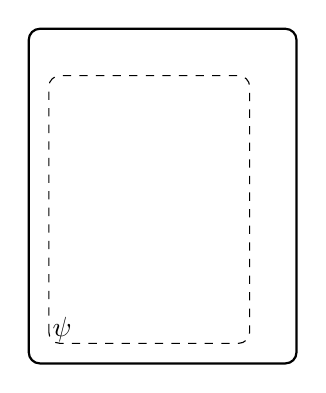
\begin{tikzpicture}[scale=.85]
      \coordinate (epVC) at (0,0);
      \coordinate (epV) at (4,5);
      \coordinate (epVLL) at ($(epVC)-0.5*(epV)$);
      \coordinate (epVUR) at ($(epVC)+0.5*(epV)$);
      \draw[thick, rounded corners] (epVLL) rectangle (epVUR);

      \filldraw (0.5*-3,0.5*-4) node {\(\psi\)};
      \coordinate (psiC) at (-.2,-.2);
      \coordinate (psi) at (3,4);
      \coordinate (psiLL) at ($(psiC)-0.5*(psi)$);
      \coordinate (psiUR) at ($(psiC)+0.5*(psi)$);
      \draw[dashed, rounded corners] (psiLL) rectangle (psiUR);
    \end{tikzpicture}
    \caption{\ref{def:requ:crequ:strcture:psi-not-v}}
    \label{fig:crequ:psi}
  \end{subfigure}
  \hfill
  \begin{subfigure}{0.3\linewidth}
    \begin{tikzpicture}[scale=.85]
      \coordinate (epVC) at (0,0);
      \coordinate (epV) at (4,5);
      \coordinate (epVLL) at ($(epVC)-0.5*(epV)$);
      \coordinate (epVUR) at ($(epVC)+0.5*(epV)$);
      \draw[thick, rounded corners] (epVLL) rectangle (epVUR);

      \filldraw (0,0) node {\(\phi\)};
      \coordinate (phiC) at (-.25,-.25);
      \coordinate (phi) at (2,3);
      \coordinate (phiLL) at ($(phiC)-0.5*(phi)$);
      \coordinate (phiUR) at ($(phiC)+0.5*(psi)$);
      \draw[dashdotted, rounded corners] (phiLL) rectangle (phiUR);

      \filldraw (0.5*-3,0.5*-4) node {\(\psi\)};
      \coordinate (psiC) at (-.2,-.2);
      \coordinate (psi) at (3,4);
      \coordinate (psiLL) at ($(psiC)-0.5*(psi)$);
      \coordinate (psiUR) at ($(psiC)+0.5*(psi)$);
      \draw[dashed, rounded corners] (psiLL) rectangle (psiUR);
    \end{tikzpicture}
    \caption{\ref{def:requ:crequ:strcture:subset} \& \ref{def:requ:crequ:strcture:propersubset}}
    \label{fig:crequ:subset}
  \end{subfigure}
  \hfill
  \begin{subfigure}{0.3\linewidth}
    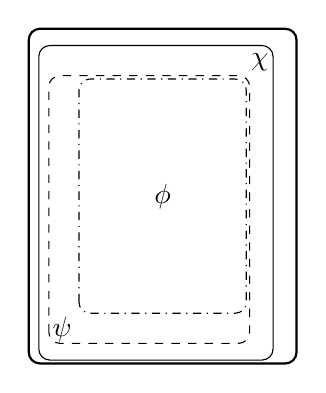
\begin{tikzpicture}[scale=.85]
      \coordinate (epVC) at (0,0);
      \coordinate (epV) at (4,5);
      \coordinate (epVLL) at ($(epVC)-0.5*(epV)$);
      \coordinate (epVUR) at ($(epVC)+0.5*(epV)$);
      \draw[thick, rounded corners] (epVLL) rectangle (epVUR);

      \filldraw (0.5*2.9,0.5*4) node {\(\chi\)};
      \coordinate (chiC) at (-.1,-.1);
      \coordinate (chi) at (3.5,4.7);
      \coordinate (chiLL) at ($(chiC)-0.5*(chi)$);
      \coordinate (chiUR) at ($(chiC)+0.5*(chi)$);
      \draw[rounded corners] (chiLL) rectangle (chiUR);

      \filldraw (0.5*-3,0.5*-4) node {\(\psi\)};
      \coordinate (psiC) at (-.2,-.2);
      \coordinate (psi) at (3,4);
      \coordinate (psiLL) at ($(psiC)-0.5*(psi)$);
      \coordinate (psiUR) at ($(psiC)+0.5*(psi)$);
      \draw[dashed, rounded corners] (psiLL) rectangle (psiUR);

      \filldraw (0,0) node {\(\phi\)};
      \coordinate (phiC) at (-.25,-.25);
      \coordinate (phi) at (2,3);
      \coordinate (phiLL) at ($(phiC)-0.5*(phi)$);
      \coordinate (phiUR) at ($(phiC)+0.5*(psi)$);
      \draw[dashdotted, rounded corners] (phiLL) rectangle (phiUR);
    \end{tikzpicture}
    \caption{Example premise(s)}
    \label{fig:crequ:intuition:prem-ex}
  \end{subfigure}
  \hfill\mbox{ }
  \caption{\crequ{}}
  \label{fig:crequ:intuition}
\end{figure}

\begin{note}[Weaker]
  That \(\psi\) having value \(v'\) is strictly weaker than \(\phi\) having value \(v\) captures an intuitive sense in which whether \(\psi\) has value \(v'\) is an antecedent check on concluding that \(\phi\) has value \(v\) from \(\delta\).

  Further, that \(\psi\) having value \(v'\) is strictly weaker than \(\phi\) having value \(v\) ensures that the definition of a \crequ{} is compatible with granting that concluding any proposition-value pair also \indicateV{} any weaker proposition-value pair.

  For, if \(\phi\) were to have value \(v\) in every \epVW{} for which \(\psi\) has value \(v'\) it would not be possible for the agent to conclude that \(\psi\) has value \(v'\) without the conclusion also \indicateV{} that \(\phi\) has value \(v\).\nolinebreak
  \footnote{
    Note, \ref{def:requ:crequ:strcture:psi-not-v} does not place any constraints on how the premises of the step of reasoning relate to \(\psi\) having value \(v'\) (or \(\phi\) having value \(v\)).
    \autoref{fig:crequ:intuition:prem-ex} depicts a possibility, but in general the agent may entertain arbitrary proposition-value pairs as premises.

    Hence, satisfying the definition of a \crequ{} will not ensure that the step is `reasonable'.
    For example, be that there is no \epVW{} where \(\chi_{1},\dots,\chi_{k}\) all have values \(v_{1},\dots,v_{k}\), and hence the agent would, if they were to conclude \(\phi\) has value \(v\), reason from premise proposition-value pairs that the agent do not consider \epVAd{}.

    Still, \ideaCS{} is only a necessary condition on claiming support, and in turn a \requ{}, and specifically a \crequ{}, need not capture every way in which a step of reasoning may be problematic (with respect to claiming support).

    And, as we will observe, the partner definition of a \prequ{} will place some constraints on when an agent may appeal to some premises to claim support for some conclusion.
  }

  It also follows from both \(\psi\) having value \(v'\) is strictly weaker than \(\phi\) having value \(v\) and the \epVN{} of \(\psi\) not having value \(v'\), that there is some \epVW{} in which \(\phi\) does not have value \(v\).
  In this respect, the definition of a \crequ{} is restricted to non-deductive steps of reasoning.\nolinebreak
  \footnote{
    This is not to deny that the definition of a \requ{} may be extended to cover cases of deductive reasoning.
    Still, it is unclear to me (at least) how the intuitive idea of a \crequ{} \emph{could} be extended to deductive steps.
    For, at issue is whether the agent may have first witnessed some other reasoning which would prevent the agent from concluding that \(\phi\) has value \(v\), but if \(\phi\) having value \(v\) follows deductively, then no other reasoning is possible without the agent having concluded that some proposition has multiple incompatible values, or the agent revising their current epistemic state.

    Still, this is not to deny that an agent may make a non-deductive step of reasoning by appeal to a deductive step.
    For example, the agent may fail to note a key restriction on a theorem before applying it to a specific case.
    However, the distinction between whether a step of reasoning is deductive or non-deductive is made independently of the agent's perspective.
  }
\end{note}


\begin{note}[\ref{def:requ:prequ:no-revision}]
  However, \ref{def:requ:prequ:no-revision} captures an important subtlety regarding the agent's epistemic state that does not reduce to the present relation between various proposition-value pairs.
  For, it may be that the extant relation between \(\phi\) having value \(v\) and \(\psi\) having value \(v'\) is unimportant to the agent.

  Consider a familiar situation from \citeauthor{Harman:1986ux}:

  \begin{quote}
    Mary believes, prior to looking in the cupboard, that if she looks in the cupboard, then she will see a box of Cheerios.
    Mary then looks in the cupboard and does not see a box of Cheerios.
    Hence, Mary abandons her belief about what she would see if she looks in the cupboard.\nolinebreak
    \mbox{}\hfill\mbox{(\citeyear[Cf.][Chs.1\&2]{Harman:1986ux})}
  \end{quote}

  In a similar way, an agent may abandon any relation between the premises of some step and \(\psi\) having value \(v'\) rather than hold that so long as the premises have their respective values then \(\psi\) has value \(v'\).
  For example, an agent may hold that the fire alarm will active whenever there is a fire.
  Though, allow for the possibility that the fire alarm may active when there is no fire.
  However, given the presence of fire with an the appearance of no alarm, the agent may abandon that the fire alarm will active whenever there is fire in order to conclude that someone is in danger, rather than investigating when the alarm really is active.

  In this respect, clause \ref{notion:requ:structure:need-psi} of \autoref{notion:requ} would not be satisfied --- it is \epVAd{} for the agent to conclude that someone is in danger from the presence of fire without being \committed{} to the fire alarm being active.

  While both \ref{def:requ:prequ:strcture} and \ref{def:requ:prequ:no-revision} relate to the same intuitive point, these are separated in the definition of a \prequ{} as \ref{def:requ:prequ:strcture} concerns the structure of the agent's current epistemic state, while \ref{def:requ:prequ:no-revision} concerns a subjunctive property of the present structure.
\end{note}

\subsubparagraph{Relevance}

\begin{note}[Relevance]
  By relativising the core of the constraint to the agent's perspective we ensure that whether or not \(\psi\) has value \(v'\) is relevant to the agent's own reasoning.
  In particular, we ensure that whether or not \(\psi\) having value \(v'\) matters to whether or not \(\chi_{i}\) have values \(v_{i}\) by the agent's own lights, so to speak.

  Variations on the idea of a \prequ{} may take into account the epistemic states of other agents. For example if the agent were engaged in not merely reasoning to, but arguing for, some conclusion.
  Still, for present purposes we only identifying \(\psi\) having value \(v'\) as a \prequ{} if the agent considers it \epVAd{} to `check' their appeal to some premises prior to making a step of reasoning.

  This observation will be important for motivating \ideaCS{} via \ideaS{}.

  For now, observe:

  If \ref{def:requ:prequ:possible-reason} is satisfied, and the agent were to fail to conclude that \(\psi\) has value \(v'\), then the agent would be unable to distinguish an \epVW{} in which \(\psi\) has value \(v'\) and \(\chi_{i}\) have values \(v_{i}\) from an \epVW{} in which \(\psi\) does not have value \(v'\) and \(\chi_{i}\) does not have values \(v_{i}\).
  Hence, it would seem that from the agent's perspective that they have no basis for concluding that \(\phi\) has value \(v\) by appeal to \(\chi_{i}\) having values \(v_{i}\).
\end{note}

\subsubparagraph{The possibility of reasoning}

\begin{note}
  \ref{prequ:int:reasoning} is primarily captured by \ref{def:requ:prequ:possible-reason}.
  However, \ref{def:requ:prequ:possible-reason} is significantly more complex than \ref{prequ:int:reasoning}.

  In order to clarify \ref{def:requ:prequ:possible-reason}, we break down the clause in to three important components, and will discuss each component in turn.
  The three important components are:
  \begin{itemize}
  \item
    First, the core of the constraint concerning reasoning.
  \item
    Second, a relativisation of the core of the constraint to what is \epVAd{} for the agent.
  \item
    Third, a restriction on the scope of the core of the constraint relative to what is \epVAd{} for the agent to \epVW{1} in which the premises are true.
  \end{itemize}
\end{note}

\subsubparagraph{The core constraint}

\begin{note}[Constraint]
  The constraint:
  \begin{quote}
    There is some temporal extension of any relevant \epVW{} in which the agent witnesses reasoning which concludes that \(\psi\) has value \(v'\).
  \end{quote}

  Recall, any (relevant) \epVW{} is a candidate for the actual \world{}.
  And, by temporal extension we mean the progression of a \world{} up to some future point in time.

  So, at core, the constraint specifies that the agent has the opportunity to reason about whether \(\psi\) has value \(v'\), and if the agent were to reason about whether \(\psi\) has value \(v'\), the agent would conclude that \(\psi\) has value \(v'\).

  Note, the core of the constraint only requires that there is \emph{some} temporal extension of any given \epVW{}.
  Hence, the core of the constraint does not require that the agent \emph{will} conclude that \(\psi\) has value \(v'\).
\end{note}

\begin{note}[Delicacy]
  On the one hand it is simple to fail the core of the constraint.
  For, the core of constraint requires that the agent would not fail to conclude that \(\psi\) has value \(v'\).
  On the other hand, it is difficult to fail the core constraint.
  For, the core constraint requires only that there is at least one instance in which the agent would not fail to conclude that \(\psi\) has value \(v'\).

  To illustrate, consider two different kinds of uncertainty.

  On the one hand, and agent may be uncertain about whether they would conclude that \(\psi\) has value \(v'\) due to, say, requiring some information that they may or may not be in a position to acquire.
  If so, then the agent will be unsure about whether there \emph{is} a temporal extension of the relevant \world{}.
  For, the existence of the required temporal extension will depend on whether the agent acquires the required information.
  Hence the core of the constraint will not be satisfied.

  Note, the relevant sense of the copula `is' concerns existence, rather than possibility, however the notion of existence is understood for temporal extensions.

  On the other hand, an agent may be uncertain about whether they really do have the opportunity to conclude that \(\psi\) has value \(v'\) as any instance of reasoning may be interrupted.
  However, so long as there is no guarantee that the agent's reasoning would be interrupted, then the core of the constraint will be satisfied, even if it is highly unlikely that the agent would conclude the relevant reasoning.

  Somewhere between these two extremes is a more nuanced constraint.
  Still, in order to keep the complexity of the constraint (relatively) low, we will not add further conditions.
  In cases where the constraint is to simple to fail, then the definition of a \requ{} may be added to, as \(\psi\) having value \(v'\) being a \prequ{} is only a sufficient condition for \(\psi\) having value \(v'\) being a \requ{}.
  And, we will avoid applying the definition of \prequ{} in cases where the definition exceeds intuition.
\end{note}

\paragraph{Temporal extension}

\begin{note}
  \color{red}
  Need to say more about this.
\end{note}

\begin{note}
  Receiving a letter.
  Unmarked, okay, it's for me.
  Marked, check the address.
\end{note}

\begin{note}[Illustration, testimony]
  To illustrate, consider expert testimony to a layperson.
  Suppose you, the expert, have testified to me, the layperson, that there are exactly five intermediate logics that have the interpolation property.\nolinebreak
  \footnote{Cf.\ \textcite{Maksimova:1977un}}
  From this it follows that there is an intermediate logics that has the interpolation property.
  However, I am quite confident that I would not be in a position to claim support for the latter proposition without your testimony.
  Given that I do not have the expertise involved, any failure by me to claim support that there is a intermediate logic with the interpolation property is uninformative.
  Likewise, given that I am a layperson I'm not in a position to rule out that there aren't intermediate logics with the interpolation property, and therefore I may consider this a potential defeater to your testimony.\nolinebreak
  \footnote{
    Additional example: reports of internal states.

    I have a virus scanner.
    Run this on your pc.
    Also, a test pc.
    Test PC contains a know virus, so if the virus scanner is good, then it will identify infection.
    However, no relation between your PC and my test PC.
    All that would be established is that the scanner is not good for claiming support.
    }

  Still, given \ref{nI:background}, agent may hold that \(\psi\) to have value \(v'\), and may claim support.
  And, may expect to have the resources to claim support for \(\psi\) without appealing to \(\phi\) having value \(v\).
  To illustrate, suppose you and I are both experts.
  You claim to have developed a sound and complete proof system for an logic and presented me with a paper containing the system and a proof.
  Given that I have the paper and the expertise, I am confident that I would be mistaken or misled by your testimony if I am not in a position to claim support that the system is sound and complete by working through the paper.\nolinebreak
  \footnote{
    Here, complexity of understanding of having resources shows.
    For, it may be that the reader learns something new, a lemma etc.\ which could be considered a new resource.
    Likewise, one may think that it's fine to continue to follow testimony given a problematic proof as one is confident that the prover has the resources to revise the proof.
    If so, not clear whether conditional holds, and will depend having resources.
    If proof synthesises resources, then may still hold.
    If proof introduces new information, then conditional does not hold.

    No clear answer for these cases.
    Intend to be compatible with your understanding of resources.
    Will only take a stance on this when applying.
  }
\end{note}

\begin{note}
  Even more difficult
\end{note}

\begin{note}
  Coworker.
  Rely on colleague, as the agent doesn't have access to the file.
  But, access is granted quickly after hearing from the colleague.
\end{note}

\begin{note}
  These cases are harder within the broader context of \nI{}.
  Deny \RBV{}.
  Issue is that in both cases, result seems excessive.

  Well, first thing to do is to check that the agent really is claiming support.
  Fine, it seems, for the agent to stop at claiming support for the other agent, and not going any further.
  See no reason to hold that the agent must claim support.

  Still, this isn't quite satisfactory.
  Doesn't seem that bad, and the above suggestion requires a careful understanding of when an agent is required to claim support.
  So, what if the agent does claim support?

  As noted above, views on testimony can sort this out.
  First, by going for `weak' testimony.
  Second, by breaking \ref{nI:inclusion:bound} is the testimony turns out to be a mistake.
  Look, it's not obvious why it would make sense for the agent to claim support, but the point is that \nI{} wouldn't hold.

  Alternatively, Simple restriction is for first time claiming of support.
  Difficulty is a variation of the expert case.
  It isn't obvious that one gets to claim support for the stuff learnt as a layperson when one develops expertise.
  For example, translation between languages.
  Claim support for simple translation.
  When fluent, seems claimed support is distinct, based on broader understanding of the language.
  Not relying on simplifications in learner's dictionary.

  However, other ways of claiming support may also work.
  Arguing for one such way.
  Besides this, \RBV{} is quite strong.
  And, who knows about other types of reasoning.
  In particular, ways in which reasoning \adA{} might work.
\end{note}

\begin{note}[Uninspiring]
  These responses aren't particularly inspiring.

  However, let's look at this from a different angle.
  What's going to follow from insensitivity to context?
  End up with claiming support that does not depend on whether or not the agent is in a position to deal with defeaters.

  Well, the first option is that these never matter.

  Some kind of built in support.
  This comes up with ~\citeauthor{Pryor:2012tq}'s dogmatism (\cite{Pryor:2000tl,Pryor:2012tq}) and various ideas about entitlement (Wright, Burge, etc.)
  For example, Pryor's dogmatism for perception, just having the experience is good enough.
  Question about these kinds of defeaters.
  Reads to me that these kinds of things mean that \ref{nI:inclusion} will never hold.

  Question is whether this extends to all cases, so that \nI{} is trivial, but before pressing this seems too strong.
  Problems in various cases.
  The red room, but in the corner is a switch, flipped to off, but says it's broken.

  Context makes a difference.
  So, to this extent, looks as though there's going to be difficult cases.
\end{note}

\begin{note}[Following doesn't depend on difficult cases]
  Of course, this isn't a general defence of the clauses.
  Rather, that such difficulties can't be avoided.
  Upshot here is that we aren't really interested in such difficult cases.
\end{note}

\subsubparagraph{The role of the agent}

\begin{note}
  Our discussion of the core of the constraint focused on there being some temporal extension of the \world{} in which \vAgent{} witnesses reasoning which concludes that \(\psi\) has value \(v'\).

  In general, whether or not the core of the constraint is satisfied by be evaluated independently of the agent's perspective on how the actual \world{} is.
  Still, we relativise the core of the constraint to the agent's perspective.

  The motivation is simple and has two (related) parts.
  \begin{itemize}
  \item
    First, we ensure that \(\psi\) having value \(v'\) is relevant to the agent's reasoning.
  \item
    Second, we reduce latent issues concerning whether there is some temporal extension of a \world{} to an single source --- the agent.
  \end{itemize}
  We expand on both points in turn.
\end{note}

\subsubparagraph{Latent issues}

\begin{note}
  The upshot of resolving the relevant sense of possibility to the agent's epistemic state is that we avoid questions about whether it is possible for an agent to recognise that it is possible for them to conclude that \(\psi\) has value \(v'\).
  For, if it is \epVAd{} for the agent to witness reasoning which concludes that \(\psi\) has value \(v'\), then the agent holds that for every candidate for the actual \world{}, there is some extension of the candidate \world{} in which the agent witnesses the relevant reasoning.\nolinebreak
  \footnote{
    Note, this does not guarantee that the agent would witness reasoning which concludes that \(\psi\) has value \(v'\) if the agent were to try, as we do not require that the actual \world{} is always an \epVW{}.
  }

  For example, it may be `possible' for the agent to conclude that the liquid in a glass is not poisoned prior to appealing to it being safe to drink in order to conclude that they should drink the liquid.

  In order to resolve whether it really is possible the agent to conclude that the liquid in a glass is not poisoned, we need only consider whether the agent considers it \epVAd{} that they may witness such reasoning.
  And, the answer may be negative as the agent expects dehydration to set in before concluding any such reasoning.
\end{note}

\begin{note}
  The upshot comes with a corresponding downshot.
  For, it may be possible (in the relevant intuitive sense) for the agent to witness reasoning which concludes that \(\psi\) has value \(v'\) without the agent holding that it is \epVAd{} for them to so reason.

  For example, it may be possible (and quite straightforward) for an agent to check the boiler for a simple fault before appealing to the premises that it is broken in order to conclude that they should call for a repair.
  Yet, so long as the agent does not consider it \epVAd{} for them to check the boiler, any proposition-value pair captured a simple fault will not be a \prequ{}.
\end{note}

\subsubparagraph{Quantification}

\begin{note}
  Finally we turn restricting the scope of the core of the constraint to \epVW{1} in which all of the premises that the agent would appeal to when making the step of reasoning have the appropriate values.

  Key here is that the core of the constraint requires that there is some temporal extension of the relevant \epVW{1} in which the agent witnesses reasoning which concludes that \(\psi\) \emph{has} value \(v'\).

  This gives rise to the following problem:
\end{note}

\begin{note}[Problem]
  In order for \(\psi\) having value \(v'\) to be a \crequ{} the agent must consider it \epVAd{} that \(\psi\) does not have value \(v'\).
  Yet, if \(\psi\) does not have value \(v'\), then it may be the case that the agent would fail to conclude that \(\psi\) has value \(v'\).\nolinebreak
  \footnote{
    In particular, whether \(\psi\) has value \(v'\) may be straightforwardly decidable for the agent, and hence if the agent were to reason about whether \(\psi\) has value \(v'\) and \(\psi\) does not have value \(v'\), then they agent would conclude that \(\psi\) does not have value \(v'\).
  }
  In which case, the core of the constraint will fail to be satisfied.
\end{note}

\begin{note}[Solution]
  \color{red}
  Still, quantifying over \epVW{1} in which \(\phi\) has value \(v\) provides a motivated solution.

  For, we are only interested in the idea \(\psi\) having value \(v'\) being \crequ{} as a check on whether it would make sense for an agent to conclude that \(\phi\) has value \(v\) from a collection of premises.
  Hence, in order for the \crequ{} to be a check of the relevant kind, we are only interested in cases where the agent would (`successfully') make the step.

  In other words, the agent is moving to \(\phi\), and so long as this would make sense, it says something about what the agent can do.
  It does not need to follow that the agent can reason to \(\psi\) in general.

  Therefore, we may restrict the interest in the possibility of concluding that \(\psi\) has value \(v'\) to those \epVW{1} in which \(\phi\) has value \(v\).
\end{note}

\begin{note}[Illustration]
  To illustrate.

  \begin{illustration}
    Suppose an agent wishes to conclude that a parcel has gone missing from the premise that they are not (yet, at least) in possession of the parcel.

    If the parcel has gone missing, then no delivery attempt will have been made, and no note will be on their front door.
    Still, if the parcel has \emph{not} gone missing, then a delivery may have been attempted, and a note left on the agent's front door.
    And, the agent considers it \epVAd{} that a delivery was attempted earlier in the day, and that a note was left on their front door.
  \end{illustration}

  Premise, that the agent is not in possession of the parcel.
  Conclusion, the parcel has gone missing.

  However, check.
  That no delivery has been made.

  If the parcel is missing, then no note.

  So, satisfy the core of the constraint in the case of missing.

  However, if the parcel has not gone missing, there may be a note.
  So, failure to satisfy the core of the constraint in the case of not missing.
\end{note}

\begin{note}
  Key is that if not, then expect failure.
\end{note}

\paragraph{Motivation from \support{}}

\begin{note}
  We now turn to motivating \ideaCS{} with respect to \prequ{1}.
\end{note}

\begin{note}
  If the agent has not concluded for each of the premises, then it's at least necessary that conclude for \(\psi\).
  For, if not, then if were to reason about \(\psi\), then might go to \(\lnot\psi\).
  Hence, that the premises do not jointly hold.
  Therefore, the premises are not a \sink{}, and \(\phi\) is not a \sink{}.
\end{note}

\begin{note}
  There are two exceptions.

  First, that it is not possible for the agent to reason.
  Without this, then no failure of being a \sink{}.

  Second, giving up whatever leads to \(\psi\) being a \prequ{}.
  This is because the definition of a \prequ{} does not rely on the agent recognising that \(\psi\) is a \prequ{}.
  Hence, possibility that agent may revise their epistemic state to avoid \(\psi\) being a \prequ{}.
  Simply done by abandoning any link.
\end{note}

\begin{note}[\prequ{}]
  \prequ{}.
  Then, premises of \(\delta\) do not hold with respect to all \epVW{1}.
  And, there is some way for the agent to reason.
  Problem here is quite clear.
  Question is whether something stronger.
  This depends on possibility of reasoning.
  If general, then simplifies.
  Reasoning for anything by required by premises.
  If not, then \(\psi\) falls outside of our interest.
  \support{2} is just about reasoning.
\end{note}



\paragraph{\illu{3} of \crequ{1}}

\begin{note}
  Key is to find a series of necessary conditions for some conclusion.
\end{note}

\subparagraph{Where's Wally}

\begin{note}
  Back to initial \illu{0}.
\end{note}

\begin{note}
  Problem.
  \requ{}.
  Agent didn't notice, so possibility.
  And, agent is appealing to it being Wally.
  Not merely that they identified as Wally.

  It's not clear need to give up claimed support, but does not extend to having a cane.

  In contrast to \ref{illu:CS:spot-the-diff}, does not seem there is anything weaker to fall back on.
  However, no strong claim here.
  Rely on stronger principles about claiming support.
\end{note}

\subparagraph{Spot the difference}

\begin{note}[Spot the difference]
  \begin{illustration}[Spot the difference]
    \label{illu:CS:spot-the-diff}
    The agent has been working through a spot-the-difference to pass some time.

    Though the time is not completely passed, the agent examined the two images with what seems sufficient care to claim support that they have found all the differences.
    However, the agent did not keep track of the number of differences.

    The agent announces `I have found all the differences' and their companion responds `All fifteen?'.

    \begin{enumerate}[label=\arabic*., ref=(I\ref{illu:CS:spot-the-diff}.\arabic*)]
      \setcounter{enumi}{-1}
    \item
      \label{illu:CS:spot-the-diff:info}
      If I have found all the differences, I have found fifteen differences.
    \end{enumerate}

    The agent then reasons as follows:

    \begin{enumerate}[label=\arabic*., ref=(I\ref{illu:CS:spot-the-diff}.\arabic*), resume]
    \item Exhaustive search.
    \item
      \label{illu:CS:spot-the-diff:all}
      I found all the differences.
    % \item\label{illu:CS:spot-the-diff:info} My companion has testified that there are fifteen differences.
    % \item\label{illu:CS:spot-the-diff:cond} If I have found all the differences, I have found fifteen differences.
    \item
      \label{illu:CS:spot-the-diff:fif}
      So, I have found fifteen differences. \hfill (From \ref{illu:CS:spot-the-diff:info} and \ref{illu:CS:spot-the-diff:all})
    \end{enumerate}
  \end{illustration}

  Before going further, structure of this.

  The agent performed some reasoning, and concluded that they found all the differences.
  However, that reasoning is mentioned but not stated in the \illu{0}.
  Rather, present is distinct instance of reasoning after being provided with information.
  ``If not 15, then problem''.
  Present reasoning appeals to past reasoning, and draws out consequence of this given new information.
  Important: the present reasoning does not consider possibility that the agent did not find all 15 differences.
  Instead, consequence of conclusion of previous instance of reasoning.
  Still, epistemically possible that the agent did not find 15 differences.
\end{note}

\begin{note}
    Providing additional information about what the agent has claimed support for.
  Recall, \autoref{assu:CSVP}, information rather than \world{}.
  \nolinebreak
  \footnote{
    Still slight issue.
    Offering a redescription.
    You met Clark Kent, so you met Superman.
    In this case, rather than claiming support for meeting Superman, provided information is seen as an equivalent formulation.
    It is possible to read \autoref{illu:CS:spot-the-diff} in this way, and this might be the most natural interpretation.
    However, it is not the interpretation under which see the problem.
    Rather, problem is where the conditional is explicit.
    Unlike Superman case, proper conditional.
  }
\end{note}

\begin{note}
  Information leads to \requ{}.

  Possibility of not fifteen.
  And, not merely that the agent performed the reasoning, but that the reasoning identified all.
  If not fifteen, then not all, so would involve appeal to something that is not the case.

  And, present reasoning does not include reasoning about \requ{}.
\end{note}

\begin{note}[Avoiding the problem]
  This doesn't rule out some additional reasoning.
  \begin{enumerate}
  \item Exhausted search.
  \end{enumerate}
  Difference here is that the agent is not only appealing to having found.
  In addition, what they recall about reasoning.
  What matters is not that found all but rather that exhaustivity of search.
  This is not specific to 15.
  Up to some \(k\) such that agent is still confident that they performed an exhaustive search.

  Whether you think this is enough is up to you.
  On the one hand, intuitive that this does enough.\nolinebreak
  \footnote{
    Indeed, reasoning framed with all as I think it is much less clear here.
  }

  On the other hand, the agent did not keep track of the number of differences.
  So, may hold that they should go back and count.\nolinebreak
  \footnote{
    Looking ahead, \nI{}.
    Difficulty here is that don't need to go to \(\phi\).
    Indeed, note somewhere that \nI{} really only clearly takes hold when need some sort of factivity in play.
    We'll return to this.
  }

  {
    \color{red} As observed in the footnote above, the trick here is that the agent doesn't really `need' to go to having found all the differences.

    Alternatively, not enough to show that the reasoning is bad.
    E.g.\ then I would have been deceived, some trick, etc.
    Something \emph{I} wouldn't count as a difference.
  }
\end{note}

\begin{note}
  Argued above against circularity.
  Here, additional consideration.

  If the agent were to have had the information first time, then plausibly an instance of circularity.
  And, may think that this is also circularity as must also all must amount to fifteen.
\end{note}


\subparagraph{Zebra}

\begin{note}
  This is somewhat tentative.
  If you think that you would succeed in checking, then go for it.
\end{note}

\paragraph{Conditionals}

\begin{note}
  \color{red}
  The point of this section should be to note how \ideaCS{} relates to conditionals.
  In the case of truth-functional conditionals, things are quite straightforward.
  In the case of non-truth-function conditionals, not so much.
\end{note}

\begin{note}
  \(\phi \rightarrow \psi\), \(\lnot\psi \rightarrow \lnot\phi\), \(\psi \not\rightarrow \phi\).
  These are the key things.
  Does not extend to probability, because then don't get the overlapping relations.
\end{note}

\subsubparagraph{Closing}

\begin{note}
  Now, taxing.
  Very many things that could be checked.
  But whether an agent has claimed \support{} is not (necessarily) transparent.
  Rather, whether there's a clear problem.
\end{note}

\hozline


\subsubsection{\crequ{3}???}

\begin{note}
    \color{red}
    Note, focus on what the actual world is is important for the second clause.
    If it doesn't matter what the actual world is, then it's hard to see why this would matter.

    `Possible' should be restricted in some way.
    This is also why recursive in the case of \support{} is useful.
    Though, also should state that it's reasoning, with no further information.

    \requ{} is split into two cases.

    \ref{def:requ:crequ} observes that the result of making the step is a conclusion that \(\phi\) has value \(v\) only if \(\psi\) has value \(v'\).
    Alternatively, a conclusion that \(\phi\) has value \(v\) \emph{given} that \(\psi\) has value \(v'\).

    \ref{def:requ:prequ} observes that the premises appealed to cover all \epVW{1} only if \(\psi\) has value \(v'\).
\end{note}

\begin{note}[Intuition for \ideaCS{}]
  \ideaCS{}.
  The notion of a \requ{} specifies how \(\psi\) not having value \(v'\) is involved with step.
  Required in order to make step.
  Then, the problem is that the step will only conclude that \(\phi\) has value \(v\) with respect to a restriction of \world{1} which are \epVAd{} for the agent.
  The agent may conclude that \emph{if} \(\psi\) has value \(v'\), \emph{then} \(\phi\), but as \(\psi\) may not have value \(v'\), the agent may not conclude that \(\phi\) has value \(v\) alone.

  In other words, if an agent is \committed{} to it being that case that some step of reasoning in informative about the actual \world{} \emph{just in case} some proposition \(\psi\) has value \(v\), then unless the agent has witnessed some reasoning which \indicateV{1} that \(\psi\) has value \(v'\), then the step only applies to a restricted collection of \epVW{1}.
\end{note}

\begin{note}[Dynamics]
  Stated in this way, \ideaCS{} is perhaps intuitive.

  The delicate part of \ideaCS{} is dynamics.
  In the cases of interest, the agent has concluded that \(\chi_{i}\) have values \(v_{i}''\) from some prior reasoning, which have satisfied claiming support.
  However, between concluding that \(\chi_{i}\) have values \(v_{i}''\) and reasoning from \(\chi_{i}\) have values \(v_{i}''\) to \(\phi\) having value \(v\), \(\psi\) (not) having value \(v'\) is introduced as an \epVN{}.

  This is where \ideaCS{} will do significant work.
\end{note}

\begin{note}[Relying]
  First, a subtle, but important, distinction is that the reasoning must \emph{rely} on the relevant step.
  Intuitively, some instance of reasoning which concludes that \(\phi\) has value \(v\) relies on a step of reasoning just in case the reasoning requires both the premises and conclusion of the step to actually have their respective values in order to conclude that \(\phi\) has value \(v\).

  In other words, \ideaCS{} does not extend to steps made where the step is part of some hypothetical reasoning, such as reasoning by cases.
\end{note}

\begin{note}[Intuition for \requ{}]
  Key is that \(\psi\) having value \(v'\) is required to make the step.

  ??, ensures that \(\psi\) not having value \(v'\) is relevant to making the step.
  There is not requirement that agent reasons about arbitrary \epVAd{} propositions.
  With respect to \ideaCS{}, keep things simple.
  Though, when defining a \requ{} in ???, strengthen somewhat.

  ??, reduces issues concerning the step to premises and conclusion of the step.

  ??, expands with respect to the agent's epistemic state.
  The use of the term `\committed{}' is to surpass any form of recognition.
\end{note}

\begin{note}
  Of course, it may be that the agent has \support{}.
  However, the reasoning would performed would not be suitable.
  Hence, failure of \emph{claiming} \support{}.

  Following \ideaS{}, \(\phi\) having value \(v\) is not a \sink{} with respect to \epVW{1}.
  Alternatively, it is not clear that the agent concludes that \(\phi\) has value \(v\).
\end{note}

\paragraph{\illu{3}}

\begin{note}
  Some \illu{1}.
  Three \illu{1}.
  In each, reasoning which fails to satisfy \ideaCS{}, then suggested reasoning that would satisfy.
\end{note}

\begin{note}
  Observe, however, that the intuitive problem is not that the agent has any reason(ing) to think that \nagent{11} is \emph{not} trustworthy when speaking on matters regarding their personal character.

  Rather, the intuitive problem is that the agent does not have any reason(ing) to think that \nagent{11} \emph{is} trustworthy when speaking on matters regarding their personal character.

  In particular, that that \nagent{11} is not trustworthy when speaking on matters regarding their personal character is simply a possibility.
  It may be the case that \nagent{11} is trustworthy.\nolinebreak
  \footnote{
    \color{red}
    It's not like this suggests that they are not trustworthy.
    Asking for directions.
    These are fine, but addition is not.
  }
\end{note}

\subsection{Limitations}
\label{sec:limitations}

\begin{note}
  Goal of this section is to argue that \ideaCS{} does not over-generate.
\end{note}

\begin{note}
  The basic point is that while \(\psi\) is a consequence of \(\phi\), it's also the case that \(\phi\) is stronger.
  And, that the agent doesn't need to establish something so strong.
\end{note}

\begin{note}
  The bag contains green balls.
  The bag does not contain any red balls.

  Well, possible to empty the bag.

  However, \crequ{} doesn't cover this case, because the latter is not strictly weaker than the former.
\end{note}

\begin{note}
  X has at least \(\$100\).
  Well, then, X has at least \(\$1\), etc.

  Here, something nested.
  Where, it's always possible to check something weaker.

  It's hard to think of a compelling case.
  Still, the structure should be clear.

  Now, this does not mean that it is not possible for an agent to conclude some intermediary without previous.
  For, what the agent appeals to for an intermediary may also cover previous.
  Saw with \(\$50\), and this \indicateV{} \(\$50 - x\).

  What matters is that there's some jump, and an antecedent check on whether that jump makes sense that the agent hasn't considered.
  Yet \(\$50\) clearly works for all previous checks.
\end{note}

\subsection{\prequ{3}}
\label{sec:prequ3}

\begin{note}
  Definition of a \requ{} focused on particular structure.
  However, only a sufficient condition.
  Here, we consider \prequ{}.
  Observe this places further constraints.
  However, stronger.
  Any \prequ{} is a \crequ{}.
  Note, however, vice-versa.
\end{note}

\paragraph{Definition}

\begin{definition}
  \label{def:requ:prequ}
  \(\psi\) having value \(v'\) is a \emph{\prequ{}} of \(\delta\) \emph{if and only if} the following conditions jointly hold:
  \begin{enumerate}[label=\arabic*., ref=\named{P\(\Re\):\arabic*}]
  \item
    \label{def:requ:prequ:strcture}
    The structure of the \vAgent{}' epistemic state is such that:
    \begin{enumerate}[label=\alph*., ref=\named{P\(\Re\):1\alph*}]
    \item
      \label{def:requ:prequ:strcture:psi-not-v}
      There is some \epVW{} such that:
      \begin{itemize}
      \item
        \(\psi\) does not have value \(v'\).
      \end{itemize}
    \item
      \label{def:requ:prequ:strcture:chi-subset-psi}
      There is no \epVW{} such that:
      \begin{itemize}
      \item
        \(\chi_{i}\) have value \(v_{i}\) and \(\psi\) does not have value \(v'\)
      \end{itemize}
    \item
      \label{def:requ:prequ:strcture:chi-propersubset-psi}
      There is some \epVW{} such that:
      \begin{itemize}
      \item
        \(\psi\) has value \(v'\) and some \(\chi_{i}\) does not have value \(v_{i}\).
      \end{itemize}
    \end{enumerate}
  \item
    \label{def:requ:prequ:no-revision}
    It is not the case that the agent would revise their epistemic state so that \ref{def:requ:prequ:strcture:chi-subset-psi} does not hold (in order to conclude that \(\phi\) has value \(v\) from \(\delta\)).
  \item
    \label{def:requ:prequ:possible-reason}
    For all \epVW{} in which \(\chi_{i}\) have values \(v_{i}\), there is some temporal extension of the \world{} in which \vAgent{} witnesses reasoning which concludes that \(\psi\) has value \(v'\).
  \end{enumerate}
\end{definition}

\paragraph{Idea}

\begin{note}
  Intuitively, \(\psi\) having value \(v'\) is a \prequ{} of some step of reasoning just in case:
  \begin{enumerate}[label=\arabic*., ref=(\arabic*)]
  \item
    \label{prequ:int:structure}
    \(\psi\) not having value \(v'\) is \epVAd{} and the relevant \emph{premise} proposition-value pairs of the step are paired only if \(\psi\) has value \(v'\), and
  \item
    \label{prequ:int:reasoning}
    It is possible, given the agent's epistemic state, for the agent to conclude that \(\psi\) has value \(v'\) prior to making the step of reasoning.
  \end{enumerate}
\end{note}

\paragraph{The structure}

\begin{note}
  \ref{prequ:int:structure} is primarily captured by \ref{def:requ:prequ:strcture}, where:

  \ref{def:requ:prequ:strcture:psi-not-v} ensures that \(\psi\) may not have value \(v'\).
  And, \ref{def:requ:prequ:strcture:chi-subset-psi} together with \ref{def:requ:prequ:strcture:chi-propersubset-psi} ensure that the \world{1} in which the premise proposition-value pairs holds are a subset (from \ref{def:requ:prequ:strcture:chi-subset-psi}) and moreover a \emph{proper} subset (from \ref{def:requ:prequ:strcture:chi-propersubset-psi}) of the \world{1} in which \(\psi\) has value \(v'\).

  \begin{figure}
    \mbox{ }\hfill
    \begin{subfigure}{0.3\linewidth}
      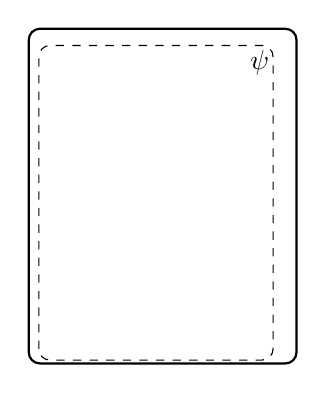
\begin{tikzpicture}[scale=.85]
        \coordinate (epVC) at (0,0);
        \coordinate (epV) at (4,5);
        \coordinate (epVLL) at ($(epVC)-0.5*(epV)$);
        \coordinate (epVUR) at ($(epVC)+0.5*(epV)$);
        \draw[thick, rounded corners] (epVLL) rectangle (epVUR);

        \filldraw (0.5*2.9,0.5*4) node {\(\psi\)};
        \coordinate (psiC) at (-.1,-.1);
        \coordinate (psi) at (3.5,4.7);
        \coordinate (psiLL) at ($(psiC)-0.5*(psi)$);
        \coordinate (psiUR) at ($(psiC)+0.5*(psi)$);
        \draw[dashed, rounded corners] (psiLL) rectangle (psiUR);
      \end{tikzpicture}
      \caption{\ref{def:requ:prequ:strcture:psi-not-v}}
      \label{fig:prequ:intuition:psi-not-v}
    \end{subfigure}
    \hfill
    \begin{subfigure}{0.3\linewidth}
      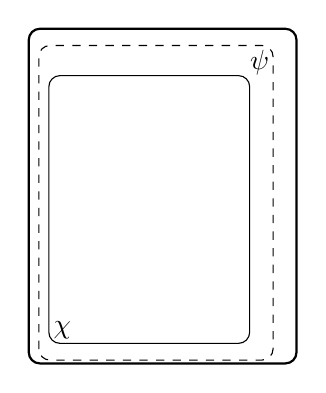
\begin{tikzpicture}[scale=.85]
        \coordinate (epVC) at (0,0);
        \coordinate (epV) at (4,5);
        \coordinate (epVLL) at ($(epVC)-0.5*(epV)$);
        \coordinate (epVUR) at ($(epVC)+0.5*(epV)$);
        \draw[thick, rounded corners] (epVLL) rectangle (epVUR);

        \filldraw (0.5*2.9,0.5*4) node {\(\psi\)};
        \coordinate (psiC) at (-.1,-.1);
        \coordinate (psi) at (3.5,4.7);
        \coordinate (psiLL) at ($(psiC)-0.5*(psi)$);
        \coordinate (psiUR) at ($(psiC)+0.5*(psi)$);
        \draw[dashed, rounded corners] (psiLL) rectangle (psiUR);

        \filldraw (0.5*-3,0.5*-4) node {\(\chi\)};
        \coordinate (chiC) at (-.2,-.2);
        \coordinate (chi) at (3,4);
        \coordinate (chiLL) at ($(chiC)-0.5*(chi)$);
        \coordinate (chiUR) at ($(chiC)+0.5*(chi)$);
        \draw[rounded corners] (chiLL) rectangle (chiUR);
      \end{tikzpicture}
      \caption{\ref{def:requ:prequ:strcture:chi-subset-psi} \& \ref{def:requ:prequ:strcture:chi-propersubset-psi}}
      \label{fig:prequ:intuition:subset}
    \end{subfigure}
    \hfill
    \begin{subfigure}{0.3\linewidth}
      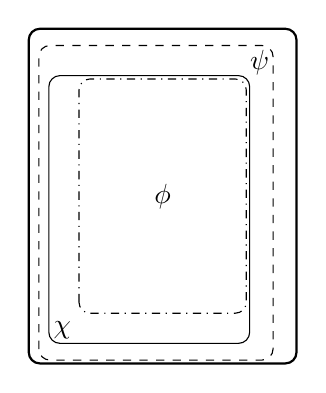
\begin{tikzpicture}[scale=.85]
        \coordinate (epVC) at (0,0);
        \coordinate (epV) at (4,5);
        \coordinate (epVLL) at ($(epVC)-0.5*(epV)$);
        \coordinate (epVUR) at ($(epVC)+0.5*(epV)$);
        \draw[thick, rounded corners] (epVLL) rectangle (epVUR);

        \filldraw (0.5*2.9,0.5*4) node {\(\psi\)};
        \coordinate (psiC) at (-.1,-.1);
        \coordinate (psi) at (3.5,4.7);
        \coordinate (psiLL) at ($(psiC)-0.5*(psi)$);
        \coordinate (psiUR) at ($(psiC)+0.5*(psi)$);
        \draw[dashed, rounded corners] (psiLL) rectangle (psiUR);

        \filldraw (0.5*-3,0.5*-4) node {\(\chi\)};
        \coordinate (chiC) at (-.2,-.2);
        \coordinate (chi) at (3,4);
        \coordinate (chiLL) at ($(chiC)-0.5*(chi)$);
        \coordinate (chiUR) at ($(chiC)+0.5*(chi)$);
        \draw[rounded corners] (chiLL) rectangle (chiUR);

        \filldraw (0,0) node {\(\phi\)};
        \coordinate (phiC) at (-.25,-.25);
        \coordinate (phi) at (2,3);
        \coordinate (phiLL) at ($(phiC)-0.5*(phi)$);
        \coordinate (phiUR) at ($(phiC)+0.5*(chi)$);
        \draw[dashdotted, rounded corners] (phiLL) rectangle (phiUR);
      \end{tikzpicture}
      \caption{Prospective conclusion}
      \label{fig:prequ:intuition:conclusion}
    \end{subfigure}
    \hfill\mbox{ }
    \caption{
      The structure of an agent's epistemic state with respect to \epVW{} when \ref{def:requ:prequ:strcture} is satisfied.
    }
    \label{fig:prequ:intuition}
  \end{figure}
  This structure is depicted in \autoref{fig:prequ:intuition}:

  \begin{itemize}
  \item
    \autoref{fig:prequ:intuition:psi-not-v} represents the agent's epistemic state (the bold rectangle) being such that there are some \world{1} such that \(\psi\) has value \(v'\) (those within the dashed rectangle), and that there are some \world{1} such that \(\psi\) does not have value \(v'\) (those outside the dashed rectangle).
  \item
    \autoref{fig:prequ:intuition:subset} represents the \world{1} in which the collection of premises \(\chi_{i}\) all have respective values \(v_{i}\) are a proper subset of the \world{1} such that \(\psi\) has value \(v'\).
  \item
    \autoref{fig:prequ:intuition:conclusion} represents a prospective conclusion, in which \(\phi\) having value \(v\) is obtained via a non-deductive step of reasoning from \(\chi_{i}\) having values \(v_{i}\), though the relevant step may also be deductive.
  \end{itemize}
\end{note}

\paragraph{\illu{3}}



\begin{note}
  \begin{illustration}
    Computer, not turning on.
    Broken.
    Check that it's plugged in.
  \end{illustration}
\end{note}

\begin{note}
  \begin{illustration}
    Sent documents.
    Up to date.
    Revised at the end of financial year, past that.
    Well, at least check the year of the document.
  \end{illustration}
\end{note}

\begin{note}
  Given the constraints, we mostly get variations on this kind of case.
  The purpose of a \prequ{} is just clarify how to refine the notion of a \requ{}.
  In particular, some of the limitations.
\end{note}

\paragraph{Not completely trivial}

\begin{note}
  Trivially satisfied if the agent has concluded for each of the premises.
  For, given that \(\psi\) is strictly weaker than the premises, any reasoning for the premises is going to \indicateV{} that \(\psi\).

  In this respect, fault is local to the reasoning, and again motivation for broadening to subjunctive considerations regarding relaxing and agent's epistemic state.

  Final: Not completely trivial.
  For, it may be the case that it is not possible for the agent to reason to one of the premises, but that \(\psi\) is still a condition that they could reason to.
\end{note}

\begin{note}
  \begin{illustration}
    The clock is working.
    Without any other source for the time, there's nothing to be done.
    However, it should definitely be ticking.
    Therefore, at the very least check this.
  \end{illustration}
  Or, that it's not clearly daylight outside.

  Not here that it's not clear that the clock would be particularly good.
  However, with respect to constraints, it's fine.
\end{note}

\newpage

\subsection{Contrasts}
\label{sec:contrasts}

\paragraph{Circularity}

\begin{note}
  \ideaCS{} is not about circular reasoning in the sense that the term `circularity' suggests that the reasoner has taken the conclusion of the reasoning for granted.

  There's nothing in \ideaCS{} that appeals to getting \(\psi\) having value \(v'\) from \(\phi\) having value \(v\).

  However, does identify a problem in the sense that would prevent the agent from getting \(\psi\) having value \(v'\) from \(\phi\) having value \(v\).
\end{note}

\begin{note}[Testimony 1]
  \begin{illustration}[Testimony 1]
    \label{illu:CS:test:basic}
    \mbox{}
    \begin{enumerate}[label=\arabic*., ref=(\arabic*)]
    \item
      \label{ex:eiS:t:basic:test}
      \nagent{11} stated that they are trustworthy when speaking on matters regarding their personal character.
    \item
      \label{ex:eiS:t:basic:ok}
      \nagent{11} is trustworthy when speaking on matters regarding their personal character.
    \end{enumerate}
  \end{illustration}
  This kind of case is intuitively problematic.
  It seems that already need trustworthy.
  If this assumption is made, then a problem.
  However, nothing that requires that this assumption is made.
  Therefore, \ideaCS{} does not necessarily identify anything problematic.

  This contrasts to the other \illu{1}, in which the agent is making an a non-deductive step of reasoning.
  What we're interested in is overlooking certain things.

  Indeed, \autoref{illu:CS:test:basic} is difficult because different substitutions seem fine.
\end{note}

\paragraph{Sgaravatti}

\begin{note}
  For example, consider what \citeauthor{Sgaravatti:2013wu} terms the `Justification Account' of circularity.\nolinebreak
  \footnote{
    As \citeauthor{Sgaravatti:2013wu} notes, the Justification Account of circularity is a rewriting of the third type of `epistemic dependence' considered by \citeauthor{Pryor:2004ws}~(\citeyear[359]{Pryor:2004ws}).
    Neither \citeauthor{Pryor:2004ws} nor \citeauthor{Sgaravatti:2013wu} endorse the Justification Account, but I take the spirit of the account to sufficient for interest.
    Still, the considerations which follow also apply to distinguish the {\color{red} problem identified} from \citeauthor{Sgaravatti:2013wu}'s favoured account (\Citeyear[\S3]{Sgaravatti:2013wu}) and the fifth type of `epistemic dependence' considered by \citeauthor{Pryor:2004ws}~(\citeyear[359]{Pryor:2004ws}).
  }

  \begin{quote}
    \begin{enumerate}[label=(JA), ref=(JA)]
    \item\label{sg:JA} An argument is circular if and only if for you to have justification to believe the premisses, it is necessary that you have justification to believe the conclusion.\nolinebreak
      \mbox{}\hfill\mbox{(\Citeyear[754]{Sgaravatti:2013wu})}
    \end{enumerate}
  \end{quote}
  Where `justification to believe' is to be read as in terms of having formed the belief in an epistemically appropriate way as opposed to (merely) possessing sufficient resources to form formed the belief in an epistemically appropriate way.\nolinebreak
  \footnote{
    Or, however you prefer to characterise \citeauthor{Firth:1978vi}'s (\Citeyear{Firth:1978vi}) distinction between doxastic and propositional justification (or warrant).
    See also \citeauthor{Silva:2020aa} (\Citeyear{Silva:2020aa}) --- esp.\ fn.\ 1.
  }
  (\citeauthor[Cf.][754--755]{Sgaravatti:2013wu})
\end{note}

\begin{note}
  First, reliance on something like justification.

  With \support{}, we arguably have something distinct.
  Have not placed constraints on reasoning.
  Hence, \ideaCS{} applies even when no justification (or any other epistemic attribute) is found.

  Indeed, to the extent that the value \(v\) need not be truth, \ideaS{} and \ideaCS{} are broader.

  Point extends to relation between the premises and the conclusion of a step of reasoning.
  There's some issue with whether there's a clear reduction to premises.

  Now, both these points may be addressed by linking justification to steps of reasoning.
  However, it still remains that get this kind of circularity by placing a constraint on permissible steps of reasoning.
\end{note}

\paragraph{Pryor}

\begin{note}[\citeauthor{Pryor:2004ws}'s Type 4]
  An instance of a limitation arising from assuming that the possibility obtains is the fourth type of dependence between premise and conclusion considered by \citeauthor{Pryor:2004ws}.

  \begin{quote}
    [Type 4] dependence between premise and conclusion is that the conclusion be such that evidence \emph{against it} would (to at least some degree) undermine the kind of justification you purport to have for the premises.\nolinebreak
    \mbox{}\hfill\mbox{(\citeyear[359]{Pryor:2004ws})}
  \end{quote}

  Again, plausible.\nolinebreak
  \footnote{
    A variant of \citeauthor{Pryor:2004ws}'s Type 4 dependence is~\citeauthor{Jackson:1984vk}'s account of circularity.
    \begin{quote}
      [I]t may be that a given argument to a given conclusion is such that anyone --- or anyone sane --- who doubted the conclusion would have background beliefs relative to which the evidence for the premises would be no evidence.\space \dots

      Such an argument could be of no use in convincing doubters, and is most properly said to beg the question.\nolinebreak
      \mbox{}\hfill\mbox{(\Citeyear[111-12]{Jackson:1984vk})}
    \end{quote}
    Still, in contrast to \citeauthor{Pryor:2004ws}'s Type 4, \citeauthor{Jackson:1984vk}'s account of circularity is dialectical.
    Indeed, on \citeauthor{Jackson:1984vk}'s account (without additional constraints on when an agent has justification or evidence) it need not be the case that the agent's own justification would be undermined by someone doubting the conclusion.
    In this respect, \ideaCS{} is further distinguished from a proposal such as \citeauthor{Jackson:1984vk}'s as \ideaCS{} makes mention only of the relevant agent's epistemic state and reasoning.
  }
  Further, weaken from justification to any reasoning.
  In this respect, motivated by \ideaS{}, plausibly.
  However, much stronger.
  \ideaS{} is just about entertaining.
  Subjunctive with stronger is less clear.

  Issue:
  \begin{enumerate}
  \item Evidence undermines the kind of justification the agent purports to have for the premises.
  \end{enumerate}

  And, as \citeauthor{Pryor:2004ws} notes, \emph{kind} is important.
  However, it seems kind is not the only problem.
\end{note}

\begin{note}
  \citeauthor{Pryor:2004ws}'s argument that type 4 over-generates is somewhat interesting.
  Details are in the following footnote.\footnote{
  Compatible with \citeauthor{Pryor:2004ws}'s objection to type 4 dependence.

  % \begin{illustration}
    % \mbox{}
    % \vspace{-\baselineskip}
    \begin{quote}
      Suppose you're watching a cat stalk a mouse. Your visual experiences justify you in believing:

      \begin{enumerate}[label=(\arabic*), ref=(\arabic*)]
        \setcounter{enumi}{10}
      \item
        \label{illu:Pryor:cat:1}
        The cat sees the mouse.
      \end{enumerate}

      You reason:

      \begin{enumerate}[label=(\arabic*), ref=(\arabic*), resume]
      \item
        \label{illu:Pryor:cat:2}
        If the cat sees the mouse, then there are some cases of seeing.
      \item
        \label{illu:Pryor:cat:3}
        So there are some cases of seeing.\nolinebreak
        \mbox{}\hfill\mbox{(\citeyear[361]{Pryor:2004ws})}
      \end{enumerate}
    \end{quote}
  % \end{illustration}

  Setting aside whether this is fine.

  Following \citeauthor{Pryor:2004ws}:

  Bad, given proposal, as if no cases of seeing, then the cat is not seeing. (\citeyear[361]{Pryor:2004ws})

  \citeauthor{Pryor:2004ws}'s position is as follows:

  \begin{quote}
    I don't think you need antecedent justification to believe \ref{illu:Pryor:cat:3}, before your experiences can give you justification to believe \ref{illu:Pryor:cat:1}.
    I also think it's plausible that your perceptual justification to believe \ref{illu:Pryor:cat:1} contributes to the credibility of \ref{illu:Pryor:cat:3}.\nolinebreak
    \mbox{}\hfill\mbox{(\citeyear[361]{Pryor:2004ws})}
  \end{quote}

  This may be compatible with \ideaS{} and \ideaCS{}.
  With \ideaCS{}, somewhat trivial, if \ref{illu:Pryor:cat:3} holds throughout \epVW{1}.

  More generally, weaker proposition.
  Hence, it seems \indicateV{1}.
  So there's no issue with the reasoning.
  However, `contributes to the credibility\dots'.
  }
\end{note}


\paragraph{Others}

\begin{note}
  This also extends to \citeauthor{Wright:2011wn}.
  For, \citeauthor{Wright:2011wn} relies on the idea of doubt.

  The issue here is what is required in order to doubt.
  One may need to revise one's epistemic state.

  Of course, if idea of claiming support is taken generally, then it should be the case that for any \epPW{}, it is possible for the agent to conclude from reasoning that \(\phi\) having value \(v\) holds for any \epVAd{} \world{}.

  So, if satisfy claiming support, then may satisfy doubt idea.
  However, ideal.
  Pointing out the issue here does not require such a general thing as doubt.
\end{note}

\begin{note}
  Instead, as \(\psi\) not having value \(v'\) is an \ep{}, it is possible that \(\psi\) does not have value \(v'\).
  And, if \(\psi\) does not have value \(v'\), then step \(\delta'\) does not apply to how things are.
  Hence, observing that \(\psi\) having value \(v'\) follows in turn from the conclusion of step \(\delta'\) (together with other premises) is uninformative about how things are.
\end{note}

\subsubsection{Motivation}
\label{sec:motivation}

\begin{note}
  Provided clarification and some intuition.
  Seen some \illu{1}.
  Turn to motivation.

  Recap \ideaS{}, \support{}.
  Show how \ideaCS{} is motivated by \ideaS{}.
  Suggest that \ideaCS{} also motivates \ideaS{}.
\end{note}

\begin{note}
  First, this idea of claiming support is for how things are.
  If \epVW{}, then not for how things are.

  The difficulty is that we have no placed any constraints on reasoning.
  Specifically, steps of reasoning.
  Without preventing certain steps of reasoning, there is no problem with agent arbitrarily concluding that some proposition \(\phi\) has some value \(v\).

  Hence, \ideaS{} provided a partial constraint on the result of reasoning.
  We noted that this may still allow arbitrary reasoning, but \ideaS{} places some limits.
  Secures the conclusion with respect to the agent's epistemic state.
  What it is, in part, for the agent's reasoning to conclude something about how things are.
  Even if things were some other way, the agent would still reason to the relevant conclusion.
\end{note}

\begin{note}[Getting \ideaCS{} from \ideaS{}]
  Key property from \ideaS{} is that if an agent would not reason, then no \support{}.
  This is what matters.
  If agent fails to satisfy necessary condition of \ideaCS{}, then the reasoning would not be an instance of reasoning suitable for \support{}.

  For, suppose antecedent conditions.
  But, no reasoning.

  Then, given this, need \(\psi\) to have value \(v'\), but no reasoning which concludes \(\psi\) has value \(v'\).

  Now, this leaves open the possibility that if the agent were to reason about whether \(\psi\) has value \(v'\), then the agent would conclude that \(\psi\) does not have value \(v'\).
  Indeed, \(\psi\) not having value \(v'\) may be a \sink{} with respect to the agent's epistemic state.
  Recall, the idea is that if the agent were to reason about\dots

  So, this means that the agent has no guarantee that \(\phi\) having value \(v\) is a sink.

  Hence, lacking that the agent would reason even if \(\psi\) does not have value \(v'\).

  Indeed, the key part of \ideaS{} is reasoning about \epVAd{} proposition-value pairs.
  Our interest with relaxing with respect to \ideaS{} was to provide somewhat clear account of why the agent's reasoning concludes.
  Still, relaxing is important because it means that even after making the step, the agent would not necessarily have \support{}.

  Of course, still problem of whether the agent has \support{} for current epistemic state.
  However, only a necessary condition.

  Still, so long as agent satisfies \ideaCS{} for all reasoning, then plausible support.
  This is the converse.
\end{note}

\begin{note}
  From empty epistemic state.
  Satisfy \ideaCS{}.
  Then, plausibly support.
  As, reasoning about any \requ{}.
  So, if the agent were to relax, they would repeat same reasoning.
  Nothing would be `overlooked'.
\end{note}

\begin{note}
  \color{red}
  For, the underlying issue is that if no motivation for \(\psi\) having value \(v'\), then no account of why the step of reasoning is about how things actually are, rather than what follows from a restriction of how things actually are.
  \(\psi\) not having value \(v'\) remains a candidate, and so long as this is the case, then concluding that \(\xi\) has value \(v''\) is not a conclusion about what is the case.

  Hence, if every step of reasoning satisfies \ideaCS{} from \epPAd{} \world{}, and the reasoning for \(\psi\) having value \(v'\) is sufficient, then it seems \ideaS{} will also be satisfied.
\end{note}

\subsection{\FCS{}}
\label{sec:fcs-2}

\begin{note}
  \color{red}
  Here, clarify how \ideaCS{} is going to work with respect to the broader argument.
\end{note}

\begin{note}
  \begin{restatable}[\FCS{0}  --- \FCS{}]{proposition}{propFCS}
    \label{prop:fcs}
    Suppose:

    \begin{enumerate}
    \item
      \(\psi\) having value \(v'\) is a \crequ{} of step \(\delta\) to \(\phi\) having value \(v\).
    \item
      \vAgent{} requires \(\phi\) having value \(v\) from step \(\delta\)
      in order for some instance of reasoning (other than mentioned) to \indicateN{} that reasoning for \(\psi\) having value \(v'\) without doing the reasoning.
    \end{enumerate}

    Then:
    \begin{enumerate}[resume]
    \item
      It is not possible for \vAgent{} to claim support for \(\phi\) having value \(v\) without witnessing the reasoning which concludes that \(\psi\) has value \(v'\).
    \end{enumerate}
    \vspace{-\baselineskip}
  \end{restatable}

  Hence, so long as \(\phi\) having \(v\) persists, further reasoning that appeals to \(\phi\) having value \(v'\) as a premise is (also) not an instance of claiming support without witnessing reasoning mentioned in \ref{nI:inclusion}.

  {
    \color{red}
    Interest will be in how agent witnesses such reasoning.
  }
\end{note}

\begin{note}[Witnessing the reasoning?]
  {
    \color{red} Relation to overall argument.
  }
  Core question about whether there's a generalisation of \ideaCS{}.

  In particular, one might think that there's a requirement for the agent to witness the relevant reasoning in certain cases.
  I mean, that's the core of \ideaCS{}.
  In some cases, the agent doesn't have the option of skipping this by appealing to claimed support for something.

  However, the difficulty is in finding an expansion which doesn't also prevent the agent from claiming support when they do witness.
  In all cases, it's clear that one may get things wrong.

  The way that \adB{} avoids this is by avoiding strong claims to the specific ability.
  Indeed, principle is the same as witnessing.
  So, there's no plausible way to expand \ideaCS{} to cover the proposals without also denying the relevant instance of witnessing.

  Rather, objections here comes from supporting \ESU{}.
  That this isn't a way to claim support.
\end{note}

\paragraph{Testimony}

\begin{note}[Summary, and testimony]
  Final case to summarise:
  Knowledge via testimony.
  This condition doesn't necessarily apply, as agent may not be in position to claim support for what follows from knowledge claim.

  Agent may not be in a position to check.
\end{note}


\subsection{Notes}
\label{sec:notes}

\paragraph{Quick notes}
\begin{note}
  Two quick notes.
\end{note}

\begin{note}[First point to stress]
  First, \LCS{} outlines sufficient conditions for a particular type of proposition-value pair to be a \crequ{}.
  In turn, \FCS{} observes a constraint that this places given \ideaCS{}.

  Still, \ideaCS{} only outlines a necessary condition on an agent having claimed support.
  There may be other constraints on claiming support.

  For example, \ESU{} implies a limitation of claiming support --- an agent may not claim support by appeal to some premises or step of reasoning that they have not used.

  Similarly, there may be other limitations on claiming support with obtain.
\end{note}

\begin{note}[Second point to stress]
  Second~\FCS{} does not rule out that the agent may claim support.
  Indeed, conclude that it is possible for the agent to conclude that \(\psi\) has value \(v'\).

  So, \nI{} does not imply that the agent is not in a position to claim support for \(\psi\) having value \(v'\).

  \color{red}
  Indeed, I take the primary upshot of \nI{} to be a demand for understanding alternative ways of claiming support when each clause of \nI{} holds and it seems that the agent may claim support for \(\psi\) having value \(v'\).
  And, after arguing for \nI{} our attention will turn to examining how an agent may claim support by \EAS{}.
\end{note}

\subsection{Cleaning up}
\label{sec:cleaning-up}

\begin{note}
  Again, to emphasise.
  At issue is not the agent getting something wrong.

  Still, if distinct motivation, then disregard \ideaS{}.
\end{note}

\paragraph{\ideaCS{}}

\begin{note}
  Handful of important points.
  \begin{itemize}
  \item I need to be careful not to suggest that the agent \emph{regonises} that \(\psi\) does(n't) have value \(v'\).
    Though, this may be relaxed.
  \item Explicit premises and conclusion are candidates.
  Hence, \ref{idea:CS:B:step:requ} constrains the reasoning in general.
  \end{itemize}
\end{note}

\begin{note}
  However, the agent's perspective is limited.
  We do not include a clause that holds that the agent recognises.

  Delicate.
  \committed{2}.
  For the moment, intuitive.
  Paired with an intuitive worry: agent may be \committed{} even if they do not recognise.

  Balance, the agent's reasoning may satisfy without recognition.

  Here, \indicateV{1} terminology of \ref{idea:CS:B:prior-reasoning}.
  If explicitly concludes, then \indicateV{1}.
  However, if implicitly concludes, then \indicateV{1}.

  Difficulty is that \commitment{} allows possibility even when not possible to recognise.
  In principle, at least.
  Relative to agent's epistemic state.
  Important, \ep{}.

  This does not completely diminish the concern, still possible that agent does not recognise how they are \committed{}.
  However, I am not clear on how to resolve this.
  So, leave this open.

  On the other hand, \indicateN{0} may be too weak.
  Certain problems may need to be recognised.
  This, we also leave open.
\end{note}

\subsubsection{Some contrasts}
\label{sec:some-contrasts}


\subsubsection{The agent's own reasoning}
\label{sec:agents-own-reasoning}

\begin{note}
  This is where things are a little delicate.
  See this in the spot the difference case.
  15 is weaker than all.
  Okay.

  So, the set up for the problem is.
  Look, there's no guarantee that the agent has the possibility of reasoning to \(\psi\) if \(\phi\) does not have value \(v\).
  So, in order to appeal to the possibility, it seems that the agent tacitly assumes that \(\phi\) has value \(v\).
  I think this worry only really applies with respect to \LCS{}.

  And, this does look somewhat difficult.
  For, it is not clear that the agent would get to reason if \(\phi\) is not the case.

  The response here is that so long as the agent is confidence with respect to the inductive support is that they have all the basics, then the only issue is whether they would actually be successful.
  This means that the agent thinks that they'd be good to reason, and the only issue would be whether they really do have the ability.

  The problem still remains.
  The task for the agent is to establish why the would not come to some other conclusion regarding \(\psi\).
  The issue is not with some relation between proposition-value pairs in the abstract, but with the agent's reasoning.

  Doesn't the agent's reasoning already \indicateN{}?
  Well, not necessarily.
  For, there may be some \epPW{} such that the general does not extend to the specific.
  The point with this distinction is just to mark when something is a not, intuitively, a \emph{consequence}.
  Hence, this seems okay.

  And, even if it does \indicateV{}, there's still a question of why it \indicateV{}.
  So long as think possible that \(\phi\) and not \(\psi\), then there's an issue.


  \(\psi\) having value \(v'\) is a \requ{} for getting \(\phi\) from \(\delta\).
  So, the agent has first got \(\psi\) having value \(v'\).
  And, now has moved to \(\phi\) having value \(v\).

  Now, the problem is,
  \(\phi\) having value \(v\) is stronger than \(\psi\) having value \(v'\).
  So, if \(\phi\) does not have value \(v\), then it may still be the case that \(\psi\) has value \(v'\), but only in cases where \(\phi\) does not have value \(v\).
  Hence, it may seem that in order to move from \(\psi\) to \(\phi\), the agent has \(\phi\) has a premise.
  If \(\phi\) then \(\psi\).
  If \(\lnot\phi\) then \(\psi\).

  There is a distinction between

  seeing that \(\psi\) would not have value \(v'\) if \(\phi\) does not have value \(v\)

  and

  appealing to \(\phi\) having value \(v\) in order to get that \(\psi\) has value \(v'\).


  Note that the reasoning for \(\phi\) having value \(v\) would do no more to secure that \(\psi\) has value \(v'\), nor, for that matter, that \(\phi\) has value \(v\).
  In general, this is kind of an insane constraint on reasoning.
\end{note}

% \subsubsection{Weakening}
% \label{sec:weakening}

% \begin{note}
%   With a \requ{} we have that \(\psi\) is strictly weaker.
%   However, may also think anything equal.
%   Consider the following \illu{1}:

%   \begin{illustration}
%     \label{illu:requ:import-export}
%     Suppose we have some \emph{non-deductive} conditional `\(\Rightarrow\)' and some either deductive or non-deductive conditional \(\rightarrow\) such that:
%     \begin{quote}
%       \(\phi \Rightarrow (\psi \rightarrow \xi)\) if and only if \((\phi \text{ and } \psi) \Rightarrow \xi\)
%     \end{quote}
%     And, suppose an agent's reasoning has the structure:
%     \begin{enumerate}
%     \item \(\phi\)
%     \item \(\phi \Rightarrow (\psi \Rightarrow \xi)\)
%     \item \(\psi \Rightarrow \xi\)
%     \end{enumerate}
%     Such that possible \(\phi \rightarrow (\psi \rightarrow \xi)\) is not the case.
%   \end{illustration}

%   Here, \((\phi \text{ and } \psi) \Rightarrow \xi\) is a \prequ{} of the step from 2 to 3.
%   For, if \(\phi \Rightarrow (\psi \Rightarrow \xi)\) then also \((\phi \text{ and } \psi) \Rightarrow \xi\).
%   Hence, if \((\phi \text{ and } \psi) \rightarrow \xi\) is not the case, then \(\phi \Rightarrow (\psi \Rightarrow \xi)\) is also not the case.
% \end{note}

% \begin{note}
%   In other words, the non-deductive conditional admits of import-export.\nolinebreak
%     \footnote{
%       For example, the material conditional, but not necessarily the natural language conditional expressed in certain `if \dots then \dots' constructions {\color{red}~\cite{McGee:1985tz}}.
%     }
%     Consider the following pair of conditionals from~\citeauthor{McGee:1985tz}:
%     \begin{quote}
%       \begin{enumerate}
%       \item
%         \label{McGee:1}
%         If Uncle Otto hadn't found gold but he had struck it rich, it would have been by finding silver.
%       \item
%         \label{McGee:2}
%         If Uncle Otto hadn't found gold, then if he had struck it rich, it would have been by finding silver.\nolinebreak
%         \mbox{}\hfill\mbox{(\citeyear[467]{McGee:1985tz})}
%       \end{enumerate}
%     \end{quote}

%     If the main conditional of both statements admits of import-export, then~\ref{McGee:1} and~\ref{McGee:2} share the value true, or share the value false.

%     Still, even if an agent is \committed{} to import-export, it is perhaps not so clear that they would conclude that \ref{McGee:1} is true if and only if they would conclude that \ref{McGee:2} is true.
%     Counterfactuals are

%     Well, different things to evaluate.
%     So, gold was the last chance, hence the latter is trivial.
%     However, the former, need to do some work to allow for this possibility, so Otto would have had to have given up the efforts early, and so it's not clear that it would have been silver.

%     Well, maybe IE doesn't hold.
%     On the other hand, if committed, then this suggests that one is bad.
%     The second, plausibly, as reasoned about a restricted set of possibilities.
%     Or, the former, because you really shouldn't be revising so much.\nolinebreak
%     \footnote{
%       It seems~\textcite{Mandelkern:2020tc} makes some suggestions along these lines\dots
%     }
% \end{note}

% \begin{note}[The difficulty]
%   This I think is really quite plausible.
%   The difficulty is that I appeal to \indicateV{}.
%   In this sense, there's no difference between two proposition-value pairs of equal strength.
%   So, in order to have this, we would need to relax this simplifying assumption.

%   Intuitively, a distinction between trivial and non-trivial.
%   Suggestion is that different reasoning for showing for or against.
%   But making this precise is somewhat difficult.
% \end{note}

% \hozline


\section{Closing focus on claimed support}

\begin{note}[Closing support]
  To summarise, claim of support.
  Certain kind of independence.
  Only interested in support, and not how this relates to attitudes.
  Somewhat intuitive, but no claims that this is the only understanding of support.

  For the moment, this provides clarity for understanding of support.
  Below, use to argue for failure to claim support.
\end{note}

\begin{note}[Something to emphasise]
  \color{red}
  Something to emphasise here is that this means that there's a way for an agent to claim support without being certain that \(\phi\) is the case.
  I don't have any answers for what this is.
  However, I do take this to be highly intuitive.
\end{note}


\begin{note}[Adequate]
  Kind of reasoning that we, the folk, do.
  Distinction for claiming support is that this is different from whether the agent has support, and we may set issues about whether the agent has support.

  Our interest is what is required for an agent to \emph{claim} support for (premises and) steps of reasoning, rather than what is required for an agent to \emph{have} support for (premises and) steps of reasoning.

  Use support as opposed to justification.
  Initial focus is on epistemic/doxastic attitudes.
  However, practical reasoning.
  For example, means-end.
  Support considered quite general to also include this.
\end{note}

\paragraph{Other \illu{1}}

\begin{note}[Serial number]
  \begin{illustration}
    \label{illu:number-check}
    Genuine, only if serial number \dots (think credit cards).
  \end{illustration}
  No need to reinspect.

  Key idea here is that really relying on the product being genuine.
  Did not check for number when claiming support.
  So, without move to genuine, this breaks down.
\end{note}

\begin{note}[Logician]
  Here, novice logician, so limited to claiming support for sure.
  In principle, proof is stronger.
  However, possibility of \mistaken{}, and as a result \misled{}.
  \begin{illustration}\label{illu:CS:tfc}
    Novice logician.
    \begin{enumerate}
    \item Claimed support that \(\{\land,\lnot\}\) are truth functionally complete.
    \item If \(\{\land,\lnot\}\) are truth functionally complete then \(\{\lor,\lnot\}\) are truth functionally complete.
    \item So, \(\{\land,\lnot\}\) are truth functionally complete.
    \item Hence, \(\{\lor,\lnot\}\) are truth functionally complete.
    \end{enumerate}
  \end{illustration}

  First, reasoning for \(\{\land,\lnot\}\) did not depend on \(\{\lor,\lnot\}\).
  But this is quite complex.
  Not explicit assumption, but perhaps implicit.
  Still, going back through reasoning, it seems this is fair.

  Second, interdefinability.
  Hence, good account of why deals with possibility, as in general what holds for \(\{\land,\lnot\}\) will hold form \(\{\lor,\lnot\}\).

  Indeed, this suggests an alternative way of getting to the conclusion.
\end{note}

\begin{note}[Programming]
  \begin{illustration}
    \label{illu:programming}
    Writing a program to automate some reasoning/processing of data.
  \end{illustration}
  Various test cases.
  In these, possible to do the reasoning oneself.
  Therefore, no appeal to program for these simple cases, at least.
  This is quite similar to the logic illustration in this sense.

  However, interest here as interdependence breaks down in interesting ways.
  For, may break down due to resource constraints.
  E.g.\ available time or complexity of inputs.

  And, after enough time with the program, failure to obtain the same result is not clearly going to indicate a problem with the program.
  Rather, one's reasoning.
  Though, in turn, this may be reversed after enough checking of the reasoning.
\end{note}

\begin{note}[Treasure --- failure of interdependence]
  \begin{illustration}
    Claimed treasure only if learnt secret.
  \end{illustration}
  A little more interesting, as here, agent is going to have done something to learn secret when claiming support for treasure, but may not recognise that they've learnt the information.

  Of course, may be wrong treasure.

  However, there's too little information here to establish interdependence.
  That's the key point.

  Useful, as earlier examples may seem to rely on easy checks, but putting pieces together to reveal secret may be quite difficult.
\end{note}

\subparagraph{Theorem \illu{1}}

\begin{note}[A few illustrations]
  Let us now turn to a few illustrations before discussing \nI{} in further detail.

  We'll begin with a somewhat detailed illustration.
  \nI{} identifies a particular way in which an agent may fail to claim support, and the primary goal of the initial demonstration is to highlight why the agent would fail to claim support.
  Hence, the illustration treads a fine line between highlighting a problematic method, but not necessarily a problematic result.
  This is by design.
  And, I will continue to stress that \nI{} concerns a way of claiming support for some proposition, rather than the possibility of claiming support for some proposition.

  Following two illustrations will be variations on the initial.

  Still, it may be helpful to observe how \nI{} relates to an intuitively problematic result.
  Therefore, we will provide an additional, simple, illustration of a failure to claim support.

  The final illustration in the trio will complement the initial par of illustrations by highlighting an instance where~\nI{} does not apply.

  \phantlabel{dogmatism-wrt-nI}
  The reader may note structural similarities between these illustrations and \citeauthor{Kripke:2011wv}'s Dogmatism paradox.
  We will discuss the relation after the illustrations.
\end{note}

\paragraph{First}

\begin{note}[Brief illustration of \nI{}]
  The first illustration considers theories and counterexamples.

  \begin{illustration}
    \label{ill:CE:main}
    Suppose a researcher have constructed a theory of some general phenomenon.

    The theory seems to capture the phenomenon, and the researcher has claimed (inductive) support that the theory is adequate by applying it to various instances of the general phenomenon.
    Even if the theory isn't adequate, the theory has been (seemingly) successful applied to sufficient specific instances of the phenomenon.
    Hence, even if \mom{}.

    However, as the phenomenon is a \emph{general} phenomenon it also makes various predictions about what must happen in all other instances to which the researcher has not (yet, at least) applied the theory to.

    Hence, there is a possible counterexample to the theory associated with each instance the researcher has not (yet) applied the theory to.
    If some particular instance does not conform to the theory, the theory is inadequate.
    Conversely, if the theory is adequate, every particular instance of the phenomenon conforms the theory.
    In other words, if the theory is adequate, then there are no counterexamples to the theory.

    Of course, it may be simple to revise the theory is a counterexample exists, and the fundamental ideas of the theory may remain sound (\cite[Cf.][]{Bonevac:2011tz}).
    And, the theory may have sufficient resources to explain why any apparent counterexample is not a counterexample.
    Yet, it remains the case that the theory would need to be revised in light of a counterexample.

    Now, to summarise, the researcher may claim support for two propositions allow the agent to claim support that there are no counterexamples.

    \begin{enumerate}
    \item The theory is adequate, and
    \item If the theory is adequate, then there are no counterexamples.
    \end{enumerate}

    At issue is whether the researcher may claim support that there are no counterexamples to the theory from the claimed support for the two propositions in the following way:

    \begin{enumerate}
    \item I have claimed support that the theory is adequate.
    \item So, given the claimed support, theory is adequate.
    \item Therefore, as the theory is adequate, given the claimed support, it follows that there are no counterexamples.
    \item Hence, I claim support that there are no counterexamples to the theory.
    \end{enumerate}
    \vspace{-\baselineskip}
  \end{illustration}
\end{note}

\begin{note}[Seems problematic]
  Seems problematic.
  Claimed support that the theory is adequate is qualified by the possibility of counterexamples.
  {
    \color{red}
    Note, agent is, here, only claiming support that there are no counterexamples.
    And, claiming support may be \mom{}.
    So, it does not follow that the agent is ruling out the possibility of counterexamples to the theory.
    Plausible that the agent \emph{may} claim support.
    Problem is the way in which the agent goes about this.
  }

  {
    Even if not convinced about support, this way of claiming support seems problematic.
    Relying on theory being adequate.
    However, if this is the case, then no possible counterexamples.
    Issue is that such counterexamples are possible given the state of your claimed support.
    Hence, claiming support in this way seems to take for granted that there are no counterexamples.
  }

  Problem is that the reasoning only works if there are no counterexamples.
  If there are counterexamples, misled.
  Hence, problem to go from the theory is adequate.
  However, without this step, researcher doesn't get to no counterexamples.
\end{note}

\begin{note}
  So, relation between theory and counterexample \emph{undercuts} using way of using theory to get no counterexample.

  Now, given that the researcher has claimed support that the theory is adequate, the researcher may \emph{expect} that there are no counterexamples to the theory.
  And, it doesn't follow that the researcher may not claim support.
  Plausible that details of the theory provide some way of claiming support.

  Indeed, it seems the researcher is require to take the alternative path --- to show that the proposed counterexample is accounted for by the contents of the theory, regardless of whether the theory is true.

  Fault here is with respect to \ideaCS{}.
  {
    \color{red}
    Here, conditions of~\ref{nI:inclusion} are satisfied, but we did not explicitly appeal to them.
    Purpose of~\ref{nI:inclusion} is conditions sufficient for this kind of problem to arise.
    So, to do in argument for \nI{} is to develop is why~\ref{nI:inclusion} does something similar.
    Upshot is that \nI{} is general.

    In the third illustration, we'll see why the way of claiming support is okay in some cases.
  }
  Difficult part is to account for why~\ref{nI:inclusion} sets things up and ensures that things don't go too far.
\end{note}

\paragraph{Second}

\begin{note}[Idea main part of \nI{} works]
  As noted above, it is unclear whether or not there may be some way for the researcher to claim that there are no counterexamples to the theory.

  In other words, one may be wondering whether \ideaCS{} is a plausible constraint on claiming support.
  We gave a general argument for \ideaCS{} in~\autoref{cha:claiming-support}.
  However, it may help to see how the issue highlighted relates to an intuitively problematic instance of reasoning, regardless of how support is claimed.

  \begin{illustration}\label{ill:CE:colleague}
    Suppose a colleague has studied the researcher's theory, and they (the colleague) thinks they have found a counterexample.

    The colleague has informed the researcher that they think they have observed a counterexample.

    However, the colleague has not provided the researcher with any further details about the counterexample.

    Now, the conditional of interest may be made more precise:
    \begin{enumerate}
    \item If the theory is adequate, then the colleague has failed to identify a counterexample to the theory.
    \end{enumerate}

    Now, let's replicate the way of claiming support from before.

    \begin{enumerate}
    \item I have claimed support that the theory is adequate.
    \item So, given the claimed support, theory is adequate.
    \item Therefore, as the theory is adequate, given the claimed support, it follows that the colleague has failed to identify a counterexample to the theory.
    \item Hence, I claim support that the colleague has failed to identify a counterexample to the theory.
    \end{enumerate}
    \vspace{-\baselineskip}
  \end{illustration}

  I take this illustration to be intuitively problematic.
  In short, if claim support, then doesn't need to examine counterexample to claim support that it is not a counterexample.

  Possible response is that researcher does claim support, but information colleague impacts claimed support for theory.
  However, this is also puzzling.
  Researcher has no information.
  Hence, if retain confidence, then equally against counterexample.
  And, if does not retain confidence, then down the theory in a way that seems implausible.

  Seems, instead, that claimed support for theory persists, but that this doesn't extend to counterexample.\nolinebreak
  \footnote{
    Inclined to apply this to previous illustration.

    However, there's a difference between two illustrations.
    Here, someone (the colleague) has reason to think there is a counterexample, and this seems a sufficiently important difference to draw any quick conclusions.
    And, as we don't require a resolution to this issue, I won't explore further.
  }

  Perhaps more detail is needed.
  I have some doubts that claiming support is always bad.
  However, clearer that developed in a way such that problem remains.

  Now, seems that the researcher doesn't get to claim support because if counterexample, then theory is bad.
  Hence, requires that counterexample is not true in order to progress.
  But, then, doesn't make the move regardless of whether or not there is a counterexample.

  So, it seems \ideaCS{} does the work.
\end{note}


\begin{note}
  ``Undercuts using \(\phi\) for \(\psi\).''
  Same problem, failure of \ideaCS{}.

  For, the agent has already `assumed' that they may reason.

  Problem is that the agent doesn't get to claim support for \(\psi\) because fail the \ideaCS{} thing.
  If \(\psi\) isn't really the case, then reasoning collapses.
  Key thing about our understanding of claimed support is that it holds up even if the agent is \mom{} about the value of the proposition.

  {
    \color{red}
    Note:
    There's possible tension here.
    It seems that if the first illustration is okay, then this (second) illustration should also be okay.
    Maybe.
    But, this is too quick.
    Additional information here.

    Now, still some difficulty, as I think \EAS{} might apply to the first.
    So, shouldn't it apply to this?
    Well, no.
    For, \EAS{} only suggests possibility in some cases.
    Fine to think of this additional information as constraint on appeal via ability.
    For, if the colleague thinks they've found a counterexample, then this suggests a problem with the agent's ability.
  }
\end{note}

\paragraph{Third}

\begin{note}[Variation where \nI{} does not apply]
  \begin{illustration}\label{ill:CE:testimony}
    Suppose the researcher has published a paper containing the details of the theory.

    Our attention now turns to a novice who has read far enough into the paper to understand, at least, the general phenomenon that the theory applies to and that the researcher has claimed inductive support for the theory.
    We'll also assume that the novice does not possess the expertise required to apply the theory.\nolinebreak
    \footnote{
      Though I don't think this assumption is important.
    }

    The novice is thinking about instances of the general phenomenon, and identifies one.

    The conditional of interest is:
    \begin{enumerate}
    \item If theory is adequate, it accounts for this instance of the phenomenon.
    \end{enumerate}

    Of course, the novice also recognises that the theory is inadequate if it  does not account for the particular instance of the phenomenon.
    Still, the novice claims support in the familiar manner.

    \begin{enumerate}
    \item I have claimed support that the theory is adequate (this time by reading a published paper).
    \item So, given the claimed support, the theory is adequate.
    \item Therefore, as the theory is adequate, given the claimed support, it follows that the theory accounts for this instance of the phenomenon.
    \item Hence, I claim support that the theory accounts for this instance of the phenomenon.
    \end{enumerate}
    \vspace{-\baselineskip}
  \end{illustration}

  In contrast to the previous illustrations, it seems the novice may claim support in such a way.

  Possibility of being either \mom{} remains.
  Still, not in position to reason through theory and phenomena.
  Hence, claiming support from something like status of peer review --- or testimony.
  And, not accounting would not show peer review is bad.
\end{note}

\paragraph{Summary of illustration and variations}

\begin{note}
  These three illustrations.
  First, kind of scenario that's the main interest.
  Where claiming support in a certain way seems problematic, even if it not clear that the agent may claim support in some other way.

  To stress the problem, considered a cleaner case, where it seems agent may not claim support, and argued that same problem is a plausible account of why.

  Third illustration, way of claiming support is okay.
  As all instances of \nI{}, and hence the previous two illustrations, focus on particular way of claiming support illustrated that it's okay.
\end{note}

\begin{note}[Intuition]
  In short, \nI{} captures a limitation: An agent is not in a position to claim support for some proposition \(\psi\) when circumstances are such that the claimed support requires (from agent's point of view) that the agent is already in position to claim support for \(\psi\).

  No claiming support for\(\psi\) if failure to establish support for \(\psi\) independently of the value of \(\phi\) would reveal problem with the support claim for \(\phi\).

  Hence, \nI{} focuses on when an agent may claim support for some proposition by noting that (from the agent's perspective) that the value of the proposition is determined by further propositions the agent has claimed support for.

  Some other way of claiming support for \(\psi\).
  However, not merely an alternative path, but an alternative path that must be possible given claimed support for \(\phi\).

  Issue is that given \ref{nI:background} and~\ref{nI:inclusion}, agent expect that they have the resources, and hence expects that \(\psi\) is the case.

  So, that \(\phi\) has value \(v\).
  In doing so, resources to claim support for \(\psi\) has value \(v'\).
  Hence, that \(\psi\) has value \(v'\).
  So, \(\psi\) having value \(v'\) is a requirement on claimed support for \(\phi\) being any good.
  However, no support claimed for \(\psi\) having value \(v'\).

  In cases of reasoning with a conditional, such as the illustrations given, that value of \(\phi\) constrains value of \(\psi\) is in general helpful information, but in these specific cases it does not help the agent claim support for \(\psi\) having value \(v'\) because if \(\psi\) isn't already so constrained, then no appeal to \(\phi\) having value \(v\).

  Similar to other principles, failure because establishing something that needs to be the case in order to be in a position to establish.
\end{note}



%%% Local Variables:
%%% mode: latex
%%% TeX-master: "master"
%%% End:

\chapter{Claiming support, `use', and two conflicting ideas}
\label{cha:claiming-support-use}

\begin{note}
  Claiming support, seen in previous chapter.
  Basic requirement with respect to `defeaters'.
  Now turn to an intuitive sufficient idea, granting necessary.
  Then, state an idea of a necessary condition.
  And, conflicting sufficient condition.

  Arguing against the idea for a necessary is the rest of this paper.
\end{note}


\section{Claimed support and `use'}
\label{sec:claimed-support-use}

\begin{note}[Understanding of claiming support]
  Understanding of claiming support.

  Begin with a sufficient condition.
  In short, most instances of reasoning.
  Claiming support is common.
\end{note}

\begin{note}[Sufficient condition]
  We start with a sufficient condition for claiming support:
  \begin{restatable}[\USE{-} --- \USE{}]{idea}{ideaUSE}\label{prem:bP}\label{prop:USE}
    If agent appeals to premises such that premises are part of reasoning, then, given \ideaCSA{} and \ideaCSB{} hold, reasoning is an instance of claiming support.
  \end{restatable}

  \USE{} expresses an intuitive idea.

  In short, an agent may claim support when there are premises available to the agent, and the agent explicitly draws on those premises to claim support for the conclusion.

  The role of \ideaCSA{} and \ideaCSB{} is to ensure reasoning satisfies claiming support.
  The assumptions are implied, but as noted above, these reduce only to necessary, and not sufficient, conditions for claiming support.

  Main argument of the thesis is about what is sufficient for claiming support.
  \USE{} fixes something sufficient.

  We express \USE{} as an idea, rather than as assumption, for two reasons:
  As noted, appeals to ideas in order to ensure that the reasoning is sufficient for claiming support.
  However, we will not require \USE{}.
\end{note}

\begin{note}
  Previous successful illustrations are instances of \USE{}.
\end{note}

\begin{note}
  Two illustrations
\end{note}

\begin{note}[Illustration of \USE{}]
  \begin{illustration}
    \label{ill:rectangle:basic}
    \mbox{}
    \vspace{-\baselineskip}
    \begin{enumerate}
    \item The length of this rectangle measures \(19\text{cm}\) and the breadth of this rectangle measures \(7\text{cm}\).
    \item So, the length of this rectangle is \(19\text{cm}\) and the breadth of this rectangle is \(7\text{cm}\).
    \item\label{ill:rectangle:basic:reasoning} Though it is possible that my measuring device in inaccurate, but I purchased it from a reliable hardware store.
    \item To calculate the area of a rectangle, one multiples the length of the rectangle by breadth.
    \item\label{ill:rectangle:basic:reasoning} \(19\text{cm}\) multiplied by \(7\text{cm}\) is \(133\text{cm}^{2}\).
    \item So, the area of the rectangle is \(133\text{cm}^{2}\).
    \end{enumerate}
    \vspace{-\baselineskip}
  \end{illustration}
\end{note}

\begin{note}
  \begin{illustration}[Waiting for a shop to open]
    \label{ill:waiting-for-shop}
    \mbox{}
    \vspace{-\baselineskip}
    \begin{enumerate}
    \item The sign in the door says that the shop will open at 10a.
    \item So, the shop will open at 10a.
    \item\label{ill:waiting-for-shop:reasoning} Of course, the sign may not be accurate, but it looks as though the store is well kept, so even if the sign is inaccurate, it is sufficient to indicate that the shop will open at 10a.
    \item\label{ill:waiting-for-shop:current-time} It is currently 9:45a.
    \item If 30 minutes pass, it will be 10:15a.
    \item 10:15a is after 10a.
    \item\label{ill:waiting-for-shop:return} So, if I return in 30m, then the shop will be open.
    \end{enumerate}
    \vspace{-\baselineskip}
  \end{illustration}
\end{note}

\begin{note}
  Both illustrations involves reasoning that intuitively amounts to claiming support.
  In particular, the third step of each illustration involves reasoning about \requ{1} --- that the measure is accurate, and that the sign in the shop is truthful.
  Important from the perspective of \USE{}, however, is that the reasoning of both illustrations does not appeal to any premises other than those which form part of the instance of reasoning.

  In \autoref{ill:waiting-for-shop}, the agent's reasoning explicitly includes premises concerning the length and breadth of a rectangle and a statement of how to calculate the area of a rectangle given the rectangle's length and breadth.
  And, in \autoref{ill:waiting-for-shop} the agent reasons through premises concerning when the shop will open, what time it currently is, and what the result of some interval of time passing would be.

  Of course, one may hold that some of the steps in \autoref{ill:waiting-for-shop} and \autoref{ill:waiting-for-shop} are redundant.
  For example, it may be possible for an agent may move directly from \ref{ill:waiting-for-shop:current-time} to \ref{ill:waiting-for-shop:return}.

  Or, conversely, that steps in \autoref{ill:waiting-for-shop} and \autoref{ill:waiting-for-shop} are omitted.
  For example, it may be that \ref{ill:rectangle:basic:reasoning} should be expanded to state the operation of abstracting from \(\text{cm}\), multiplying \(19\) by \(7\), and applying \(\text{cm}^{2}\) to \(133\).

  However you may wish to revise these illustrations, the motivation behind \USE{} is hopefully clear:
  If appealing to a collection of premises is sufficient for claiming support for some conclusion, then so long as \ideaCSA{} and \ideaCSB{} hold with respect to the instance of reasoning, the agent will succeed in claiming support.
\end{note}

\begin{note}[`Use']
  `Use'
\end{note}

\section{Two (conflicting) ideas as to claiming support}
\label{sec:inter-with-claim}

\begin{note}
  In this section we introduce two propositions which characterise what we are arguing against and what we are arguing for.
  \ESU{-} and \EAS{-}, respectively.
  Argue against \ESU{} by cases involving ability.
  Argue for \EAS{} which outlines the way in which ability conflicts with \ESU{}.

  Start with introduction of \ESU{}.
  And, motivate with reference to literature on the basing relation and rationality as responding to reasons.

  Move to \EAS{}, clarify relation to \ESU{} and contrast to related principle argued for by \citeauthor{Moretti:2019wx}.
\end{note}

\subsection{\ESU{-} --- \ESU{}}
\label{sec:esu}

\begin{note}[Recap of \USE{}]
  Brief recap of \USE{}.
  Introduced the idea, and then expanded on the details.
\end{note}

\begin{note}[Focus]
  We will argue against the converse of~\USE{}:

  \targetESU*

  In other words, only an instance of claiming support if agent has used the premises that they appeal to.

  \ESU{}, as the converse of~\USE{} focuses on reasoning.
  {
    \color{red}
    Assumption here is that there's no other way to claim support.
  }
  To clarify,~\gESU{} is a generalisation of~\ESU{}.


  \begin{restatable}[\gESU{}]{target}{targeGESU}\label{denied-claim}
    An agent may claim support for some proposition \(\phi\) by appealing to some materia\nolinebreak
    \footnote{Latin.
      Material, matter, basis, information, foundation, ground, etc.
    }
    \emph{M} only if the agent uses \emph{M} in the reasoning which culminates in claiming support for \(\phi\).
  \end{restatable}
  Our focus is with whether an agent is required to have \emph{used} something in order to appeal to that thing when claiming support.
  No fixed understanding of `use' is assumed in the statement of~\ESU{} and~\gESU{}, and we will offer some disambiguation below.
  First, a basic illustration.
\end{note}

\begin{note}
  Three brief notes on~\ESU{}:

      First, the `has' in~\ESU{} only requires `at some point in the past'.
      Hence,~\ESU{} does not require the agent to reason from premises to conclusion each time the agent claims support for the conclusion.
      For example, if an agent proved the Deduction Theorem for propositional logic last week, then the agent would not be in conflict with~\ESU{} if they claimed support for the Deduction Theorem on the basis of the premises and reasoning they performed in the past.

      Second, and following from the first,~\ESU{} will also hold for any stronger statement --- for example if `has' is read as `has just'.
      For example, requiring that the agent's memory of proving the Deduction Theorem allows the agent to claim support, rather than the premises and steps used in the past.
      The argument (stated below) denies that, given certain information, the agent needs witnesses any reasoning in order to claim support for the result of witnessing the reasoning.

      Third, as~\ESU{} is about when an agent may \emph{claim} support, it is compatible with~\ESU{} to hold that the agent \emph{has} support --- regardless of whether the agent has witnessing the reasoning.
\end{note}

\begin{note}[Simplest]
  \color{red}
  Difference between \(\phi\) therefore \(\psi\) and \(\phi\) and \(\phi \rightarrow \psi\) therefore \(\psi\).
  Possible for agent to reason from \(\phi\) to \(\psi\), so in principle possible for agent to claim support for \(\psi\) from \(\phi\).
  However, \ESU{} denies this if the agent doesn't do the reasoning.
  Instead, agent also needs \(\phi \rightarrow \psi\), and then they're fine.

  Key point of the suggested revision is that \ESU{} doesn't need to focus on claiming support for \(\phi\), specifically.
  Rather, it's just about establishing a relation of support between \(\phi\) and \(\psi\).

  Then, big idea is that ability is not understood as an instance of \(\phi \rightarrow \psi\), which it might otherwise seem to be.

  Indeed, viewed from the perspective of propositional logic, deduction theorem.
  If \(\vdash \phi \rightarrow \psi\) then \(\phi \vdash \psi\).
  \ESU{} denies that the same holds for claimed support.
  Seems quite sensible.
\end{note}

\begin{note}[Illustration]
  To illustrate~\ESU{}, consider the illustration provided for~\USE{}.

    If the agent did not measure the rectangle, understand how to calculate the area of a rectangle, or perform the required calculations, then the agent would not be in a position to claim support that area of the rectangle is \(133\text{cm}^{2}\).
  A lucky guess that the area of the rectangle is \(133\text{cm}^{2}\) would not allow the agent to claim support that the area of the rectangle is  \(133\text{cm}^{2}\) on the basis of the dimensions of the rectangle, the agent's understanding of how to calculate the area of a rectangle, and the relevant mathematics.
  And, it seems the agent is not in a position to base their lucky guess in such a way because the agent did not reason from the dimensions of the rectangle, the agent's understanding of how to calculate the area of a rectangle, and the relevant mathematics.\nolinebreak
  \footnote{
    Moving to another agent, observe doing the work, get report.
    Easy to resist, by adding in additional premise.
    Still, no presupposing that this needs to be done.
  }
  Similarly, if an agent learns that a rectangle with dimensions of \(19\text{cm}\) by \(7\text{cm}\) may be calculated to have an area of \(133\text{cm}^{2}\), then the agent may not claim support for the area of the rectangle on the basis of the calculation.
  If the agent has not performed the calculation, then the agent may not appeal to the use of the calculation when claiming support --- rather, the agent mentions that the calculation is true.\nolinebreak
  \footnote{
    Slight weakening of~\ESU{} may be made.
    So long as \emph{some} agent has performed the calculation.
    Argue against~\ESU{}, and the argument made will hold for this weakening.
  }
\end{note}

\subsubsection{Intuition}

\begin{note}[Intuition]
  \ESU{} and~\gESU{} seems quite plausible, at least to me.
  The proposition is a careful statement of an intuitive ideas:

  Whether or not an agent claims support is the result of the structure of the reasoning process, and if some premises or step is not used, then it is irrelevant to the structure of the process.
  Hence, the only premises and steps of interest when claiming support are those used in the reasoning process.

  Rests on the broader idea from~\gESU{}.
  Claiming support is the result of some agentive process, and the result of an agentive process is explained by the constituents of the process.\nolinebreak
  \footnote{
    Ah, the homonculus.

    Question about whether the agent is important.

    This gets difficult.

    Consider clocks.
    Clock does not keep track of time.
    Rather, mechanical system designed to change in constant with some passage of time. (Cf.\ \textcite{Smith:1988aa}.)

    Agent may be like this.
    Distinction is intentionality.
    When I go about keeping track of the time, I'm attempting (at least typically) to maintain reference to what the time is.
    Figure out a way to approximate a second, and that's what's happening.
    Approximation.
    If it is noted that I requarly sigh every minute, use this, but I wouldn't be keep tracking of time, though you may be using regularity to do so.
    So, in the former case, using understanding of time, while in the latter not doing so.
  }

  As~\gESU{} is restricted to an agent claiming support, things seem a little easier.
  Problems with interpretation, however.
  Transparency.
  Familiar, if debatable, illustration.
  Freud.
  (Here, adjourning the meeting by saying something mistaken.)
\end{note}

\begin{note}[Analogy]
  By analogy, whether or not my mug of (once cold) coffee overheats in the microwave is the result of some process involving electromagnetic radiation.
  My desire that the mug of coffee does not overheat is not used as part of the process of heating the coffee, and so is irrelevant to the structure of the process.

  My desire may explain why the mug of coffee is taking part in a certain process, and an unused premise or step may explain why an agent performed so reasoning.
  Still, a premise or step must be used as part of the process of reasoning to stand in explanation for the result of reasoning.

  Press the analogy further: Reasoning is a causal process.
  And, any property of reasoning reduces to cause and effect.
  If premises or steps are not used, then those premises or steps stands outside the relevant causal trace, and may not be appealed to when accounting for some structural property of the conclusion of the instance of reasoning (here, that the agent claims support for the conclusion).
\end{note}

\subsubsection{\ESU{} in the literature}

\begin{note}
  \color{red}
  Given proposed revision to \ESU{} this section should be expanded a little.
  For, most of the cases talk about claiming support for \(\phi\) directly, while \ESU{} is more general in that it talks about claiming support for any entailment between \(\phi\) and \(\psi\).
\end{note}

\begin{note}[Causal theories of basing]
  Indeed,~\ESU{} seems to be implied by various causal theories of basing.

  \citeauthor{Pollock:1999tm} introduce the basing relation with the following observation:
  \begin{quote}
    To be justified in believing something it is not sufficient merely to \emph{have} a good reason for believing it.
    One could have a good reason at one's disposal but never make the connection.
    \dots
    Surely, you are not justified in believing [something], despite the fact that you have impeccable reasons for it at your disposal.
    What is lacking is that you do not believe the conclusion on the basis of those reasons.\nolinebreak
    \mbox{}\hfill\mbox{(\cite[35]{Pollock:1999tm})}
  \end{quote}
  The observation falls short of being an account of the basing relation, but the intuition \citeauthor{Pollock:1999tm} appeal to is instructive.
  It seems that an agent must connect reasons and the content of a belief in order for the belief to be formed on the basis of those reasons, and hence be justified by those reasons.
  In turn, if a connection is made between reasons and the content of belief, then those reasons are used by the agent.

  For a concrete instance, consider \citeauthor{Moser:1989tv}'s account of the basing relation:
  \begin{quote}
    \emph{S}'s believing or assenting to \emph{P} is based on his justifying propositional reason \emph{Q} \(=_{\text{df}}\) \emph{S}'s believing or assenting to \emph{P} is causally sustained in a nondeviant manner by his believing or assenting to \emph{Q}, and by his associating \emph{P} and \emph{Q}.\nolinebreak
    \mbox{}\hfill\mbox{(\cite*[157]{Moser:1989tv})}
  \end{quote}

  Suppose we have a conclusion from some premises and steps of reasoning.
  If the agent has not witnessed the relevant reasoning, then it seems the conclusion is not causally sustained in a nondeviant manner by his believing or assenting to the premises of the reasoning, nor has the agent associated the conclusion with the premises by witnessing the relevant steps of reasoning.

  To illustrate, claim support that 173 is prime.
  It's possible that I did the prime factorisation, and possible that I took that representation to be part of the reason why I claim that 173 is prime.
  However, represented query of whether prime to wolfram alpha as justifying, and that's why I claimed support.
  So, definitely not from okay to appeal to the reasoning I have not witnessed.
  And, if infer that 173 is prime from claimed support that I have the ability to demonstrate that 173 is prime, the same issue.
  As I've not witnessed, then no role for \emph{Q}, whatever that turns out to be.

  This is a quick argument, and borders on conjecture, so let us examine the relevant association in greater detail.
  \citeauthor{Moser:1989tv} distinguishes between occurrent and non-occurrent satisfaction of association relations.

  We start with occurrent satisfaction of an association relation:
  \begin{quote}
    \emph{S} occurrently satisfies an association relation between \emph{E} and \emph{P} \(=_{\text{df}}\)
    \begin{enumerate*}[label=(\roman*), ref=(\roman*)]
    \item\label{moser:oar:i} S has a \emph{de re} awareness of \emph{E}'s supporting \emph{P}, and
    \item\label{moser:oar:ii} as a nondeviant result of this awareness, \emph{S} is in a dispositional state whereby if he were to focus his attention only on his evidence for \emph{P} (while all else remained the same), he would focus his attention on \emph{E}.\newline
    \mbox{}\hfill\mbox{(\Citeyear[141--142]{Moser:1989tv})}
    \end{enumerate*}
  \end{quote}

  \emph{de re} awareness is a non-propositional, direct awareness of \emph{E} supporting \emph{P}.

  \ESU{} follows from~\ref{moser:oar:i}.
  \emph{de re} awareness, but this doesn't rule out use.
  \ESU{} does not require that the agent engages in propositional reasoning.

  In cases where the agent has not witnessed reasoning, there is no \emph{de re} awareness.
  Without the reasoning taking place, the agent is not directly aware of what the reasoning consists of.

  Following, the definition of non-occurrent satisfaction of an association relations is derived from occurrent satisfaction of an association relations by allowing~\ref{moser:oar:i} to be satisfied at some point in the past while requiring that~\ref{moser:oar:ii} continues to be satisfied in the present.
  As noted, \ESU{} is compatible with the agent having witnessed the reasoning at some point in the past.
  Therefore, \ESU{} is entailed given both occurrent and non-occurrent satisfaction of association relations
\end{note}

{
  \color{red}
  This doesn't make sense\dots
  I think the idea I had was that the agent has to use the represented relation.
  Hm, so, the idea is that in the case of \(\phi \vdash \psi\), the agent hasn't represented how to get from \(\phi\) to \(\psi\), and therefore the agent isn't allowed to base \(C\) or \(R\) given \citeauthor{Neta:2019aa}'s account.
  I don't think this is sufficiently clear from what I have written.
  However, it does seem relevant.
  And, in also, basing doesn't necessarily need to be between beliefs.
  This could just be a relation of justification\dots though this isn't necessarily the case.
  So care is need.
  Still, with a little rewriting this looks useful.

  The tricky part is understanding what it is to represent R as justifying C.
  What I need is the idea expressed above, that the relevant representation is sufficiently detailed.
  I think this should be in \citeauthor{Neta:2019aa}.
  For, intuitively representing R as \emph{justifying} C is stronger than a representation with the content that R justifies C.
}

\begin{note}[Representationalism]
  \citeauthor{Neta:2019aa} generalises (purely) epistemic interest in basing relations to cover the explanatory relation between reasons and (rationally evaluable) states held, or actions performed, by an agent.

  On the way to a novel proposal, \citeauthor{Neta:2019aa} sketches a broad characterisation of representationalist theories of (generalised) basing:
  \begin{quote}
    \begin{enumerate}[label=(R\arabic*), ref=(R\arabic*)]
    \item\label{neta:RC:b} \emph{basing} C on R involves the agent's representing R as justifying C, and
    \item\label{neta:RC:jb} \emph{justifying basing} of C on R consists in the adroitness of this representation.\nolinebreak
          \mbox{}\hfill\mbox{(\Citeyear[192]{Neta:2019aa})}
    \end{enumerate}
  \end{quote}
  As \ESU{} does not distinguish between successful and unscuccesful instances of claiming support, our interest is with~\ref{neta:RC:b}.
  And, in contrast to \citeauthor{Moser:1989tv}, a representationalist theory may lack a causal component.
  Indeed, \citeauthor{Neta:2019aa} considers scenario in which an agent receives information from some source, forms a belief which is supported by the received information, and represents the received information as justifying the belief.
  The twist, however, is that the agent forming the belief was caused by some other source.
  For example, an agent may listen to a speech given by a talented orator and form a belief in response to the speech.
  The agent may represent the content of the speech as justifying the conclusion, while the cause of the belief being formed is the emotional impact with which the orator stated the conclusion.
  Following the representationalist characterisation, the agent would base the content of the belief on the content of the speech rather than the emotional impact with which the speech concluded.
  Indeed, the agent may do so even if they recognise that they were swayed by emotion.

  As before, consider a conclusion of some reasoning that the agent has not witnessed.
  If the agent has not witnessed the reasoning, then the agent has not represented some or all of the relevant premises and steps of reasoning.
  Therefore, it seems that it is not possible for the agent to represent the premises and steps of reasoning as justifying the relevant conclusion.
  In other words, a representationalist account requires (minimally) that an agent represents premises and steps of reasoning as justifying when claiming support for some conclusion of reasoning, and hence use of those premises and steps.

  {
    \color{red}
    What is going on here\dots
    The point is that if we follow \citeauthor{Neta:2019aa} then there needs to be a representation.
    In turn, the issue is that it's not clear that the agent needs to reason from \(\psi\) to \(\phi\) in order to obtain the relevant representation.
    So, it's not clear that \citeauthor{Neta:2019aa} actually is relevant.

    So, it's this previous paragraph that needs attention.
    No use, then no representation.
    This is the only point that really matters.
    So, I need to find something in \citeauthor{Neta:2019aa} that supports this, or somehow provide a much better argument.

    Then, in the following paragraph is redundant.
    The issue is with how the relevant representation is obtained.
    The part where I'm getting confused is that \citeauthor{Neta:2019aa} doesn't hold that the agent needs to do the reasoning each time the representation is used.
  }

  As an aside, it is not clear whether representing an entailment or inference is the same as reasoning with an entailment, and therefore it does not seem to follow from the representationalist characterisation that the agent must witness the relevant reasoning.
  However, the interpretation of `use' is intended to be sufficiently broad to cover such cases.\nolinebreak
  \footnote{
    Alternatively, a clause may be added to~\ESU{} which denies that the agent represents the relevant premises and steps of reasoning.
    The argument made against~\ESU{} is compatible with the use of representations, or mere representation even if unused --- though it is unclear to me what an unused but represented premise or step would matter when claiming support.
  }

  Further, \citeauthor{Neta:2019aa}'s discussion is instructive because the response \citeauthor{Neta:2019aa} offers to some problematic scenarios focus on \emph{how} a representation is used.
  One may hold that the agent in the example given did not base their belief in the conclusion on the content of the speech in view of the fact that the agent was swayed by emotion.
  If so, \citeauthor{Neta:2019aa} proposes the following revision:
  \begin{quote}
    \begin{enumerate}[label=(R\arabic*\('\)), ref=(R\arabic*\('\))]
    \item\label{neta:RC:jp} for an agent to C based on reason R involves not merely the agent's representing R as justifying C---it also involves \emph{this latter representation (or its content) being part of the reason why the agent C's}.\nolinebreak
      \mbox{}\hfill\mbox{(\Citeyear[197]{Neta:2019aa})}
    \end{enumerate}
  \end{quote}
  The added clause states that the relevant representation must explain why the agent formed a belief.
  Hence, given~\ref{neta:RC:jp} the agent would not be permitted to base their belief in the content of the speech given that they were swayed by emotion.
  Intuitively,~\ref{neta:RC:jp} expands on what it is for premises and steps of reasoning to be use when forming a belief.
  So, given that representation requires use, the expanded clause may be seen as focusing on \emph{how} the representation is used.
\end{note}

\begin{note}[Responding to reasons]
  As final motivation, consider the proposal at the core of \citeauthor{Lord:2018aa}'s (\Citeyear{Lord:2018aa}) thesis that being rational is to correctly respond to reasons.

  \begin{quote}
    \textbf{Correctly Responding:} What it is for A's \(\phi\)-ing to be ex post rational is for A to possess sufficient reason S to \(\phi\) and for A's \(\phi\)-ing to be a manifestation of knowledge about how to use S as sufficient reason to \(\phi\).\nolinebreak
    \mbox{}\hfill\mbox{(\Citeyear[143]{Lord:2018aa})}
  \end{quote}

  An agent's action is rational only if the action is a manifestation of some know-how.
  \citeauthor{Lord:2018aa} summaries:

  \begin{quote}
    \dots when one manifests one's know-how, dispositions that are directly sensitive to normative facts are manifesting. Thus, the competences involved in the relevant know-how make one directly sensitive to the normative facts\nolinebreak
    \mbox{}\hfill\mbox{(\Citeyear[16]{Lord:2018aa})}
  \end{quote}

  For our purposes, following example of manifesting know-how directly relates to reasoning:

  \begin{quote}
    The most salient disposition [when appealing to \emph{p} as a reason]\nolinebreak
    \footnote{Note, \citeauthor{Lord:2018aa} (explicitly) not talking about believing that \emph{p} is a reason, but argues that the cited disposition to present both when appealing to p as a reason and believing that \emph{p} is a reason.}
    is the disposition to (competently) use \emph{p} as a premise in reasoning.\nolinebreak
    \mbox{}\hfill\mbox{(\Citeyear[25]{Lord:2018aa})}
  \end{quote}

  Hence, suppose an agent appeals to a premise of reasoning in order to claim support for some conclusion.
  Then, if the agent does not use the premise of reasoning, it seems the agent does not manifest know-how, which is required for the appeal to meet \citeauthor{Lord:2018aa}'s account of rational action.

  Of course, that the noted disposition is the most salient does not rule out alternative, less noteworthy, dispositions.
  However, it is unclear to me how to \emph{manifest} know-how without use.
  Looking ahead, it does not seem to be the case that I manifest my ability to show that a certain rule of inference is sound when skipping over details in a completeness proof.
  However, I may manifest know-how regarding the (presumed) truth of the ability attribution.

  Likewise with my ability to establish a preference for tofu over any other kind of miso when ordering soup.
\end{note}

\begin{note}[Summarising illustrations]
  Three examples of claiming or establishing relations of support have been given.
  Each example suggests that if an agent does not use a premises or steps when claiming support, then an agent may not claim support by appeal to the unused premises or steps.

  Stepping back,~\ESU{} may be seen as a desiderata for any account of (successfully) claiming support.
  For:
  If an agent (successfully) claims support for some conclusion of reasoning, then the premises and steps used with respect to that claim of support is itself the result of some reasoning --- the reasoning that culminated with the claim to support itself used premises and steps of reasoning.
  So, given that the agent used certain premises and steps when claiming support for conclusion, some property of the premises and steps used, an adequate account of claiming support must explain how the premises and steps used permit the agent to claim support.\nolinebreak
  \footnote{
    Note, however, that this argument does not imply that support for the conclusion must be accounted for in terms of the premises and steps used by the agent to claim support.
    As we will note below, one may hold that an enthymematic argument permits an agent to claim support, while the relevant relation of support is secured by the corresponding non-enthymematic argument.
    Cf.\ \textcite{Moretti:2019wx} for suggestions along these lines.
  }
  In turn, if an agent appeals to premises and steps that they did not use, then those premises and steps must be redundant.

  Turning to ability.
  Suppose and agent appeals to
  \begin{enumerate*}
  \item their ability to demonstrate that \(\phi\) is the case, and
  \item that \(\phi\) must be the case in order for the agent to have the ability to demonstrate that \(\phi\)
  \end{enumerate*}
  in order to claim support for \(\phi\).
  Then, the premises and steps involved in a full account of reasoning from the two claims must be sufficient to claim support that \(\phi\) is the case.
  So, as the agent does not witness their ability to demonstrate that \(\phi\) in such reasoning, it must be the case that claimed support for (the property of) having the ability to demonstrate that \(\phi\) is sufficient for such reasoning.
\end{note}

\subsection{\EAS{-} --- \EAS{}}
\label{sec:eas}

{
  \color{red}
  Perhaps include a note about how the argument relates to \EAS{}.
  I don't provide a direct argument, but this is the best way I see of resolving the tension.
}

\begin{note}[Alternative]
  \ESU{} is a universal claim, and so applies to all instances in which an agent may claim support for conclusion on basis of support for premises and steps of reasoning --- an agent may only claim support if the agent reasoned from the premises via the steps to the conclusion.

  Our goal is to motivate the following exception to \gESU{}, and hence \ESU{}:

  \goalEAS*
\end{note}

\begin{note}[Intuition for \EAS{}]
  \EAS{} is a conditional.
  Antecedent is claimed support for ability.
  Consequent is that it may be permissible to violate \gESU{}.
\end{note}

\begin{note}
  Now, started with \USE{}, and then looked at \ESU{}, the converse.
  Both of these we have a particular instance of reasoning in mind.
  Now, \EAS{} may, intuitively, be understood to states that whatever that reasoning is, if an agent has claimed support that they're able to witness such reasoning, then the agent may claim support.

  However, things are a little more complex.
  \EAS{} is about the ability to claim support to reason to some conclusion.
  However, \EAS{} does not state that the agent may claim support for the conclusion on the basis of the premises that they would reason from were they to witness the ability.

  Issue here is that the substance of \EAS{} --- what the relevant materia amounts to --- depends on two things:
  \begin{itemize}
  \item How (appeal to) ability is understood, and
  \item The kind of reasoning involved in the appeal to ability.
  \end{itemize}

  We will outline the basics, then reformulate \EAS{} using one what in which (appeal to) ability is understood.

  Start, how ability is understood.
  Lead naturally to the kind of reasoning involved.

  The argument for \EAS{} will not depend on how ability is understood, but the kind of reasoning involved.
  Still, kind of reasoning involved when combined with how ability is understood.
\end{note}

\begin{note}
  Briefly stated,
  \AR{} understands ability in terms of some (complex) property.
  \WR{} understands ability in terms of possible witnessing events.

  For example, \AR{} may involve the property (attribution) of understanding geometry, perhaps broken down into the understanding or availability of various definitions, propositions, lemmas, theorems, and steps of reasoning.
  While, \WR{} would involve reasoning with particular definitions, propositions, lemmas, theorems, and steps of reasoning.

  So, agent appeals to property, or the reasoning itself.

  The purpose of this distinction is to ensure that our argument against \gESU{} does not rest on a particular way of understanding ability that may not extend to other ways of understanding ability.

  Conjecture that these are fundamentally connected.
  Witnessing event only if understanding.
  And, understanding only if possible to witness reasoning.

  Still, difference.
  Relevant properties are properties of the agent as they are.
  The witnessing event, by contrast, is a possible event.\nolinebreak
  \footnote{
    Property of there being a possible event involving the agent.
    In this case, still distinct from \WR{} as that the agent is part of possible event is still distinct from the reasoning that the agent would witness in the relevant event.
  }

  These are brief characterisations, but enough for now.
  Both~\AR{}~and~\WR{} will be considered at length in~\autoref{sec:ar-wr-1}.
  In addition to a more thorough treatment of the core ideas, \autoref{sec:ar-wr-1} includes additional examples, and an argument that~\AR{}~and~\WR{} are exhaustive --- any way of understanding ability will conform to either~\AR{}~and~\WR{}.
\end{note}

\begin{note}
  Now turn to the kind of reasoning involved.

  Motivated \AR{} in terms of understanding of premises and steps of reasoning, and \WR{} in terms of a possible event in which agent reasons with particular premises and steps.

  However, a further distinction in terms of what appeal to the relevant premises and steps or instance of reasoning amounts to.

  First, there is the \emph{existence} of premises and steps, or the \emph{possibility} of the witnessing event.
  Second, there is the premises and steps themselves, or the witnessing event.

  Difference from perspective of step of reasoning.
\end{note}


\begin{note}[Types of reasoning]
  Consider proofs.

  \(p \lor q\)
  \(\lnot q\)
  \(p\)

  Premises alone do not establish \(p\).
  Combined they do.

  Claim support individually, then \(p\).
  Alone, these don't require \(p\).
  More in \autoref{sec:ability-ads-adc}.
\end{note}

\begin{note}[\EASw{}]
    \begin{restatable}[\EASw{-} --- \EASw{}]{thought}{thoughtEASw}\label{thought:EASw}
    If an agent has claimed support that they have the ability to (adequately) reason to some conclusion, then it may be permissible for the agent to claim support for the conclusion by claiming support for the premises and steps of reasoning that the agent would use to witness their ability to reason to the conclusion.
  \end{restatable}

  Loosely restated,~\EASw{} holds that if an agent may claim support for having the ability to witness some reasoning, and is aware of the conclusion of that reasoning, then the way in which the agent claims support for the conclusion of that reasoning may mirror the way in which the agent would claim support for the conclusion by witnessing the reasoning (and hence using the relevant premises and steps).
\end{note}

\begin{note}[Just an idea]
  \emph{Idea} as this is preferred way of thinking about ability.
  However, argument will not depend on this way of thinking.
\end{note}

\begin{note}
  The (possible) event of the agent witnessing their ability to demonstrate \(\phi\) involves reasoning with various premises and steps which culminate in claiming support for \(\phi\).
  So, if~\EASw{} is true, then the agent may appeal to those premises and steps which are used in the (possible) witnessing event.

  One way to think about~\EASw{} (which we will explore in more details later) is in terms of propositional support.
  For, if an agent has the ability to demonstrate that \(\phi\) is the case, then the agent has propositional support for \(\phi\) as there is a way for the agent to demonstrate that \(\phi\) is the case.
  In addition, that the agent has the ability to demonstrate that \(\phi\) is the case ensure that the agent is in a position to make use of the available propositional support for \(\phi\).
  In turn,~\EAS{} may be interpreted to hold that so long as the agent has such information about their position to make use of the available propositional support for \(\phi\) then the agent does not need to reason with the relevant propositional support in order to claim support for \(\phi\) in virtue of the available propositional support for \(\phi\).
\end{note}

\begin{note}[Conditional]
  Here, note that it's a conditional, but also that it only states there are instances.
  It doesn't follow that ability will always allow the agent to claim support.

  The conditional is weak primarily because it is not at all clear that it holds in general.
  There are various cases in which it seems appeal to ability is blocked.

  Easiest cases involve claiming support in some public setting.
  Of course, success in a public setting is not necessarily required for private success.
  Same problem with testimony.
  I'm confident in a source and you're not.
  I fail to convince you, but I remain convinced myself.

  Still, seems as though similar considerations extend.
  For example, doing a PSET where I'm allowed to use theorems I've already proved.
  Have notes of what those theorems are.
  And, ability to prove them.
  Still, might refrains from using them until I've proven them once again.

  More could be said here, and it may be possible to argue for a stronger variant of \EAS{}.

  Even though it's weak, the condition is still interesting.
\end{note}


\begin{note}
  So, if~\EAS{} is true, then there are cases in which an agent is not required to reason from premises they may claim support for to some conclusion in order to obtain support for the conclusion on the basis the support the agent has for the premises.\nolinebreak
  \footnote{
    Stated~\EAS{} as an exception to~\ESU{}.
    And, we will argue that~\EAS{} is true.
    However, we will not argue that~\EAS{} \emph{is an exception} to~\ESU{}.
    To do so would require an argument that \ESU{} holds for other cases.
    Likewise, no argument that~\EAS{} is the only exception, as to do so would require argument that~\ESU{} holds for all other cases.
    Take~\ESU{} to be plausible, and suspect that there are few, if any, further exceptions, but~\EAS{} may stand independently on any further statements about claiming support.
  }
\end{note}

\begin{note}
  \color{red}
  I want to clarify \EAS{} a little.
  The use of `may' is problematic.
  It could be read as `it's always okay, but it's up to the agent'.
  Or, `it's possible, given appropriate context'.
  The latter is what I want, and is important for cases where doubts are plausibly raised about the ability.
\end{note}

\begin{note}[\EAS{} illustration]
  To illustrate \EAS{}

  \begin{illustration}\label{ill:rectangle:ability}
    Suppose you provide me with novel information that:
    \begin{enumerate}[label=\emph{A}\arabic*., ref=(\emph{A}\arabic*), series=EAS_counter]
    \item\label{EAS:ex:box:if} If I have ability to calculate the area of a box, then I have the ability to demonstrate that a rectangle with dimensions \(19\text{cm}\) by \(7\text{cm}\) has area \(133\text{cm}^{2}\).
    \end{enumerate}
    The information is `novel' because I have not been previously informed (in any way) about the area of a rectangle with dimensions \(19\text{cm}\) by \(7\text{cm}\).

    Still, (I claim support that):
    \begin{enumerate}[label=\emph{A}\arabic*., ref=(\emph{A}\arabic*), resume*=EAS_counter]
    \item\label{EAS:ex:box:gen} I have the ability to calculate the area of a rectangle.
    \end{enumerate}
    Therefore:
    \begin{enumerate}[label=\emph{A}\arabic*., ref=(\emph{A}\arabic*), resume*=EAS_counter]
    \item\label{EAS:ex:box:spec} I have the ability to demonstrate that a rectangle with dimensions \(19\text{cm}\) by \(7\text{cm}\) has area \(133\text{cm}^{2}\).
    \end{enumerate}
    From~\ref{EAS:ex:box:spec} it follows that:
    \begin{enumerate}[label=\emph{A}\arabic*., ref=(\emph{A}\arabic*), resume*=EAS_counter]
    \item\label{EAS:ex:box:fact} A rectangle with dimensions \(19\text{cm}\) by \(7\text{cm}\) has area \(133\text{cm}^{2}\).
    \end{enumerate}
  \end{illustration}
  \EAS{} holds that, when I claim support for~\ref{EAS:ex:box:fact} from~\ref{EAS:ex:box:spec}, I may appeal to dimensions and formula, though as I do not witness the ability, I do not use the premise and step.
  For, if~\ref{EAS:ex:box:spec} is the case then it is possible for me to witness reasoning in which I demonstrate that~\ref{EAS:ex:box:fact} is the case, and it is the premises and steps of reasoning used in such reasoning that establishes~\ref{EAS:ex:box:fact} is the case.
  I have not used those steps and premises, as I have not witnessed the relevant ability, but may I appeal to those steps and premises regardless --- or so we will argue.
\end{note}

\begin{note}[More detail]
  \color{details}
  I do not expect \EAS{} to be intuitive.
  Indeed, we are not interested in \EAS{} because it is a more-or-less intuitive principle which conflicts the intuitive \ESU{}.
  Rather, we are interested in \EAS{} primarily because \EAS{} is a consequence of tension arising from three things:

  \begin{enumerate}
  \item\label{incomp:tri:q:1} \ESU{}
  \item\label{incomp:tri:q:2} scenarios involving an agent reasoning with information about an their own ability,
  \item\label{incomp:tri:q:3} and a principle concerning when an agent is permitted to claim support
  \end{enumerate}

  To briefly expand on~\ref{incomp:tri:q:2} and~\ref{incomp:tri:q:3}:

  Information that one has some specific ability so long as one has some general ability --- such as the (specific) ability to show that \(25^{\circ}\text{C} = 77^{\circ}\text{F}\) given the (general) ability to convert between Celsius and Fahrenheit.
  And, an agent is never permitted to claim support for proposition having a certain value if the agent requires the proposition to have value \emph{in order to} claim support.
  (As an instance, an agent is not permitted to claim support for the truth of a proposition if the agent requires the proposition to be true \emph{in order to} claim support that the proposition is true.)\nolinebreak
  \footnote{
    The emphasis on `in order to' is important.
    The instance of the principle does not state that an agent is not permitted to claim support for the truth of a proposition if the agent requires the proposition to be true when claiming support that the proposition is true.
    I plausibly require that \(2 + 2 = 4\) when I claim support that \(2 + 2 = 4\), and this does not prevent me from claiming support by simple arithmetic.
    However, it would be impermissible (or so we will argue) to claim support that \(2 + 2 = 4\) by reasoning that the calculator is functional only if \(2 + 2 = 4\), and as the calculator states that \(2 + 2 = 4\) it is the case that \(2 + 2 = 4\).
  }
  The details matter, and we postpone detailing this argument to~\autoref{sec:broad-argum-overv}.

  In short, assuming the scenarios exist, there is tension between intuitive principles governing what an agent appeals to when reasoning and structural principles governing the relation between what the agent appeals to when reasoning.
\end{note}

\begin{note}
  For the moment we attempt to clarify \EAS{} to some degree.
  Three subsections follow:

  \begin{enumerate}
  \item We will outline alternative reasoning patterns from~\ref{EAS:ex:box:if} to~\ref{EAS:ex:box:fact}, clarify why we focus on a particular type of reasoning pattern, and examine some initial objections to~\EAS{} and canvas some responses.
  \item We will consider parallels between abilities and dispositions.
    The parallel will provide some additional intuition for why an agent may appeal to premises and steps that have no been used, and help further clarify our interest with ability.
  \item We will consider a related proposition argued for by \citeauthor{Moretti:2019wx} which holds that a belief need not be based (exclusively) on the premises and steps of reasoning used to arrive at the belief.
    The comparison will help highlight what is distinctive about~\EAS{} while at the same to introducing some ideas which suggest a way of understanding~\EAS{}.
  \end{enumerate}
\end{note}

\subsubsection{Against \EAS{}}

\begin{note}[Alternatives]
  The alternative reasoning pattern we will focus on in some detail holds that appealing to having the ability noted in \ref{EAS:ex:box:spec} is sufficient to claim support for \ref{EAS:ex:box:fact}.
  In line with \ESU{}, the agent would use the proposition that they have the relevant ability noted in~\ref{EAS:ex:box:spec} to claim support for~\ref{EAS:ex:box:fact}
  This reasoning pattern, along with the pattern suggested by \EAS{} will be considered in \autoref{sec:wr-ar} and we will argue that it conflicts with an intuitive principle regarding claiming support in \ref{sec:second-conditional}.

  Alternatively, on may argue that though the syntactic form of \ref{EAS:ex:box:if} is a conditional, it does not (necessarily) follow that the semantic content of~\ref{EAS:ex:box:if} is a (also) conditional.
  And that~\ref{EAS:ex:box:if} may (plausibly) be interpreted to explicitly state that~\ref{EAS:ex:box:spec} is an ability that an agent may have.
  For example:
  \begin{enumerate}[label=\emph{A}\arabic*., ref=(\emph{A}\arabic*), resume*=EAS_counter]
  \item\label{EAS:ex:box:if:R:state} The ability to demonstrate that a rectangle with dimensions \(19\text{cm}\) by \(7\text{cm}\) has area \(133\text{cm}^{2}\) is an ability an agent may have and it is an ability an agent has if they have ability to calculate the area of a rectangle.
  \end{enumerate}
  Hence, \ref{EAS:ex:box:if} is interpreted so that \ref{EAS:ex:box:spec} is accessible without endorsing the antecedent of \ref{EAS:ex:box:if}.
  \ref{EAS:ex:box:if:R:state} states that there is some ability that it is possible for an agent to have, and in addition provides sufficient conditions for having the relevant ability.
  The important part of \ref{EAS:ex:box:if:R:state} is the former conjunct:
  \begin{enumerate}[label=\emph{A}\arabic*., ref=(\emph{A}\arabic*), resume*=EAS_counter]
  \item\label{EAS:ex:box:spec:R:state} The ability to demonstrate that a rectangle with dimensions \(19\text{cm}\) by \(7\text{cm}\) has area \(133\text{cm}^{2}\) is an ability an agent may have.
  \end{enumerate}
  And, \ref{EAS:ex:box:fact} follows from \ref{EAS:ex:box:spec:R:state} by the observation that it is not possible to demonstrate that \(\phi\) if \(\phi\) is not the case --- there is no need for the agent to appeal to witnessing their ability.
  Therefore,~\ref{EAS:ex:box:spec:R:state} (and~\ref{EAS:ex:box:if:R:state}) implicitly includes information that~\ref{EAS:ex:box:fact} is the case --- an agent does not need to reason from~\ref{EAS:ex:box:spec} to~\ref{EAS:ex:box:fact}, because they have already been informed that~\ref{EAS:ex:box:fact} is the case.

  Note also that analogous reasoning applies if `I' is replaced with `an agent'.
  Likewise, if I know that you that you know that I have the ability to calculate the area of a rectangle.
  For, it then follows that you know that \ref{EAS:ex:box:spec} is the case, and therefore you know that \ref{EAS:ex:box:fact} is the case.
  Again there is no need for me to appeal to witnessing an ability.
\end{note}

\begin{note}[Box]
  The existence of alternative reasoning patterns is the issue at hand.
  For, so long as there are reasoning patterns \emph{R} which conform to \ESU{} it is open to the defender of \ESU{} to hold that if an agent is permitted to claim support, then the agent is required to reason via some member of \emph{R}.
  For, if there are reasoning patterns \emph{R} which conform to \ESU{} then there a no counterexamples to \ESU{} --- scenarios in which an agent claims support by appeal to premises or steps of reasoning that the agent has not used.

  Of course, an argument against a general principle such as \ESU{} is not required to be a counterexample.
  For example, it may be possible to argue that the reasoning patterns \ESU{} requires are sufficiently implausible.
  Hence, a restricted variant of \ESU{} compatible with \EAS{} would to be preferred.
  However, there are two issues with attempting such an argument.

  First, given the intuitive plausibility to \ESU{}, it seems unlikely that any violation of \ESU{} would be more plausible than an alternative reasoning pattern compatible with \ESU{}.
  Second, even if there are plausible reasoning pattern that are incompatible with \ESU{}, it is not clear that these should be incorporated in a theory of claiming support.
  For, meta-theoretical issues such as complexity or predictive power may still favour \ESU{}.
  Following \citeauthor{Box:1987vn}: `\dots all models are wrong; the practical question is how wrong do they have to be to not be useful.' (\Citeyear[74]{Box:1987vn})

  Indeed, the second point suggest a counterexample proper to show that \ESU{} is false is not necessarily an adequate argument against \ESU{} either.
  Observations in the spirit of \citeauthor{Box:1987vn} are trite, but also true.
  Even if \EAS{} is true and \ESU{} is false, would \EAS{} be useful?
\end{note}

\begin{note}[Responding to Box]
  With respect to idealised agents with unbounded resources, the answer appears to be no.
  For, with unbounded resources the agent the option of (attempting to) witnessing any ability (to reason) without cost.
  And, it seems that for such an agent witnessing a relevant ability would always be preferable to reasoning about an unwitnessed ability as the agent would minimally (subjectively) resolve any uncertainty about whether they have the ability.

  However, for limited agents, ability is abundant, while the resources required to witness abilities are scarce.
  That the exception to~\ESU{} is narrow does not entail that there are few occurrences of the exception.

  Information about ability may be abundant while the resources for witnessing abilities are either scarce or temporarily unavailable.
  So, for example, agent has the option of conserving or deferring use of resources.

  This observation suggests an initial line of response to an objection which focuses on whether \EAS{} would be useful.

  For, given that we are resource bound agents, it seems that possible instances of \EAS{} are widespread.
  From a functional perspective, reasoning with (the relevant instances of) ability just is reasoning about the result of expending available resources.
  Hence, if~\EAS{} is true, then the truth of \EAS{} would provide a novel perspective on resource bound agents.
  And, it is yet to be seen whether such a perspective is useful.

  In addition, there is a second indirect line of response.
  We observed above that \ESU{} seems prevalent in various theories which relate to reasoning, such as basing and responding to reasons.
  If \EAS{} is true, then there may be alternative conclusions to arguments that appeal to~\ESU{} as a premise.
  And, likewise, there may be interesting observations made in premises of arguments which establish \ESU{} as a foundation for further theorising.\nolinebreak
  \footnote{
    As an exception, even if~\EAS{}, conclusion of arguments which appeal to or assume \ESU{} may be restricted.
  }

  Taking stock:
  I doubt that \EAS{} is of interest if there are no reasoning patterns which require \EAS{} to be true.
  Still, if there are reasoning patterns which require \EAS{} to be true, then \EAS{} may be of interest.
  Further, I think there are good reasons to hold that there are reasoning patterns which require \EAS{} to be true.
  Hence, my goal is to motivate further research into whether \EAS{} is of interest.

  We now briefly turn to the type of scenarios which are a premise in our argument for the existence of such counterexamples.
\end{note}

\begin{note}[Types of scenario]
  The type of scenario we will focus on is designed to ensure that an agent is required to reason to (and from) information about a (specific) ability that they have.
  If the agent is required to reason \emph{to} (specific) ability information then rephrasing \ref{EAS:ex:box:if} as \ref{EAS:ex:box:if:R:state} will not be possible --- the agent will be required to reason from some premises by some steps to the (specific) ability information.
  And, as before, the type of scenario will preserve the requirement of the agent to reason \emph{from} the (specific) ability information in line with~\ref{EAS:ex:box:spec} and~\ref{EAS:ex:box:if:R:state}.
  Hence, by establishing such scenarios are possible we may restrict our attention to the steps from~\ref{EAS:ex:box:if} to~\ref{EAS:ex:box:spec} and from~\ref{EAS:ex:box:spec} to~\ref{EAS:ex:box:fact}.
\end{note}

\begin{note}
  To illustrate, let us add some context to the example scenario we've been focusing on.

  Suppose it is common knowledge between you and I that
  \begin{enumerate*}
  \item you have looked through my notes, and have applied my formula for calculating the area of a rectangle, and
  \item my notes are the only source of information you have regarding how to calculate the area of a rectangle.
  \end{enumerate*}
  We may now restate the semantic content of~\ref{EAS:ex:box:if} as follows:
  \begin{enumerate}[label=\emph{A}\arabic*., ref=(\emph{A}\arabic*), resume*=EAS_counter]
  \item\label{EAS:ex:box:inf:R} You have some general ability \(\gamma\), and a specific ability \(\varsigma\) (as an instance of that general ability).
    And, if \(\gamma\) is the ability to calculate the area of a rectangle, then \(\varsigma\) is the ability to demonstrate that a rectangle with dimensions \(19\text{cm}\) by \(7\text{cm}\) has area \(133\text{cm}^{2}\).
  \end{enumerate}
  The formula in my notes indicates that I have the ability to do something, and I have indicated what I think the appropriate characterisation of the ability is.
  Still, you are not in a position to offer information as to whether my characterisation of the ability is correct or not.\nolinebreak
  \footnote{
    Consider in reverse.
    One is often attributed abilities that I deny I have.
    For example, I do not have the ability to process information by means of mental images, but \citeauthor{Hume:2011aa} (arguably) holds that I do have such an ability.
    I lack the ability to reason in a particular way.
    (Not that \citeauthor{Hume:2011aa}'s arguments rest on visual as opposed to any other kind of imagination, but the point stands.)

    Similarly, you may claim that I have the ability to tell you whether or not \nagent{7} is coming to tea.
    However, and in contrast to your assumption, \nagent{7} has not replied to my invitation and so I lack a required premise in order to reason to a relevant conclusion.
  }
  The key feature of~\ref{EAS:ex:box:inf:R} it that I, the agent, am required to claim support that \(\gamma\) and \(\varsigma\) are the abilities of interest.
  The focus is not on whether or not an agent may perform some action.
  Rather, our interest is with what the action is.
  It is up to me, the agent, to claim support that:
  \begin{enumerate}[label=\emph{A}\arabic*., ref=(\emph{A}\arabic*), resume*=EAS_counter]
  \item\label{EAS:ex:box:gen:R} The general ability \(\gamma\) \emph{is} the ability to calculate the area of a rectangle.
  \end{enumerate}
  If so, I may then claim support that:
  \begin{enumerate}[label=\emph{A}\arabic*., ref=(\emph{A}\arabic*), resume*=EAS_counter]
  \item\label{EAS:ex:box:spec:R} \(\varsigma\) is the specific ability to demonstrate that a rectangle with dimensions \(19\text{cm}\) by \(7\text{cm}\) has area \(133\text{cm}^{2}\).
  \end{enumerate}
  Note, there is no route to \ref{EAS:ex:box:spec:R} other than by claiming support for~\ref{EAS:ex:box:gen:R} as I have no information about what the (specific) ability \(\varsigma\) is amounts to if \ref{EAS:ex:box:gen:R} is not the case.
  If \(\varsigma\) is some other ability, then~\ref{EAS:ex:box:fact} does not follow, witnessing the relevant ability would not demonstrate that a rectangle with
  dimensions \(19\text{cm}\) by \(7\text{cm}\) has area \(133\text{cm}^{2}\), and so a rectangle with dimensions \(19\text{cm}\) by \(7\text{cm}\) may (from my epistemic perspective) have some other area.
\end{note}

\begin{note}[Point]
  We will say more in \autoref{sec:cases-interest}.
  For the moment it is sufficient to observe that the agent is required to reason to and from specific ability.
  The scenario requires the agent to claim support by reasoning from~\ref{EAS:ex:box:if} to~\ref{EAS:ex:box:spec} and from~\ref{EAS:ex:box:spec}~to~\ref{EAS:ex:box:fact}.
  And, while the context added to force the reasoning pattern of interest is narrow, the principle behind the context is simple:
  The agent is required to claim support that they have the relevant general ability.
  Hence, any scenario which consists of \gsi{-} which requires the agent to claim support that they have the relevant general ability will require the same kind of reasoning pattern.

  Further, this arguably captures a general puzzle about ability.
  An agent is not required to have witnessed all instances of a general ability to claim support that they have the general ability.
  However, so long as the agent may claim support for having some general ability, then it follows that the agent will have the option of claiming support for each instance of the general ability.

  The primary issue, though, is whether there is an account of such reasoning that does not require \EAS{} to be true.
  We will shortly turn to this argument in \autoref{sec:broad-argum-overv}.
  Prior to doing so, we close this section with some further clarification on the motivation behind \EAS{}, what distinguishes \EAS{} from nearby principles, and a suggestion on how to conceptualise \EAS{}.
\end{note}

\subsubsection{Ability and dispositions}

\begin{note}[Parallel]
  To further clarify the motivation for \EAS{} we introduce a parallel between abilities and dispositions.
  The primary function of the parallel will be to highlight the importance of reasoning about an event.
  In the case of dispositions the event is the manifestation of the disposition, and in the case of ability the event is the agent witnessing the ability.

  The parallel is of interest because \EAS{} concerns the premises and steps of reasoning that the agent would use to witness the relevant ability.
  We will suggest that claiming support that some object has some disposition and that some agent has some ability may both be understood in terms of claiming support that the relevant event is a possible event.

  In turn, if reasoning \emph{to} a specific ability is understood in terms of claiming support that it is possible for the agent to witness the event, then reasoning \emph{from} a specific ability may be understood in terms of claiming support from what would happen in the possible event.
  \end{note}

\begin{note}[Parallel between dispositions and ability]
  Consider \citeauthor{Choi:2021wg}'s characterisation of the Simple Conditional Analysis of dispositions:
  \begin{quote}
    An object is disposed to \emph{M} when \emph{C} iff it would \emph{M} if it were the case that \emph{C}.\nolinebreak
    \mbox{}\hfill\mbox{(\Citeyear{Choi:2021wg})}
  \end{quote}
  For example, an object is disposed to dissolve when it is placed in water iff the object would dissolve if it were the case that it is placed in water.

  The Simple Conditional Analysis may be challenged, but for our purposes it is adequate.
  We are interested in the broad form of the truth condition, and various more refined analyses share the same broad form.
  Note, in particular, that it being the case that \emph{C} and \emph{M} happening describes an event.
  Given appropriate conditions; salt dissolves, glass breaks, and I mumble when I am tired.
  The key idea is that the property of being disposed to \emph{M} when \emph{C} is analysed in terms of the (possible) event of \emph{M} happening when \emph{C}.

  The parallel to ability is established by noting that ability may also be analysed in terms of a (possible) event, as we have seen.
  In particular, by incorporating volition in the analysans of the Simple Conditional Analysis.
  To illustrate, \citeauthor{Mandelkern:2017aa} trace the Conditional Analysis of ability  to \textcite{Hume:1748tp} and \textcite{Moore:1912te}, among others:
  \begin{quote}
    S can \(\phi\) iff S would \(\phi\) if S tried to \(\phi\)\nolinebreak
    \mbox{}\hfill\mbox{(\Citeyear[Cf.][308]{Mandelkern:2017aa})}
  \end{quote}
  Compare to the Simple Conditional Analysis of dispositions:
  The object is some agent \emph{S}, \emph{C} is `S tried to \(\phi\)' and \emph{M} is `S \(\phi\)s' --- it is volition alone which distinguishes the analyses.
  For example, I have the ability to demonstrate that a rectangle with dimensions \(19\text{cm}\) by \(7\text{cm}\) has area \(133\text{cm}^{2}\) only if I would demonstrate that a rectangle with dimensions \(19\text{cm}\) by \(7\text{cm}\) has area \(133\text{cm}^{2}\) if it were the case that I tried that a rectangle with dimensions \(19\text{cm}\) by \(7\text{cm}\) has area \(133\text{cm}^{2}\).
\end{note}

\begin{note}[Claiming support]
  Parallel analyses in hand, we now turn to claiming support.
  We start with dispositions.

  As with ability, there are various ways in which an agent may claim support that some object is disposed to \emph{M} when \emph{C}.
  For example, I may claim support that my shoes are disposed to squeak when wet because I have had sufficient occasion to observe the phenomenon.
  Likewise, I may claim support that any shoe of the same model is disposed to squeak when wet because I have traced the source of the squeak to a manufacturing choice.
  In short, support may be claimed by past event and shared properties.

  Still, take a novel act and a object pair.
  Personally, I have a empty fountain pen that I haven't placed in water.
  I claim that the fountain pen is disposed to float when placed in water.
  My reasoning is fairly simple.
  The fountain pen is quite light, especially so while empty of ink.
  And, the cap and loading mechanism seem to be quite well sealed, so the weight of the fountain pen will not increase by taking on water.
  So, given that the weight of the fountain pen will be unchanged, and given how light the pen is, it seems that the upward force exerted by the water against the fountain pen will be sufficient to keep the pen afloat.

  In short, I've noted a few properties of the pen, claimed support for a handful of others, and then considered what would happen.
  Our interest is with the last step.
  I appeal to, and use, the possible event.\nolinebreak
  \footnote{
    I may be wrong about the event, but that isn't at issue.
    It remains the case that I appeal to it.
  }
  The noted properties are relevant because they suggest that the event of floating would happen if it were the case that the fountain pen were placed in water.
\end{note}

\begin{note}
  The fountain pen is not the only object on my desk.
  Beside the fountain pen is a collection of instruments that I may use to investigate the fountain pen.
  And, stored in my mind is a basic understanding of fluid dynamics.

  If I were to measure the fountain pen, ensure that it is airtight, and appeal to some known facts, then an application of Archimedes' principle would allow me to demonstrate that the fountain pen is disposed to float when placed in water (of some specified density).
  Indeed, such a demonstration would be a straightforward refinement of the way in which I claimed support for the proposition that the pen is disposed to float when placed in water.

  Now, by similar reasoning I have claimed support for the proposition that I have the ability to demonstrate that the proposition that the pen is disposed to float when placed in water is true.
  Here, in addition to appealing to properties of the fountain pen, I also appealed to various mental properties.
  There is an important difference, however, regarding the relevant event.
  When reasoning about the disposition, the event is the fountain pen floating in water, but when reasoning about my ability to demonstrate the event is the demonstration --- a series of measurements and calculations.
\end{note}

\begin{note}[Diverge]
  Now to turn to \EAS{}.

  If I have the ability, then it follows that the fountain floats in water.
  As noted above, it is not possible for me to demonstrate something that is not the case.

  Claim support for the proposition that the fountain floats in water.

  Still, disposition, fountain pen is not floating in water.
  Likewise with respect to ability, I have not demonstrated that the fountain pen floats in water.
  I noted various things, but did not piece these together into a demonstration.

  Yet, in claiming support, there's the event of demonstrating.
  And, so I appeal to those premises and steps I would use in the event.
  This is \EAS{}.

  Appeal to what happens in the event.
  And, reasoning to claim possible event is viewed in terms of ensuring that the resources are available.
  I have not used the relevant premises and steps of reasoning, nor am I clear on the specific form they will take.
  Still, they are available.

  Final point of interest, then.
  In both cases, there's an appeal to an event.
  If \EAS{} holds with respect to ability, does something similar hold with respect to dispositions?

  First, important clarification.
  The reasoning outlined for disposition was claiming support for event.
  Here, no clear issue with \ESU{}.
  Similarly, no clear issue with \ESU{} with respect to claiming support for having an ability.
  Tension with \ESU{} arises when using ability as a premise in further reasoning.

  Second, key divergence.
  Conclusion obtained is something that is true independent of ability.
  Unclear to me whether similar reasoning with dispositions.
  For, ability is about an event involving the agent.

  In addition, there is no issue with supposing that the agent reasons with (and hence uses) to all the relevant features of the event.\nolinebreak
  \footnote{There may me details of reasoning that one is not easily able to express, but it doesn't follow that those details are not used.}
  Ability is in part interesting because it is clear that an agent does not witness the relevant event.
  This is not to say that a variant of \EAS{} does not hold with respect to dispositions.
  Rather, I am expressing
  \begin{enumerate*}
  \item hesitancy that there are comparable entailments, and
  \item concern that there is no clear argumentative path.
  \end{enumerate*}

  There is a related question about the ability of other agents.
  Here, \EAS{} does not entail.
  In turn, one may conjecture that reasoning from one's own ability is similar.
  I find this plausible.
  It is important to stress again that \EAS{} expresses a way in which an agent may claim support.
  Hence, \EAS{} is compatible with there being other ways in which an agent may claim support.
  It may be the case that the same holds with respect to other agents.\nolinebreak
  \footnote{
    For example, \citeauthor{Owens:2006tw} argues for a belief expression model of assertion in which the rationality of a belief formed by an agent on the basis of testimony depends whatever justification the speaker has for the relevant propositional content.
    \begin{quote}
      Trusting an expression of belief by accepting what a speaker says involves entering a state of mind which gets its rationality from the rationality of the belief expressed. This state's rationality depends on the speaker's justification for the belief he expresses, not on his justification for the action of expressing it. And to hear a speaker as making a sincere assertion, as expressing a belief, is \emph{ceteris paribus} to feel able to tap into \emph{that} justification (whether or not his assertion was directed at you) by accepting what he says.\nolinebreak
      \mbox{}\hfill\mbox{(\Citeyear[123]{Owens:2006tw})}
    \end{quote}
    \color{red} Some more
  }
  However, this is not an immediate consequence.
  \EAS{} permits exceptions to \ESU{}, but it does not require all instances of reasoning with ability is an exception to \ESU{}.
  And, our focus will be on cases in which an agent reasons about their own ability to reason.
  The weak quantifier `there are cases' is designed to leave such issues open.
\end{note}

\begin{note}[Concluding parallel]
  To summarise.
  \begin{itemize}
  \item Parallel between analysis of dispositions and abilities.
  \item Event in analysis of both.
  \item Reason about event.
  \item Motivation for \EAS{} by considering reason to and from event.
  \item This doesn't provide anything close to a clear theoretical account of the reasoning performed if \EAS{} is true, but it does hint at such at how developing such an account may be approached.
  \item Now turn to related conclusion.
  \item In turn, fill in some details on the account.
  \end{itemize}
\end{note}

\subsubsection{Enthymematic inferences}

\begin{note}[\citeauthor{Moretti:2019wx}]
  Above we considered how various account of the basing relation seem to imply \ESU{}.
  Roughly, because such accounts of the basing relation required a premise or step of reasoning to be used in order to be a candidate member of the base of some conclusion of reasoning --- motivated by either causal and representational considerations.
  In contrast, \citeauthor{Moretti:2019wx} argue for an account of the basing relation which does not entail \ESU{}.

  In our terminology, \citeauthor{Moretti:2019wx} argue that: A belief held by an agent may be \emph{based} on premises that the agent did not use when forming the belief.

  The following is a fragment of the general principle relating propositional justification to well-grounded belief (alternatively doxastistcally justified belief) containing the two clauses of interest:

  \begin{quote}
    IF

    \dots

    OR

    \begin{enumerate*}[label=(\arabic*.2\(^{\ast}\))]
    \item\label{LT:1.2} Q is propositionally justified for S in virtue of P1, P2, \(\dots\), Pn being justifiedly true from her perspective because S justifiedly believes P1, P2, \(\dots\), Pn, and in virtue of her being aware that Q is an inductive or deductive consequence of P1, P2, \(\dots\), Pn jointly, and
    \item\label{LT:2.2} S carries out a \emph{plain} inference from P1, P2, \(\dots\), Pn to Q.
    \end{enumerate*}

    OR

    \begin{enumerate*}[label=(\arabic*.3), ref=(\arabic*.3)]
    \item\label{LT:1.3} Q is propositionally justified for S in virtue of P1, P2, \(\dots\), Pn being justifiedly true from her perspective, though S doesn't believe at least some P1, P2, \(\dots\), Pn, and in virtue of S being aware that Q is an inductive or deductive consequence of P1, P2, \(\dots\), Pn jointly, and
    \item\label{LT:2.3} S carries out a (fully or partly) \emph{enthymematic inference} from P1, P2, \(\dots\), Pn to Q.
    \end{enumerate*}

    THEN
    \begin{enumerate}[label=(3)]
    \item S's belief that Q is well-grounded.\nolinebreak
      \mbox{}\hfill\mbox{(\Citeyear[87]{Moretti:2019wx})}
    \end{enumerate}
  \end{quote}

  The `plain' inference of~\ref{LT:1.2} and~\ref{LT:2.2} corresponds to cases in which an agent uses P1, P2, \(\dots\), Pn to reason to Q.
  By contrast, the `enthymematic' inference of~\ref{LT:1.3} and~\ref{LT:2.3} involves reasoning in which an agent does not use some or all of P1, P2, \(\dots\), Pn to reason to Q as the agent does not believe some of P1, P2, \(\dots\), Pn (though the agent has propositional support for each of P1, P2, \(\dots\), Pn).

  To illustrate the distinction between `plain' and `enthymematic' inferences (\Citeyear[Cf.][85]{Moretti:2019wx}) consider reasoning from the premise that \nagent{5} is shorter than \nagent{6} to the conclusion that someone is taller than \nagent{5}.
  An instance of plain (non-enthymematic) may take the intermediary step that \nagent{6} is taller than \nagent{5} before abstracting from \nagent{6}.
  In contrast, an instance of enthymematic reasoning consists of the (single) premise and conclusion noted without forming the belief that \nagent{6} is taller than \nagent{5}.\nolinebreak
  \footnote{Cf.\ (\Citeyear[87--89]{Moretti:2019wx}) for examples given by \citeauthor{Moretti:2019wx}.}

  The key idea is that if an agent reasons enthymematically, then the agent's belief may be based on those premises that the agent would use in the corresponding plain inference.
  (\Citeyear[Cf.][86--87]{Moretti:2019wx})
  Hence, we have a proposal on which an agent's belief may be supported by premises and steps of reasoning that an agent has not used.
  And, in addition, because S carries out a (fully or partly) enthymematic inference \ref{LT:2.3}, it seems S \emph{may} appeal to P1, P2, \(\dots\), Pn when reasoning to Q, in conflict with \ESU{}.

  Whether or not \citeauthor{Moretti:2019wx}'s account is correct is not of interest.
  Rather, \emph{grating} that \citeauthor{Moretti:2019wx}'s account is correct allows us to make two (related) observations.
  First, \citeauthor{Moretti:2019wx} account does not conflict with \ESU{} and so the account does not require \EAS{} to be true.
  And, second, how \citeauthor{Moretti:2019wx}'s account suggests a broader theoretical account of \EAS{}.
\end{note}

\begin{note}[First point]
  To establish the first point we require further details about how \citeauthor{Moretti:2019wx} define a (fully or partly) enthymematic inference.
  The following quote combines the relevant definitions:
  \begin{quote}
    \textbf{(}[\textbf{Partly}/\textbf{Fully}] \textbf{Enthymematic Inference)}

    S carries out a [\emph{partly}/\emph{fully}] \emph{enthymematic} inference from P1, P2, \(\dots\), Pn to Q if and only if
    \begin{enumerate}[label=(\alph*), ref=(\alph*)]
       \setcounter{enumi}{1}
    \item \emph{S doesn't actually believe} [\emph{at least some of the premises}/\emph{any of}] P1, P2, \(\dots\), Pn, though some constituents M1, M2, \(\dots\), Mm of S's perspective cause in S the \emph{disposition} to believe P1, P2, \(\dots\), Pn, and
    \item M1, M2, \(\dots\), Mm [together with the premises believed by S jointly/jointly] cause S's belief that Q through a process that is shaped by S's taking Q to be a consequence of P1, P2, \(\dots\), Pn at a personal level.\nolinebreak
      \mbox{}\hfill\mbox{(\Citeyear[85]{Moretti:2019wx})}
    \end{enumerate}
  \end{quote}

  In short, an enthymematic inference involves reasoning with premises M1, M2, \(\dots\), Mm which are related to the premises P1, P2, \(\dots\), Pn of some corresponding plain inference.
  In order to complete the definition, we require an account of what it is for S to take Q to be a consequence of P1, P2, \(\dots\), Pn at a personal level:

  \begin{quote}
    \textbf{(Personal Level\(^{\ast}\))}

    S's mental states M1, M2, \(\dots\), Mm and any premises believed by S, among P1, P2, \(\dots\), Pn, jointly cause S's belief that Q through a process shaped by S's taking Q to be a consequence of P1, P2, \(\dots\), Pn at a personal level if and only if M1, M2, \(\dots\), Mm and any premise believed by S, among P1, P2, \(\dots\), Pn, jointly cause S to believe Q and S would adduce the reasons that P1, P2, \(\dots\), Pn and that Q is a consequence of P1, P2, \(\dots\), Pn in response to a request to explain why she believes Q.\nolinebreak
    \mbox{}\hfill\mbox{(\Citeyear[85--86]{Moretti:2019wx})}
  \end{quote}

  So, loosely reconstructed an enthymematic inference involves constituents M1, M2, \(\dots\), Mm of S's perspective which ensure that S has the disposition to believe P1, P2, \(\dots\), Pn.
  And, the way in which M1, M2, \(\dots\), Mm lead to S forming the belief that Q allow S to explain that they believe Q on the basis of P1, P2, \(\dots\), Pn.
  In short, an enthymematic inference is an inference in which may be \emph{post hoc} expanded to some corresponding plain inference (in part) because performing the enthymematic inference requires the agent to be disposed to believe the required premises of the corresponding plain inference.
  And, as such the premises of the corresponding plain inference may be considered as (constitutive of) the basis of S's belief that Q.

  In contrast, \ESU{} concerns the way in which M1, M2, \(\dots\), Mm lead to S forming the belief that Q do not necessarily require the agent to appeal to P1, P2, \(\dots\), Pn.
  It is consistent with \citeauthor{Moretti:2019wx} account that the reasoning from M1, M2, \(\dots\), Mm to Q may only appeal to premises and steps of reasoning used.
  That Q may be based on P1, P2, \(\dots\), Pn is due to the requirement that S is disposed to believe P1, P2, \(\dots\), Pn and the possibility of S retroactively appealing to Q being a consequence of P1, P2, \(\dots\), Pn.
  Hence, the account does not conflict with \ESU{}, and in turn does not require \EAS{} to be true.

  The insight offered is that there does not necessarily need to be a structure preserving mapping between premises and steps providing propositional support for a belief and the premises and steps appealed to when forming the belief.
  However, this does not constrain what the agent appeals to when forming a belief.

  From a broader perspective, \citeauthor{Moretti:2019wx}'s proposal considers what an agent was able to do (i.e.\ reason by some plain inference) and holds that a basing relation follows but is silent of the way in which an agent claim support.
  In contrast, \EAS{} looks at what an agent is able to do, and holds that a way of claiming support follows, but is silent on issues concerning the basing relation.
\end{note}

\begin{note}[Second point]
  Still, this broader perspective together with the above discussion of dispositions suggests a way to understand \EAS{}.
  For, one may hold that if an agent has the ability to reason to some conclusion, then the agent is disposed to use relevant premises and steps of reasoning to reason to the conclusion.
  In parallel to \citeauthor{Moretti:2019wx}, then, one may hold that the agent has the ability to reason to some conclusion if (and only if) they are suitably related to some collection of relevant premises and steps of reasoning.
  In turn, the agent may appeal to those premises and steps of reasoning to claim support for the conclusion.
  Indeed, if we adopt a parallel understanding of the basing relation, then it follows (so long as the agent has the ability) that  the agent has sufficient propositional support for the conclusion, and may be well-grounded.
  The (possible) event of reasoning to the conclusion is important both for establishing that the agent has the ability and for determining which premises and steps of reasoning the agent appeals to, but the event is not important for determining that the relevant premises and steps of reasoning are available to the agent.

  This suggestion falls far short of a theory satisfying \EAS{}, I suspect \EAS{} may be motivated in part by distinguishing between what occurs in the event of reasoning, and sufficient resources required for such an event to occur.
  An event of reasoning will always make use of sufficient resources for the event to occur, but an agent may have sufficient resources for the event to occur even if the event does not occur.
  (Specific) abilities, then, fix an particular event and determine sufficient resources and the agent does not need to witness the event in order to appeal to those resources.

  Or perhaps not.
\end{note}

\begin{note}[Segue]
  Our goal is to establish that an adequate account of reasoning which extends to ability must satisfy \EAS{}.
  This goal does not require the above suggestion to be on the right track, nor does this goal require that there is a unique theory that satisfies \EAS{}.
  For now, we close the present section with a few remarks concerning ability and~\EAS{}.
\end{note}

\begin{note}[Actual support]
  As with~\ESU{}, \EAS{} does not entail that the agent \emph{has} support.
  Our focus is on reasoning, and as argued above, it seems the issue of whether an agent has support is distinct from whether an agent may claim support.
  Claiming support is the result of some reasoning, and whether or not an agent has support requires an evaluation of that reasoning.
  This means that, strictly speaking,~\EAS{} does not carry any implications regarding whether or not the agent has support by claiming support in line with~\EAS{}.
  It is possible that the agent would fail to establish support, or establishes a support relation other than between the conclusion and the premises and steps of reasoning appealed to.

  Still, it take it to be plausible that support traces a successful claim.
  From this perspective,~\EAS{} may seem a little more intuitive.
  Given an intuitive understanding of support, if an agent does have the ability to reason to some conclusion, then the conclusion stands in the relation of being support by certain premises and steps of reasoning, whether or not the agent witnesses their ability.
  In turn, if the agent may claim support for the having the relevant ability then the agent may claim support for the conclusion from the premises and steps that would be used to witness their ability.
  For, witnessing does not contribute to the relation of support between the conclusion and the relevant premises and steps --- witnessing would only clarify to the agent the specifics of the relation.

  Of course, the agent may be mistaken or misled about having ability.
  For example, the relevant premises and steps may fail to establish the conclusion, or the agent may not have sufficient resources to carry out reasoning from the premises and steps, etc.
  In turn, witnessing may be expected to highlight that the claimed support for having the ability is mistaken or misled.

  Two points:
  \begin{itemize}
  \item Such issues are not different to being mistaken or misled and using that one has the ability as a premise, so apply to any reasoning that makes use of ability without witnessing ability.
  \item Attempting to witness the ability might reveal that the agent is mistaken or misled about having the ability does not show that the agent may not claim support for having the ability.

    Reasoning typically involves premises and steps of reasoning that could be investigated further, but this does not prevent an agent from appealing to those steps and premises.
  For example, it is (almost) to check the definition of any word used against a dictionary, and doing so might reveal that I have been mistaken or mislead about the meaning that I will convey by using the word.
  I rarely do this, though.
  Most of the time it is sufficient to expect that I am not mistaken or have not been mislead about the meaning I would convey by using the word.
  \end{itemize}
\end{note}


%%% Local Variables:
%%% mode: latex
%%% TeX-master: "master"
%%% End:

\part{Background for tension}

\chapter{Tension sensed}


\begin{note}
  Three things
  \begin{enumerate}
  \item \ideaCS{}
  \item \ESU{}
  \item It is possible to claim support for general ability without witnessing each specific instance of the general ability.
  \end{enumerate}

  Develop tension with these three things, roughly.

  \begin{itemize}
  \item So, \ideaCS{} really does the work.
    This sets up two instance of a \requ{}.
    In the simple case, clearly need to deal with specifics before getting general.
    In the more difficult case, where not appealing to general, then always something to check.
  \end{itemize}
\end{note}

\begin{note}
  Now, developing the tension is one thing.
  We don't really require much more of an understanding of claiming support, reasoning, and ability than what has been given.

  However, our goal is not only to establish tension.
  Rather, motivate a way out by rejecting \ESU{}.
  To do this, some more things about claiming support and ability need to be said.
  In particular, how reasoning may avoid \ESU{}, and specifically with respect to ability.

  For this reason, we will limit tension to a brief sketch for now.
  The full argument will be given in {\color{red} ???}.
  First, however, we will go to ability and reasoning.

  Though not needed for tension, needed for way out.
  Hence, rather than tension then complexities, complexities then tension.
  For, then, don't need to worry about re-verifying tension in light of complexities.
\end{note}

\begin{note}
  So, these three ideas are going to be in tension.
  Motivated \ideaCS{} and \ESU{}.
  Ability, have not yet considered.
  Indeed, part of what's interesting here is that we don't need a detailed account of ability.

  Still, interest is in giving up \ESU{}, hence do need some account of ability to retain the possibility.
  That is, it can't be that reasoning with ability is an instance of \ESU{}.
  
\end{note}

\begin{note}
  \color{red}
  New plan.

  The problem, really, is even getting to general ability.
  For, there are always going to be checks, in the form of specific abilities.
  If you want to use general to conclude specific, then the problem is getting to general first.

  Here, this is no doubt a non-deductive step.
  However, it is a completely reasonable non-deductive step.

  There are plenty of examples of this.
  Logic, solving problems in basic textbooks.
  Reading, going through YA books.
  Chess, solving basic problems.
  And so on.

  The problem is making this leap, so to speak.

  Now, there are two perspectives on general ability.
  First, is this property.
  Second, is witnessing.

  With property, there is trouble.
  For, with property, specific is going to always be a \requ{}.

  However, with witnessing, the idea here is that you get confident enough with premises and steps that you apply these to the relevant specific cases.

  What matters, then, is concluding that the basics are good enough.
  Then, this extends to all the specifics.

  So, tension is arrived at by focusing on claiming support for having the general ability.
  The two pressures are
  \begin{enumerate}
  \item Via \ideaCS{}, no \requ{1}.
  \item Via \ESU{}, that the relevant premises are `used' --- for any premise, the agent reasons from that premise.
  \end{enumerate}
  Here's how they work.

  First, going to general.
  So, it's going to be the case that we get something stronger.
  Hence, there's all these specific instances of the general ability.
  And, as these are weaker, these function as \requ{1} (specifically, \crequ{1}).
  Hence, by \ideaCS{}, the agent may not claim support for having the general ability given presence of \requ{1}.

  Hence, the general ability won't work to get the specific instances.

  In other words, in order for the agent to conclude that they have the general ability, the agent must have already concluded that they have the specific instance of the general ability.

  There is always some antecedent check.

  Further, there are \emph{lots} of antecedent checks.

  Now, by \ESU{}, if the agent appeals to some premise, then the agent must reason from that premise.

  So, in order to conclude for all specific instances of the general ability, the agent must have some premise(s) that they witness reasoning from.

  Now, what's tempting here is a uniqueness assumption.
  There's a single premise that works for all cases.
  But I don't think I need that.
  
\end{note}

\begin{note}
  So, set up is lots of experience.
  Very good at propositional logic.

  Now, novel problem (of which there are countably many).
  Here, this is a \requ{}.
  Why is it the case that I wouldn't arrive at some other conclusion, or fail.
  Well, now, this seems quite obvious.

  However, \ESU{} got to witness reasoning from the relevant premise.
  Yet, the general ability as a premise won't do.
  Because, the specific ability is a \requ{}.
\end{note}

\begin{note}
  Here, to include how the argument is going to work.
  That is, the distinction matrix, and what this will amount to.

  So, matrix.

  For this we need three two things.
  Cases.
  Ability.
  Different types of reasoning.

  So, develop these, and then work through the problems.
\end{note}

\section{Structure of argument}
\label{sec:structure-argument}

\begin{note}[Structure of argument]
  Two lines of argument for endorsing~\EAS{}, and hence denying~\ESU{}.
  \begin{enumerate}[label=(L\arabic*), ref=(L\arabic*)]
  \item\label{arg:line:1} Motivate~\EAS{} as resolution to tension resulting from~\ESU{}.\newline
    Specifically:
    \begin{enumerate}[label=(L1\alph*)]
    \item\label{arg:line:1:a} Provide recipe for generating scenarios where~\ESU{} is in tension with particular scenarios involving information that an agent has the ability reason to some conclusion and a further claim regarding when it permissible for an agent to claim support for a proposition.
    \item\label{arg:line:1:b} Motivate~\EAS{} as a resolution to the tension.
    \end{enumerate}
  \item\label{arg:line:2} Argue that granting~\EAS{} as an exception to~\ESU{} allows for an intuitive understanding of cases in which agent has the option of appealing to ability, even if there are alternative ways of interpreting the scenario in line with~\ESU{}.
  \end{enumerate}
  These two lines of argument work together.
  The tension of~\ref{arg:line:1} generates interest in witnessing that may be flatly rejected by prior endorsement of~\ESU{}.
  The intuitive understanding of scenarios involving ability of~\ref{arg:line:2} suggests there's more to witnessing than resolving the tension in narrow cases.
\end{note}

\begin{note}[Details of \ref{arg:line:1}]
  The initial focus is on the first line of argument,~\ref{arg:line:1}.
  The tension developed in part~\ref{arg:line:1:a} is delicate, but hopefully informative.
\end{note}

\begin{note}
  \color{red}
  The relevant instance of \(\phi\) in \ref{fig:saMtxInterpreted} is that the agent has some specific ability.
\end{note}

\begin{note}[Table]
  \begin{figure}[H]
    \saMtxEmpty{}
    \caption{Distinction matrix for interpretations of \aben{the}. \\ Rows are interpretations of ability, columns are type of reasoning regarding ability.}
    \label{fig:saMtxEmpty}
  \end{figure}
\end{note}

\begin{note}
  \begin{figure}[H]
    \centering
    \saMtxInterpreted{}
    \caption{Distinction matrix with \aben{the}}
    \label{fig:saMtxInterpreted}
  \end{figure}
\end{note}

\begin{note}[Matrix, ruled out]
  \begin{figure}[H]
    \centering
    \saMtxRuledOut{}
    \caption{Distinction matrix}
    \label{fig:saMtxRuledOut}
  \end{figure}
\end{note}

%%% Local Variables:
%%% mode: latex
%%% TeX-master: "master"
%%% End:

\chapter{Ability}
\label{sec:major-argument}
\label{sec:broad-argum-overv}
\label{sec:all-about-ability}

\begin{itemize}
\item Type of case.
\item \gsi{-}.
  \begin{itemize}
  \item Two parts.
  \item Claiming support for specific ability
  \item Claiming support for result of specific ability.
  \end{itemize}
\item ability entailment.
\item Schematic interpretations of ability: \AR{} and \WR{}.
\item Exhaustive.
\item Relate to \ESU{} and \EAS{}.
\item Return to two parts of \gsi{}.
  \begin{itemize}
  \item \ESU{} requires that when agent reasons to specific ability, agent claims support for a property in line with \AR{}.
  \item However, \nI{} requires that when an agent reasons from specific ability, agent does not claim support from a property, in contrast to \AR{}.
  \end{itemize}
\item \ESU{} requires agent reasons with \AR{}.
\item Reasoning with \AR{} is incompatible with \nI{}.
\end{itemize}

So, the key thing is that we're looking at two different aspects of reasoning with ability.
Reasoning to and reasoning from.
And, it is not possible to give an account of \emph{both} reasoning to and from ability given \ESU{} and \nI{}.
So, the tension isn't, so to speak, `direct'.
Rather, tension arises due to some extended piece of reasoning.

So, one way to resolve tension is to deny extended reasoning.
First part argues that extended reasoning is plausible.


\begin{itemize}
\item Upshot:
  \begin{itemize}
  \item If scenarios, then either \AR{} or \WR{}.
  \item In turn, either not \nI{} or not \ESU{}.
  \item Alternatively, if scenarios then either \ESU{} or \nI{} (the scenarios give rise to this conflict).
  \item In turn, either \AR{} or \WR{}.
  \end{itemize}
\end{itemize}

We've already seen a decent amount of stuff regarding \ESU{} and \EAS{}.
These more or less correspond to \AR{} and \WR{}, kind of.

% \begin{note}[Before turning to the argument\dots]
%   Before turning to the argument, we conclude this introduction with a handful of notes regarding~\ESU{} and~\EAS{}.
% \end{note}

% \begin{note}[Scope of \ESU{}]
%   \ESU{} does not say anything in particular about what the agent may claim support for, only what must be the case in order for an agent to appeal to support for some conclusion on the basis of support for premises.

%   Talking in terms of (support for) premises and conclusions restricts attention to reasoning.
%   There may be broader use of `premise' and `conclusion' where an agent is not required to reason from premise to conclusion in order for the premise to support the conclusion.
%   For example, if visual perception is immediate.
%   Perhaps it may be said that an agent's visual experience is a premise to the conclusion that a dog is sleeping.
%   Still, for present purposes, `conclusion' refers to the output of some process of reasoning performed by an agent which is either actual or potential, and `premises' to the input of that process.

%   Note, also, that in both cases the relation between premises and conclusion is important.
%   If agent does not reason, then neither~\USE{} nor~\ESU{} apply.
%   If there are multiple ways to obtain a conclusion, then~\ESU{} does not require the agent to reason from a particular set of premises.

%   Likewise,~\ESU{} does not require that an agent is required to obtain support for a proposition by valid and subjectively sound reasoning from some premises.

%   Rather,~\ESU{} requires that an agent reason from premises to conclusion in order to establishes support between premises and conclusion
%   By contrast,~\USE{} holds that reasoning is sufficient to establish such a relation.
% \end{note}

% \begin{note}[\ESU{} is intuitive]
%   \ESU{} is intuitive, and is quite common, though not without exceptions.
% (For example, there's views on testimony in which the testifier provides agent access to support the testifier has.
% One may understand this as conflicting with~\ESU{}, or that the fact that these are accessible is the relevant piece of support.)
% \end{note}

% \begin{note}[Alternative]
%   \EAS{} restricts~\ESU{}.
%   This is not to say the agent obtains support equivalent to that which would be obtained were the agent to do, or have done, the reasoning.
%   Nor, that the agent is aware of the relevant premises.

%   Intuitively, \EAS{} states that the agent may appeal to the reasoning they are able to perform in support for the conclusion of that reasoning, and as that reasoning moves from premises to conclusion, it is on the basis of the support for those premises that the agent would identify by reasoning that the agent obtains (some) support for the conclusion.

%   Hence, \EAS{} is in line with the spirit of~\USE{}.
%   For the exception to~\ESU{} is granted by the agent appealing to a witnessing event in which the antecedent (and consequent) of~\USE{} are satisfied.
% \end{note}

% \begin{note}[Ability ensures propositional?]
%   Plausible that if the agent has the ability, then the agent already has propositional support for the relevant proposition.
% \end{note}

\section{Scenarios}
\label{sec:cases-interest}

Our goal is to argue for \EAS{} and against \ESU{}.
At the core of the argument is reasoning about ability.
Specifically, a certain type of scenario in which an agent reason to and from information that they have the ability to witness some specific act.
How the agent reasons with such (specific) ability information in the scenarios of interest will provide a type of counterexample to \ESU{} and in turn an argument for \EAS{}.

In this section we outline two key features of the scenarios we are interested in.
Subsection~\ref{sec:type-scenario} will introduce \gsi{-} to characterise how the agent reasons to the (specific) ability information.
Then, subsection~\ref{sec:ability-entailment} will introduce `\aben{the}' to characterise how the agent reason from the (specific) ability information.
Finally, subsection~\ref{sec:scenarios} will combine \gsi{-} and `\aben{the}' to provide an in-depth understanding of the type of scenarios we are interested in.

\subsection{\Gsi{}}
\label{sec:type-scenario}

\begin{note}[Tension, information]
    \begin{restatable}[\gsi{}]{definition}{defGSI}\label{def:gsi}
    \Gsi{-} is information that:\nolinebreak
    \footnote{
      Strictly speaking the formulation of \gsi{} as a conditional isn't important.
      What matters is that the agent is required to claim support for the general ability in order to claim support for the specific ability.
      For example, the conditional may be reformulated as:
      \begin{enumerate}[label=(\gsi{}\('\)), ref=(\gsi{}\('\))]
      \item Either \emph{S} does not have the general ability to \(\gamma\), or the agent has a specific ability to \(\varsigma\).
      \end{enumerate}
    }
    \begin{quote}
      If \emph{S} has a general ability to \(\gamma\), then \emph{S} has a specific ability to \(\varsigma\).
    \end{quote}
    Where \emph{S} is some agent, \(\gamma\) is some general ability, \(\varsigma\) is some specific ability, and it is either implicitly or explicitly stated that \(\varsigma\) is instance of \(\gamma\).
  \end{restatable}
  
  The following pair of examples are instances of \gsi{}.
  \begin{enumerate}[label=(\gsi{}:\arabic*), ref=(\gsi{}:\arabic*)]
  \item\label{qe:cond} If you have the ability to reason with the rules of chess, then you have the ability to demonstrate that, given the arrangement of the board, there is a sequences of moves that will ensure a win for one of the players (as an instance of the general ability to reason with the rules of chess).
  \end{enumerate}

  \begin{enumerate}[label=(\gsi{}:\arabic*), ref=(\gsi{}:\arabic*), resume]
  \item\label{qe:cond:french} If you have the ability to read French, then you have the ability to read The Count of Monte Cristo without a translation (as an instance of the general ability to read French).
  \end{enumerate}
  In both examples an agent is informed that they have the ability to perform a specific act --- demonstrating a strategy or reading a book --- so long as they have some general ability --- an understanding of chess or French literacy --- because the witnessing the specific ability act would be an instance of witnessing the agent's general ability.

  \gsi{} does not directly provide the agent with the information that they have the specific ability.\nolinebreak
  \footnote{Nor (looking ahead to section~\ref{sec:ability-entailment}) does \gsi{} directly provide the agent with information that the result of witnessing the specific ability is when \aben{the} holds with respect to the specific ability.}
  The agent is not informed that they have the general ability and that therefore they have a specific ability.
  To illustrate, I am confident I have the ability to reason with the rules of chess, and so given \ref{qe:cond} I may be confident that I am able to demonstrate the existence of such a strategy.
  By contrast, I do not have the ability to read French, and so I do not have the ability to read The Count of Monte Cristo without a translation.

  Still, I may also be mistaken.
  It may be that I am overconfident, that I do not have the ability to reason with the rules of chess, and hence it may be the case that I do not have the ability to demonstrate the existence of the relevant chess strategy.
  Likewise, I may have the ability to read French, and may have the ability to read The Count of Monte Cristo without a translation.
  However unlikely this may be, I haven't tried to read French in quite some time.
\end{note}

\begin{note}[Not direct]
  \Gsi{} contrasts with what we term `\dsi{-}' --- information that the agent has some ability.
    \begin{restatable}[\dsi{}]{definition}{defDSI}\label{def:dsi}
    \Dsi{-} is information that:
    \begin{quote}
      \emph{S} has the ability to \(\varsigma\).
    \end{quote}
    Where \emph{S} is some agent and \(\varsigma\) is some specific ability.
  \end{restatable}
  For example, the following is a `direct' recreation of~\ref{qe:cond}:

  \begin{enumerate}[label=(\dsi{}:\arabic*), ref=(\dsi{}:\arabic*), series=dsi_count]
  \item\label{qe:cons} You have the ability to demonstrate that there is a sequences of moves that will ensure a win for one of the players as an instance of your general ability to reason with the rules of chess.
  \end{enumerate}

  If~\ref{qe:cons} is true then the agent has the ability to demonstrate some strategy.
  And, in turn,~\ref{qe:cons} expands on why the agent has the relevant specific ability.
  By contrast,~\ref{qe:cond} may be true even if the agent does not have the ability to demonstrate some strategy.
  Hence, \dsi{} is not in general entailed by \gsi{}.\nolinebreak
  \footnote{
    However, if it is the case that an agent has the general ability mentioned in the antecedent of \gsi{}, then a corresponding instance of \dsi{} will be true.
    Note, this is ensured because the consequent of~\ref{qe:cond} ensures the relevant `instance of' relation obtains.
    % So, if I have the ability to reason with the rules of chess and~\ref{qe:cond} is true with respect to me, then \ref{qe:cons} will also be true with respect to me.
  }
\end{note}

\begin{note}[Important features of \gsi{}]
  \gsi{}, then, has two important features:
  \begin{enumerate}
  \item \gsi{} ensures that the agent is on the hook, so to speak, for claiming support they have the specific ability.
  \item If the agent may claim support for having the relevant general ability, then \gsi{} provides the agent with an account of why they may claim support for having some specific ability.
  \end{enumerate}
  Hence, \gsi{} ensure that an agent must themselves claim support that they have some specific ability while providing the agent with relevant information about why they may claim support for having the specific ability.
\end{note}

\begin{note}[Merging \gsi{} and \dsi{}]
  Finally, though we will focus on \gsi{}, there is a variant that merges \gsi{} and \dsi{} which could be substituted for \gsi{} in further discussion.
  This variant involves informing an agent that they have some general ability, and some specific ability as an instance of that general ability, but requires the agent to identify what the general ability is.

  Here is the variant applied to~\ref{qe:cond}.
  \begin{enumerate}[label=(\gsi{}\(^{'}\):\arabic*), ref=(\gsi{}\(^{'}\):\arabic*)]
  \item
    \begin{enumerate}
    \item You have some general ability \(\gamma\), and a specific ability \(\varsigma\) (as an instance of that general ability). And,
    \item If \(\gamma\) is the ability to reason with the rules of chess, then \(\varsigma\) is the ability to demonstrate that, given the arrangement of the board, there is a sequences of moves that will ensure a win for one of the players (as an instance of the general ability)
    \end{enumerate}
  \end{enumerate}
  The agent remains on the hook, so to speak, for claiming support that they have the relevant specific ability because it is up to the agent to identify the general ability \emph{as} the ability to reason with the rules of chess.
  And, likewise, if the agent may claim support for identifying the general ability in a particular way, then the variant allows the agent to claim support that they have a particular specific ability.

  We favour \gsi{} given it's comparative structural simplicity, but the variant highlights that that the agent claiming support for having some specific ability is not of interest.
  Rather, what is interest is that \gsi{} allows the agent to claim support for the particulars of some specific ability.

  In section~\ref{sec:ability-entailment} we will highlight why the particulars matter.
\end{note}

\subsection{An ability entailment}
\label{sec:ability-entailment}

\begin{note}[\aben{(The)}]
  The second component in scenarios of interest is the availability of an entailment from the specific ability.

  We term an instance of the entailment as an `\aben{}'.

  \begin{restatable}[Ability entailment]{definition}{defAE}\label{def:aben}
    \aben{The} is any entailment of the form:
    \begin{quote}
      \emph{S} has the (specific) ability to \emph{V} that \(\phi\) \emph{therefore} \(\phi\) is the case.
    \end{quote}
    Where \emph{S} is an agent, \emph{V} is some action, and \(\phi\) is some proposition.
  \end{restatable}

  The rough intuition behind instances of \aben{the} is that \(\phi\) being the case does not depend on \emph{S} witnessing the (specific) ability to \emph{V} that \(\phi\).
  So, \aben{the} links ability and something that must be the case in order to have ability and the result of witnessing ability must be the case in order for the agent to have the ability

  For example, \aben{the} holds with respect to the (specific) ability to demonstrate the existence of a chess strategy from \ref{qe:cond} as whether or not a given chess strategy exists depends on the moves permitted by the rules of chess --- a strategy that has not been demonstrated is a strategy.
  Likewise, \emph{S} has the (specific) ability to discover that their keys are in their jacket pocket only if it is the case that their keys are in their jacket pocket --- whether or not \emph{S}'s keys are in their jacket pocket does not depend on \emph{S} discovering that to be the case.

  By contrast, `to read The Count of Monte Cristo without a translation' is an action and so \aben{the} does not apply to the specific ability of~\ref{qe:cond:french}.
  Even so, \aben{the} apply to nearby variants and not others.
  \emph{S} may have the specific ability to read that Dantès was a merchant sailor, and it follows that Dantès was a merchant sailor.
  In contrast, while \emph{S} may have the ability to believe that certain passages cannot be adequately translated, it does not follow that those passages cannot be adequately translated.
  Similarly, \emph{S} may have the ability to hope that they will employ the chess strategy discovered in a competitive game, but it does not follow that \emph{S} will employ the strategy.

  More broadly, \aben{the} holds with respect to factive verbs, such as `see', `know', `understand', and so on.
  Though, I doubt factive verbs are an adequate explanation for \aben{the}.
  Consider `read'.
  I have the ability to read that Elvis Presley was born in 1935, but I also have the ability to read that Elvis is working undercover for the DEA.
  What matters, then, is not the verb used, but how the agent would witness the relevant ability.
  I have the ability to read that Elvis was born in 1935 from a reliable source, and hence \aben{the} applies.
  The same is not true for my ability to read that Elvis is working for the DEA.

  Indeed, \aben{the} merely identifies an entailment.
  It does not provide an account of when or why such entailments hold.
  We identify entailments of this type because our interest is in how (in certain cases) agent's reason with instances of \aben{the}.
\end{note}

\subsection{Details of scenarios}
\label{sec:scenarios}

\begin{note}[Both things are important]
  The scenarios we are interested in combine \gsi{} with \aben{the}.

  The role of \gsi{} is to ensure that the agent is not provided with direct information about specific ability.
  And the role of \aben{the} is to highlight that the agent is in a position to claim support for some further proposition if they claim support for specific ability.
  Hence, scenarios combine claiming support \emph{for} specific ability and claiming support \emph{from} specific ability.

  To illustrate, consider the following pattern of reasoning:
  \begin{enumerate}[label=\arabic*., ref=(\arabic*)]
  \item\label{scen:rp:1} I have the general ability to reason with the rules of chess.
  \item\label{scen:rp:2} I received \gsi{} information that if they have the general ability to reason with the rules of chess then they have the ability to demonstrate the existence of some strategy.
  \item\label{scen:rp:3} So, from~\ref{scen:rp:1} and~\ref{scen:rp:2} it follows that I have the ability to demonstrate the existence of some strategy.
  \item\label{scen:rp:4} And, as \aben{the} hold with respect to~\ref{scen:rp:3}, the relevant strategy exists.
  \end{enumerate}
  I reason to (\ref{scen:rp:1} --- \ref{scen:rp:3}) and from (\ref{scen:rp:3} --- \ref{scen:rp:4}) a specific ability.
  The reasoning pattern seems sound.
  And, at no point do I need to witness their general ability to reason with the rules of chess, or the specific application of the general ability to demonstrate the existence of the strategy.
\end{note}

\begin{note}
  Both components are important.
  Focus on \gsi{} will restrict the interpretation of what the agent claims support for.
  And, in turn, what the agent has claimed support for will determine what the agent appeals to when appealing to \aben{the} entailment.\nolinebreak
  \footnote{
    I suspect it may be possible to focus only on \gsi{}.
    As we will see, this is where the key step of the argument takes place.
    However, this is not trivial.
    Would require more focus on how the agent gets to specific from general.
    By splitting in this way, we avoid details.
    Instead, focus on what it is that the agent gets, and then \aben{the} is forced to work with this.
  }
  \gsi{} and \aben{the} combine to provide a (partial) functional characterisation of reasoning with specific ability.
\end{note}

\begin{note}
  Note, however, that there is a distinction between how an agent reasons about ability, and what ability is.
  We are interested in how agent's reason about (specific) ability, and not what makes it true that an agent has a (specific) ability.
  Our focus will shortly turn to how to interpret (specific) ability when appealed to in the type of scenario described.
  We will outline two general schematic interpretations of ability, argue that these are exhaustive, and note how general constraints such as \ESU{} constrain which interpretation is available.
\end{note}

\begin{note}[Scenario proposition]
  For ease of reference, we wrap scenarios involving the limited information as a proposition.
    \begin{restatable}[\eA{-} --- \eA{}]{proposition}{propScenariosExist}\label{prop:SE}
    There are scenarios in which an agent \emph{S} receives \gsi{} information of the form:
    % \mbox{ }\vspace{5pt}
    \begin{center}
      If \emph{S} has a general ability to \(\gamma\), then \emph{S} has a specific ability to \emph{V} that \(\phi\).
    \end{center}
    % \mbox{ }\vspace{5pt}

    \noindent Such that \aben{the} applies to the specific ability to \emph{V} that \(\phi\).

    In turn:
    \begin{enumerate}
    \item \emph{S} may reason from claimed support that they have the general ability to \(\gamma\) in order to claim support for having the specific ability to \emph{V} that \(\phi\). And,
    \item \emph{S} may reason from their claimed support that they have the ability to \emph{V} that \(\phi\) to claim support that \(\phi\) is the case by appealing to \aben{the}.
    \end{enumerate}
    \vspace{-\baselineskip}
  \end{restatable}
\end{note}

\begin{note}[Possible restrictions]
  First, \eA{} holds only that there are cases in which the agent may appeal to ability to obtain support.
  It is therefore consistent with~\eA{} that there are cases in which the details of the cases outlined are satisfied, but where kind of support is unsuitable for certain purposes.
  For example, some witness of ability may be demanded by a third-party.
  In this respect, the content of \eA{} is similar to an analogous claim with respect to memory.
  If an agent remembers proving that \(\phi\), then \(\phi\) is the case.
  Still, one may still request that an agent provides you with a proof of \(\phi\) in order to for you to be satisfied that \(\phi\) is the case --- many exams are like this.
  So, that an agent may not always and in any context claim support for \(\phi\) from claimed support for their ability to \emph{V} that \(\phi\) is not an objection to~\eA{}.
\end{note}

\begin{note}
  Second, \eA{} does not require that an agent reason in the way described given \gsi{} and availability of \aben{the}.

  For example, the following statement is an instance of \gsi{}:
  \begin{enumerate}
  \item Any person who has the (general) ability to reason with the rules of chess has the (specific) ability to identify Alekhine's Defense as a fine opening move.
  \end{enumerate}
  The universal quantifier implies that the statement is true with respect to me, among others.
  Still, I am confident that there is at least one other person who has the ability to reason with the rules of chess, and may therefore infer that Alekhine's Defense as a fine opening move without appealing to my own ability.
  Indeed, if I am inclined to doubt my own (general) ability in contrast to a Grandmaster, then I may be more confident that Alekhine's Defense as a fine opening move if I appeal to the existence of a Grandmaster.

  Again, it is consistent with \eA{} that an agent may reason in such a way.
  Still, in defence of \eA{} it is important to note that \gsi{} information may be limited to the agent in question.
  For example, I may have studied your notes on how to play chess and identified a strategy which follows from those notes.
  I have no doubt that you have the ability to identify the same strategy, so when I provide \gsi{} my emphasis is on whether you have the ability to reason with \emph{chess}, rather than some closely related game.

  There are many ways to build context so that an agents is required to reason with \gsi{} and \aben{the} if the agent is to reason with (specific) ability at all, but I doubt these are required.
  The reasoning described by \eA{} (and illustrated above) seems plain and permissible.
\end{note}

\begin{note}
  Finally, \gsi{} and \aben{the} are constraints which do not hold in all cases of reasoning with specific ability.

  For example, one may be told that a gift of a metal detector grants the ability to discover if there is buried treasure in the garden.
  The former does not entail that there is buried treasure in the garden, and testimony or the metal detector may be claimed as support for the ability.

  So, question about whether this really does anything for general understanding of ability.
  \gsi{} and \aben{the} combine to require a particular interpretation.
  However, interpretation with general applicability is not restricted to instances in which it is forced.
  The role of a counterexample is not (typically) to establish that every instance of a theory is mistaken, but to identify a gap.
  And, even if the original theory may be restricted to non-problematic cases, the alternative theory may compete with the original theory.
  So, given that the particular interpretation is required to hold given additional stipulations, interest is in whether it holds without additional stipulations.
\end{note}

\subsection{Reasoning in the scenarios}
\label{sec:reasoning-scenarios}

\begin{note}
  {
    \color{red}
    Two different ways of reasoning here.
    Either from specific to \(\phi\) or from general to \(\phi\).
  }
\end{note}

\begin{note}
  With general ability, this is a `derived ability entailment'.
\end{note}

\section{Two (schematic) interpretations of (specific) ability}
\label{sec:wr-ar}

\begin{note}
  In the previous section we introduced \gsi{-} and \aben{the}.
  In the present section we motivate two interpretations of (specific) ability in the context of reasoning to (specific) ability from \gsi{} and reasoning from (specific) ability with \aben{the}.

  The two interpretations are termed `\AR{}' and `\WR{}' in turn, and are schematic.
  Roughly:
  \AR{} holds that when appealing to (specific) ability an agent appeals to some property or attribute that they have.
  And, by contrast, \WR{} holds that when appealing to (specific) ability an agent appeals to the action that they would perform by witnessing the relevant ability.
  \AR{} and \WR{} are distinguished, then, by whether an agent reasons with a property (\AR{}) or an event (\WR{}).

  To illustrate by analogy, consider a mechanical clock.
  The clock has the property of displaying the correct time, by it is also involved in the event of changing it's configuration as time passes.
  The property that the clock is displaying the correct time is important for determining whether one is late for a meeting.
  By contrast, the event of changing it's configuration as time passes is important for determining when to remove a brewing teabag.
  A meeting starts at a certain point in time, while tea is brewed over a period of time.
  If the clock does not represent the correct time, then three minutes passing will not, in general, help determine whether one is late to the meeting.
  And, whether or not it is 3pm is not, in general, important with respect to whether or not the tea has finished brewing.
  The qualifier `in general' is important.
  Measuring the passage of is useful if I know the length of time before the meeting is due, and the correct time is useful if I know when I started brewing the tea.

  The distinction between \AR{} and \WR{} is similar.
  Both interpretations may be more or less useful in certain circumstances, and interchangeable in others.
  Still, the combination of \gsi{} and \aben{the} identify a pattern of reasoning in which we may elaborate how the relevant interpretation of (specific) ability is important, and in turn broader principles (\ESU{} and, to be introduced below, \nI{}) will constrain whether the interpretations are permissible.

  {
    \color{red}
    Outline of subsections.
  }
\end{note}

\begin{note}[Table]
  \begin{figure}[H]
    \centering
    \begin{tblr}{abovesep=8pt, belowsep=8pt, width=0.95\textwidth, colspec={Q[c,m]|Q[c,m]|Q[1.8,c,m]|Q[1.8,c,m]}}
      \multicolumn{2}{c}{} & \adA{} & \adB{} \\
      \hline
      \multicolumn{2}{c}{\WR{}} & ? & ? \\
      \hline
      \multirow{2}{*}{\AR{}} & Basic & ? & ? \\
      \cline[dashed]{2-4}
      & Derived & ?  & ? \\
    \end{tblr}
    \caption{Distinction matrix for interpretations of \aben{the}. \\ Rows are interpretations of ability, columns are type of reasoning regarding ability.}
  \end{figure}
\end{note}


\section{\AR{} and \WR{}}
\label{sec:ar-wr-1}

\begin{note}[\WR{} and \AR{}]
  We term the two schematic interpretations of \aben{the} `\AR{}' and `\WR{}', respectively.
  Brief descriptions from detached perspective.
  Given that the interpretations are schematic, they fall short of a full account of how an agent claims support by \aben{an}.
  However, the arguments to follow are of interest in part because they concern any way in which the schematic interpretations are filled out.
\end{note}

{
  \color{red}
  I should emphasise that here we're interested in reasoning.

  Also, the distinction is important to ensure that the argument's don't depend on a specific reading of ability.
}

\subsection{\AR{}}
\label{sec:ar-1}

\begin{note}
  \begin{restatable}[\AR{}]{definition}{defAttribution}\label{AR:def}
    An agent's reasoning with an instance of \aben{the} by claiming support for \(\phi\) from \emph{S} having ability to \emph{V} that \(\phi\) is an instance of \emph{\AR{}} when the agent holds that:

    \emph{S} has the ability to \emph{V} that \(\phi\)
    \begin{enumerate*}[label=(\textsf{A}\arabic*), ref=(\textsf{A}\arabic*)]
    \item\label{A:s:1} is or reduces to some (possibly complex) property \emph{P} of \emph{S}, and
    \item\label{A:s:2} \emph{P}, or some part of \emph{P}, entails that \(\phi\) is the case.\nolinebreak
      \footnote{Intuitively, because the agent could not have \emph{P} without \(\phi\) already being the case.
      The notion of entailment here does not require that \(\phi\) is true \emph{because} of \emph{P}.}
    \end{enumerate*}
  \end{restatable}
  
  {
    \color{red}
    \AR{} identifies instances of reasoning in which an agent applies \aben{the} by holding the ability to \emph{V} that \(\phi\) is a property of an agent.\nolinebreak
    \footnote{
      Note, this does not say anything about what the ability to \(\phi\) is.
      Rather, way in which the agent claims support.
    }
    Note, when appealing to \aben{the} an agent need not be aware of what the (potentially complex) property of \emph{S} is.
    Rather, claimed support that \emph{S} has the ability to \emph{V} that \(\phi\) allows the agent to claim support for the existence of some property of \emph{S} which in turn entails \(\phi\).
  }

  Now, generally speaking properties are things which may be predicated or attributed of other things.
  The coffee is hot, I am thirsty, my mouth is sensitive to heat, I am reckless, I am in pain, and so on\dots
  And, properties come cheap.
  For example, the participation of an agent in some event gives rise to a property that may be attributed to the agent.
  Specifically, the property of participating in the event.
  Moments ago I participated in the event of recklessly drinking hot coffee with a mouth that is sensitive to heat.
  Therefore, I have the property of participating in such an event.

  So,~\ref{A:s:1} is trivially true.
  When we speak of an agent having some ability we are predicating or attributing ability to an agent.
  However,~\ref{A:s:2} requires that the property entails that \(\phi\) is the case.
  And, it is not clear that an entailment which follows from an event is always reflected in the property of being a participant in the event.
  For example, it seems that I am in pain because I participated in the event of drinking hot coffee, \emph{not} because I have the property of having participated in the event of drinking hot coffee.
  By contrast, that I have the property of having participated in the event of drinking hot coffee entails that I have the property of having participated in the event of drinking something.

  % From~\ref{A:s:2} it must be the case that the relevant property entails \(\phi\).
  % And, from~\ref{A:s:3} the property must not analysed in terms of there being a potential event in which \emph{S} witnesses the act of \emph{V}ing that \(\phi\).
  % This is, from one perspective, an arbitrary restriction.
  % For example, if there is a potential event in which an agent witnesses the act of \emph{V}ing that \(\phi\), then the agent has the property of being a participant of that potential event.
  % From a different perspective,~\ref{A:s:3}

  Roughly, we may expect the property of interest is akin to having a heart, possessing ¥500, being of a certain age, and so on\dots

  {
    \color{red}
    Key idea with \AR{} is that the agent `directly' claims support for a property when using \aben{the}.
  }

  To illustrate \AR{} we focus on the idea of reducing the ability to \emph{V} that \(\phi\) to some (potentially complex) property of \emph{S}.
  Again, when appealing to \aben{the} an agent need not be aware of what the (potentially complex) property of \emph{S} is.
  Rather, these illustrations suggest that such properties exist.

  \begin{illustration}
    Consider the proposition that \emph{S} has the ability to hear that the birds are signing.
    Again, it seems \aben{the} holds, and one may infer that birds are singing.

    So, by \AR{} there is some (complex) property \emph{P} of \emph{S} such that \emph{P}, or some part of \emph{P}, entails the the birds are signing.

    Consider the complex property of a well-functioning auditory system and sufficient proximity to the birds singing.
    The property of having well-functioning auditory system ensures that \emph{S} has the ability to hear nearby noises.
    And, having well-functioning auditory system together sufficient proximity to the birds singing together ensure that \emph{S} has the ability to hear the nearby noise of the birds singing.

    \aben{the} follows from part of this complex property.
    If the agent has the property of being in sufficient proximity to the birds singing, then it follows that there are birds singing.
  \end{illustration}

  \begin{illustration}
    Consider the proposition that the prosecution has the ability to demonstrate that the defendant is guilty.
    Intuitively, \aben{the} holds, as it is not possible to demonstrate the guilt of an innocent person.\nolinebreak
    \footnote{
      It is a different matter to convince a jury of the guilt of an innocent person.
      And, \aben{the} does not seem to hold with respect to the ability to convince a jury that the defendant is guilty.
    }
    By \AR{} there is some (complex) property \emph{P} of the lawyer such that \emph{P}, or some part of \emph{P}, entails the guilt of the defendant.
    Say, the lawyer is in possession of evidence sufficient to establish guilt of the defendant.
    If so, it is a property of the lawyer that they are in possession of such evidence, and by assumption the evidence entails that the defendant is guilty.

    It seems possession of evidence alone may not be sufficient to establish that the lawyer has the ability to prove that the defendant is guilty.
    For, it is plausible that a lawyer may be in possession of evidence that they do not understand.
    However, as our interest is with \aben{the} it is sufficient to observe that the evidence alone entails the guilt of the defendant.
  \end{illustration}

  Again, these illustrations highlight ways in which \emph{S} having the ability to \emph{V} that \(\phi\) may be reduced to some (complex) property of \emph{S}.
  \AR{} does not hold that an agent identifies such a property when claimed support by an instance of \aben{the}.
  Rather, \AR{} holds that the agent reasons with ability as a property of the agent.
  Indeed, while these suggestions reduce ability to complex properties, \AR{} also admits of the possibility that the ability to \emph{V} that \(\phi\) is a basic property which does not admit of further analysis.
  If so, then it seems that \aben{the} must also be taken as basic.\nolinebreak
  \footnote{
    I lack any suggestion for how to understand \AR{} if the property is indeed basic, but there is no need to rule out this option ---  no part of the following arguments depend on whether or how these schemas may be substantiated.
  }
  So, to summarise.
  The distinguishing feature of \AR{} is that there are instances when an agent claims support for \(\phi\) from claimed support that \emph{S} has the ability to \emph{V} that \(\phi\) because the latter ensures that there is some property \emph{P} holds of \emph{S} and \emph{P} entails \(\phi\).
  If the agent has the ability to \emph{V} that \(\phi\), then there may also be some action, \emph{V}ing, that the agent may witness.
  However, as \AR{} appeals to some property, the witnessing event is irrelevant to the way in which the agent claims support for \(\phi\).
\end{note}

\begin{note}
  {
    \color{red}
    Some additional notes on \AR{} that haven't been merged with the above follow.
  }
\end{note}

\begin{note}[Compatibility]
  \AR{} suggests an alternative way to obtain support for the conclusion of reasoning the agent is able to do.
  Specifically, if order for the agent to \emph{have} the attribute of being able to reason to the conclusion, the conclusion of the reasoning must be true.
  The relevant entailment is in part secured by the verb chosen, and in part by what the verb is applied to.
  Here, `demonstrate' is a factive verb, if an agent demonstrates that \(\phi\), then it is true that \(\phi\).
  And, the existence of a chess strategy does not depend on the agent demonstrating that the relevant strategy exists.

  To take another example, you only have the ability to identify a typo on this page if there is a typo on this page.
  So, if I were to provide you with testimony that you have the ability to identify a typo on this page, you may begin searching for the typo, or you may note that there must be a typo in order for me to be in a position to provide you with testimony that you have the ability.
\end{note}

\begin{note}[Sketch of \AR{}]
  \begin{enumerate}[label=(\textsf{A}\arabic*), ref=(\textsf{A}\arabic*)]
  \item\label{AR:Sketch:1} I have the attribute of being able to \emph{V} that \(\phi\).
  \item\label{AR:Sketch:2} In order to have the attribute of being able to \emph{V} that \(\phi\), \(\phi\) must be the case independent of whether or not I witness the ability.
  \item\label{AR:Sketch:3} \(\phi\) is the case.
  \end{enumerate}

  To keep things simple, we will refer to the principle behind the pattern sketched as \AR{}.
  And agent may bundle~\ref{AR:Sketch:1} and~\ref{AR:Sketch:3} into a conditional, and avoid instantiating the reasoning pattern, but so long as the conditional is (implicitly) held on the basis of the intermediate premise~\ref{AR:Sketch:2}, we take use of such a conditional to be an instance of \AR{}.
\end{note}


\subsection{\WR{}}
\label{sec:wr-1}

\begin{note}[\WR{} def.]
  {
    \color{red}
    Include: observation that the entailment may come from some property of the agent.
    The point of \WR{} is that the agent claims support for details of the event.
  }

  We now turn to \WR{}.
  \begin{restatable}[\WR{}]{definition}{defWitnessing}\label{WR:def}
        An agent's reasoning with an instance of \aben{the} by claiming support for \(\phi\) from \emph{S} having ability to \emph{V} that \(\phi\) is an instance of \emph{\WR{}} when the agent holds that:
    \begin{enumerate}
    \item\label{WR:def:1} \emph{S} has the ability to \emph{V} that \(\phi\) \emph{if and only if} there is a potential event in which \emph{S} witnesses the act of \emph{V}ing that \(\phi\).
    \item\label{WR:def:2} Claim support for event or details of event.
    \item\label{WR:def:3} Details of the event in which \emph{S} witnesses the act of \emph{V}ing that \(\phi\), or part of the event, entails that \(\phi\) is the case.\nolinebreak
      \footnote{Again, intuitively, because there could not be a potential event in which \emph{S} witnesses the act of \emph{V}ing that \(\phi\) without \(\phi\) already being the case.
      The notion of entailment here does not require that \(\phi\) is true \emph{because} there is some potential event of the relevant kind.}
    \end{enumerate}
  \end{restatable}

  {
    \color{red}
    ~\textcite{Rebuschi:2011ub} talk about \emph{de objecto} attitudes.
    This might be helpful given that the events are potential.
  }

  {
    \color{red}
    Key idea with \WR{} is that the agent appeals to certain things which follow from the event being witnessed.
    Whereas, \AR{} appeals to certain things which must be the case in order for the event to be witnessed.
  }

  {
    \color{red}
    Difference between the existence of an event (~\ref{WR:def:1}) and details of the event (~\ref{WR:def:2}).
    To clarify.
    \(\exists e(V(e) \land \text{agent} = \emph{S} \dots)\).
    \(\phi\) follows.
    However, there are two ways to think about this.
    First, the existential, second the event.
    \emph{De dicto} and \emph{de re}.
    \WR{} is \emph{de re}.

    Consider existential of individuals.
  }

  {
    \color{green}
    Before going into the details, it'll be helpful to highlight the big idea, especially with respect to how things (will) work out with the `master property' from \AR{}.
  }

  \WR{} identifies instances of reasoning in which an agent applies \aben{the} by holding that \emph{S} having the ability to \emph{V} that \(\phi\) ensures there is a possible event in which \emph{S} \emph{V}s that \(\phi\).
  And, in turn, there is a possible event in which \emph{S} \emph{V}s that \(\phi\) entails that \(\phi\) is the case.
  In contrast to \AR{}, when an agent claims support as an instance of \WR{} an agent reasons about what must be the case in order for \emph{S} to witness some ability, rather than what must be the case in order for \emph{S} to have the property of possessing some ability.


  We use the term `potential' in place of `possible' when describing the relevant event to highlight that the existence of the event is tied to an ability attribution.
  One may hold that a possible event is any event which is not impossible, and hence it is possible for an arbitrary agent to prove Fermat's Last Theorem.
  Yet, it seems most agent's lack the ability to prove Fermat's Last Theorem, and so `potential' serves to restrict quantifier over events which an agent has the ability to witness --- however the details of that quantification are resolved.

  {
    \color{red}
    \WR{} is more complex than \AR{}.
    There is some action that \emph{S} may witness.
    And, understand what the result of that action is.
    So, we have something akin to a counterfactual.
    However, the counterfactual only relies on witnessing.
    Further, particular status of \(\phi\).
    Hence, as witnessing is the only issue, \(\phi\) is the case.

    Third, regardless.
    \(\phi\) holds regardless, but it does not follow from this that if the agent reasons via \WR{} then support claimed for \(\phi\) would be independent of ability information.
    The agent must recognise that \(\phi\) must be the case regardless, but this doesn't require that the agent has any way of reasoning to \(\phi\) other than by witnessing their ability.
    The point is clearer when considering witnessed instances of reasoning.
    \emph{X} testified that \emph{p}.
    Claim support for \emph{p}.
    \emph{p} is not the case because \emph{X} testified that \emph{p}, though my only path to claim support is by appeal to the testimony of \emph{X}.
  }
  To illustrate.

  \begin{illustration}
    I have the ability to calculate that \(243 \div 3 = 82\).
    Pen and paper to hand, etc.\
    Result of this will be a calculation that \(243 \div 3 = 82\).
    However, my calculation is irrelevant to whether it is the case that \(243 \div 3 = 82\).
    Hence, it follows that \(243 \div 3 = 82\).
  \end{illustration}

  \begin{illustration}
    Ability to discover that the ball is under the left cup.
    Raise the left cup, and identify the ball.
    Whether or not the ball is under the left cup is independent of this sequence of actions, and therefore it follows that the ball is under the left cup.
  \end{illustration}

  Compare to cases where only gets the counterfactual.
  I have the ability to make it so that the heating is turned out.
  Plausibly, the heating is not on, and depends on witnessing the action of `making it so'.
\end{note}

\begin{note}[`Available resources']
  Delicate.
  Focus is on the witnessing event.
  However, mere possibility isn't sufficient for \aben{the}.
  So, some restriction.
  That is, an account of what makes the witnessing event a \emph{potential} event rather than a \emph{possible} event.
  One way to express this idea is that included in appeal to potential witnessing event is that sufficient resources are available.
  Here, the idea is that nothing further is required for the event to take place.

  This redescription falls short of an analysis as we've shifted the work from `potential' to `available'.
  Still, room for an analogy.
  Consider running a 5K.
  Here, going to require a whole bunch of energy.
  The agent does not `have' the energy.
  However, resources to generate energy.
  Fat reserves, muscle density, and so on.
  In this sense, sufficient resources are available, but not something the agent has.

  \AR{}, whatever it is that generates the sufficient resources.
  \WR{}, the result of having generated the sufficient resources.

  So, the difference between \AR{} and \WR{} isn't necessarily with what the two interpretations reduce down to, but is rather a difference with respect to what the interpretations focus on.
  From \AR{}, the stuff that's true right now, the generator, does the work.
  From \WR{}, it's what will be generated.

  There's still an important difference, though.
  Our interest is in reasoning.
  We are interested in what the agent appeals to.

  Key difference.
  \AR{}, that there is stuff the agent has which will generate.
  \WR{}, that what is generated from the stuff the agent has will do the work.

  The impact of this distinction will be expanded up with respect to \gsi{}.
\end{note}


\subsection{Contrasting \AR{} and \WR{}}
\label{sec:contrasting-ar-wr}

\begin{note}[Difference]
  With \AR{} the important thing is some (possibly complex) property.
  With \WR{} the important thing is the witness.

  \[\text{Has}(S,\text{docs}) \land \text{Sufficient-to-show-guilt-of-defender}(\text{docs})\]

  Ability here is to ensure that there is some property of this kind.

  \[\exists e(\text{Calculating}(e) \land \text{agent}(e) = S \land \text{result}(e) = (243 \div 3 = 8))\]


  \AR{} focuses on whether something is true of the agent independent of what action they may perform.
  \(\phi\) follows from property.
  \WR{} focuses on an action the agent may perform.
  \(\phi\) follows from relation between \(\phi\) and possible witness of action.
\end{note}

\begin{note}
  Given \AR{}, conjecture that ability is not important for the entailment if complex.
  A useful shorthand, but in principle do not need to highlight the act.
  In contrast, the act is required for \WR{}.

  Still, agent is only given information about ability, so this will remain important for reasoning.
\end{note}

\begin{note}[Plausible equivalence]
  Generally speaking, switch between the two.
  Ball under cup.
  Hear that the birds are singing.
\end{note}

\begin{note}
  Primary purpose of the distinction is to ensure that things apply to any understanding of reasoning with \aben{the}.
  Further contrast after following distinction.
\end{note}



\subsubsection{\AR{} and \WR{}}

\begin{note}
  Key idea is that \AR{} and \WR{} are different perspectives on the same thing.

  Switching between ability and potential events.
  This is not important, two ways of describing the same thing.

  The ability to \emph{V} that \(\phi\) is equivalent to there being a potential event in which the agent \emph{V}s that \(\phi\).
  For, if there is no such potential event, then the agent does not have the ability to \emph{V} that \(\phi\).
  Conversely, if there is a potential event in which the agent \emph{V}s that \(\phi\), then the agent has the ability to \emph{V} that \(\phi\).
\end{note}

\subsection{\AR{} and \WR{} are exhaustive}
\label{sec:ability-exhaustive}

\begin{note}[Exhaustive]
    \begin{restatable}[]{proposition}{propAbilityExuastive}\label{prop:WR-and-AR-exhaustive}\label{either-AR-or-WR}
    Any interpretations of an agent's (specific) ability to \emph{V} that \(\phi\) (for which \aben{the} holds) conforms to either:
    \begin{enumerate}
    \item \AR{}: It is a property of the agent that they are able to \emph{V} that \(\phi\).
    \item \WR{}: There is a potential witnessing event in which the agent \emph{V}s that \(\phi\).
    \end{enumerate}
    \vspace{-\baselineskip}
  \end{restatable}
\end{note}

\begin{note}
  The distinction between \AR{} and \WR{} sets up two (schematic) ways in which agent an agent may claim support given an instance of \aben{the}.
  We now argue that these two (schematic) methods are exhaustive.
  {
    \color{red}
    Important to keep in mind is that our interest is with claiming support.
    And, in particular, what the agent claims support for given \AR{} and \WR{}.
    So, the claim that \AR{} and \WR{} are exhaustive is a claim about how an agent reasons, not what ability reduces to.
  }
\end{note}

\begin{note}
  \color{red}
  This section is now far more straightforward.
  \AR{} and \WR{} is a little more complex.
  Ability always with respect to some action, that's a constraint on the type of ability of interest.
  So, static versus dynamic.


  And, Basic and derived are easy given \AR{}.
\end{note}

\begin{note}[Argument]
  \color{red}
  Start with the basics.
  Have an instance of \aben{the}.
  So, the agent claim support for \(\phi\) given claimed support for \emph{S} having the ability to \emph{V} that \(\phi\).
  So, need to argue that the agent:
  Either claims support for some property of \emph{S} (\AR{}).
  Or, claim support for \(\phi\) as the result of the event of \emph{S} \emph{V}ing that \(\phi\), with 
\end{note}

\begin{note}[Old arguments]
  Remaining issue is details of the schemas.
  These talk about more than mere reference.
  \AR{}, agent, and \WR{} the result of the witnessing event.
  In turn, these are harmless and the only plausible option.

  \AR{} is simple.
  State of affairs, but as the agent is involved, then it is natural to attribute to the agent.
  Implausible that it's some event.

  \WR{} focuses attention to culmination of event.
  However, need culmination.
  Quirk of English that may `use' relevant verbs in this way.
  Imperfective paradox.
  May consider this a state, but only in the sense that it is a state bought about by some event.
  Focus on event, but given culmination, consider this a state.
  Still, state of culminated event.
  Possible that this is simply a state in which the agent has some appropriate relation.
  Problem is that an ability is the ability to do some thing.
  If abstract away from the act, then it's not clear how to understand conditions as identifying ability.
\end{note}

%%% Local Variables:
%%% mode: latex
%%% TeX-master: "master"
%%% End:

\chapter{Two ways of claiming support}
\label{sec:two-ways-of-claiming-support}

\section{\adA{}, \adB{}}
\label{sec:ability-ads-adc}

\begin{note}[Recall\dots]
  Let us briefly summarise our progress so far.

  In~\autoref{sec:cases-interest} we introduced particular instances of an agent claiming support for some conclusion which involved two key steps.
  The reasoning, in outline:
  \begin{enumerate}[label=\arabic*., ref=(\arabic*)]
  \item\label{NUR:ro:i} I have some general ability \(\gamma\).
  \item\label{NUR:ro:ii} If I have general ability \(\gamma\) then I have some specific ability \(\varsigma\) to \emph{V} that \(\phi\).
  \item\label{NUR:ro:iii} I have the specific ability \(\varsigma\) to \emph{V} that \(\phi\). \hfill (From~\ref{NUR:ro:i} and~\ref{NUR:ro:ii})
  \item\label{NUR:ro:iv} It is only possible to \emph{V} that \(\phi\) if \(\phi\) is already the case.
  \item\label{NUR:ro:v} \(\phi\) is the case. \hfill (From~\ref{NUR:ro:iii} and~\ref{NUR:ro:iv})
  \end{enumerate}

  The reasoning involves claiming support by two important steps.

  \begin{itemize}
  \item The first step, from~\ref{NUR:ro:i} and~\ref{NUR:ro:ii} to~\ref{NUR:ro:iii}, involves the conditional of~\ref{NUR:ro:ii}, termed `\gsi{-}', clarified in~\autoref{sec:type-scenario}. And,
  \item The second step, from~\ref{NUR:ro:iii} and~\ref{NUR:ro:iv} to~\ref{NUR:ro:v}, is an instance of `\aben{an}', clarified in~\autoref{sec:ability-entailment}.
  \end{itemize}

  Both steps involve reasoning, and in particular claiming support, by appeal to ability.
  The first step, claiming support from a specific ability from a general ability.
  The second step, claiming support for some proposition from specific ability.

  Issue is how the agent claims support.
  In turn, how an agent reasons with ability.
  The sketch captures key premises and steps, but does not provide an interpretation of those steps.

  In~\autoref{sec:wr-ar} we introduced two (schematic) interpretations of specific ability --- \AR{} and \WR{}.
  A few purposes for these (schematic) interpretations.
  First, some insight into how an agent may claim support.
  \AR{} some property, \WR{} some event.
  No stance on these.
  Distinction on one hand allows us to state in greater detail, and on the other hand ensures that the arguments to follow do not presuppose a particular (schematic) interpretation of ability.

  Now, two steps under either \AR{} or \WR{} may look straightforward.
  Both involve conditionals, so matter of something like \emph{modus ponens}.
  In this respect, distinction between \AR{} and \WR{} matters only for finer details of how the agent claims support, rather than the reasoning involved.
  `Something like \emph{modus ponens}' sufficiently similar so that it's the conditional that's doing the work.
  In the sense that the conditional form does most of the work.
  \AR{} and \WR{} why it's claiming support as opposed to some other kind, say subjunctive or suppositional, reasoning.

  However, this is not immediate.
  The sketch does not provide an interpretation of those steps.
  The purpose of this section is to outline an alternative way of claiming support that may be applied to the sketch.
  Key part in argument against \ESU{} (and for \EAS{}).

  Start with illustration.
  Then, definition.
  Applied to further illustrations.
  Applied to \AR{} and \WR{}.


  Distinction between reasoning \adA{} and \adB{} is of interest to use with respect to these two instances of claiming support in particular.

  So, pair \AR{} and \WR{} with \adA{} and \adB{} and we have various ways of understanding how agent claim support.

  Keep in mind that here we're elaborating on what this sketch amounts to.
\end{note}

\subsection{Initial illustrations}

\begin{note}[What we're going to look at]

  {\color{red} footnote}\nolinebreak
  \footnote{
    Here, as with other examples, focus on existential, as this is relevant.
    However, question about semantic counterpart.
    Every model, or there does not exist a model.
    In contrast to existential, pointing to some specific thing won't do.
    Still, may extend to composite properties of any model.
    Either \(\phi\) or \(\lnot\phi\).
    So, \(\psi\), or trivial.
  }

  \begin{enumerate}[label=\named{\(\exists\mathord{\vdash}{,}\top\)}, ref=\named{\(\exists\mathord{\vdash}{,}\top\)}]
  \item\label{ill:Eproof:def} A syntactic proof of a formula (using a sound first-order system) is sufficient to establish the formula is a (syntactic) theorem of first-order logic.
  \end{enumerate}
\end{note}

\begin{note}[Memory]
  \begin{illustration}\label{ill:ad:proof:mem}
    \mbox{}
    \vspace{-\baselineskip}
    \begin{enumerate}
    \item\label{ill:Eproof:mem} I remember having created a syntactic proof of \formula{\forall x Px \rightarrow \lnot \exists x \lnot P x} (using a sound first-order system).
    \item\label{ill:Eproof:exP} So, there exists a syntactic proof of \formula{\forall x Px \rightarrow \lnot \exists x \lnot P x} (using a sound first-order system)
    \item\label{ill:Eproof:thm} Hence, by \ref{ill:Eproof:def}, \formula{\forall x Px \rightarrow \lnot \exists x \lnot P x} is a theorem of first-order logic.
    \end{enumerate}
    \vspace{-\baselineskip}
  \end{illustration}

  \autoref{ill:ad:proof:mem} seems a straightforward case of claiming support.\nolinebreak
    \footnote{
      Looking ahead, one may concerned that \nI{} rules out the agent claiming support in the way outlined by \ref{ill:ad:proof:mem}.

      For, \ref{nI:claimed-support} is be satisfied by taking \(\phi\) to be the proof, and \(\psi\) to be theorem-hood.
      For sure, requires collapsing steps~\ref{ill:ad:proof:eve} and~\ref{ill:ad:proof:eve:app} into a complex conditional so \nI{} does not apply to the specific reasoning.
      Still, at issue is whether the spirit of \nI{} applies, rather than the letter --- reasoning with the derived conditional doesn't seem to change much.
      And, given the derived conditional, the agent's reasoning would fit the pattern described by \ref{nI:going-by-value}.

      So, at issue is whether \ref{nI:inclusion:position} and~\ref{nI:inclusion:bound} hold with respect to the reasoning.
      In short, is the agent confident their claimed support for their memory of the proof to be \mom{} if they are not in position to claim support for theorem-hood without appealing to their memory?

      This may be the case.
      One may only trust their memory of proving if they consider themselves to be in position to (re)create the proof, as failure would suggest that failed to create an adequate proof in the past --- e.g.\ the agent may have created a proof as a student and is now (re)considering whether the formula is a theorem as an expert in the field.

      Of course, this may also not be the case, but the worry is that the reasoning seems fine regardless of how additional details are added, so long as the additional details do not conflict with the claimed support.

      So, our attention turns to~\ref{nI:inclusion:bound}.
      In short, is the agent is confident that they would be \nmom{} when claiming support for theorem-hood if their memory is \nmom{}?

      Here, any worry eases.
      Memory of creating the proof seems quite independent of whether the agent would be successful if they were to attempt to (re)create the proof.
      For, the memory is (merely) of the existence of the proof, rather than the details of the syntactic system, and so on.

      In particular, it seems clear that the agent would not need to assume that the formula is a theorem prior to attempting to recreate the proof.
    }

  First, the agent has claimed support for \ref{ill:Eproof:def} by their familiarity with systems of first order logic.

  Second, the agent remembers having created a syntactic proof of the relevant formula.
  And, it seems sufficient, generally speaking, to claim support for some proposition by appealing to memory, hence the agent claims support that there was some event which culminated in a syntactic proof of the formula.\nolinebreak
  \footnote{
    It may be more natural to say `I remember creating\dots' or `I remember proving\dots'.
    The particular phrasing is chosen to remove any ambiguity about whether the agent \emph{finished} the activity creating or proving.
  }
  Of course, the agent may have misremembered, but there seems no issue with the agent expecting that appeal to their memory is \nmom{}.

  Following, this allows the agent to claim support that a syntactic proof of the formula exists.
  As before, the agent may have been \mom{} about whether what they created really was a syntactic proof of the formula
  And, as before it seems the agent may expect that they were not \mom{}.

  Hence, finally, the agent claims support that the formula is a (syntactic) theorem of first-order logic.

  To concisely summarise, we may say that the agent claimed support for the formula being a (syntactic) theorem of first-order logic \emph{because} of their understanding of syntactic theorem-hood and their memory of proving the formula.

  For sure,~\autoref{ill:ad:proof:mem} is designed to be as straightforward as possible.
  Of interest is not whether the agent claims support, but how the role the agent gives to their memory in claiming support.

  The agent appeals to their memory to establish that there exists a syntactic proof of the formula, and then combines the existence of a syntactic proof with~\ref{ill:Eproof:def} to claim support that the formula is a theorem.
  Hence, the agent's memory is directly involved in their claimed support for the formula being a theorem.
\end{note}


\begin{note}
  \begin{illustration}\label{ill:ad:proof:eve}
    \mbox{}
    \vspace{-\baselineskip}
    \begin{enumerate}
    \item I remember having created a syntactic proof of \formula{\forall x Px \rightarrow \lnot \exists x \lnot P x} (using a sound first-order system).
    \item\label{ill:ad:proof:eve:app} In creating the syntactic proof I appealed to various aspects of some sound first-order system.
    \item\label{ill:ad:proof:eve:pos} As I created a proof, those various aspects of the sound first-order system are sufficient to ensure there exists a proof.
    \item Hence, by \ref{ill:Eproof:def}, \formula{\forall x Px \rightarrow \lnot \exists x \lnot P x} is a theorem of first-order logic.
    \end{enumerate}
    \vspace{-\baselineskip}
  \end{illustration}

  As with~\autoref{ill:ad:proof:mem}, the agent's memory has a role in~\autoref{ill:ad:proof:eve}, but the role is quite different.
  Above, the agent claimed support for the formula being a theorem primarily \emph{because} they remembered creating a proof.
  By contrast, here the agent claims support for the formula being a theorem primarily because of the properties of some sound first-order system.

  Step~\ref{ill:ad:proof:eve:app} appeals to various aspects of some sound first-order system and, in turn, step~\ref{ill:ad:proof:eve:app} observes that those aspects are sufficient to ensure a proof exists.
  The agent claims support for the existence of a proof by appeal to the various aspects of some first-order system they appealed to when constructing the proof, rather than their memory of constructing the proof.
\end{note}

\begin{note}
  To help clarify, let's fix a particular syntactic proof using the Fitch-style proof system of~\textcite[557--560]{Barwise:1999tu}:

  \begin{figure}[H]
    \centering
    \begin{quote}
      \fitchprf{}{
        \subproof{\pline[1.]{\forall x P x}}{
          \subproof{\pline[2.]{\exists x \lnot Px}}{
            \boxedsubproof[3.]{a}{\lnot Pa}{
              \pline[4.]{Pa}[\lalle{1}] \\
              \pline[5.]{\bot}[\lfalsei{3}{4}]
            }
            \pline[6.]{\bot}[\lexie{2}{3--5}]
          }
          \pline[7.]{\lnot \exists x \lnot Px}[\lnoti{2--6}]
        }
        \pline[8.]{\forall x Px \rightarrow \lnot \exists x \lnot Px}[\lifi{1--7}]
      }
    \end{quote}
    \caption{A syntactic proof}\label{fig:syntx-prf}
  \end{figure}

  The proof consists of single instances of five introduction or elimination rules.
  Each rule is part of the Fitch-style proof system, and the specific application of the rules constitute the proof.
\end{note}


\begin{note}[Before\dots]
  Before returning to~\autoref{ill:ad:proof:eve}, let us observe that with the proof in hand one may claim support that a proof of the formula exists via the contents of~\autoref{fig:syntx-prf}.

  Broadly stated:

  \begin{enumerate}
  \item The proof is constructed from a sound first-order proof system.
  \item And, the particular application of some rules of the system to formulae is such that the proof begins with no assumptions and the last line of the proof is not part of any assumption made during the course of the proof.
  \end{enumerate}
\end{note}

\begin{note}
  Note, appeal to creation of the proof involves appeal to various aspects of the Fitch-style proof system.

  The object itself is mute to whether or not it is a proof.

  For example, adding `\formula{Ba}' as an assumption would void the proof, but you would need to observe that the appeal to existential elimination on line 6 requires that `\formula{a}' does not appear in the proof prior to its introduction on line 3 in order to claim support that the proof is void.

  Indeed, the proof consists of eight steps, each step is permitted by the first-order system, the proof begins with no assumptions, the last line of the proof is not part of any assumption made during the course of the proof and the proof, and so on.

  Sparing the details, claimed support that~\autoref{fig:syntx-prf} is a syntactic proof of \formula{\forall x Px \rightarrow \lnot \exists x \lnot P x} from the creation of~\autoref{fig:syntx-prf} is a matter of claiming support for each step of the creation.

  Indeed, to spare the details in general, let us instead talk of some collection of propositions and steps of reasoning.
  Claiming support that a proof exists from the some creation in the way under discussion is an instance of reasoning from details of the creation to the conclusion that a proof exists.
  Hence, as an instance of reasoning involves certain premises and steps of reasoning.
  And, whatever these turn out to be, the proceed from the creation of the proof rather than from some other source such as memory, testimony, and so on.
\end{note}

\begin{note}
  In other words, one may claim support that a proof of \formula{\forall x Px \rightarrow \lnot \exists x \lnot P x} exists (primarily) \emph{because} of their reasoning from some collection of premises and steps of reasoning concerning the creation to the existence of a proof of \formula{\forall x Px \rightarrow \lnot \exists x \lnot P x}.
\end{note}

\begin{note}[Return to \ref{ill:ad:proof:eve}]
  Now let us return to the reasoning of~\autoref{ill:ad:proof:eve}, and in particular steps~\ref{ill:ad:proof:eve:app} and~\ref{ill:ad:proof:eve:pos}:
  \begin{quote}
    \begin{enumerate}
      \setcounter{enumi}{1}
    \item In creating the syntactic proof I appealed to various aspects of some sound first-order system.
    \item As I created a proof, those various aspects of the sound first-order system are sufficient to ensure there exists a proof.
    \end{enumerate}
  \end{quote}
  Given that the agent remembers having created a syntactic proof, the `various aspects of some sound first-order system' of step~\ref{ill:ad:proof:eve} may be taken as those aspects of the first-order system that were appealed to in the premises and steps of reasoning when the agent created the proof.
  And step \ref{ill:ad:proof:eve}, in turn, appeals to how those various aspects of some sound first-order system were sufficient for the agent to claim support that a proof exists by the reasoning that occurred.

  In short, the agent remembers creating a syntactic proof and claiming support that a proof exists from the creation.
  The instance of claiming support involved reasoning from premises via steps to the relevant conclusion.
  Hence, it is possible to claim support for the conclusion by those premises and steps of reasoning.
  So, in~\ref{ill:ad:proof:eve} the agent observes that those premises and steps of reasoning are sufficient to claim support by way of their memory, and in turn appeals to those premises and steps of reasoning to claim support for the relevant conclusion.
\end{note}

\begin{note}
  {
    \color{red}
    Propositional support.
    (If I talk about this, it should be after the definitions.)
  }
\end{note}

\begin{note}
  Generalising, the way in which the agent claims support in~\autoref{ill:ad:proof:eve} is of interest because the agent appeals to premises and steps of reasoning that are not `part' of their present reasoning.
  The role of memory in the illustration is (merely) a way for the agent to recognise that there are such premises and steps of reasoning.
  And, in the definitions that follow, we will abstract from any particular way in which the recognises that relevant premises and steps of reasoning are available.

  Still, even though memory is contingent, we may briefly observe that the way in which the agent claim support in~\autoref{ill:ad:proof:eve} is compatible with \ESU{}.
  For, \ESU{} requires that an agent may claim support for some conclusion from premises and steps of reasoning only if the agent has witnessed reasoning to the conclusion from those premises via those steps of reasoning.
  So, if the initial instance of claiming support conformed to \ESU{} then the agent will have witnessed reasoning from those steps and premises to the conclusion --- the instance of claiming support in~\autoref{ill:ad:proof:eve} does not involve such witnessing, but the agent's memory would be about how the relevant premises and steps were used to claim support.

  Of course, the way in which the agent claim support in~\autoref{ill:ad:proof:eve} is incompatible with a strengthened variant of \ESU{} which requires the agent to use any premises and steps they appeal to in the \emph{present} instance of reasoning, but the point for the moment is that the way in which the agent claims support in~\autoref{ill:ad:proof:eve} does not already require what we are arguing against: \ESU{}.
\end{note}

\subsection{Definitions}

\begin{note}
  With a somewhat detailed pair of contrasting illustrations in hand, we now turn to fixing a pair of definitions which capture the general way in which the agent claims support in the respective illustrations.

  The two ways will be termed `\adA{}' and `\adB{}', respectively.
\end{note}

% \begin{note}
%   Appealing to a conditional, and appealing to something `more fundamental' that underwrites the conditional.

%   This is okay, to some extent.
%   However, unsatisfactory.
%   First, conditional, so particular type of reasoning, but what really matters is that something is obtained from something else.
%   Second, no idea what `more fundamental' amounts to.
%   What is clear is that it's a different way, and that's what we capture.
% \end{note}

\begin{note}
  \begin{restatable}[\adA{}]{definition}{defADA}\label{AR:adA}\label{def:adA}
    Fix an agent and suppose:
    \begin{enumerate}[label=\textsf{S:\arabic*}., ref=(\textsf{S}:\arabic*), series=adA_counter]
    % \item\label{def:adA:p-to-p} Agent has claimed support that \(\psi\) has value \(v'\) when \(\phi\) has value \(v\).
    \item\label{def:adA:phi} The agent has claimed support for \(\phi\) having value \(v\).
    \end{enumerate}
    Then, agent claims support for \(\psi\) having value \(v'\) by `\adA{}' from \(\phi\) having value \(v\) when:
    \begin{enumerate}[label=\textsf{S:\arabic*}., ref=(\textsf{S}:\arabic*), resume*=adA_counter]
    \item\label{def:adA:psi} The agent claims support for \(\psi\) having value \(v'\) (in part) by their claimed support that \(\phi\) has value \(v\).
    \end{enumerate}
    \vspace{-\baselineskip}
  \end{restatable}
\end{note}

\begin{note}
  \adA{} does not outline a specific way of reasoning.
  Rather, captures the role of claimed support for \(\phi\) having value \(v\) in some instance of reasoning when the agent claims support for \(\psi\) having value \(v'\).

  Intuitive idea is that claimed support for \(\phi\) having value \(v\)~\ref{def:adA:phi} provides agent with resource to claim support for \(\psi\) having value \(v'\) to~\ref{def:adA:psi}.
\end{note}

\begin{note}
  Applied to the two sketches seen, claim support by existence of proof, or by specific ability to \emph{V} that \(\phi\).
  Key thing is that claimed support for existence of proof or the specific ability to \emph{V} that \(\phi\) rather than something else.

  \phantlabel{abstract-adA}
  Indeed, noting and abstracting from the role of conditionals in these two illustrations, basic (abstract) instance of \adA{}:

  {
    \small
    \begin{enumerate}[label=\arabic*., ref=\arabic*]
    \item\label{def:adA:ex:C:Cp} I have claimed support that \(\phi\) has value \(v\).
    \item\label{def:adA:ex:C:p} So, if my claimed support is \nmom{}, \(\phi\) has value \(v\). \hfill(From~\ref{def:adA:ex:C:Cp})
    \item\label{def:adA:ex:C:Cps} Likewise, I have claimed support that \(\psi\) has value \(v'\) when \(\phi\) has value \(v\).
    \item\label{def:adA:ex:C:ps} So, if my claimed support is \nmom{}, \(\psi\) has value \(v'\) when \(\phi\) has value \(v\). \hfill(From~\ref{def:adA:ex:C:Cps})
    \item\label{def:adA:ex:C:T} If \(\psi\) has value \(v'\) when \(\phi\) has value \(v\) and \(\phi\) has value \(v\), then it must be the case that \(\psi\) has value \(v'\). \hfill (From understanding of `if\dots then\dots')
    \item\label{def:adA:ex:C:s} Hence, if my claimed support is \nmom{}, \(\psi\) has value \(v'\).\newline
      \mbox{}\hfill (From \ref{def:adA:ex:C:p},~\ref{def:adA:ex:C:ps}~and~\ref{def:adA:ex:C:T})
    \item Therefore, I claim support that \(\psi\) has value \(v'\) as I expect the claimed support of (\ref{def:adA:ex:C:Cp}) and (\ref{def:adA:ex:C:Cps}) is, respectively, \nmom{}. \hfill (From \ref{def:adA:ex:C:Cp} -- \ref{def:adA:ex:C:s})
    \end{enumerate}
  }
  The reasoning is a verbose because claimed support is not necessarily factive
  \nolinebreak
  \footnote{
    It may be that an agent has claimed support for \(\phi\) having value \(v\) while \(\phi\) has value \(v'\).
  }
  yet the agent has claimed support about \(\phi\) having value \(v\) and how that relates to \(\psi\) having value \(v'\), rather than how claimed support for \(\phi\) having \(v\) relates to claimed support for \(\psi\) having value \(v'\),
  (Consider parallel reasoning with knowledge, rather than (mere) claimed support.\nolinebreak
  \footnote{The parallel reasoning in full:
    \begin{enumerate}[label=\arabic*., ref=\arabic*]
    \item\label{def:adA:ex:K:Kp} I know that \(\phi\) has value \(v\).
    \item\label{def:adA:ex:K:p} So, \(\phi\) has value \(v\). \hfill (From~\ref{def:adA:ex:K:Kp})
    \item\label{def:adA:ex:K:Kps} I know that \(\psi\) has value \(v'\) when \(\phi\) has value \(v\).
    \item\label{def:adA:ex:K:ps} So, \(\psi\) has value \(v'\) when \(\phi\) has value \(v\). \hfill(From~\ref{def:adA:ex:K:Kps})
    \item\label{def:adA:ex:K:T} If \(\psi\) has value \(v'\) when \(\phi\) has value \(v\) and \(\phi\) has value \(v\), then it must be the case that \(\psi\) has value \(v'\). \hfill (From understanding of `if\dots then\dots')
    \item\label{def:adA:ex:K:s} Hence, \(\psi\) has value \(v'\). \hfill (From \ref{def:adA:ex:C:p},~\ref{def:adA:ex:C:ps}~and~\ref{def:adA:ex:C:T})
    \item So, I know that \(\psi\) has value \(v'\) as \(\psi\) having value \(v'\) follows from~(\ref{def:adA:ex:K:Kp}) and~(\ref{def:adA:ex:K:Kps}).
      \mbox{}\hfill (From \ref{def:adA:ex:K:Kp} -- \ref{def:adA:ex:K:s})
    \end{enumerate}
  }%
  )
  Still, the reasoning is a clear instance of claiming support for \(\psi\) having value \(v'\) by \adA{} from \(\phi\) having value \(v\) as the agent claims support for \(\psi\) having value \(v'\) by appealing to their claimed support for \(\phi\) having value \(v\) to satisfy the antecedent of a conditional.

  Still, \adA{} need not involve a conditional.
  Consider, for example, claiming support that they have claimed support for a contradiction from claimed support that \(\phi\) and not-\(\phi\) are both true.
  It seems plausible that so claiming need only involve a reflection on what \(\phi\) and not-\(\phi\) amounts to.
\end{note}

\begin{note}

    \begin{restatable}[\adB{}]{definition}{defADB}\label{AR:adB}\label{def:adB}
    Fix an agent and suppose:
    \begin{enumerate}[label=\textsf{I:\arabic*}., ref=(\textsf{I}:\arabic*), series=adB_counter]
    % \item Agent has claimed support that \(\psi\) has value \(v'\) when \(\phi\) has value \(v\).\nolinebreak
      % \footnote{
      %   It doesn't matter whether claiming support for \(\phi\) is sufficient to claim support for \(\psi\).
      % }
    \item\label{def:adB:poss} Claimed support for \(\phi\) ensures there is some (distinct) collection of propositions premises \(\rho_{1},\dots,\rho_{k}\) with respective values and steps \(\delta_{1},\dots,\delta_{m}\), such that it is possible to claim support for \(\psi\) having value \(v'\) by appeal to \(\rho_{1},\dots,\rho_{k}\), with respective values, and \(\delta_{1},\dots,\delta_{m}\).
    \end{enumerate}
    Then, agent claims support for \(\psi\) having value \(v'\) by `\adB{}'\nolinebreak
    \footnote{
      Motivated in part by similarity to Craig's interpolation theorem.
      Find something `in-between' that does the work.
      However, that's the extent of the relation.
    }
    from \(\phi\) having value \(v\) when:
    \begin{enumerate}[label=\textsf{I}:\arabic*., ref=(\textsf{I}:\arabic*), resume*=adB_counter]
    \item\label{def:adB:inter} Claim support for \(\psi\) having value \(v'\) by appeal to \(\rho_{1},\dots,\rho_{k}\) with respective values and the possibility of claiming support for \(\psi\) having value \(v'\) by appeal to \(\rho_{1},\dots,\rho_{k}\) with respective values and steps \(\delta_{1},\dots,\delta_{m}\).
    \end{enumerate}
    \vspace{-\baselineskip}
  \end{restatable}
\end{note}

\begin{note}
  With \adA{} \(\phi\) having value \(v\).
  \adB{} does not involve the agent claiming support for \(\phi\) having value \(v'\) by \(\phi\) having value \(v\).
  Instead, some (distinct) collection of premises \(\rho_{1},\dots,\rho_{k}\) with respective values and steps \(\delta_{1},\dots,\delta_{m}\).

  The key difference between \adA{} and \adB{}:
  \begin{itemize}
  \item \adA{} involves the agent appealing to \(\phi\) in order to claim support for \(\psi\), while
  \item \adB{} does not involve the agent appealing to \(\psi\) to claim support for \(\psi\).
    Instead, the role of \(\phi\) is to highlight \(\rho_{1},\dots,\rho_{k}\) and the agent appeals to propositions \(\rho_{1},\dots,\rho_{k}\) to claim support for \(\psi\).
  \end{itemize}

  For the definition to be satisfied, \(\phi\) needs only be involved to the extent that it provides the link.
  Hence, \(\phi\) is not irrelevant.
  Still, the agent does not appeal to \(\phi\).
\end{note}

\begin{note}[How appeal?]
  \autoref{def:adB} does not state relation the agent has to premises.
  Issue here is that we only need a way in which \autoref{def:adB}.
  So, no reason to narrow definition.
  And, certainly no point in motivating restriction.

  Assume:
  \begin{itemize}
  \item Agent has already claiming support for \(\rho_{1},\dots,\rho_{n}\).
  \end{itemize}

  This is in the background of the illustrations.

  Stronger, not explicitly ruled out:

  \begin{enumerate}
  \item Possibility \(\rho_{1},\dots,\rho_{n}\) secured by \(\phi\), and this is sufficient.
  \end{enumerate}

  This seems unintuitive.
  However, there is no point to ruling this out.
\end{note}

\begin{note}
  Only seen \adB{} with respect to proof illustration.
  Remembered proving \(\phi\), that secures the possibility, but claiming support from the details of the proof itself.

  Intuitively, applies to ability in the same way.
  Premises and steps of reasoning work in the same way as components of a proof.
  However, we will delay details until we've seen a few more illustrations.
\end{note}

\begin{note}
  Broad distinction, agent may claim support by appeal to some thing, but it is also possible to break that thing down in to parts or elements such that the agent may claim support by appeal to those parts or elements (and how they compose).

  `Break down' is metaphorical.

  In some cases, the thing itself, in other cases, more basic stuff that must be the case in order for the thing to be the case.

  Break down does the work.
  Agent will typically recognise.
  Break down is not required.

  In this sense, break down is more fundamental.

  `Because\dots'

  Unifying feature is that \adA{} allows claim support for \adB{}, so not clear that need to go via \adB{}.
  Indeed, unclear, given \ESU{}, that may claim support by \adB{}.
  We will only push this question with respect to ability, though.
\end{note}

\begin{note}[\ESU{}]
  We noted above that the reasoning of~\ref{ill:ad:proof:eve} was compatible with \ESU{}.
  The reasoning of~\ref{ill:ad:proof:eve} is an instance of \adB{}.
  Hence, there are instances of \adB{} which are compatible with \ESU{}.

  Argue that there are instances which are not compatible.
\end{note}

\subsection{Additional illustrations}

\begin{note}

  \begin{illustration}
    \mbox{}
    \vspace{-\baselineskip}
    \begin{itemize}
    \item If bag are overweight then they can't be taken on the flight.
    \item Machine reads\dots
    \item Bag can't be taken on the flight.
    \end{itemize}
  \end{illustration}
  Contents of the bag are overweight.

  Combined weight of the items versus the combination of the individual weights.

  Compare, filling the bag and weighing it, versus summing the weight of the items as you fill the bag.

  Now, seems possible to fill the bag and weight it, then appeal to the sum of the items.

  So, this is a little more subtle.
  The bag has been weighed, and the distinction is between the weight of the contents of the bag, and the combined weight of the items that make up the contents of the bag.

  This is particularly interesting.
  Because, it seems clear that something is strange if someone talks about the weight of the contents of the bag without recognising that this is a function of the combined weight of all the individual elements of the bag.
  However, no idea what the contents of the bag are.

  So, claiming support from what is has been observed, the combined weight, rather than what must be the case in order to have made the observation.
\end{note}

\begin{note}[Fire alarm]
  \begin{illustration}
    \mbox{}
    \vspace{-\baselineskip}
    \begin{itemize}
    \item Fire alarm is ringing.
    \item Fire in the building.
    \item Should leave by the nearest exit.
    \end{itemize}
  \end{illustration}
  So, claiming for getting out of the building.
  Fire alarm.
  Or, fire, fire alarm has picked this up.

  So, difference between that there is a fire in the building, and \emph{the} fire in the building.

  The point here is that, okay, you need to go from alarm to fire, that's all fine, but fire itself is sufficient to claim support.
\end{note}

\begin{note}

  \begin{illustration}\label{ill:ad:factorial}
    \mbox{}
    \vspace{-\baselineskip}
    \begin{itemize}
    \item It is possible to write recursive functions in C.
    \item It is possible to write a recursive implementation of the factorial function in C.
    \end{itemize}
  \end{illustration}
  With proofs, abstract objects.

  Consider programming.

  Recursive implementation of factorial in C (chosen to make the implication clear).

  So, \adA{} is just the fact, so to speak.
  But, \adB{} points to the key step of calling function.
  Of course, this is just recursion, but appeal here is to the concept, so to speak, rather than the truth of the statement.

  Don't need to understand details.
  Go by form, so to speak.

  Claiming support by logical relation, rather than the states of affairs that ensure those logical relations hold up.

  Or, the definition is such that\dots
\end{note}

\begin{note}[Existentials]
  In a sense, the point here is that \adA{} cases of interest mean that there's something more.
  This is viewed in terms of some complex of more basic things existing.
  And, \adB{} follows the reference.
\end{note}

\subsection{Applied to ability}
\label{sec:applied-ability}

\subsubsection{\adA{}}
\label{sec:ads}

\subsubsection{\adB{}}
\label{sec:adc}

\begin{note}
  Core idea is that claim support by what follows from ability.

  Helpful to highlight parallel distinction with respect to other instances of claiming support.
\end{note}

\begin{note}
  Similar to verifying an algorithm may be implemented.
  Break down all of the steps in the algorithm, and then ensure that it is possible to express each of the steps in the programming language of choice.

  \begin{quote}
    \textsc{factorial}(\(n\)):\newline
    \textbf{if} \(n = 1\)\newline
    \mbox{}\indent \textbf{return} \(1\)\newline
    \textbf{else}\newline
    \mbox{}\indent \textbf{return} \(n \times\) \textsc{factorial}(\(n-1\))
  \end{quote}

  Fortran 77 does not support recursion, a function may not call an instance of itself.\nolinebreak
  \footnote{
    This is not to say that one may not compute factorials using Fortran 77.
    It's a Turing complete language.
    However, would require a different (non-recursive) algorithm.
  }
  By contrast, the recursive factorial algorithm may implemented in languages that support recursion, such as Lisp or Python.

  \adA{} and \adB{}, recursion, or function calling an instance of itself.

  \AR{}, properties of the language, \WR{} adds in particular event.
\end{note}

\begin{note}
  Turning to reasoning, very similar idea.
  Features of programming languages are resources for doing something, in the same way that premises and steps of reasoning are resources for reaching some conclusion.
\end{note}

\section{Recap}
\label{sec:recap-reasoning}

\begin{note}
  Ability.
  Instance of reasoning with ability.
  Two distinctions which apply here.
  \AR{} and \WR{} for ability.
  \adB{} and \adA{} for how ability is used to claim support.
\end{note}

\begin{note}[Two ways to get to \(\phi\)]
  Two key steps.
  \begin{itemize}
  \item \gsi{}.
  \item \aben{the}.
  \end{itemize}

  First, general to specific, then specific to \(\phi\).

  Second, general to specific, then general to \(\phi\).
\end{note}

\begin{note}
  Second is something like evidence of evidence is evidence.

  Here, the important difference is that the agent only needs to appeal to general ability.
  And, they've claimed support for this.

  The point is that it's not clear the agent is required to do anything too much with the specific ability.
\end{note}

\begin{note}[Focus]
  Common here is \gsi{}.
  Needed in both cases.

  However, it's also the case that the `final' bit of reasoning is more or less \aben{the}.

  So, in a sense both ways of reasoning depend on these two things.

  The only difference is the particular for \aben{the} would take.

  There is a difference.
  For, general and specific are different.
  I'm not clear on whether this amounts to a significant difference.
  Still, even if it does, argument will proceed even if there is something significant to be made of this.
\end{note}

\begin{note}[Summarising]
  Above we introduced \gsi{}.
  Limited information of the form `If \emph{S} has a (general) ability to \(\gamma\), then \emph{S} has a (specific) ability to \emph{V} that \(\phi\) (as an instance of the general ability).'
  We then noted that certain instances of the (specific) ability to \emph{V} that \(\phi\) entail that \(\phi\) is the case.
  Two interpretations of \aben{the}, \AR{} and \WR{}.

  Our focus now turns back to \gsi{}.
  For those instances of \gsi{} when \aben{the} holds, the interpretations \AR{} and \WR{} detail what the agent obtains by reasoning from general to specific ability.
  In other words, \emph{what} the agent is claiming support for.

  As noted, using a conditional such as \gsi{} is not automatic.
  The informer has not provided the agent with any additional way to claim support that the agent has the general ability.
  Rather, outlined something that follows \emph{if} the agent has the general ability.

  So, it is up to the agent to resolve in either way.
  If the agent wants to use the information, then the agent needs to reason from general to specific.
  The issue is that without any additional reasoning, it seems there's no clear way to determine which way the agent should go.
  Here is where the distinction between \AR{} and \WR{} is important.
  Interpretation of specific ability informs how the agent move from general to specific.

  Following two propositions outline combination.
  {
    \color{red}
    The key thing here is about claiming that one has a specific ability.
  }
\end{note}

\begin{note}[Unified idea]
  Claim support for premises and steps of reasoning.

  Easiest with \WR{}.
  What's missing here is the use of the premises in reasoning.
  Hence, contrast to \ESU{} which we'll talk in some detail about below.

  Same applies to \AR{} by general property reduction.

  So, \AR{} and \WR{} allow the agent to do the same thing, but in slightly different ways.
\end{note}

\begin{note}[\gsi{}++]
  First, \gsi{} applied to \AR{}
  \begin{restatable}[\textsf{|gs-I\space·\space H|}]{idea}{ideaCSbyAR}\label{idea:CS-by-AR}
    % In order for \emph{S} to have the (specific) ability to \emph{V} that \(\phi\) for which \aben{the} holds, claimed support for general and claimed support for \gsi{} are sufficient to claim support that \emph{S} has the property of being able to \emph{V} that \(\phi\).
    Suppose an agent has:
    \begin{enumerate}
    \item Claimed support for some general ability \(\gamma\).
    \item Claimed support that if they have the general ability \(\gamma\) then they have some specific ability to \emph{V} that \(\phi\) (for which \aben{the} holds).
    \end{enumerate}
    Then:
    \begin{enumerate}[resume]
    \item \emph{S} may claim support for having the specific ability \(\sigma\) by reasoning that they have the property of being able to \emph{V} that \(\phi\).
    \end{enumerate}
    \vspace{-\baselineskip}
  \end{restatable}

  Second, \gsi{} applied to \WR{}

  \begin{restatable}[\textsf{|gs-I\space·\space W|}]{idea}{ideaCSbyWR}\label{idea:CS-by-WR}\label{W:s}
    % In order for \emph{S} to have the (specific) ability to \emph{V} that \(\phi\) for which \aben{the} holds, claimed support for general and claimed support for \gsi{} are sufficient to claim support that there is a potential witnessing event in which \emph{S} \emph{V}s that \(\phi\).
    Suppose an agent has claimed support for some general ability \(\gamma\) and has claimed support that if they have the general ability \(\gamma\) then they have some specific ability to \emph{V} that \(\phi\) for which \aben{the} holds.
    Then, an agent may claim support for having the specific ability \(\sigma\) by reasoning that there is a potential witnessing event in which \emph{S} \emph{V}s that \(\phi\).
  \end{restatable}
\end{note}

\begin{note}[Alternatives]
  Appeal to premises and steps is not required by either \AR{} or \WR{}.
  However, most plausible account of what is going on.

  Explored some alternatives for \AR{}, but unclear what is of importance other than reasoning, and hence premises and steps.
  And, in this respect, basic \AR{} seems like a dead end.
  Premises and steps allow the agent to claim support in the same way as they would allow the agent to claim support when used in reasoning.
  It's not at all clear to me that basic \AR{} makes sense from this perspective.
\end{note}

\begin{note}[Limitation of intuition]
  Focused on idea that claiming support in same way as reasoning.

  This is not to imply equivalence of claimed support.

  Said too little about claimed support to make any strong remarks about equivalence.
  Still, intuitive that additional way of being \mom{}.
  For, haven't done the reasoning, so \mom{} about this.
  Not the case if the agent has done the reasoning.
\end{note}

\subsubsection{Old notes}

\begin{note}[\gsi{}++ applied : \AR{}]
  \AR{} doesn't need to much expansion.
  Silent on what the property is.
  One way to view is that general ability reduces to sufficient collection of specific.
  \gsi{} conditional informs the agent that specific instance, so required for general ability.
  \gsi{} is novel, but support claimed is for quantifier over all core instances.

  Similar to a standard induction principle.

  With respect to chess, this is one such principle.
\end{note}

\begin{note}[\gsi{}++ applied : \WR{}]
  \WR{} is different.
  Witnessing event.
  So, \emph{V}ing that \(\phi\).
  Break down \emph{V}ing that \(\phi\) into a series of actions performed by the agent.
  General ability secures performing each of those actions.

  Turning to the chess example.
  Here, appeal to sufficient understanding of the rules of chess, and the combination of these.
  More broadly, premises and steps of reasoning.

  It's this kind of stuff that \WR{} uses.
\end{note}

\begin{note}[Impact of distinction]
  Return to the impact of the distinction.

  \AR{}, focus on generator.
  Hence, task is to establish that the agent has resources to generate.
  So, in a sense, with \gsi{} we go from existence of general to existence of specific generator.
  Note, this isn't to say that there's something like a general generator.
  It may be the case by general ability we have quantification over specific abilities.
  If so, then claim support that there's a particular specific generator.
  Nor that specific generators are unique.
  The available resources may overlap.
  Still, some thing that is true of the agent, and claimed support for general ability is sufficient to claim support that the `some thing' holds.

  \WR{}, focus on generated event.
  So, agent doesn't necessarily need to establish a generator, but rather ensure that event may be generated.
  Hence, \gsi{}, general ability allows the agent to generate witnessing event for specific ability.
  Not looking to claim support that `some thing' is true of the agent.
  Rather, claimed support for general ability, and appeal to the actions that this allows the agent to perform.
\end{note}

\begin{note}[Intuition for \AR{} and \WR{}]
  Both \AR{} and \WR{} are ways to understand \aben{the}, which is in turn about what is entailed by an agent having a (certain kind of) specific ability.

  \AR{} focuses on the idea that the agent may claim support from having the attribute (or the truth) of the specific ability.
  \AR{} requires support for attribute, which in turn suggests in a position to claim support for premises and steps.
  \AR{} doesn't require agent to claim support for premises and steps.

  \WR{} focuses on the idea that the agent may claim support from witnessing (or using) the specific ability.
  \WR{} requires support for premises and steps, which in turn suggests in a position to claim support for attribute.
  \WR{} doesn't require agent to claim support for attribute.
\end{note}

\begin{note}[Quite brief]
  Sketches of \AR{} and \WR{} are brief.
  Expand on these in the following sections (\ref{sec:first-conditional} and~\ref{sec:second-conditional}) to some extent.
\end{note}

\begin{note}
  Role of ability to secure witnessing event.

  The distinction may be highlighted by a distinct set of implications\nolinebreak
  \footnote{
    Though not necessarily entailments.
  }
  \nagent{4} is dehydrated, so \nagent{4} is tired.
  \nagent{4} took a long walk in the sun, so \nagent{4} is tired.

  First, implication follows from some property.
  Second, implication follows from the result of some action.

  As with ability, both implications may be true.
  Still, difference in terms of whether one appeals to some property of \nagent{4}, or some action that \nagent{4} performed.
  As with ability, there is some ambiguity.
  There's the fact that \nagent{4} took a walk in the sun, and there's the action of \nagent{4} taking a walk in the sun.
\end{note}

\begin{note}[Why]
  So, \AR{}, some property.
  With \WR{}, it's the event that matters.
  In turn, moving from premises to some conclusion.
  Appeal to the event involves appeal to constituents of event.

  Return to \ESU{}.
  No inherent conflict with either \AR{} or \WR{}.
  Difference between property and witness.
  Requirement is that claimed support for premises is sufficient to claim support for conclusion.
  With \AR{}, claimed support for property --- need enough to be sure property is adequate.
  With \WR{}, claimed support for witness --- need enough to make sure that witness is adequate.

  \nagent{4} is thirsty, no implication.
  \nagent{4} walked, no implication.

  Does not matter that thirst is part of the relevant instance of being dehydrated.
  Nor that the witnessing event of walking was a long walk in the sun.
  Deny claimed support as did not reason from such premises.
\end{note}

\subsection{Summary of distinctions}
\label{sec:summary-distinctions}

\begin{note}
  \begin{figure}[H]
    \centering
    \begin{tblr}{abovesep=8pt, belowsep=8pt, width=0.95\textwidth, colspec={Q[c,m]|Q[c,m]|Q[1.8,c,m]|Q[1.8,c,m]}}
      \multicolumn{2}{c}{} & \adA{} & \adB{} \\
      \hline
      \multicolumn{2}{c}{\WR{}} & That there is an event in which \emph{S} \emph{V}s that \(\phi\) entails \(\phi\) & Parts of an event in which \emph{S} \emph{V}s that \(\phi\) entail \(\phi\) \\
      \hline
      \multirow[c]{2}{*}{\AR{}} & Basic  & That \emph{S} has the ability (to \emph{V} that \(\phi\)) entails \(\phi\) & --- \\
      \cline[dashed]{2-4}
      & Derived & That there is some property \emph{P} (from \emph{S} having the ability to \emph{V} that \(\phi\)) entails \(\phi\) & Parts of some property \emph{P} (from \emph{S} having the ability to \emph{V} that \(\phi\)) entails \(\phi\) \\
    \end{tblr}
    \caption{Distinction matrix with \aben{the}}
  \end{figure}
\end{note}

\begin{note}
  Basic \AR{} with \adB{} has `?'.
  For, as noted above it's not clear what this amounts to.
\end{note}

\subsection{The distinctions are (sufficiently) exhaustive}
\label{sec:ar-wr-are}

\begin{note}
  Two pairs.
  \AR{} and \WR{}, \adA{} and \adB{}.

  Goal is to argue that:
  \begin{itemize}
  \item \AR{} and \WR{} are exhaustive.
  \item \adA{} and \adB{}, sufficient, as relative to \(\phi\).
  \end{itemize}
\end{note}



\subsubsection{\adA{} and \adB{}}

\begin{note}[Style of argument]
  Well, with respect to claiming support for \(\psi\) such that \(\phi\) is involved.

  Either \adA{} or \adB{}.
  \adA{} seems sufficiently clear, so:
  Transform this to: If not \adA{} then \adB{}.
  Equivalent.
\end{note}

\begin{note}[Idea]
  So, \(\phi\) is involved, but isn't \adA{}.
  Hence, agent claims support by something else.
  If \(\phi\) isn't related to that stuff in any way, then completely redundant.
  Note, from agent's perspective, rather than possibility of revising without.
  So, seems it can only be about how those other things relate to the conclusion.

  Okay, so idea is that if no \adA{} then \(\phi\) isn't part of claiming support.
  If other stuff without \(\phi\) then redundant.
  So, if \(\phi\) is involved, about how the other stuff relates.
\end{note}

\subsection{Where the tension arises}
\label{sec:where-tension-arises}

\begin{note}
  {
    \color{red}
    Looking ahead.
  }
  The goal here is to clarify that the tension arises from the ability entailment.
  The role of general to specific is to ensure that agent gets to fact from specific.
\end{note}




%%% Local Variables:
%%% mode: latex
%%% TeX-master: "master"
%%% End:

\part{Tension}
\label{part:tension}

\chapter{\ESU{}, \gsi{}, and \aben{the}}
\label{sec:first-conditional}

\begin{note}[Summary]
  In this section we argue that \ESU{} constrains what an agent may claim support for when reasoning from general to specific ability.

  In short, \ESU{} rules out claiming support by \adB{}.
\end{note}

\begin{note}
  Two ways corresponding to two sides of (specific) ability
  First, with respect to \aben{the}: appealing to (specific) ability.
  Second, with respect to \gsi{}: establishing (specific) ability from (general) ability.
\end{note}

\begin{note}[Expand: \gsi{}]
  Start with \gsi{}.

  Agent is claiming support for specific ability.
  Hence, claiming support that there is a potential event in which they \emph{V} that \(\phi\).
  Expanding potential event, claiming support that sufficient resources are available.
  Note, the agent may not (merely) \emph{expect} that sufficient resources are available, as availability of resources is part of claim for potential event.
  Rather, the agent may expect that there are no defeaters to claim that resources are available.

  To illustrate.
  Suppose I claim support that I know the train will be late.
  It's not (merely) that I expect that the train will be late.
  In order to claim support, some considerations sufficient to establish that the train will be late, and that there are no defeaters for these considerations.
  Expect would be absence of materia that train is on time.
  But absence alone doesn't push either way.\nolinebreak
  \footnote{
    Absence may be materia, though.
    For example, at least five minutes before train will arrive there is a message broadcast at the station.
    We are at the station, and it is a three minutes before the train is scheduled to arrive.
  }

  Task is to account for why an agent may claim support for availability of sufficient resources.
  In rough outline, answer is simple.
  Claimed support for general ability.
  Specific ability to \emph{V} that \(\phi\) is an `instance' of the general ability.
  So, given context, general ability supplements sufficient additional premises and steps of reasoning.

  However, without witnessing specific ability, agent is not aware of which additional premises and steps of reasoning are used.
\end{note}

\begin{note}[Moving to incompatibility]
  Incompatibly with \ESU{} will be from common point of appeal to sufficient resources.
  To this we now turn.
\end{note}

\section{Constraints on reasoning with \gsi{} given \ESU{}}
\label{sec:incomp-wr-ura}

\begin{note}[Argument outline]
  \color{red}
  There are two issues.
  \begin{itemize}
  \item \ESU{} means that the agent may not `directly' establish the existence of a witnessing event.
    For, in order to do so, the agent would need to claim support that the conclusion follows from some collection of premises and steps of reasoning.
    However, as the agent does not witness, then this isn't possible given \ESU{}.
    \begin{itemize}
    \item The objection here is that the agent doesn't necessarily need to go directly.
      It's possible that the agent claim support for some property, hence gets specific ability, and then reasons that this means that there's a witnessing event.
      So, to the extent that \WR{} needs first the existence of a witnessing event, \ESU{} might be okay.
    \end{itemize}
  \item Second, the agent can't reason with the details of the witnessing event.
    This then blocks \WR{}, and does so conclusively.
    For, the agent is not permitted to appeal to a relation of support between premises and conclusion.
    The agent is only permitted to appeal to the existence of an event that would establish such a relation.
    So this is the main objection.
  \end{itemize}
\end{note}

Key proposition of this section.

\begin{note}[Proposition]
    \begin{restatable}[\ESU{} and \adB{}]{proposition}{propNoESUandADB}\label{mcA:WR-and-denied-claim}
    \emph{If} \ESU{} is true \emph{then} no claiming support by \adB{} with respect to derived \AR{} or \WR{}.
  \end{restatable}
\end{note}

\begin{note}
  Argument is straightforward.
  \adB{} then claiming support by property of witnessing event.
  But, agent has not used those things in reasoning.
\end{note}

\begin{note}
  So, the key thing with this proposition is that in cases where an agent reasons with \gsi{-}, the agent claims support for a property.
  Hence, if an agent reasons from specific ability via \aben{the}, then must be an instance of \AR{}.

  Now, \autoref{mcA:WR-and-denied-claim} doesn't say that \ESU{} and \WR{} are incompatible in general.
  We'll see this in the argument for~\autoref{mcA:WR-and-denied-claim}.

  The argument that \WR{} is an incorrect interpretation of (specific) abilities of the form \emph{S} has the ability to \emph{V} that \(\phi\) (for which \aben{the} entailment holds) has two components.
  First, difficulty establishing by \gsi{}.
  Second, rules out \aben{the}.

  Difficulties with \gsi{}.
  Result of claiming support by \gsi{} is that agent claims support for specific.
  And, given \WR{}, this involves claiming support that some sufficient collection of premises and steps of reasoning are available to the agent.
  Given \ESU{}, the agent is required to use these steps and premises in order to appeal.
  Therefore, \ESU{} requires a partial witnessing event.
  Partial only, as the depending on how premises and steps are understood, certain premises or steps may be reused, and a single use may be sufficient for \ESU{}.

  The issue is strengthened when turning to \aben{the}.
  For, the conclusion is that \(\phi\) is the case.
  And, a partial witnessing event does not establish that \(\phi\) is the case.
\end{note}

\section{Summary}
\label{sec:uRa-and-wr-summary}

\begin{note}[Table]
  \begin{figure}[H]
    \centering
    \saMtxRuledOutESU{}
    \repeatCaptionPrime{fig:saMtxRuledOut}{Distinction matrix}
  \end{figure}
\end{note}

\begin{note}[Summarising]
  ???
\end{note}

%%% Local Variables:
%%% mode: latex
%%% TeX-master: "master"
%%% End:

\chapter{\LCS{}, \FCS{}, and \aben{the}}
\label{sec:second-conditional}

\begin{note}
  So, two main tasks.
  \begin{enumerate}
  \item Why tension with \adA{}.
  \item Why tension does not arise for \adB{}.
  \end{enumerate}
\end{note}

\begin{note}[Finding tension, still]
  \color{red}
  We have outlined a type of scenario built primarily on an agent receiving information that the agent has some specific ability so long as the agent has some general ability.
  The agent has support for having the general ability, but there are two ways in which the agent's support for having the general ability may be used to establish support for {\color{red} the result of having the specific ability} --- \AR{} and \WR{}.

  The previous section argued that~\ESU{} constrains how an agent may use the received information.
  If an agent is required to traces support from premises to conclusion through reasoning, then an agent may not appeal to the support for the premises and steps of reasoning that the agent would use to witness the specific ability.

  The (initial) plausibility of~\ESU{}, then, suggests that the agent may only establish support for having the {\color{red} result of the specific ability} from the support they have for the general ability by \AR{}:
  The support the agent has for the general ability is support that it is true that the agent has the general ability.
  In turn, given the information received it is true that the agent has the specific ability, and it is only possible for the agent to have the specific ability if the result of witnessing the specific ability is true.

  The argument of this section is that the sketch of \AR{} given conflicts with a different, but equally plausible, premise.
  The premise concerns the way in which the agent obtains support for having the specific ability from the support for the general ability.
  We state conditional, the proceed to the premise.
  The initial statement of the premise is abstract and after providing a handful of clarifications we then link the premise to the type of scenario of interest.
\end{note}

\section{\LCS{} and ability}
\label{sec:ni-ability}

\begin{note}[Notes]
  Here, there are two different options to explore.
  \begin{enumerate}
  \item Going from general to specific to \(\psi\)
  \item Going from general to \(\psi\)
  \end{enumerate}
  Part of the interest here is that I'm not relying on anything to do with some failure of induction.
  If the agent needs to go general to get specific, then there's a problem.
  However, the second option grants that the first problem may be avoided.

  In general, the issue is that so long as the agent appeals to ability, then they don't have a clear account of why \(\psi\) holds that doesn't rely on \(\psi\) holding.
  And, so failure of \ideaCS{} (in particular).
  Specifically, failure of assumption made.
\end{note}

\begin{note}
  So, the general plan is to observe that if \ESU{} holds, then need to appeal to having the ability.
  And, this involves appeal to moving to having the ability from prior reasoning.
  Without the second step here, the argument breaks down.
  However, it seems unavoidable.
  There's no other reasoning possible for the agent.
  Ability seems required.
\end{note}

\subsection{\LCS{}}
\label{sec:ability-and-lcs}

\begin{note}
  Goal of this section is to show how \LCS{} applies to ability.
\end{note}

\begin{note}[Checking conditions]
  Condition~\ref{nI:background} is provided by the scenario.
  And, scenario also provide information about how the agent claims support for \(\psi\) having value \(v'\) when \(\phi\) has value \(v\).
  Key is that \aben{the} requires that the agent has the specific ability, not (merely) that the agent has claimed support that they have the specific ability.
  Condition~\ref{nI:inclusion} is obtained by reflection on ability.
  So, then, condition~\ref{nI:going-by-value} rules out a way of claiming support for specific ability.
\end{note}


\begin{note}
  \color{red}
  \begin{itemize}
  \item So, get \requ{}.
  \item This much is fine.
  \item Question is whether it is possible for the agent to do anything about the \requ{}.
  \item Arguably no.
  \item One big idea is that the agent has claimed support for general ability on some `core' such that this provides strong indication that general ability extends to all cases.
  \item This much is fine, then problem, however, is that we've still got specific information about what is outside of the core.
  \item So, the probability of any possible defeater is super low.
  \item And, this is enough to hold onto claimed support regardless.
  \item Because, I considered the possibility of those unknown defeaters, and still gathered enough to claim support regardless.
  \item So, this seems to allow claiming support for specific from general.
  \item But at the same time this seems bad.
  \item It has the same feel as the problems with \requ{1}.
  \item Because, all the stuff gathered was without recognition of this possibility.
  \end{itemize}

  \begin{itemize}
  \item I mean, problem is before, got the probability low as unrecognised.
  \item Question is whether this remains the case now recognised.
  \item Well, nothing really follows from probability being low.
  \item In a sense, this should already be the case.
  \item The issue isn't that these possible defeaters a \emph{likely}.
  \item The issue is that the agent should think that support holds regardless of whether they hold.
  \item ``Category mistake''
  \end{itemize}

  Okay, so this kind of works against low probability.
  Hence, argument here is that there's no way to get rid of this \requ{} if agent only relies on claimed support for general ability.
  Of course think it's unlikely, but the worry is not that the defeater is there, rather than it's not clear how the evidence goes against the defeater.

  The redux, then, is that this idea of a `core' doesn't really rely on the probability idea.
  But then this just goes against the initial assumption.
  Of course, this is kind of what \citeauthor{Pryor:2000tl} does.
  However, this seems to conflict with the idea of claimed support.
  If we've got some kind of dogmatist position, then it doesn't seem that the possibility of being \mom{} is such an issue.
  Indeed, the problem here is how to make something like this consistent with that assumption.
\end{note}

\subsection{\adA{}}
\label{sec:lcs-and-adA}

\begin{note}
  Observed \LCS{}.
  The important thing here is that \FCS{}.

  So, goal here is to argue that the additional constraints of \FCS{} also hold with respect to ability.
\end{note}

\subsubsection{\gsi{}, \adA{}, and \FCS{}}
\label{sec:ni-ability:adA}

\begin{note}
  The idea here is simple.
  \begin{itemize}
  \item The thing with \adA{} is that the agent appeals to ability `as a whole', so to speak.
  \item This gives us the relevant \(\phi\) instance for \nI{}.
  \item And, \aben{the} is such that the agent needs to appeal to ability, rather than mere claimed support.
  \item Then, the key focus is \ref{nI:inclusion}.
  \end{itemize}
\end{note}

\begin{note}
  Now, the basic observation is that with \adA{} one moves from general to specific, and from ability to proposition.

  Here, only really interested in \aben{the}.
  However, as we've observed, goes from either general or specific.

  I mean, the basic observation is that the agent doesn't reason about general or specific ability.
  So, reasoning follows from it being the case that agent has attribute, or that there is a witnessing event.

  Ohhhh, the point is that the agent is relying on these conditionals.
  First, to move from general to specific.
  Second, to move from ability to proposition.

  With respect to these conditionals, it's \adA{}, so there's no way to move between these things without using the value of one thing to constrain the value of the other.

  So, instance of \adA{}, generally.
  And, because of the construction of the scenarios, the case of \adA{} we're interested involves appeal to the value of the proposition.
\end{note}

\subsection{\adB{}}
\label{sec:lcs-and-adB}

\begin{note}
  \color{red}
  \begin{itemize}
  \item Key lesson learnt from \LCS{} is that if the agent goes to having the ability, then they bring \(\psi\) with them (due to interdependence of claiming support).
    So, \adB{} needs to avoid going to ability.
  \item Key with \adB{} is that it breaks up this interdependence.
  \item Instead of using the ability as a whole, everything gets broken up into premises and steps.
  \item This is motivated by general understanding of reasoning.
  \item For, general point of reasoning is breaking things down so that the conclusion doesn't follow from any particular step or premise, but rather the combination.
  \end{itemize}

  So, the real thing I need for \adA{} is that ability gets treated as a whole.
  And, this then extends to basic \AR{}.

  Do I still need the \adB{} vs.\ \adA{} distinction?
  Probably, as it helps with motivating the key ideas.
  I mean, yes as there isn't a good distinction between \AR{} and \WR{} alone.
\end{note}

\begin{note}
  \adB{}.
  Two ways of interpolating.
  First, from ability.
  Second, from `ability'.
  {\color{red} Goal is to break \ref{nI:inclusion:bound}}
\end{note}

\begin{note}[Main idea]
  \nI{} is about interdependence of claiming support between \(\phi\) and \(\psi\) undermining a way of claiming support for \(\psi\).

  So, the task is to show that this interdependence need not hold when reasoning \adB{}.

  This may not be immediately obvious.
  Saw \nI{} applied to \adA{}.
  Going \adB{} doesn't necessarily make a difference.
  {
    \color{red}
    Problem is, comes from appealing to ability.
  }

  However, what \adB{} \dots
\end{note}

\subsubsection{\nI{} and \adB{} (excluding \ARB{})}
\label{sec:ni-ability:adB}

\begin{note}
  \begin{itemize}
  \item Have \gsi{} information.
  \item This means that we get a sort of conditional
    \begin{itemize}
    \item so long as premises and steps are available, then witnessing event.
    \end{itemize}
  \item Now, the task is to claim support for premises and steps.
  \item Key idea here is that agent does not appeal to ability.
  \item Instead, agent is appealing to those premises and steps in the same way they would do when witnessing \emph{and this doesn't require appeal to general ability}.
    \begin{itemize}
    \item it's not the case that I go `I can do arithmetic, so \(2 + 2 = 4\)'
    \item Rather, it's understanding \(2,+,=,4\), etc.
    \end{itemize}
  \item So, ability as a whole carries the \cprequ{}, but appeal to distinct components does not.
  \item This is really important to stress.
  \item The witnessing conditional (so to speak) comes from the information, not from ability.
    And therefore don't need to appeal to the ability to get the witnessing event --- only issue is whether it can be `made actual'.
  \item I mean, this is what is kind of puzzling about \EAS{}.
  \item I haven't \emph{used} any of this stuff, but claiming support by it anyway.
  \end{itemize}

  \begin{itemize}
  \item Objection here is that there's still a question about missing steps.
  \item Well, information is that all this stuff is sufficient.
  \item The only issue is whether the thing would really amount to a proof.
  \end{itemize}

  \begin{note}
    Interesting is that the above gets to specific ability.
    It's then not clear that the agent is required to get \(\psi\) from specific by the witnessing kind of thing, but this seems natural.
  \end{note}
\end{note}

\begin{note}[Setting expectations]
  So far we have seen \ESU{} requires \adA{}, and that \nI{} rules out \adA{}.
  The final thing to check, then, is whether \adB{} is compatible with \nI{}.

  Some care to be taken here.
  \adB{} only holds that the agent claims support by appeal to ability --- \AR{} and \WR{}.
  So, it is not obvious that \adB{} alone provides us with enough information to provide a complete defence that the agent does claim support.
  Rather, our goal is to provide an `in principle' defence that \adB{} need not conflict with \nI{}.

  The upshot of this is an avenue for further research.
  If \nI{} and scenarios, then either \adB{} or basic \AR{}.
  We will say more on this in section~\ref{sec:establishing-tension}.

  For now, I hope to have appropriately set expectations with respect to following argument.
\end{note}

\begin{note}[Working through the details]
  \ref{nI:background} \dots



  \ref{nI:inclusion} are satisfied in the scenarios of interest.
  So, question is \ref{nI:going-by-value}.

  Letter, but more importantly the spirit.

  Spirit goes back to \eiS{}.
  Saw about that \eiS{} was central to argument for \nI{}.
  In other words, the question is whether the agent claims support which holds up `even if' \(\phi\) turns out not to be the case.

  In other words, \adB{} does not lead to similar conflict with \eiS{}.

  Hence, the `in principle' defence that \adB{} need not conflict with \nI{} rests on showing that \ref{nI:going-by-value} is not necessarily satisfied when steps of reasoning are \adB{} with respect to ability.

  Focus step is ability to \(\phi\).

  So, agent claims from specific ability.
  Idea has been noted.
  Clearest with respect to \WR{}.
  Appeals to event, in particular the premises and steps of reasoning.
  In turn, reduces to observation that claiming support in this way does not require \RBV{}.
\end{note}

\begin{note}
  So, broad idea is claiming support from same premises and steps they would if they were to witness their ability.

  \adB{}, claim support by appeal to thing, and \WR{} provides sufficient detail about what that thing is.

  Question is whether \(\phi\) needs to be the case.

  Recall, \(\phi\) because moved to it being true that agent has the ability.

  This move doesn't happen with \adB{}.

  Key point is that agent claims support for property or event.
  The agent doesn't move to value.

  So, \gsi{} it's the parts of the general ability.
  And \aben{the} it's the premises and so on.

  Key point is that given background information, these allow the agent to claim support, even if it turns out the agent is \mom{}.
  Information is that that stuff is sufficient to claim support.

  Easiest with \WR{}.
  As, this is just the same as an instance of reasoning.
  The only difference is that the agent isn't clear on what's going on.

  Everything the agent has claimed support for allows them to make this move.
  Even if turns out things aren't right, and \mom{}, the agent seems to have enough, and by \adB{} they don't require that they aren't \mom{}.

  This, to my mind, is the key idea with ability.
  It informs the agent of something they have the ability to do.
  And, that thing functions in just the same way as it would if the agent were to do the thing.

  Claim support by appeal to that reasoning.
  Only going to be truly successful if I have the ability, for sure.
  However, claim support for ability even if \mom{}.
\end{note}

\begin{note}
  Key observation is that \adB{} doesn't go by value.

  However, there is a problem.

  For, it may seems as though the agent \emph{does} go by value because they require the premises, etc.

  This is clearest with the idea that:
  \begin{itemize}
  \item If \(\phi\) isn't the case, then some premise or step isn't part of ability.
  \end{itemize}
  Question about whether this gets a violation of \eiS{}.

  But, point is that agent at present is okay with claiming support that the reference resolves.

  So, this really isn't that problematic.

  Obviously it could break down.

  The point is that the agent at present outlines claim to support even if \mom{}.
\end{note}

\subsection{Objections - to be rearranged}

\begin{note}
  The main objection here is something along the lines of a stronger requirement on claiming support.
  Agent gets to keep claimed support for general or specific ability.
  Possible defeater isn't enough, though information introduces an \requ{}.
  Well, this should prevent appealing even to the premises and steps of reasoning.
  Avoided this because these do not require \requ{} of \(\psi\).
\end{note}

\subsubsection{\requ{3}}
\label{sec:requ1}

\begin{note}
  Objection here is that we've identified failure due to \requ{1}, roughly.
  And, ability to claim support, and this is going to involve some \requ{1}.
  However, no use so no reasoning about.

  Yes, this is somewhat difficult.

  Unsatisfactory response would be to observe that \requ{} is only defined with respect to reasoning performed.
  Unsatisfactory because only necessary conditions, and plausible that there are additional necessary conditions.

  Possible line of response is appeal to ability.
  However, this will lead to an instance of \nI{} all over again.

  Instead, witnessing ability is itself sufficient for claiming support.
  And, as would amount to claiming support, this will involve reasoning about \requ{}.
  Important, \EAS{} does not necessarily hold for anything weaker.
  \nI{} has been stated for reasoning quite broadly, so problem if the agent appeals to claiming support, or any other reasoning with interdependence.
  However, witnessing is not appealing in this way.
\end{note}

\subsubsection{Deny claimed support for ability}

\begin{note}
  So, if witnessing, then premises and steps are good enough to go for the conclusion.

  Main problem is that possibility that the relevant witnessing event is not possible.
  However, claimed support that it is.

  Still, suggestion that given possible defeater, the agent doesn't even get to appeal to claimed support for general/specific.

  Then, wouldn't get the details of the witnessing event.

  So, this is much stronger than {\color{red} Assumption ???}.
  Indeed, something like this would prevent event \ESU{}.
  Find this sufficiently implausible.

  The reasoning seems fine.
\end{note}

\subsubsection{Appeal to premises and steps requires appeal to ability}

\begin{note}
  It's true that the combination implies the ability, and so the combination seems to lead to the same problem.
  We get \(\psi\) as an \requ{} of combining all of the premises and steps.

  However, what we're relying on is appeal to the individual components.
  The thing here is that it seems fine for the agent to witness.
  This doesn't block claiming support.

  Hence, if this is the case then it can't be that the problem is simply what follows from the combination.
  Rather, it must be something about not witnessing.
  However, this returns us to \ESU{}.
  This is the very intuition that we're arguing against.
  Hence, the question is whether this really is something that is the case.
\end{note}

\section{Incompatibility of \nI{}, \gsi{}, and \adA{}}
\label{sec:ni-summary}

\begin{note}[Table]
    \begin{figure}[h]
      \centering
      \saMtxRuledOutLCS{}
      \repeatCaptionPrime{fig:saMtxRuledOut}{Distinction matrix}
  \end{figure}
\end{note}

\section{\nI{} isn't that strong}
\label{sec:ni-isnt-that}

\begin{note}
  Look, \nI{} rules out a way of claiming support quite broadly.
  However, this is because we're focusing on \aben{the}.
  This shouldn't be taken to suggest that there's general tension between \nI{} and \adA{}.
\end{note}

%%% Local Variables:
%%% mode: latex
%%% TeX-master: "master"
%%% End:

\chapter{Tension felt}
\label{sec:establishing-tension}

\begin{note}[Results of the distinctions]
  Recap.

  \begin{itemize}
  \item Kind of scenario involving ability.
  \item Distinction between \AR{} and \WR{}.
  \item Distinction between \adA{} and \adB{}.
  \item Distinction matrix.
  \item Point of this was to provide an exhaustive account of the ways in which the agent may claim support in the scenarios of interest.
  \end{itemize}

  Then, moved to figuring out whether the respective combinations of the distinction matrix are permissible.
  \begin{itemize}
  \item \ESU{} ruled out \adB{}, with the exception of \AR{} basic.
  \item \nI{} ruled out \adA{} no matter way in which ability was though about.
  \end{itemize}

  So, if this is correct, we've got three options.
  \begin{itemize}
  \item \AR{} basic, with \adB{}.
  \item Reject \nI{}.
  \item Reject \ESU{}.
  \end{itemize}
\end{note}

\begin{note}[Matrix]
  \begin{figure}[H]
    \centering
    \saMtxRuledOut{}
    \repeatCaption{fig:saMtxRuledOut}{Distinction matrix}
  \end{figure}
\end{note}

\section{\AR{} Basic with \adB{}}
\label{sec:ar-basic-with}

\begin{note}
  Main issue here is that it doesn't seem as though this is a basic step of reasoning.

  For, ability breaks down into various components.

  Response here is that there do seem to be basic steps of reasoning with are similar in this respect.
  For example, it seems as though many cases of moving from cause to effect will do this.

  I think going back to dispositions might help here.
\end{note}

\section{Reject reasoning}
\label{sec:reject-reasoning}

\begin{note}
  If not basic, then reject reasoning.
\end{note}

\begin{note}
  Problem here is that this seems too strong.
\end{note}

\begin{note}[Main problem]
  The main problem is that it seems fine for the agent to claim support for specific ability.
  And, that \aben{the} applies.

  This gives rise to some tension.

  Possible resolution here is that agent expects things are as they would be if agent witnessed, but does not get to claim support.
  Issues only follow from claiming support.

  However, then the agent doesn't get to do anything with the proposition.

  Flipside is that claiming support is minimal.
  Agent does this to use the proposition in further reasoning, and only constraint is \ideaCS{}.
\end{note}

\begin{note}
  Addition:
  There's some parallel here with reflection.
\end{note}

\begin{note}[Reflection]
\begin{quote}
    Reflection states that agents should treat their future selves as experts or, roughly, that an agent’s current credence in any proposition A should equal his or her expected future credence in A.\linebreak
    \mbox{}\hfill\mbox{(\Citeyear[59]{Briggs:2009up})}
  \end{quote}
\end{note}

\begin{note}[Difference to reflection]
  Key difference is that in these cases, there's no guarantee that the agent will go through with ability.
  So, it's not necessarily a future self of the agent.
  Though, that's only on a quick surface reading of reflection.

  This is somewhat delicate.
  For, reflection has some strong background assumptions.
  Problem with ability is that agent might witness ability.
  With reflection, we don't consider restrictions on the reasoning the agent would do.

  Now, weakening reflection is difficult.

  One the one hand, can consider all evidence that the agent would reason through.
  If so, then it looks as though ability is going to fall within the scope.
  Problem here, however, because the argument for reflection is in terms of coherence.
  And, it's not clear how to apply conditionalisation to boundedness.
  Dutch books are about coherent credence functions.

  So, it is not clear that there's a way to derive instances of \aben{the} from principles which motivate reflection.
\end{note}

\begin{note}
  Taking a step back, in these kinds of cases it's something like evidence of evidence.
  This is in \textcite[2]{Tal:2017uw}, linking to another paper.

  And, this is kind of similar to what's going on with ability.

  This only works easily from \AR{} perspective.
  Still\dots

  Things get complex here.
  For, if this is the case, then it's not clear that the agent needs to worry about \aben{the}.
  So, the issues arising from the matrix don't really apply.

  Point here is that the agent could go straight for general ability.

  Problem is that agent still needs to get specific ability.

  Same issues with \ESU{} and \nI{} apply here.
  Still get something appealed to but not used.
\end{note}

\begin{note}
  Had scenarios.
  Here, just added that there are close things in the literature which seem fine.
\end{note}


\section{Reject \nI{}}
\label{sec:reject-ni}

\begin{note}
  Follows from \ideaCS{}, mostly.

  And, \ideaCS{} seems quite plausible.
\end{note}

\begin{note}
  Inclined to discount similarities to \citeauthor{Wright:2011wn} and \citeauthor{Weisberg:2010to}.
  Enough of a different.
  And, these kind of things are very difficult.
\end{note}

\begin{note}
  Rather, motivation and \illu{0}.
\end{note}

\begin{note}
  Response here to focus on the difficult cases.
  But, as noted, because \nI{} is only about a way of claiming support, there are various ways in which one may deal with those cases.
\end{note}

\section{Reject \ESU{}}
\label{sec:reject-esu}

\begin{note}
  The literature.

  And, intuitive appeal.

  Maybe that's enough.
  Still, I want to see argumentation.
\end{note}

\section{Outlook}
\label{sec:outlook}

\begin{note}
  Reject \AR{} basic and \ESU{}.

  This leaves us with two options for understanding \aben{the}.
\end{note}

\section{\AR{}}
\label{sec:ar-2}

\begin{note}
  I don't have too much to say here.

  Outlined the idea of \AR{}.

  Considered this in terms of evidence of evidence.
  Ability then doing the work of making that evidence evidence for the agent.

  Role for ability here is securing that there is evidence.
  For, without ability, agent doesn't get to establish these background conditions.
\end{note}

\section{\WR{}}
\label{sec:wr-2}

\begin{note}
  Favoured
\end{note}


%%% Local Variables:
%%% mode: latex
%%% TeX-master: "master"
%%% End:

\part{Supplements}

\chapter{Claiming support}
\label{cha:supp:claiming-support}

\subsection{`Even if\dots' test}

\begin{note}[Even if: misled]
  We being with two plausibly satisfactory responses to being misled.

  \begin{enumerate}[label=(ML\arabic*), ref=(ML\arabic*), series=ML_counter]
  \item\label{ML:asleep} Even if that person is not sleeping, their eyes have been closed for a long time and their breathing is slow.
  \item\label{ML:lying} Even if you are telling the truth, the scientific consensus is against you.
  \end{enumerate}

  With \ref{ML:asleep} the agent has claimed support for the proposition that the person is sleeping.
  It's not too hard to give the impression of being asleep, so there is some possibility that the person is awake and support claimed is misleading.
  Still, even if the person is awake, the person is exhibiting sufficient signs of being asleep for the agent to expect that they are not misled.

  Turning to \ref{ML:lying}, it may be that the person is telling the truth and if the person is indeed telling the truth then any claimed support for a conflicting proposition must be mistaken.
  However, scientific consensus seems sufficient to claim support for the relevant conflicting proposition --- one expects that scientific consensus is not misleading given the rigours of the scientific process.
  Scientific consensus does not (at least typically) require that the person is not telling the truth (though will imply that to be the case).

  In contrast, consider an unsatisfactory response.

  \begin{enumerate}[label=(ML\arabic*), ref=(ML\arabic*), resume*=ML_counter]
  \item\label{ML:forgery} Even if plagiarised, it's not worth thinking about. (I.e.\ don't worry about claiming support).
  \end{enumerate}
  If the certificate is a forgery, then the claimed support for the proposition that the certificate is not a forgery would be misleading.

  Seems the reasoning here is too little.
  Hence, that the certificate self-certifies it's authenticity is no response to the (possibility) that it is a forgery.
  Immediate conflict with \ideaCS{} because it seems quite unreasonable to expect that the certificate is not a forgery based on it's self-certification.

  Of course, many certificates do self-certify (it would be excessive effort to identify a certificate and then be required to find information about what the certificate is for), and perhaps a simple observation that there are no signs of tampering may be a sufficient response to the `even if\dots' test.
\end{note}

\begin{note}[Even if: mistaken]
  Turning to the possibility of mistaken support, consider the following two instances of the `even if\dots' test.

  \begin{enumerate}[label=(MT\arabic*), ref=(MT\arabic*), series=MT_counter]
  \item\label{MT:fake-wound} Even if that is a fake wound, I have no way to tell and the actions of the (apparently) wounded would be a feat of acting.
  \item\label{MT:misquote} Even if the newspaper has quoted the wrong person, the paper has a strong record of accurate reporting.
  \end{enumerate}

  With respect to~\ref{MT:fake-wound}, it seems a mistake to treat a fake wound as indicate the presence of an actual wound, as a fake wound does not require a genuine would but likewise a fake wound may cover a genuine wound.
  The response to the `Even if\dots' test notes that the behaviour of the (apparently) wounded person is sufficiently consistent with their expectations of the behaviour of a person with the (apparent) wound, and would lead to be surprised if the person was not in fact wounded.

  Turning to~\ref{MT:misquote}, if the paper has quoted the wrong person then it would be a mistake to claim support that the person said whatever-it-is-they-said, though it may still be the case that the person did say whatever-it-is-they-said.
  Even so, the strong record of the paper seems sufficient for the agent to expect that the newspaper has not misattributed or imagined the quote on the relevant occasion.

  In contrast, consider an unsatisfactory response.


\end{note}

\chapter{\LCS{}}
\label{cha:lcs-extra}

\section{Contrast to other conditions}
\label{sec:contr-other-cond}

\begin{note}
  Two conditions.

  First, \citeauthor{Wright:2011wn} on warrant transmission.

  Second, \citeauthor{Weisberg:2010to} on bootstrapping.
\end{note}

\begin{note}
  Use to argue that \nI{} is unique.

  Also, observe some interesting things about \nI{}.

  \citeauthor{Wright:2011wn} by difference in extension.
  \citeauthor{Weisberg:2010to} by difference in intension.

  Respective approaches are motivated by ease of demonstrating the relevant difference in extension and intension.
  \citeauthor{Wright:2011wn}'s template(s) match scenarios fairly well, and so extension.
  \citeauthor{Weisberg:2010to}'s make certain things explicit with work for difference in intension.

  However, will suggest that observations made with respect to \citeauthor{Weisberg:2010to} also extend to \citeauthor{Wright:2011wn}.
\end{note}

\subsection{Wright on warrant transmission (failure)}

\begin{note}[How transmission failure relates]
  Inclined to think these are really the same.

  Note, in particular, \citeauthor{Wright:2000tq} is interested in transmission of \emph{second-order} warrant.
  So, not about whether the agent has warrant, but whether the agent may \emph{claim} to have warrant.
  (\Citeyear[89]{Wright:2011wn})

  In parallel, \nI{} is about claiming support, and not about whether the agent has support.
\end{note}

\begin{note}
  Basic ideas go back (at least) to the Proper Execution Principle of~\textcite{Wright:1991vn}, and in particular the \widt{} of~\textcite{Wright:2000tq} and (\Citeyear{Wright:2003aa}).\nolinebreak
  \footnote{See also~\textcite{Wright:1986ug,Wright:2002uk} and \textcite{Wright:2004uo}.}

  The \widt{} is as follows:
  \phantlabel{widt}
  \begin{quote}
    A body of evidence, \emph{e}, is an information-dependent warrant for a particular proposition P if regarding \emph{e} as warranting P rationally requires certain kinds of collateral information, \emph{I}.
    Some examples of such \emph{e}, P and \emph{I} [\dots] have the feature that elements of the relevant \emph{I} are themselves entailed by P (together perhaps with other warranted premises).
    In that case, any warrant supplied by \emph{e} for P will not be transmissible to those elements of \emph{I}.\nolinebreak
    \mbox{}\hfill\mbox{(\Citeyear[143]{Wright:2000tq})}
  \end{quote}

  The ellipses skip a quick illustration given by~\citeauthor{Wright:2000tq} in favour of the following illustration.
  \begin{quote}
    \vspace{-\baselineskip}
    \begin{illustration}
      You go to the zoo, see several zebras in an enclosure, and opine that these animals are zebras.
      Well, you know what zebras look like, and these animals look just like that.
      Surely you are fully warranted in your belief.
      But if the animals are zebras, then it follows that they are not mules painstakingly and skilfully disguised as zebras.\linebreak
      \mbox{}\hfill\mbox{(\Citeyear[154]{Wright:2000tq})}
      \newline\mbox{ }
    \end{illustration}
  \end{quote}

  Here, the body of evidence, \emph{e}, is what you've seen, the proposition P is that those animals are zebras.
  At issue is whether the warrant for P transmits to the proposition that those animals are not mules <adjectives> disguised to look just like zebras.
  In other words, at issue is whether the proposition that those animals are not mules <adjectives> disguised to look just like zebras is collateral information required for what you've seen to warrant those animals being zebras.

  From a broader perspective, the relevant collateral information is, well, there need be no specific collateral information across all possible ways of filling out the remaining details of the scenario, so let's say the collateral information is that things are as they appear.
  If so, the noted proposition is certainly required.

  More specifically, you're at a zoo, so something looking like a zebra seems sufficient to claim warrant that the thing is a zebra, and hence not a disguised mule.
  As such, \citeauthor{Wright:2000tq} holds there is a problem because, generally speaking, \dots

  \begin{quote}
    \dots\space there are external preconditions for the effectiveness of your\linebreak method---casual observation---whose satisfaction you will very likely, without compromise of the warrant you acquire for those beliefs, have done nothing special to ensure.

    [\dots]

    Can the warrants you acquire licitly be transmitted to the claim that those preconditions \emph{are} met---or at least that they are not frustrated in those specific respects?
    It should seem obvious that they cannot.\linebreak
    \mbox{}\hfill\mbox{(\Citeyear[154]{Wright:2000tq})}
  \end{quote}
  We won't go further into why \citeauthor{Wright:2000tq} thinks the result should seem obvious.
  Rather, the above should give you an idea of the phenomenon \citeauthor{Wright:2000tq} is interested in.
  And, with this, we can begin a comparison with \nI{}.
\end{note}

\begin{note}
  In relation to \nI{}, similar idea of undercutting.\nolinebreak
  \footnote{
    Indeed, \citeauthor{Wright:1991vn} notes that Stephen Yablo suggested the kind of defeat in question might be called undercutting in reference to \citeauthor{Pollock:1987un} (\Citeyear[95,fn.9]{Wright:1991vn}).

    I should perhaps note here that I developed~\nI{} after struggling to apply the ideas of \citeauthor{Wright:2011wn} to the scenarios of interest involving ability.
    And, after developing an initial draft of~\nI{} I took to the literature to see if there were any developed ideas that are either equivalent or imply \nI{}.
    This, quite naturally, led me to \citeauthor{Pollock:1987un}'s distinction between overriding and undercutting defeaters, and some of the references above which use `undercutting' in a broader sense than \citeauthor{Pollock:1987un}'s original formulation.
    Hence, it seemed to me that framing \nI{} in terms of identifying something of an undercutting defeater might be a helpful guide.
    If I had found this footnote earlier, I may have had an easier time developing the initial draft of~\nI{}.
  }
  {
    \color{expand}
    Information-dependence blocks transmission of warrant, but does not suggest anything about the relevant elements of \emph{I}.
  }

  \citeauthor{Wright:2000tq} views this as a requirement, I haven't made this move.
  Significant part of \citeauthor{Wright:2000tq}\nolinebreak
  \footnote{
    See Pryor.
    This is what dogmatism denies.
  }
  , but I don't think this is the thing to focus on.\nolinebreak
  \footnote{
    You might be inclined to think understanding of claimed support should be strengthened.
    I don't want to take a stance on this, and hence problematic for me to distinguish on this basis.
  }

  {% to delete?
    Still, looking at the \emph{form} of \nI{} and \citeauthor{Wright:2000tq}'s \widt{}, there is a difference.
  }

  Instead
  \nI{} is concerned with the way in which in agent uses claimed support for a pair of propositions to claim support (or warrant) for some other proposition.
  By contrast, the \widt{} is concerned with preconditions for claiming warrant (or support) for a proposition that `might' be used to claim support.

  How agent claims support for \(\psi\) given claimed support for \(\phi\) and an implication from \(\phi\) to \(\psi\).

  \(\phi\) and \(\phi \rightarrow \psi\).
  Whether evidence, or claimed support, for this pair requires some collateral information entailed by \(\psi\).

  So, \nI{} doesn't care too much about \(\phi\) and \(\phi \rightarrow \psi\) whereas the template does.

  This is the thing of interest.

  Note, not possible to apply the template in a different way.

  So, in terms of \ideaCS{}.
  If going by value, require \(\psi\) to be the case.

  For template, need some warranted proposition P.
  Can't be \(\psi\), as template needs warrant, which we're denying.
  So, need something between \(\phi\) and \(\phi \rightarrow \psi\) and \(\psi\).
  Seems there's no proposition here.

  At issue is whether this difference in form corresponds to a difference in substance.
\end{note}

\begin{note}[The revised template]
  The \widt{} is intuitive, but has some downsides.

  Foremost, we would like additional clarity with respect to collateral information.
  As things stand, it's a little vague as to what constitutes and external preconditions for the effectiveness of a method.
  Further exposition might resolve this problem, but \dots

  More significant the \widt{} has been surpassed.\nolinebreak
  \footnote{
    This is a somewhat subtle issue.

    The revised template is, strictly speaking, a revision of the disjunctive template.
    And, \citeauthor{Wright:2002uk} initially distinguished the two templates:

    The \widt{} was designed to identify failures of transmission following from accumulation of defeasible evidence.

    And, by contrast, the disjunctive template was designed to identify failures of transmission following from by some faculty, such as perception or memory.

    See, for example, \textcite{Wright:2002uk} in which both templates are discussed separately, and \textcite[91]{Wright:2011wn} where the difference in motivation is restated.

    Still, \citeauthor{Wright:2011wn} observes that both templates the `base' for failure of transmission is the same in both cases.
    And, in turn, that the initial formulation of the disjunctive template yields unintuitive results when applied to cases covered by the \widt{} is a significant problem.
    (\Citeyear[91]{Wright:2011wn})

    So, \wrt{} is, strictly speaking, not a revision of the \widt{}, but rather the disjunctive template.
    However, \wrt{} is also designed to apply to the cases covered by the \widt{}, given that \citeauthor{Wright:2011wn}
    holds that both the \widt{} and the disjunctive template capture the same core phenomenon.
    Therefore, we have omitted these turns from the body of the paper.
  }
  (\Citeyear[90]{Wright:2011wn})
  This doesn't prevent a comparison, as such, but it may lead one to consider the comparison disingenuous.
  I don't think this is the case, and I began with the information-dependence as it is the spirit, rather than the letter, of the template which is at issue.

  So, to contrast \citeauthor{Wright:2000tq}'s template and \nI{} in detail, let's switch to \phantlabel{wrt}\citeauthor{Wright:2011wn}'s revised template:

  \begin{quote}
    Where A entails B, a rational claim to warrant for A is not transmissible to B if there is some proposition C such that:
    \begin{enumerate}[label=\roman*., ref=(\roman*)]
    \item\label{WT:i} The process/state of accomplishing the relevant putative warrant for A is subjectively compatible with C's holding: things could be with one in all respects exactly as they subjectively are yet C be true
    \item\label{WT:ii} C is incompatible (not necessarily with A but) with some presupposition of the cognitive project of obtaining a warrant for A in the relevant fashion, and
    \item\label{WT:iii} Not-B entails C\nolinebreak
      \mbox{}\hfill\mbox{(\Citeyear[93]{Wright:2011wn})}
    \end{enumerate}
  \end{quote}
  Where
  \begin{quote}
    A presupposition of a cognitive project is any condition P such that to doubt P (in advance of executing the project) would rationally commit one to doubting the significance, or competence of the\linebreak project, irrespective of its outcome.\nolinebreak
    \mbox{}\hfill\mbox{(\Citeyear[92]{Wright:2011wn})}
  \end{quote}

  In relation to the \widt{} discussed above:
  \citeauthor{Wright:2011wn}'s account of presuppositions of cognitive projects clarifies what collateral information amounts to.
  Cases of transmission failure are going to arise when one attempts to claim warrant for a condition for which doubt toward would undercut any outcome of the project.\nolinebreak
  \footnote{
    What matters is whether the relevant cognitive project has a presupposition of this kind, not whether the agent has done `anything special to ensure such presuppositions are satisfied.
    }

  In turn,~\ref{WT:i} to~\ref{WT:iii} detail how warrant for the relevant proposition depends on such collateral information.
\end{note}

\begin{note}
  The core intuition remains the same:
  Failure of transmission from a fixed proposition to conditions that need to be met in order for the agent to claim warrant for the fixed proposition.
\end{note}

\begin{note}[Applied to a case]
  Let's apply \wrt{} to the illustration used above to check:

  The relevant instances of A and B are, respectively:
  \begin{itemize}
  \item[A.] Those animals are zebras
  \item[B.] Those animals are not mules disguised to look like zebras
  \end{itemize}
  And, we may take C to be not-A. (\Citeyear[90]{Wright:2011wn})

  Now,~\ref{WT:i} to~\ref{WT:iii} are satisfied:

  \begin{itemize}
  \item[{\hyperref[WT:i]{i:}}] The process of accomplishing putative warrant for A is that the animals appear to be zebras, and things could be exactly as they \emph{appear} to be and yet the animals are not zebras.
  \item[{\hyperref[WT:ii]{ii:}}] The animals not being zebras is incompatible with A, of course --- given that C is not-A.\nolinebreak
    \footnote{
      For more details: (\Citeyear[90--96]{Wright:2011wn})
    }
    And, more broadly, the animals not being zebras is incompatible with moving from appearance to fact.
  \item[{\hyperref[WT:iii]{iii:}}] If those animals \emph{are} mules disguised to look like zebras, then those animals are not zebras.
  \end{itemize}
  Hence, \wrt{} identifies a failure of transmission in much the same way as we saw above with respect to the \widt{}.
\end{note}

\begin{note}[Entailment]
  Now, turning to the comparison proper.

  First, we'll map A and B from \wrt{} to \(\phi\) and \(\psi\), respectively, from \nI{}.

  An immediate difference is that \wrt{} requires an entailment between the relevant A and B while \nI{} does not include such a requirement.
  % requires that the agent has claimed support that if \(\phi\) has value \(v\) then \(\psi\) has value \(v'\).
  Still, to keep things simple, we'll assume that the agent has claimed support for an entailment from \(\phi\) having value \(v\) to \(\psi\) having value \(v'\).
  \wrt{} doesn't require that the agent has warrant, or has claimed support, for the entailment between A and B, and hence will apply in the case that the agent has.
    % So, \ref{nI:received-info} may be seen as an instance of \wrt{}'s initial condition with some superfluous detail.

  Likewise, \wrt{} is concerned with whether a claim to warrant for A is transmissible to B in general, and so not assume the agent has claimed warrant for A.
  So, as~\ref{nI:background} requires that the agent has reasoned to \(\phi\), we may consider~\ref{nI:background} as superfluous from the perspective of \wrt{}.
\end{note}

\begin{note}[Gist of why these are different]
  \color{red}
  Hence, it seems to me at issue is whether~\ref{WT:i} -- \ref{WT:iii} from \wrt{} and~\ref{nI:inclusion} do different things.
\end{note}

\begin{note}[Two questions]
  Let's break this down into two questions.

  \begin{enumerate}
  \item Whether an instance of~\ref{nI:inclusion} obtaining means that the agent makes a presupposition of the kind identified by \wrt{}.
  \item And, conversely, whether an instance~\ref{nI:inclusion} obtains if the agent has made a presupposition of the kind identifies by \wrt{}.
  \end{enumerate}
\end{note}

\begin{note}[Second question]
  The second question is straightforward to answer in the negative.

  Testimony, sight, whatever.
  Here, doesn't need to be any other way for the agent to claim support for the relevant proposition.
  {
    \color{red}
    To illustrate, zebra.
    Not in a position to claim support by some other way that moving from appearance is bad.
  }
\end{note}

\begin{note}[First question]
  The first question is more involved, and requires some care.

  Consider again the general presupposition that things are as they appear.
  Or, even more generally, that one is not in some sceptical scenario, such as a dream or a vat (cf.~\Citeyear{Wright:2002uk}, \Citeyear[97--98]{Wright:2011wn}).
  The difficult here is that it's easy to trivialise the question if the relevant presupposition is any presupposition.
  For, it seems any cognitive project will require some presupposition.

  Instead, the question is whether~\ref{nI:inclusion} obtaining means there is some \emph{related} presupposition.

  And, it seems this need not the case.

  For,~\ref{nI:inclusion} is, intuitively, about whether an agent is confident they have some way to claim support for \(\psi\), other than appealing to \(\phi\) and an implication from \(\phi\) to \(\psi\).
  But, it doesn't seem to follow that doubt about whether the agent has some other way of claiming support for \(\psi\) prior to claiming support for \(\phi\) and the implication from \(\phi\) to \(\psi\) would undercut claiming support for \(\phi\) or the implication from \(\phi\) to \(\psi\).

  I suspect this point is best argued for by illustrations, and we will consider a handful below.
  Still, it may be helpful to first outline the target of such illustrations in some detail.

  \ref{nI:inclusion} is about whether an agent is confident they have some other way to claim support for \(\psi\), but consists of two parts.
  \ref{nI:inclusion:position} requires that the agent is confident that the support claimed for \(\phi\) and would be \mom{} if the agent is not in a position to claim support for \(\psi\) some other way.
  And,~\ref{nI:inclusion:bound} requires that the agent is confident that the claimed support for \(\phi\) is a guarantee of sorts for claiming support for \(\psi\).

  Now, we're interested in deriving a related presupposition from \ref{nI:inclusion}.
  Still, the presupposition needs to be with respect to claimed support.
  So, as~\ref{nI:inclusion:bound} is a condition which concerns (as yet) unclaimed support, the related should follow from~\ref{nI:inclusion:position} --- in particular, from the possibility of the claimed support for \(\phi\) being \mom{}.

  However, claimed support for \(\phi\) being \mom{} reduces to either the claimed support indicating \(\phi\) has some value it does not have (misled) or the claimed support relies on factors that do not indicate the value of the \(\phi\) (mistaken).

  The point here is that claimed support being \mom{} is a relatively broad phenomenon.
  For example, an instance of inductive support may indicate the value of \(\phi\), and hence not be mistaken, but misled due to constrained sampling.
  Consider, by way of quick illustration, testing a random number generator by sampling its output.
  It may take a significant sample size to identify a bias, and hence bug in the source code.

  Yet, \citeauthor{Wright:2011wn}'s notion of a presupposition requires that doubt about the presupposition is such that doubt about the presupposition, \emph{in advance of following through on the project}, would \emph{require} doubt about the significance or competence of the project --- regardless of its outcome.

  So, suppose an instance of~\ref{nI:inclusion} may obtain because an agent has claimed inductive support for \(\phi\), has claimed support that \(\phi\) entails \(\psi\), and has some independent check on whether \(\psi\) is the case.

  If such an instance of~\ref{nI:inclusion} obtaining means that the agent makes a presupposition of the kind identified by \wrt{}, then the relevant presupposition should concern the nature of the claimed inductive support.

  However, it seems fundamental to claimed inductive support that one may doubt the inductive support is not misled without a requirement that one doubts the significance, or competence, of claiming such inductive support.

  I may doubt that I have obtained a sufficiently large sample to conclude that there are no bugs in the source code of the random number generator without being required to doubt the significance, or competence, of the sample acquired.
\end{note}

\begin{note}
  \color{red}
  The big difference is doubt versus an \requ{}.
  \requ{2} is weaker, in sense that it's just something that follows.
  However, as \requ{} is weaker it might also be easier to deal with --- `reasoning'.
  (As kind of seen in the zebra case.)
\end{note}

\begin{note}
  To summarise:
  \ref{nI:inclusion} concerns (an agent's confidence in) a particular kind of relationship holding between claimed support for \(\phi\) and claiming support for \(\psi\) from the perspective of whether the respective instances of support are (or would be) \mom{}.
  This relationship may arise from claimed inductive support for \(\phi\).
  If so, a positive answer to the first question would require a corresponding presupposition with respect to the claimed indicative support for \(\phi\).
  Yet, such a presupposition seems incompatible with the nature of inductive support.
\end{note}

\begin{note}
  Stress, briefly, that this does not indicate anything problematic about \citeauthor{Wright:2011wn}'s template.
  I'm inclined to think the template is sound.
  The issue is whether (at least some) of the instances captured by \nI{} fall outside the scope of \citeauthor{Wright:2011wn}'s template.
  Given that both \nI{} and \citeauthor{Wright:2011wn}'s template are sufficient, there's no tension between the two if it is the case.
\end{note}

\begin{note}
  Let's now return to~\autoref{ill:CE:main} from the start of this section in which we examined a researcher may claim support that there are no counterexamples to a theory they have developed.

  Given that we have already seen how \nI{} applies to both illustrations, and outlined the theoretical difference between \nI{} and \wrt{}, we will focus only on why \wrt{} does not seem to apply to the illustration.
  In particular, why it seems there is no plausible candidate for the required `C proposition' of \wrt{}.
\end{note}

\begin{note}[\autoref{ill:CE:main}]
  \autoref{ill:CE:main} considered a researcher who has claimed inductive support for some theory.
  The instance of reasoning we took interest with was as follows:

  \begin{itemize}
  \item I have claimed support that the theory is adequate.
  \item So, given the claimed support, theory is adequate.
  \item Therefore, as the theory is adequate, given the claimed support, it follows that there are no counterexamples.
  \item Hence, I claim support that there are no counterexamples to the theory.
  \end{itemize}

  As we assumed an entailment from an adequate theory to an absence of counterexamples to the theory, we have the following two instances of A and B with respect to \wrt{}:

  \begin{enumerate}[label=\Alph*., ref=(\Alph*)]
  \item\label{wrt:difference:theory:A} The theory is adequate
  \item\label{wrt:difference:theory:B} There are no counterexamples to the theory.\nolinebreak
    \footnote{
      With respect to~\autoref{ill:CE:colleague}, we would have:
      \begin{enumerate}[label=\Alph*., ref=(\Alph*)]
      \item The colleague has failed to identify a counterexample to the theory.
      \end{enumerate}
    }
  \end{enumerate}

  If we are to identify failure of warrant transmission from~\ref{wrt:difference:theory:A} to~\ref{wrt:difference:theory:B} via \wrt{}, then there must be some proposition C such that (paraphrased):

  \begin{enumerate}[label=\roman*., ref=(\roman*)]
  \item\label{wrt:CE:maini} The process of claiming warrant for the theory being adequate is subjectively compatible with C holding.
  \item\label{wrt:CE:mainii} C is incompatible with either the adequacy, or some presupposition of the cognitive project of claiming warrant for the adequacy, of the theory.
  \item\label{wrt:CE:mainiii} The existence of a counterexample to the theory entails C.
  \end{enumerate}

  Well,~\ref{wrt:CE:maini} seems okay.
  Interested in claimed inductive warrant/support.
  And, claiming inductive support seems subjectively compatible with an entailment from some counterexample holding.
  It seems possible that things could be exactly as they subjectively are, yet the theory is inadequate because there is an unobserved instance of the phenomenon which constitutes a counterexample to the theory.

  So,~\ref{wrt:CE:mainii} and~\ref{wrt:CE:mainiii}.

  Working backwards.

  From~\ref{wrt:CE:mainiii}:
  C needs to be entailed by the existence of a counterexample.

  Paired with~\ref{wrt:CE:mainii}, the existence of a counterexample needs to entail something that is incompatible with either the adequacy, or some presupposition of the cognitive project of claiming warrant for the adequacy, of the theory.

  The problem:
  Claiming inductive warrant.
  Seems compatible with some counterexample holding.
  Applied to various instances of the phenomenon, and the theory holds up.
  Possible that it doesn't hold up under some instance of the phenomenon.

  So,
  Suppose the existence of a counterexample entails something that is incompatible with either the adequacy, or some presupposition of the cognitive project of claiming warrant for the adequacy, of the theory.
  Then, it seems the theory denies the possibility of such a counterexample.

  The difficulty is that we're talking generally about some theory for which the researcher has claimed inductive warrant for.
  I see no reason to think that any theory which fits this broad description will deny the possibility of certain counterexamples.

  There, may be that there are assumptions.
  Theories are built on other theories.
  However, interest is in a counterexample to the theory --- not a counterexample to theoretical foundations.

  Claiming warrant that there are no counterexamples in general seems to be the issue, rather than the specific kind a counterexample that would be required for \wrt{} to apply.

  Indeed, we can revise the relevant B instance given \citeauthor{Wright:2011wn}'s notion of a presupposition:
  \begin{enumerate}[label=\Alph*\('\)., ref=(\Alph*\('\))]
    \setcounter{enumi}{1}
  \item No counterexample consistent with the presuppositions.
  \end{enumerate}

  Evaluation of the reasoning seems the same.
  Indeed, natural assumption that there are no such presuppositions, so the concerns raised in~\autoref{ill:CE:main} remain.
\end{note}

\begin{note}[Looking ahead]
  \color{later}
  Difference is one thing, but also difference with respect to cases of interest.
  So, looking ahead, ability.

  Simple variation on second example.
  Ability to demonstrate that instance of phenomenon is covered by theory/not a counterexample.

  Follows from understanding of the theory.
  Seems just as bad.
  And, \citeauthor{Wright:2011wn} doesn't apply to either.
  Just need a little more work.
  Claiming support for general ability, so we add claimed (inductive) support for theory together with understanding of theory.
  Follows to specific ability as instance of general.

  So, while not focusing on cases involving ability from perspective of motivating \nI{}, differences here still relevant.
\end{note}

\subsection{Weisberg}

\begin{note}
  \color{red}
  Difference to \wnf{} is that there's no clear account of why \(\psi\) is needed, the problem, instead, is that it is not possible for the agent to get rid of \(\psi\).
\end{note}

\begin{note}[Intro to \wnf{}]
  Case.
  Condition.
  Contrast.

  Applies to inductive reasoning.
  \nI{} isn't strictly concerned with inductive reasoning.
  However, application is focused on this, and we have appealed to inductive reasoning extensively when contrasting \nI{} to \citeauthor{Wright:2011wn}'s templates.
\end{note}

\begin{note}[Bootstrapping]
  To illustrate \wnf{}, let's consider a case of bootstrapping introduced by~\textcite{Vogel:2000tl}'s --- here following \citeauthor{Weisberg:2010to}'s presentation:
  \begin{quote}
    \begin{illustration}\label{ill:gas-gauge}
      \emph{The Gas Gauge}. The gas gauge in \nagent{9}'s car is reliable, though she has no evidence about its reliability.
      On one occasion the gauge reads F, leading her to believe that the tank is full, which it is.
      She notes that on this occasion the tank reads F and is full.
      She then repeats this procedure many times on other occasions, eventually coming to believe that the gauge reliably indicates when the tank is full.\nolinebreak
      \mbox{}\hfill\mbox{(\Citeyear[526--527]{Weisberg:2010to})}\linebreak
      \mbox{}
    \end{illustration}
  \end{quote}
  \citeauthor{Vogel:2000tl} argued that kind of reasoning present in~\autoref{ill:gas-gauge} is a problem for reliabilist theories of knowledge, and others have argued the problem may be extended further (see \textcite[\S1]{Weisberg:2010to} for more details).

  However, our interest in the reasoning present in~\autoref{ill:gas-gauge} and \wnf{} is merely that the reasoning is intuitively problematic, \wnf{} is an account of why, and \wnf{} may capture the same phenomenon as \nI{}.
\end{note}

\begin{note}[No feedback]
  \begin{quote}\phantlabel{wnf}
    \textbf{No Feedback} If
    \begin{enumerate*}[label=(\roman*)]
    \item\label{W:NF:i} \(L_{1}-L_{n}\) are inferred from \(P_{1}-P_{m}\), and
    \item\label{W:NF:ii} \(C\) is inferred from \(L_{1}-L_{n}\) (and possibly some of \(P_{1}-P_{m}\)) by an argument whose justificatory power depends on making \(C\) at least \(x\) probable,\nolinebreak
      \footnote{
        There may be some ambiguity here.
        As we will see when examining an illustration below, the arguments justificatory power should be read in terms of depending on \emph{having made} \(C\) at least x probable rather than \emph{establishing that} \(C\) at least \(x\) probable.
        (It is in this sense that \(C\) is being `amplified'.)
        By contrast, the following clause requires that \(P_{1}-P_{m}\) \emph{are making} \(C\) at least \(x\) probable without the help of \(L_{1}-L_{n}\).
      }
      and
    \item\label{W:NF:iii} \(P_{1}-P_{m}\) do not make \(C\) at least \(x\) probable without the help of \(L_{1}-L_{n}\), then the argument for \(C\) is defeated.\linebreak
      \mbox{}\hfill\mbox{(\Citeyear[533--534]{Weisberg:2010to})}
    \end{enumerate*}
  \end{quote}
  Where `\(P\)' stands for a premise(s), and `\(L\)' for a lemma(s). (Cf.~\Citeyear[533]{Weisberg:2010to})

  Again, we have a condition in which an argument would be undercut.
  \wnf{} suggests only that the argument for \(C\) would be defeated, but leaves open the status of \(C\).
\end{note}

\begin{note}[\wnf{} intuition]
  \citeauthor{Weisberg:2010to} motivates with the following intuition.
  \begin{quote}
    The idea is that the amplification of an already amplified signal distorts the original signal, resulting in feedback, and bootstrapping is just ``epistemic feedback''.
    Bootstrapping is an undesirable result of amplifying the output of ampliative inference without restriction.\linebreak
    \mbox{}\hfill\mbox{(\Citeyear[534]{Weisberg:2010to})}
  \end{quote}

  To summarise.
  {
    \color{red}
    So, the point is that there's some amplification applied to \(C\) in order to get \(L\) from \(P\).
    And, this in turn blocks an argument to \(C\).
    For, already included amplification to \(C\).
    
  }
  {
    \color{red}
    \phantlabel{wnf:expectation}
    Note, doesn't rule out \(L_{1}-L_{n}\).
    Here, similar to expecting that defeaters don't hold.
    Or, following \citeauthor{Weisberg:2010to}, drawing conclusions from evidence.
  }
\end{note}

\begin{note}
  After walking through how \wnf{} applies to~\autoref{ill:gas-gauge} we will motivate a connexion between \wnf{} and \nI{}, before arguing that the two are sufficiently distinct.
\end{note}

\begin{note}
  The overall conclusion \nagent{9} draws in~\autoref{ill:gas-gauge} is that the gauge reliably indicates when the gas tank is full.
  Still, this overall conclusion is drawn from repeated instances of reasoning on particular occasions that concludes that the gauge is reliable on that occasion.
  And, the fault identified by \wnf{} concerns the reasoning on particular occasions.
  Intuitively, if \nagent{9} fails to establish the reliability of the gauge on any particular occasion by the particular instances of reasoning, then the conclusions of those particular instances of reasoning are unavailable for \nagent{9} to draw the general conclusion.

  So, to begin let us summarise the pattern to which each particular instances of reasoning conforms:

  \begin{enumerate}
  \item\label{W:GG:i} The gauge is reliable. \hfill (Background assumption)\nolinebreak
    \footnote{
      Have as background assumption because in the original, \nagent{9} skips over this as an explicit step.
      However, following \citeauthor{Weisberg:2010to} possible to reformulate to some level of probability sufficient to go to 3, such that the overall result of argument is to raise probability. (\Citeyear[528]{Weisberg:2010to})
    }
  \item\label{W:GG:v} It is sufficiently likely that the gauge is functioning correctly on this occasion. \hfill \mbox{(From~\ref{W:GG:i}, `Amplification')}
  \item\label{W:GG:ii} The gauge reads full. \hfill (Observation)
  \item\label{W:GG:iii} So, the tank is full. \hfill (From~\ref{W:GG:v} \&~\ref{W:GG:ii})
  \item\label{W:GG:iv} Hence, the gauge is functioning correctly on this occasion. \hfill (From~\ref{W:GG:ii} \&~\ref{W:GG:iii})
  \end{enumerate}

  The `feedback' in this reasoning pattern involves establishing (an instance of) the reliability of the gauge from an assumption that the gauge is reliable.

  From the perspective of \wnf{} we have:
  \begin{itemize}
  \item[P:] The gauge reads full.
  \item[L:] The tank is full.
  \item[C:] The gauge is functioning correctly on this occasion.
  \end{itemize}

  And, each of the clauses of \wrt{} are satisfied, for:
  \begin{itemize}[labelwidth=\widthof{(iii)}]
  \item[{\hyperref[W:NF:i]{i:}}] That the tank is full is inferred from the gauge reading full (together with the background assumption applied to the particular occasion).
  \item[{\hyperref[W:NF:ii]{ii:}}] That the gauge is functioning correctly on this occasion is inferred from the tank being full (and the gauge readings full) by an argument whose justificatory power depends on it being probable the gauge functioning correctly on this occasion.
  \item[{\hyperref[W:NF:iii]{iii:}}] That the gauge reads full does not make it probable the gauge functioning correctly on this occasion without the help of it being the case that the tank is full.
  \end{itemize}

  In short, the reasoning from~\ref{W:GG:i} to~\ref{W:GG:iv} captures the (intuitive) idea that \nagent{9}'s reasoning is flawed because and agent doesn't get to use reasoning that proceeds from an assumption to infer that the assumption holds.

  {
    In terms of \citeauthor{Weisberg:2010to}'s presentation, the agent makes an ampliative inference from \(P_{1}-P_{m}\) to \(L_{1}-L_{n}\), requires certain things to be the case, and, results of amplification inference don't provide one with an argument for source of distortion.
    }

  \nagent{9} requires the gauge functioning correctly on this occasion to infer that the gas tank is full, but observing that the gauge functioning correctly follows given the assumption that the gauge functioning correctly doesn't make it any more likely that the gauge really is functioning correctly.
\end{note}

\begin{note}[Different from \citeauthor{Wright:2011wn}]
    {
    Here, very similar to \citeauthor{Wright:2011wn}'s \wrt{}.
    Difference is with respect to \ref{WT:iii}.
    Not-\(C\) does not necessarily entail something incompatible.

    For, \nagent{9} needs sufficiently reliable.
    And, it doesn't follow from the gauge is not functioning on this occasion that it is not sufficiently likely, nor that it is not possible to move from sufficiently likely to working.

    Still, \wnf{} does seem to fall within the general scope of \widt{}.
  }
\end{note}

\begin{note}[In relation to \nI{}]
  We turn now to the relationship between \citeauthor{Weisberg:2010to}'s \wnf{} and \nI{}.

  Recall, \ideaCS{}:
  Antecedent check on reasoning.

  The argument for \nI{} rests on \ideaCS{}, and \citeauthor{Weisberg:2010to}'s \wnf{} may, likewise, be seen to rest on \ideaCS{}.

  For, it seems that any claimed support for the conclusion of an argument that satisfies the clauses of \wnf{} would violate \ideaCS{}.

  Consider \wnf{} once again.
  An argument for a relevant instance of \(C\) is defeated because \(C\) being probable to some degree is required in order to obtain additional lemmas used to construct an argument for \(C\).
  Recast, then, the agent may not construct an argument for \(C\) if the agent requires \(C\) to be probable to some degree.
  Or, equivalently, the agent may not construct an argument for \(C\) if it is a requirement for the success of the argument that the agent is not misled about degree to which \(C\) is probable.
  I.e.\ the argument would indicate the value, or probability, of \(C\) regardless of whether the claimed support is misled because the argument is only successful if \(C\) is probable to the relevant degree.

  So, is it the case that \citeauthor{Weisberg:2010to}'s \wnf{} and \nI{} are equivalent accounts of how \ideaCS{} constrains claiming support, if some (perhaps) superficial details about `probability' or `being in a position to claim support' are either removed or revised?
\end{note}

\begin{note}[Technicality]
  There is an initial difference with respect to scope of application.
  \wnf{} only applies to inductive reasoning (Cf.~\Citeyear[533]{Weisberg:2010to}), while \nI{} makes no such restriction.

  Still, I don't think too much should hang on this difference.
  We have motivated \nI{} primarily with respect to inductive reasoning, and reasoning with \gsi{0} is also, plausibly, an instance of inductive reasoning.
  So, even if there is room for a technicality, it doesn't matter for the cases of interest.
\end{note}

\begin{note}
  \color{red}
  Intuition is that in case of \nI{} the agent needs to make \(\psi\) probable to some degree.
  For, intuitively, needs to be that \(\lnot\psi\) is not an actual defeater.
  I.e.\ the probability of \(\lnot\psi\) needs to be low, and so the probability of \(\psi\) needs to be high.
  If this is right, then it looks as though \nI{} collapses into an instance of \wnf{}.
\end{note}

\begin{note}
  \color{red}
  The problem here is that in order to get \nI{} from \wnf{} we need to assume that any argument relies on making possible defeaters sufficiently improbable and hence that the negation of the defeater is sufficiently probable.

  Ugh.
  This is more complex.
  First, it's not clear that \wnf{} applies to the kind of cases of interest.
  For, need three parts.

  So, would need to be the case that general ability does not make \(\psi\) sufficiently probable.

  Well, it's hard to evaluate this.
  Given the information, it seems it does.
  But, suppose it does not.
  Then, would need it to be the case that general to specific requires \(\psi\).
  This goes back to assumption before.

  However, this then seems problematic.
  For, then run through the novice.
  It seems that here the novice would require that the phenomenon is not a counterexample in order to apply.
  And that seems really odd.

  I mean, there is an issue with the novice as the phenomena does come up as an \requ{}, my solution is to allow the agent to consider this, as it's testimony, or something, but then the parallel for \wnf{} would be to grant that theory alone is sufficient.
  However, if this is the case, then it seems general alone is going to be sufficient.

  And, \nI{} is also going to apply even when \(P\) alone makes \(C\) sufficiently probable.
  Because, it's all about whether something has been considered, not what difference it makes.
  I mean, that's kind of tough, because without considering \(C\) it's hard to know what the probability distribution is.

  \nI{} is more about the impact of unconsidered information.
\end{note}

\begin{note}[Key difference]
  Barring technicalities, still, a fundamental difference is present.

  As we have seen, \wnf{} holds when an agent makes an inductive inference from some premises to some lemmas which require the relevant conclusion of the argument to be probable to a certain degree.

  We \hyperref[wnf:expectation]{noted} that \wnf{} does not require that the agent has claimed support that the conclusion of the argument is probable to the required degree.
  However, clause~\ref{W:NF:ii} of \wnf{} explicitly states the argument of interest depends on relevant conclusion being probable to the required degree.
  So, the reasoning outlined by \wnf{} involves the agent being committed to the relevant conclusion being probable to the required degree as a part of the instance of reasoning to which \wnf{} applies.
  And, hence, tension with \ideaCS{}.

  \nI{} is fundamentally different.

  In the case of \nI{},~\ref{nI:inclusion} ensures that when an agent moves from reasoning from claimed support for \(\phi\) having value \(v\) to reasoning from \(\phi\) having value \(v\) the agent assumes that \(\psi\) has value \(v'\).
  In turn, this assumption leads to tension with \ideaCS{} as any reasoning that proceeds from \(\phi\) having value \(v\) depends on \(\psi\) having value \(v'\).
  Hence, even if the agent reasons from the implication that \(\psi\) has value \(v'\) when \(\phi\) has value \(v\), such reasoning is constrained to a context in which it must already be assumed that \(\psi\) has value \(v'\).
  And, so, it is not possible for the agent to claim support that \(\psi\) has value \(v'\) that indicates that \(\psi\) has value \(v'\) regardless of whether or not the claimed support is \mom{} because the reasoning from \(\phi\) having value \(v\) to \(\psi\) having value \(v'\) fails if \(\psi\) does not have value \(v'\).

  This is, admittedly, complex.
  To simplify, \wnf{} holds when an agent assumes the relevant conclusion (is probable to a certain degree) as part of the reasoning to the relevant conclusion.
  And, in contrast, \nI{} holds when an agent is required to assume that the relevant conclusion (has some value) in order to reason to the relevant conclusion.

  Simplified further, for~\wnf{} the issue is with respect to the reasoning that would be performed by the agent.
  And, by contrast, for~\nI{} the issue is with respect to what the agent must hold in order to perform the relevant reasoning.

  Admittedly this is a somewhat delicate.
  However, this distinction is important as it highlights how \nI{} is concerned with the specific details of the way in which the agent reasons, rather than any pattern of reasoning itself.

  As we saw when contrasting Illustrations~\ref{ill:CE:main},~\ref{ill:CE:colleague}, and~\ref{ill:CE:testimony}, the reasoning allows an agent to claim support in certain cases (\ref{ill:CE:testimony}), but not in others (\ref{ill:CE:main} and~\ref{ill:CE:colleague}).

  So, there is a significant difference between the cores of \wnf{} and \nI{}.
  Issues with reasoning, and issues with assumptions prior to reasoning, respectively.
\end{note}

\begin{note}[Generalising to \widt{}]
  Noted above that \wnf{} seems to fall in the scope of \widt{}.
  If so, same kind of problem for \widt{}.

  However, relies on additional background about claiming support for presuppositions.
    And, while it is true that \citeauthor{Wright:2011wn} holds such views, it was instructive to observe that difference regardless.

    No such alternative with relation to \citeauthor{Weisberg:2010to}, as it's built into \wnf{}.
\end{note}

\begin{note}[Hm]
  \color{return}
  This is brief, but it's not clear more needs to be said.
  These are distinct phenomenon, even if they turn out to be extensionally equivalent.
  Conjecture that these wouldn't be, as similar issue with respect to difference between \citeauthor{Wright:2011wn}'s \wrt{} and \nI{} arising from \ref{nI:inclusion}.
  Working through illustrations is significant due to difference in formulation.
  There, difference in extension for difference in intension.
  Here, directly observed difference in intension.

  Broader consequences are of some interest (at least to me).
  However, aren't of interest to core line of argument.
  So, pursuing this will be left for some other time.
\end{note}

% \paragraph{Pryor}

% \begin{note}[Objection wrt.\ \citeauthor{Pryor:2000tl}]
%   I've probably already mentioned this somewhere else, but there's a way of reading \citeauthor{Pryor:2000tl} that conflicts.
%   For, Dogmatism could be read as allowing for \RBV{} in cases where it applies.

%   However, this requires some care.

%   Initial point is that it's not clear whether there's a dogmatist position with respect to claiming support.

%   Fruther, there are two possible ways to approach the issue.
%   First, as above.

%   Second, there's some operator which is dogmatic, and consequences stay within the scope of this operator.
%   So, for example with the zebra, the agent sees that the animal is a zebra, and hence sees that it's not a cleverly disguised mule.
%   On this reading, the agent does not \RBV{}.
% \end{note}


\chapter{\EAS{}}
\label{cha:supp:EAS}

\subsubsection{Application}
\label{sec:application}

\begin{note}[Desire]
  Finally, while the examples of reasoning given have concluded with the truth of some proposition --- that a rectangle has some specific area, or that a given fountain pen floats in water, etc.\ --- our interest with \EAS{} is broader.

  In many cases the assigned value truth, falsity, or something in between.
  However, claiming support, and in turn; \USE{}, \ESU{}, and \EAS{} are all neutral with respect to the value assigned to the proposition.
  Therefore, we may consider other values while investigating, and as an application of \ESU{} and \EAS{}.
  In particular, consider reasoning which concludes with the desirability of some proposition.\nolinebreak
  \footnote{
    \color{red}
    Mistaken or misled.
    Yes, I think this holds up.

    Strong view on which an agent may be mistaken about desires in the same way as an agent may be mistaken about evidence.
    View on which desires are independent of representation.
    Hence, misleading or mistaken support when an agent fails to represent desire.
  }

  To illustrate this point, consider temptation.\nolinebreak
  \footnote{
    \color{red}
    Whether or not this is `genuine' temptation isn't of \dots
  }
  Specifically we will consider a slight variation on \citeauthor{Bratman:1999ac}'s `two glasses of wine' (\Citeyear[38]{Bratman:1999ac}) case of temptation.\nolinebreak
  \footnote{
    \color{red}
    See also \textcite{Bratman:2007ab}
  }
\end{note}

\begin{note}[The Pianist]
  Consider a pianist who frequently performs at a club.
  Before each performance the pianist gets nervous and has the option of drinking a glass of wine.
  A glass of wine would also lead to a worse performance.
  However, the glass of wine would help with the pianist's nerves.
  Both are learnt with some experience.
  Hence, if the pianist reasons about what to do:
  \begin{itemize}
  \item When the pianist does not feel the nerves of an upcoming performance they reason to a preference abstaining from drinking a glass of wine.
  \item Yet, when nerves are felt the pianist reasons to a preference for drinking a glass of wine.
  \end{itemize}
  The pattern is stable, and has held over many performances.

  Still, while nerves sometimes get to the pianist, they abstain from drinking a glass of wine most of the time.

  That the our pianist abstains is not necessarily surprising --- it is not uncommon to resist temptation.
  Though it is puzzling.
  The pianist's reasoning is unwavering throughout the span of time in which the pianist has the option of drinking the wine; they reason to preference for drinking a glass of wine.
  So, if the pianist abstains, the pianist acts in opposition to their preference when given the option of drinking a glass of wine, and does so purposefully.
\end{note}

\begin{note}[Reasoning and desire]
  To clarify the puzzle, let us state a basic conjecture regarding preferences and acts.

  \begin{conjecture}\label{conj:resolve-issue-act}
    Any instance of purposeful rational action performed by an agent is the result of the agent resolving the issue of how to act.
    Where:
    \begin{enumerate}
    \item An act is an candidate resolution for how to act only if the agent has claimed support for preference for some proposition and has an expectation that act would bring about the proposition.
    \item An act is an admissible resolution only if there no other candidate resolutions for which the agent has a stronger (combined) preference with respect to the proposition(s) that the agent expects to be brought about by performing the act.
    \end{enumerate}
  \end{conjecture}

  \autoref{conj:resolve-issue-act} understands rational action as the result of an agent resolving the issue of how to act --- choosing which act from a collection of options to perform.
  By understanding rational action as the result of an agent resolving the issue of how to act we may break down the reasoning involved in purposeful rational action into two steps.

  First, what makes an act a candidate resolution, and second what makes an act an admissible resolution.

  An act is a possible resolution just in case the agent links the result of acting to some proposition the agent has a preference for.

  And, an  act is an admissible resolution just in case the agent has no stronger preference for some other proposition that the agent expect could be brought about by some other candidate action.
  (Or, more generally, when an agent is uncertain about which proposition may be brought about by some act, a combined preference regarding each potential proposition.)

  In short, \autoref{conj:resolve-issue-act} is more-or-less the core of an standard decision theoretic account of maximising expected utility without commitment to particular details.\nolinebreak
  \footnote{
    \color{red}
    Cf.\ \textcite{Steele:2020tr}.
    \citeauthor{Davidson:1963aa} `Primary reason' (\Citeyear{Davidson:1963aa})
  }
\end{note}

\begin{note}[Use of conjecture]
  \autoref{conj:resolve-issue-act} fixes an understanding of purposeful rational action, and in turn establishes two ways in which the pianist may resist drinking a glass of wine:
  \begin{enumerate}
  \item Drinking the glass of wine is not a candidate resolution.
    \autoref{conj:resolve-issue-act} states a necessary condition for a candidate resolution, but further conditions may rule out possible resolutions which satisfy the necessary condition stated.
  \item Drinking the glass of wine is not an admissible resolution.
    In particular, because the pianist has a claims support for a stronger preference toward the result of abstaining.
  \end{enumerate}

  We will provide a brief argument that \ESU{} requires the former to be the case and provide an example of how further conditions may rule out possible resolutions.
  In short, \ESU{} requires an agent to witness reasoning to a conclusion in order to claim support for such a conclusion, and as the pianist reasons to a preference for having drunk a glass of wine when performing, abstaining is not an admissible resolution.
  Then, we will turn to \EAS{}, and suggest that it allows the latter to be the case while granting that the only reasoning that the pianist witnesses establishes a preference for having drunk a glass of wine when performing.
  In short, so long as the pianist may claim support for the ability to reason to a stronger preference for the result of abstaining, then by \EAS{} the agent may claim support for a stronger preference for the result of abstaining.
\end{note}

\begin{note}
  Suppose \ESU{} is true.
  By \autoref{conj:resolve-issue-act} an agent resolves an issue of how to act by determining candidate resolutions.
  In turn, a candidate resolution results from the agent claiming support for a preference toward some proposition.
  And, \ESU{} requires that an agent must witness some instance of reasoning in order to claim support for the conclusion of the instance of reasoning.

  Turning to the pianist, we have assumed that before taking to the stage the pianist reasons to preference that favours drinking a glass of wine.
  So, given \autoref{conj:resolve-issue-act} abstaining is not an admissible resolution because the agent has a stronger preference from drinking a glass of wine before taking the stage.
  And, by \ESU{} it is not possible for the pianist to claim support for a preference that would lead to abstention because the pianist must witness the relevant reasoning in order to claim support.
  Therefore, the pianist must rule out drinking a glass of wine as a candidate resolution for how to act.
\end{note}

\begin{note}[Intention and \ESU{}]
  \color{red}

  \citeauthor{Bratman:2007ab} argues that such cases may be understood through an theory on which intentions constrain reasoning.
  If the pianist intends no to drink the wine, and this intention persists, then drinking the wine is no an available conclusion of reasoning.
  Key here is that intention does not interact with the pianist's preferences.
  It remains the case that the pianist would prefer.

  The role of intention in the role of \citeauthor{Bratman:2007ab} account is to constrain possible resolutions for how to act.
  An intention to not drink prevents drinking a glass of wine from being a candidate resolution for how to act (see in particular \textcite[\S3.3]{Bratman:1987aa}).

  However, because ruled out, the pianist does not have the option of acting on that preference.
  Rather, act in a way that is compatible with intention.
  For the pianist, we may assume abstention is the only act compatible with the intention.\nolinebreak
  \footnote{
    \color{red}
    Variation.
    Block contribution of nerves.
    So, intention to not allow nerves to contribute to reasoning.
    Compatible with drinking, but given the way the scenario has been constructed, will result in not drinking.
  }
  So, \citeauthor{Bratman:2007ab} is an example of how to resolve weakness of will given relation between reasoning and action expressed by \autoref{conj:resolve-issue-act} and \ESU{}.
\end{note}

\begin{note}[Broader]
  I think, in broad strokes, phenomena fit this kind of theory.
  Abstracting from the details of any particular theory, it seems plausible that candidate resolutions to the issue of how to act are subject to conditions that extend beyond whether the agent has claimed support for preference for some proposition and has an expectation that act would bring about the proposition --- \autoref{conj:resolve-issue-act} only stipulates that the given constraint is a necessary condition for candidate resolutions.

  However, not clear to me that all phenomena fit such a theory.
  The pianist's reasoning seems distorted.
  The nerves felt before taking to the stage plausibly interfere with the pianists reasoning about candidate resolutions to the issue of how to act, and so the pianist's reasoning plausibly does not resolve the issue of how to act in line with the premises and steps of reasoning that are available to the agent.
  So much, I suspect, is intuitive.
  However, any interpretation of the pianist compatible with \ESU{} is committed to the agent resolving the issue of how to act given unreliable reasoning.
  A \citeauthor{Bratman:1987aa}-like intention would rule out drinking a glass of wine as a resolution to the issue of how to act, but whatever reasoning the agent performs given the intention is still influenced by the nerves felt.

  In the following paragraphs we will suggest that the pianist may resist the conclusion of reasoning performed given nerves because it is distorted.
  We start with two additional conjectures.
\end{note}

\begin{note}[Preferences change with reasoning]
  \begin{conjecture}\label{conj:pref-vs-reasoning}
    Whether, or to what degree, an agent claims support for a preference toward a proposition may differ from whether, or to what degree, the agent would claim support for a preference toward the proposition given varying information.
  \end{conjecture}

  Loosely paraphrased,~\autoref{conj:pref-vs-reasoning} states that preferences an agent reasons to are subject to change given change in the information that the agent reasons from.
  Hence, it seems~\autoref{conj:pref-vs-reasoning} may be considered a truism rather than a conjecture.
  Indeed, varying information is a common component in the construction of cyclical preferences (cf.\ \cite{Sobel:1997wt},\cite{Schumm:1987wx},\cite{Davidson:1955wo}, etc.)

  To illustrate, we consider a case in which difference arises from information that does not contribute to the agent's preferential evaluation of the proposition.

  Suppose an agent has a established preference for meeting person who is Black Panther over meeting the person who is Storm by reasoning.
  However, the agent is not aware that Black Panther is T'Challa nor that Storm is Ororo Monroe.
  Indeed, the agent does not have any information about the referent of `T'Challa' or `Ororo Monroe' and so does establish a preference for meeting T'Challa or Ororo Monroe by reasoning (nor vice-versa).

  Still, it seems that if the agent were provided with the information that Black Panther is T'Challa and that Storm is Ororo Monroe then the agent would reason to a preference for meeting T'Challa or Ororo Monroe.
  And, such information would not contribute to the agent's preferential evaluation of the relevant propositions.
  The agent's preferences for the relevant propositions are determined by considerations that are independent of the terms used to refer to the relevant individuals --- e.g.\ the person who helped defeat Thanos and the person who helped defeat Magneto.

  With relation to \autoref{conj:resolve-issue-act}, whether or not an act is a possible resolution for issue of how to act may depend on what information agent reasons from.
  We now introduce a further conjecture:

  \begin{conjecture}\label{conj:more-info-is-good}
    Generally speaking: When resolving how to act, claimed support for some preference toward a proposition given more information is given greater weight than claimed support for preference toward the (same) proposition given less information.\nolinebreak
  \footnote{
    Note, `more' and `less' information are relative, and it may not be possible to compare distinct bodies of information.
    If so, \autoref{conj:more-info-is-good} does not state anything about the importance of either body of information.
    For example, an agent may have information about the subjective taste of a meal and about the nutritional value of the meal.
    Still, without a way to compare information about subjective taste to information nutritional value in an information there would be no sense in which the former could be considered to hold `more' information that the latter (or vice-versa).
    Though this is not to rule out such a comparison --- we do not place constraints on what comparisons an agent may make.
  }
\end{conjecture}

  \autoref{conj:more-info-is-good} speaks more generally than~\autoref{conj:pref-vs-reasoning} and as a result may be closer to or further from a truism depending on your point of view.
  Still, the core idea is simple:
  Claimed support for some preference toward a proposition given more information is worth more than claimed support for some preference toward a proposition given less information because more information typically increases the reduces the likelihood that the claimed support is either mistaken or misled.\nolinebreak
  \footnote{
    Cf.\ \cite{Good:1966wx} for a related idea --- though see also \cite{Bradley:2016wo}.
  }
  In other words, strength of preference in the sense of \autoref{conj:resolve-issue-act} is proportional to information used to establish preference given a fixed proposition.

  To illustrate, consider an agent resolving whether to banded or off-brand multi-vitamins.
  The agent's method of establishing a preference is to look on each container, and work through the lists of vitamins comparing whether a vitamin is included, and if so to what quantity, weighing some vitamins more heavily than others.
  As the agent works through the lists of vitamins the agent moves from less information to more.
  Still, after each vitamin on the list the agent marks a preference.
  For example, the branded multi-vitamins have 2,500 IU of vitamin A while the off-brand have 2,000 IU, so the agent's initial preference leads to purchasing the branded multi-vitamins.
  However, the branded multi-vitamins have 50mg of vitamin C while the off-brand have 60mg, and given information about vitamins A and C the agent's preference leads to purchasing the off-brand multi-vitamins.
  And so on until the agent has compared the contents of the branded and off-brand multi-vitamins.

  \autoref{conj:more-info-is-good} holds because it seems implausible that the agent could be understood as acting rationally by purchasing either multi-vitamin from a preference determined by a partial comparison between the multi-vitamins given that the agent has established a preference given a full comparison between the multi-vitamins.
\end{note}

\begin{note}[Back to the pianist]
  To summarise the two conjectures:
  \autoref{conj:pref-vs-reasoning} holds that an agent's preferences may vary with the information that the agent uses to claim support for those preference.
  And, \autoref{conj:more-info-is-good} holds, generally speaking, that claimed support for a preference from more information is given greater weight than claimed support for a preference from less information.

  Now, we return to the pianist.
  We make two observations.
  First, given \autoref{conj:pref-vs-reasoning} it may be possible to trace the change in the preference that the pianist reasons to (from abstention to a glass of wine, and vice-versa) to variation in the information that the pianist reasons with.
  In particular, it may be the case that the pianist's nerves prevent them from reasoning with information that they would otherwise reason with, hence the preference to abstain arrived at by reasoning before and after the span of time in which the pianist has the opportunity to drink a glass of wine is a preference arrived at given more information than the preference to drink a glass of wine.
  Second, given \autoref{conj:more-info-is-good} and the present interpretation, the agent may give greater weight to the preference to reasoning that results in a preference for abstention.

  In short, it may be true that pianist's nerves interfere with the reasoning they perform, and without such interference the agent would reason to abstaining from drinking a glass of wine before any given performance.\nolinebreak
  \footnote{
    \color{red}
    Plausible, though not immediate.
    To clear things up a little, consider a hangover.
    Reasoning sucks, I did not desire to miss lunch with a friend, I forgot, because of the hangover.
    However, I did desire to go to bed early, because of the hangover.
    Question is whether the nerves and the glass are like missing lunch or going to bed early.
    If the former, then reasoning is at issue.
    If the latter, then reasoning is at the issue.

    Conjecture, the former.
    No additional information from nerves.
    Still, when the nerves are present the pianist has a hard time reasoning with them.
  }

  The difficulty for the pianist is that such interference is always present;
  It is not straightforward for the pianist to give greater weight to abstaining, as the pianist does not reason to abstaining given their nerves.
  However, if the pianist may claim support for  ability to reason to abstaining, then by \EAS{} the agent may claim support for a preference for abstaining.

  Indeed, it seems the pianist may claim support for having the ability to establish a preference for abstaining when presented with the option of drinking a glass of wine.
  Two observations:
  \begin{itemize}
  \item First, the pianist has performed such reasoning many times, both before and after performances, and the result of such reasoning is stable: abstention.
  \item Second, given the assumptions made about the agent's nerves, the agent retains the relevant premises and steps of reasoning when presented with the choice to drink a glass of wine.
    The nerves felt when presented with the choice to drink a glass of wine only ensure that witnessing this ability is difficult to a degree sufficient for the agent to fail each attempt at witnessing the ability.
  \end{itemize}

  So, when presented with the choice to drink a glass of wine:
  If the  pianist may claim support for having the ability to establish a preference for abstaining, then by \EAS{} the pianist may claim support for a preference for abstaining.
  And, in turn, by \autoref{conj:more-info-is-good} the pianist may give greater weight to their preference for abstaining because the claim of support for a preference to abstain would be arrived at by taking into consideration additional information.

  Given this interpretation of the pianist, `giving into temptation' would be for the pianist to disregard the reasoning that the pianist is able to perform.
  Conversely, `resisting temptation' is for the pianist act in accordance with the preference that they would reason to given the information available to them.
  So, in contrast to accounts of temptation constrained by \ESU{} the pianist need not prevent themselves from reasoning to drinking a glass of wine.
  Rather, the pianist need only reflect on what they are able to reason to.
\end{note}

\begin{note}[Quick objection]
  There is a quick objection to consider before moving on:
  Does the agent have the ability to reason to stronger preference for the result of abstaining?
  For, it seems natural for the pianist to express that they do not have the ability to reason to a preference other than for having drunk a glass of wine when performing \emph{because} of how nerves interfere with their reasoning.

  Ability fluctuates.
  At present I claim support that I have the ability to prove that S4 is sound and complete with respect to transitive frames.
  Part of my claim is that I understand the details of Lindenbaum's Lemma.
  And, if I were to forget the details ofLindenbaum's Lemma then I would lack the ability to construct the relevant proof.
  So, I may lose the ability, but even if I do lose the ability due to forgetting the details of Lindenbaum's Lemma, I may regain the ability by revising the relevant details.

  However, there may be a difference between my loss of ability due to forgetting the details of Lindenbaum's Lemma and the pianist's nerves.
  Forgetting the details of Lindenbaum's Lemma ensures that I lack premises (or steps of reasoning) required to witness the proof.
  By contrast, it is not clear that the pianist's nerves entail that the pianist lack premises (or steps of reasoning) required to reason to stronger preference for the result of abstaining.

  Let us distinguish to ways in which an agent may be said to lack an ability to reason to some conclusion.
  First, the agent lacks sufficient resources; premises and steps of reasoning.
  Second, impediments to the agent using sufficient resources.

  From the first, I have the ability to enumerate all of the positive integers in decimal representation as I have sufficient resources to produce a decimal representation of the first positive integer and I have sufficient resources to produce a decimal representation of any successor integer.
  From the second, I am clearly bounded to enumerate only a finite collection of the positive integers given my mortality and so lack such an ability.

  The success of the quick objection relies on an ability to reason to some conclusion entailing that there are impediments to the agent using sufficient resources to reason to the conclusion.
  I suspect this entailment does not hold for the sense of ability at issue.
  Rather, I suggest that what matters is that the conclusion follows from the premises and steps of reasoning.

  Whether or not this a compelling suggestion is up to you.
  Whether or not \EAS{} holds does not depend on impediments to the agent using sufficient resources entail lack of ability.
  Though, interest in the details of ability and whether they relate to cases of temptation such as the pianist do depend on whether or not \EAS{} holds.
  Therefore, our primary focus will be on showing that \EAS{} holds.
\end{note}


%%% Local Variables:
%%% mode: latex
%%% TeX-master: "master"
%%% End:



\part{Temporary}

%%% Local Variables:
%%% TeX-master: "AbilityMaster"
%%% End:%%% Local Variables:
%%% TeX-master: "master"
%%% End:

\chapter{Notes}
\label{cha:notes}

\section{Names}
\label{sec:names}

\begin{itemize}
\item[(uRp)] Use requires possession.
\item[(uRh)] Use requires having.
\item[(uRa)] \mp{-}.\newline
  うら (裏)
\end{itemize}



\subsection{Motivation for \mp{}}
\label{sec:motiv-main-prem}

Some motivation for the \mp{}:

\begin{enumerate}
\item Davidson
\item Responding to reasons
\item Hieronymi
\item Intuitive
\end{enumerate}

Broadly, the \mp{} is interesting because it constrains how an agent obtains some conclusion by reasoning.
Instances that conform seem good, and instances that do not conform seem bad.

[Examples]

May also see how this is applied when finding solutions to difficult cases.
For example, the \mp{} is in the background with Bratman on temptation, where the central idea is that desires fail to count as reasons because the agent would then need to act in a certain way.

\printbibliography

\part{Things}

\chapter{Ideas, etc\dots restated}
\label{cha:restatable}

\subsection{Epistemic states}

\defEState*

\subsection{Claiming support}

\paragraph{Basic assumptions}

\assuCSVP*

\assuCSRR*

\assuIndicate*

Where:

\defIndicate*

\paragraph{Ideas}

\iCSA*

Where:

\defSink*

\ideaEIS*

\paragraph{Core assumption}

\subparagraph{Background for the core assumption: \requ{1}}

\ideaRequisite*

\defResult*

\defRequisite*

\defRequisiteP*

\defRequisiteC*

\defRequisiteCP*

\subparagraph{The core assumption}

\assuCSRReq*


\subsection{Claiming support and `use'}
\label{sec:claiming-support-use}

\paragraph{Basic idea}

\ideaUSE*

\paragraph*{Target}

\targetESU*

\paragraph*{Goal}

\goalEAS*

\thoughtEASw*


\hozline

\paragraph{???}

\ideaCSbyAR*

\ideaCSbyWR*

\subsection*{Definitions}

\defMoM*

\defGSI*

\defDSI*

\defAE*

\defAttribution*

\defWitnessing*

\defADA*

\defADB*

\subsection*{Propositions}

\propRecogniseDefeaters*

% \propCSNai*

\propScenariosExist*

\propAbilityExuastive*

\propNoESUandADB*

\propLCS*

\propFCS*

%%% Local Variables:
%%% mode: latex
%%% TeX-master: "master"
%%% End:


\end{document}

%%% Local Variables:
%%% mode: latex
%%% TeX-master: t
%%% End:
